\documentclass[10pt,letterpaper]{report}

%% -packages-
\usepackage{graphicx}
\usepackage{subfig}
\usepackage{epstopdf}
\usepackage{psfrag}
\usepackage[round]{natbib}
\usepackage{longtable}
\usepackage{rotating}
\usepackage{rotate}
\usepackage{lscape}
\usepackage{amssymb}
\usepackage{amsmath}
\usepackage[colorlinks,bookmarks,citecolor=magenta]{hyperref}
\usepackage{color}
\usepackage{multicol}
\usepackage{alltt}
\usepackage{listings}
\graphicspath{{../FIGS//}}

\lstset{ %
language=R,                % choose the language of the code
basicstyle=\footnotesize,       % the size of the fonts that are used for the code
numbers=left,                   % where to put the line-numbers
numberstyle=\footnotesize,      % the size of the fonts that are used for the line-numbers
stepnumber=2,                   % the step between two line-numbers. If it's 1 each line 
                                % will be numbered
numbersep=5pt,                  % how far the line-numbers are from the code
backgroundcolor=\color{white},  % choose the background color. You must add \usepackage{color}
showspaces=false,               % show spaces adding particular underscores
showstringspaces=false,         % underline spaces within strings
showtabs=false,                 % show tabs within strings adding particular underscores
frame=single,                   % adds a frame around the code
tabsize=2,                      % sets default tabsize to 2 spaces
captionpos=b,                   % sets the caption-position to bottom
breaklines=true,                % sets automatic line breaking
breakatwhitespace=false,        % sets if automatic breaks should only happen at whitespace
title=\lstname,                 % show the filename of files included with \lstinputlisting;
                                % also try caption instead of title
escapeinside={\%*}{*)},         % if you want to add a comment within your code
morekeywords={*,...}            % if you want to add more keywords to the set
}



%\usepackage[latin1]{inputenc} % To use characters such as � without typing \'e
%\usepackage[cyr]{aeguill} % To display characters such as �
%\usepackage{xspace} % To get the right spacings in front of : and so on
\usepackage[french,english]{babel}

%% ---------------------------------------------------------------------
%%Page Layout Properties-------------------------------------------------

%\voffset 0in \textwidth 7.0in  \oddsidemargin 0in
%\evensidemargin 0in \headheight 0.in \textheight 9in  %%Look at Box13.1 for text scale
\voffset -0.75in
\hoffset -0.75in
\textwidth 6.5in%
\textheight 9.0in%
%\evensidemargin 0.in%

%\textwidth 6in%
%\topmargin 0in%
\setlength{\LTcapwidth}{\textwidth} %caption width for longtables

%Arial font
\renewcommand{\rmdefault}{ppl} % Arial
\renewcommand{\sfdefault}{ppl} % Arial phv  % palatino ppl

%%	%Logo
%%	\usepackage{fancyhdr}
%%	\renewcommand{\headheight}{0.6in}
%%	\setlength{\headwidth}{\textwidth}
%%	\fancyhead[L]{}% empty left
%%	\fancyhead[R]{ % right
%%	   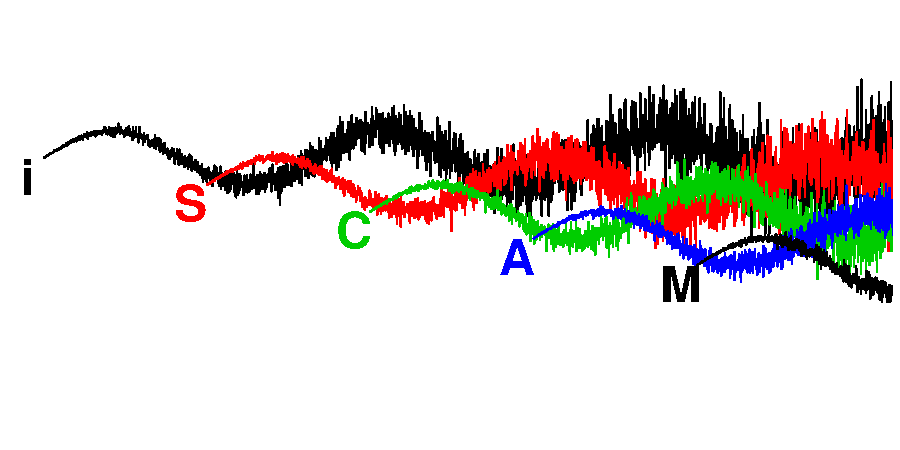
\includegraphics[height=0.53in]{iscamlogo.eps}
%%	}
%%	\pagestyle{fancy}


%-------------------------------------------------------------------------
%Water mark
\usepackage{eso-pic}
\usepackage{graphicx}
\usepackage{color}
\usepackage{type1cm}
\usepackage{float} 

\makeatletter
  \AddToShipoutPicture{%
    \setlength{\@tempdimb}{.6\paperwidth}%
    \setlength{\@tempdimc}{.45\paperheight}%
    \setlength{\unitlength}{1pt}%
    \put(\strip@pt\@tempdimb,\strip@pt\@tempdimc){%
      \makebox(0,0){\rotatebox{45}{\textcolor[gray]{0.85}{\fontsize{2.00cm}{1.75cm}\selectfont{DRAFT  \today\ DRAFT}}}}
    }
} \makeatother


%% -math-
\newcounter{saveEq}
  \def\putEq{\setcounter{saveEq}{\value{equation}}}
  \def\getEq{\setcounter{equation}{\value{saveEq}}}
  \def\tableEq{ % equations in tables
    \putEq \setcounter{equation}{0}
    \renewcommand{\theequation}{T\arabic{table}.\arabic{equation}}
    \vspace{-5mm}
    }
  \def\normalEq{ % renew normal equations
    \getEq
    \renewcommand{\theequation}{\arabic{section}.\arabic{equation}}}

  \def\puthrule{ %thick rule lines for equation tables
    \hrule \hrule \hrule \hrule \hrule}


%%\newcommand{\msy}{$C^*$}
%%\newcommand{\fmsy}{$F^*$}
%%\newcommand{\sbmsy}{$\rm{SB_{MSY}}$}
%%\newcommand{\sbfour}{$\rm{SB_{40}}$}
%%\newcommand{\�}{\'e}
%%\newcommand{\�}{\`e}
%%\newcommand{\�}{\`a}
%%\newcommand{\�}{\^e}
\newcommand{\iscam}{
{$^i$}\textcolor{red}{S}\textcolor{green}{\small{}C}{\textcolor{blue}{\footnotesize{}A}}\textcolor{black}{$_\textnormal{M}$}}%{\raisebox{-0.7ex}{M}}%

\newcommand{\fmsy}{F$_{\textnormal{MSY}}$}
\newcommand{\bmsy}{B$_{\textnormal{MSY}}$}

%% ---------------------------------------------------------------------


\makeatletter
\newenvironment{tablehere}
  {\def\@captype{table}}
  {}

\newenvironment{figurehere}
  {\def\@captype{figure}}
  {}
\makeatother

%% ---------------------------------------------------------------------


\title{
%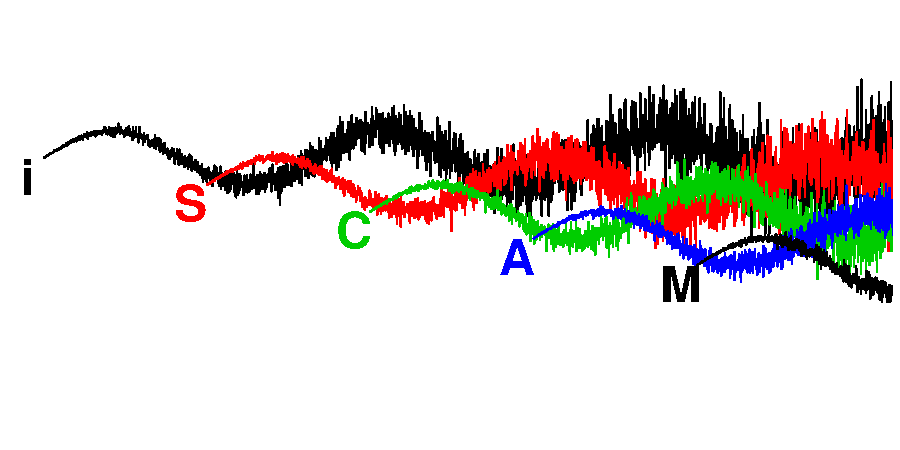
\includegraphics[height=2.53in]{iscamlogo.eps}
Part I\\Moving towards the sustainable fisheries framework for Pacific herring: data, models, and alternative assumptions. \vfill
Part II\\Stock Assessment and Management Advice for the British Columbia Pacific Herring Stocks:\\ 2011 Assessment and 2012 Forecasts
\vfill
}



\author{Steven Martell, Jake Schweigert, Jaclyn Cleary, Vivian Haist}

\date{\vfill \today}







\begin{document}

\pagenumbering{roman}
\setcounter{page}{1}
    \maketitle \thispagestyle{empty}
%    \vfill
%    \noindent\hrulefill\\
%    Draft document for peer review: Started on Wednesday, February 11, 2009\\
%    Draft document completed on Thursday, February 19, 2009\\
%    Final document completed on Wednesday, March 4, 2009.\\
%    CSAS revisions completed on Wednesday, March 11, 2009.
%    \clearpage
\thispagestyle{empty}
\clearpage


\newpage


%\begin{abstract}
%This is the abstract
%  \end{abstract}
%\clearpage


%%
 \selectlanguage{english}

    %\input{ToDoList}
%% -Executive summary material------------------------------------------

\pagenumbering{roman}
\subsection*{Abstract}
\addcontentsline{toc}{subsection}{Abstract}

June 15, 2011.  Structure of this paper has changed a bit. This document will now consist of an assessment and forecast of the five major stocks and the two minor stocks.  There will be at least 5 appendixes that 1) describe the input data and the control files used for the assessment model, 2) a detailed description of \iscam, 3) a description of the methods used to develop the prior distribution, 4) simulation testing of the \iscam model, 5) moving toward the sustainable fisheries framework (see Cleary and Cox paper) and include discussion of the issues of developing an MSY-based framework for a multigear fishery with changing selectivities and natural mortality rates, and finally 6) a list of research recommendations.

Summary:  Three major themes of the paper: 1) a comparing HCAM and iSCAM (where iSCAM is set up with nearly the same assumptions as 2010 HCAM assessment), 2) an iSCAM assessment with several scenarios addressing (a) q with various priors, (b) time-varying versus constant M, (c) alternative selectivity models, and (d) the interactions of all three of these confounded variables, and 3) an iSCAM assessment with the test fishery and seine roe fishery data separated into specific fleets.  The side by side comparison will examine similarities/differences between trends in biomass, fishing mortality rates, and residual fits to the spawn survey data an age-composition data.  These two models have some fundamental differences in the statistical assumptions about the catch-at-age data, so results are likely to be slightly different.  Results for all three themes will focus on reconstructing table 5 from last years assessment, with the addition of LRP and USRP to be compared with the cuttoffs and catch advice for low med and high recruitment.






%%%!TEX root = /Users/stevenmartell/Documents/CURRENT PROJECTS/iSCAM-trunk/fba/BC-herring-2011/WRITEUP/BCHerring2011.tex


%\subsection*{Abstract}
%\addcontentsline{toc}{subsection}{Abstract}
%
%June 15, 2011.  Structure of this paper has changed a bit. This document will now consist of an assessment and forecast of the five major stocks and the two minor stocks.  There will be at least 5 appendixes that 1) describe the input data and the control files used for the assessment model, 2) a detailed description of \iscam, 3) a description of the methods used to develop the prior distribution, 4) simulation testing of the \iscam model, 5) moving toward the sustainable fisheries framework (see Cleary and Cox paper) and include discussion of the issues of developing an MSY-based framework for a multigear fishery with changing selectivities and natural mortality rates, and finally 6) a list of research recommendations.
%
%Summary:  Three major themes of the paper: 1) a comparing HCAM and iSCAM (where iSCAM is set up with nearly the same assumptions as 2010 HCAM assessment), 2) an iSCAM assessment with several scenarios addressing (a) q with various priors, (b) time-varying versus constant M, (c) alternative selectivity models, and (d) the interactions of all three of these confounded variables, and 3) an iSCAM assessment with the test fishery and seine roe fishery data separated into specific fleets.  The side by side comparison will examine similarities/differences between trends in biomass, fishing mortality rates, and residual fits to the spawn survey data an age-composition data.  These two models have some fundamental differences in the statistical assumptions about the catch-at-age data, so results are likely to be slightly different.  Results for all three themes will focus on reconstructing table 5 from last years assessment, with the addition of LRP and USRP to be compared with the cuttoffs and catch advice for low med and high recruitment.
%


\section*{Abstract}\addcontentsline{toc}{section}{Abstract}

Estimates of herring abundance in British Columbia (B.C.) waters  has been based on catch-age data and spawn survey abundance information.  These data are typically interpolated using a statistical catch-age framework; however, virtual methods (e.g., VPA) have been used in the past.  This document is broken into two parts: Part I deals with moving the herring assessments towards Canada's sustainable fisheries framework and introduces a new integrated statistical catch-age model for jointly estimating the abundance of Pacific herring and associated reference points to be used in the sustainable fisheries framework.  Part II of this document actually implements this new assessment framework using the data for the five major and two minor regions.  Finally, we present catch advice based on decision tables that utilize poor, average, and good age-3 recruitment forecasts.

In Part I of this document we provide a very brief description of the new assessment framework (a full technical description of the model is provided in the Appendix of this document).  We then conduct some simulation testing with perfect information to  demonstrate that the model is capable of estimating all the parameters. We further explore precision and bias in parameter estimates based on simulation data with both observation and process errors.  We then parameterize the new assessment model such that most of the assumptions of the previous assessment model (Herring Catch Age Model, or HCAM) are mostly met and compare parameter estimates and estimates of spawning stock biomass (using data from 1951:2010).  Using data from the Strait of Georgia only, we then compare alternative assumptions about the spawn survey scaling coefficient ($q$), natural mortality and selectivity, and examine how these alternative assumptions influence estimates of key parameters (unfished spawning biomass, steepness, average natural mortality).  Relaxing assumptions about $q$ and natural mortliaty rates had the largest impacts on estimated parameters.  Lastly, we compared estimates of spawning stock biomass from HCAM with the new model for all five major areas to understand the subtle differences between the assumptions in the two models \footnote{At the time of writing this document and submitting it for peer review, an error was notices in the formulation of the weight-based selectivity function for the gill net fishery.  This error has been corrected for all of the results presented in Part II, but has still to be corrected for the model comparisons in Part I of this document.  Time permitting, these comparisons will be conducted prior to the assessment meeting, and if not at least presented at the September 7, 2011 meeting.}.

In Part II of this document we present updated data from the herring fisheries and surveys in 2011, a brief description of the analytical methods used to construct the decision tables, and present the results of the application of the new assessment model to the 2011 data. New this year is a Bayesian prior for the dive survey spawn index ($q$) and the development of this prior is detailed in the appendix.  The expected value of $q$ was estimated to be 0.587 with a standard deviation of 0.155. To summarize the overall fit to the model, maximum likelihood estimates derived quantities and residuals between observed and predicted variables are used.  Retrospective analysis (i.e., the sequential removal of the most recent data) is used as a diagnostic for model misspecification.   Catch advice (decision tables) are based on the median values of random samples from the joint posterior distribution and not the maximum likelihood estimates.  Visual inspection of the trace plots from the posterior samples and pair plots were used to judge if the samples were taken from a stationary distribution. Historically catch advice was based on cuttoff values that were derived from 1996 estimates of the unfished biomass (\bo, cuttoff values are set at 0.25\bo).  This assessment provides updated estimates of \bo and presents catch advice based on new cuttoff values.  An alternative decision table, where catch advices is based on old cuttoffs, is also presented.  

Median estimates of the 2011 spawning stock biomass is as follows: Haida Gwaii (HG) --16,579 t, Prince Rupert District (PRD) -- 27,046 t, Central Coast (CC) -- 14,666 t, Strait of Georgia (SOG) 125,261 t, West Coast Vancouver Island (WCVI) 14,679 t.  Implementation of the current harvest control rule (HCR) advises no fishing in HG under poor recruitment and no fishing in CC under poor and average recruitment.  Based on the 20\% harvest rate and application of the harvest control rule the estimated maximum available harvest ranges from 4,296 t in HG to 27,690t in SOG (assuming good recruitment).  Catch advice for the minor areas is based on a 10\% fixed exploitation rate with no cuttoffs and ranges from 91 t in Area 27 (assuming poor recruitment) to 614 t in Area 2W (assuming good recruitment).

%\section*{Executive summary}\addcontentsline{toc}{section}{Executive summary}


\newpage
\tableofcontents
\addcontentsline{toc}{subsection}{Contents}
\newpage

\listoffigures
\addcontentsline{toc}{subsection}{List of Figures}
\newpage
%% -Main body of the document-------------------------------------------
\pagenumbering{arabic}


%!TEX root = /Users/stevenmartell/Documents/CURRENT PROJECTS/iSCAM-trunk/fba/BC-herring-2011/WRITEUP/BCHerring2011.tex

%% PART I
\part{Moving towards a sustainable fisheries framework for Pacific herring: data, models and alternative assumptions}

\addtocounter{chapter}{1}

%% SECTION Introduction
\section{Introduction}
	
There are four major objectives of this paper: (1) to describe in detail an alternative integrated statistical catch-age model (iSCAM), (2) examine parameter estimation performance using iSCAM, (3) perform a side-by-side comparison of the previous HCAM and iSCAM on the five major herring stocks, and (4) explore alternative assumptions about selectivity, catchability, and natural mortality using iSCAM.  The most recent assessment of BC herring stocks was conducted in 2010 using the Herring Catch Age Model (HCAMv2) which is documented in \cite{Clear2010}.  Furthermore, a review sponsored by the Herring Research and Conservation Society (HRCS) was conducted June 17-18, 2010 in Nanaimo, BC where an expert panel addressed specific questions about the current implementation of the HCAMv2 model and suggested recommendations for each of the questions.  This paper also attempts to address some of the points brought up in the review.

BC herring are currently managed as five major stocks and 2 minor stocks (Figure \ref{Fig1}).  Annual catch advice for each of these areas is based on current estimates of stock status, and a 20\% exploitation rate if the stock is above the cutoff level for the five major stocks and a 10\% exploitation rate for the two minor stocks.  Cutoff levels for the five major stocks are based on 0.25$B_o$, and estimates of unfished biomass were established first in 1985 \citep{haist1986stock}.  These cutoffs are currently are thought to be more conservative 	than the current default Limit Reference Point of 0.4\bmsy\ \citep{dfo2006}. However, estimates of $B_o$ and MSY based reference points have not been examined for Pacific herring for some time.  In this paper we also describe the methods for updating estimates of $B_o$ and MSY based reference points using the iSCAM model framework.  We also compare estimates of MSY based reference points for the Strait of Georgia herring under the previously mentioned alternative assumptions (see point (4) in the previous paragraph).

We do not provide a detailed description of HCAMv2 in this paper and we refer the reader to \cite{schweigert2009stock} and \cite{Clear2010} for a more detailed description.  We first begin with a description of the input data required and assumptions about the data, followed by a detailed description of the analytical methods and assumptions in iSCAM. We then present the analytical methods and assumptions for exploring alternative hypotheses about selectivity, catchability and natural mortality, followed by a description of the elements that make up the joint posterior distribution (i.e., likelihoods, priors, and penalties).  Parameter estimating and quantifying uncertainty is carried out using AD Model Builder \citep{ADMB2009}.  We then explore estimation performance in iSCAM using simulation experiments where the model is used to generate simulated observations with known parameter values, then estimate parameter, and repeat this exercise a number of times to evaluate bias and precision in parameter estimates.  Finally, we present forecast of pre-fishery biomass and available harvest options using the cutoffs \cite[e.g., reproduce Table 5 in ][]{Clear2010} as well as available harvest options based on the Sustainable Fisheries Framework \citep[i.e.,][]{dfo2006} for comparison.

\begin{figure}[!tbp]
	% Requires \usepackage{graphicx}
	%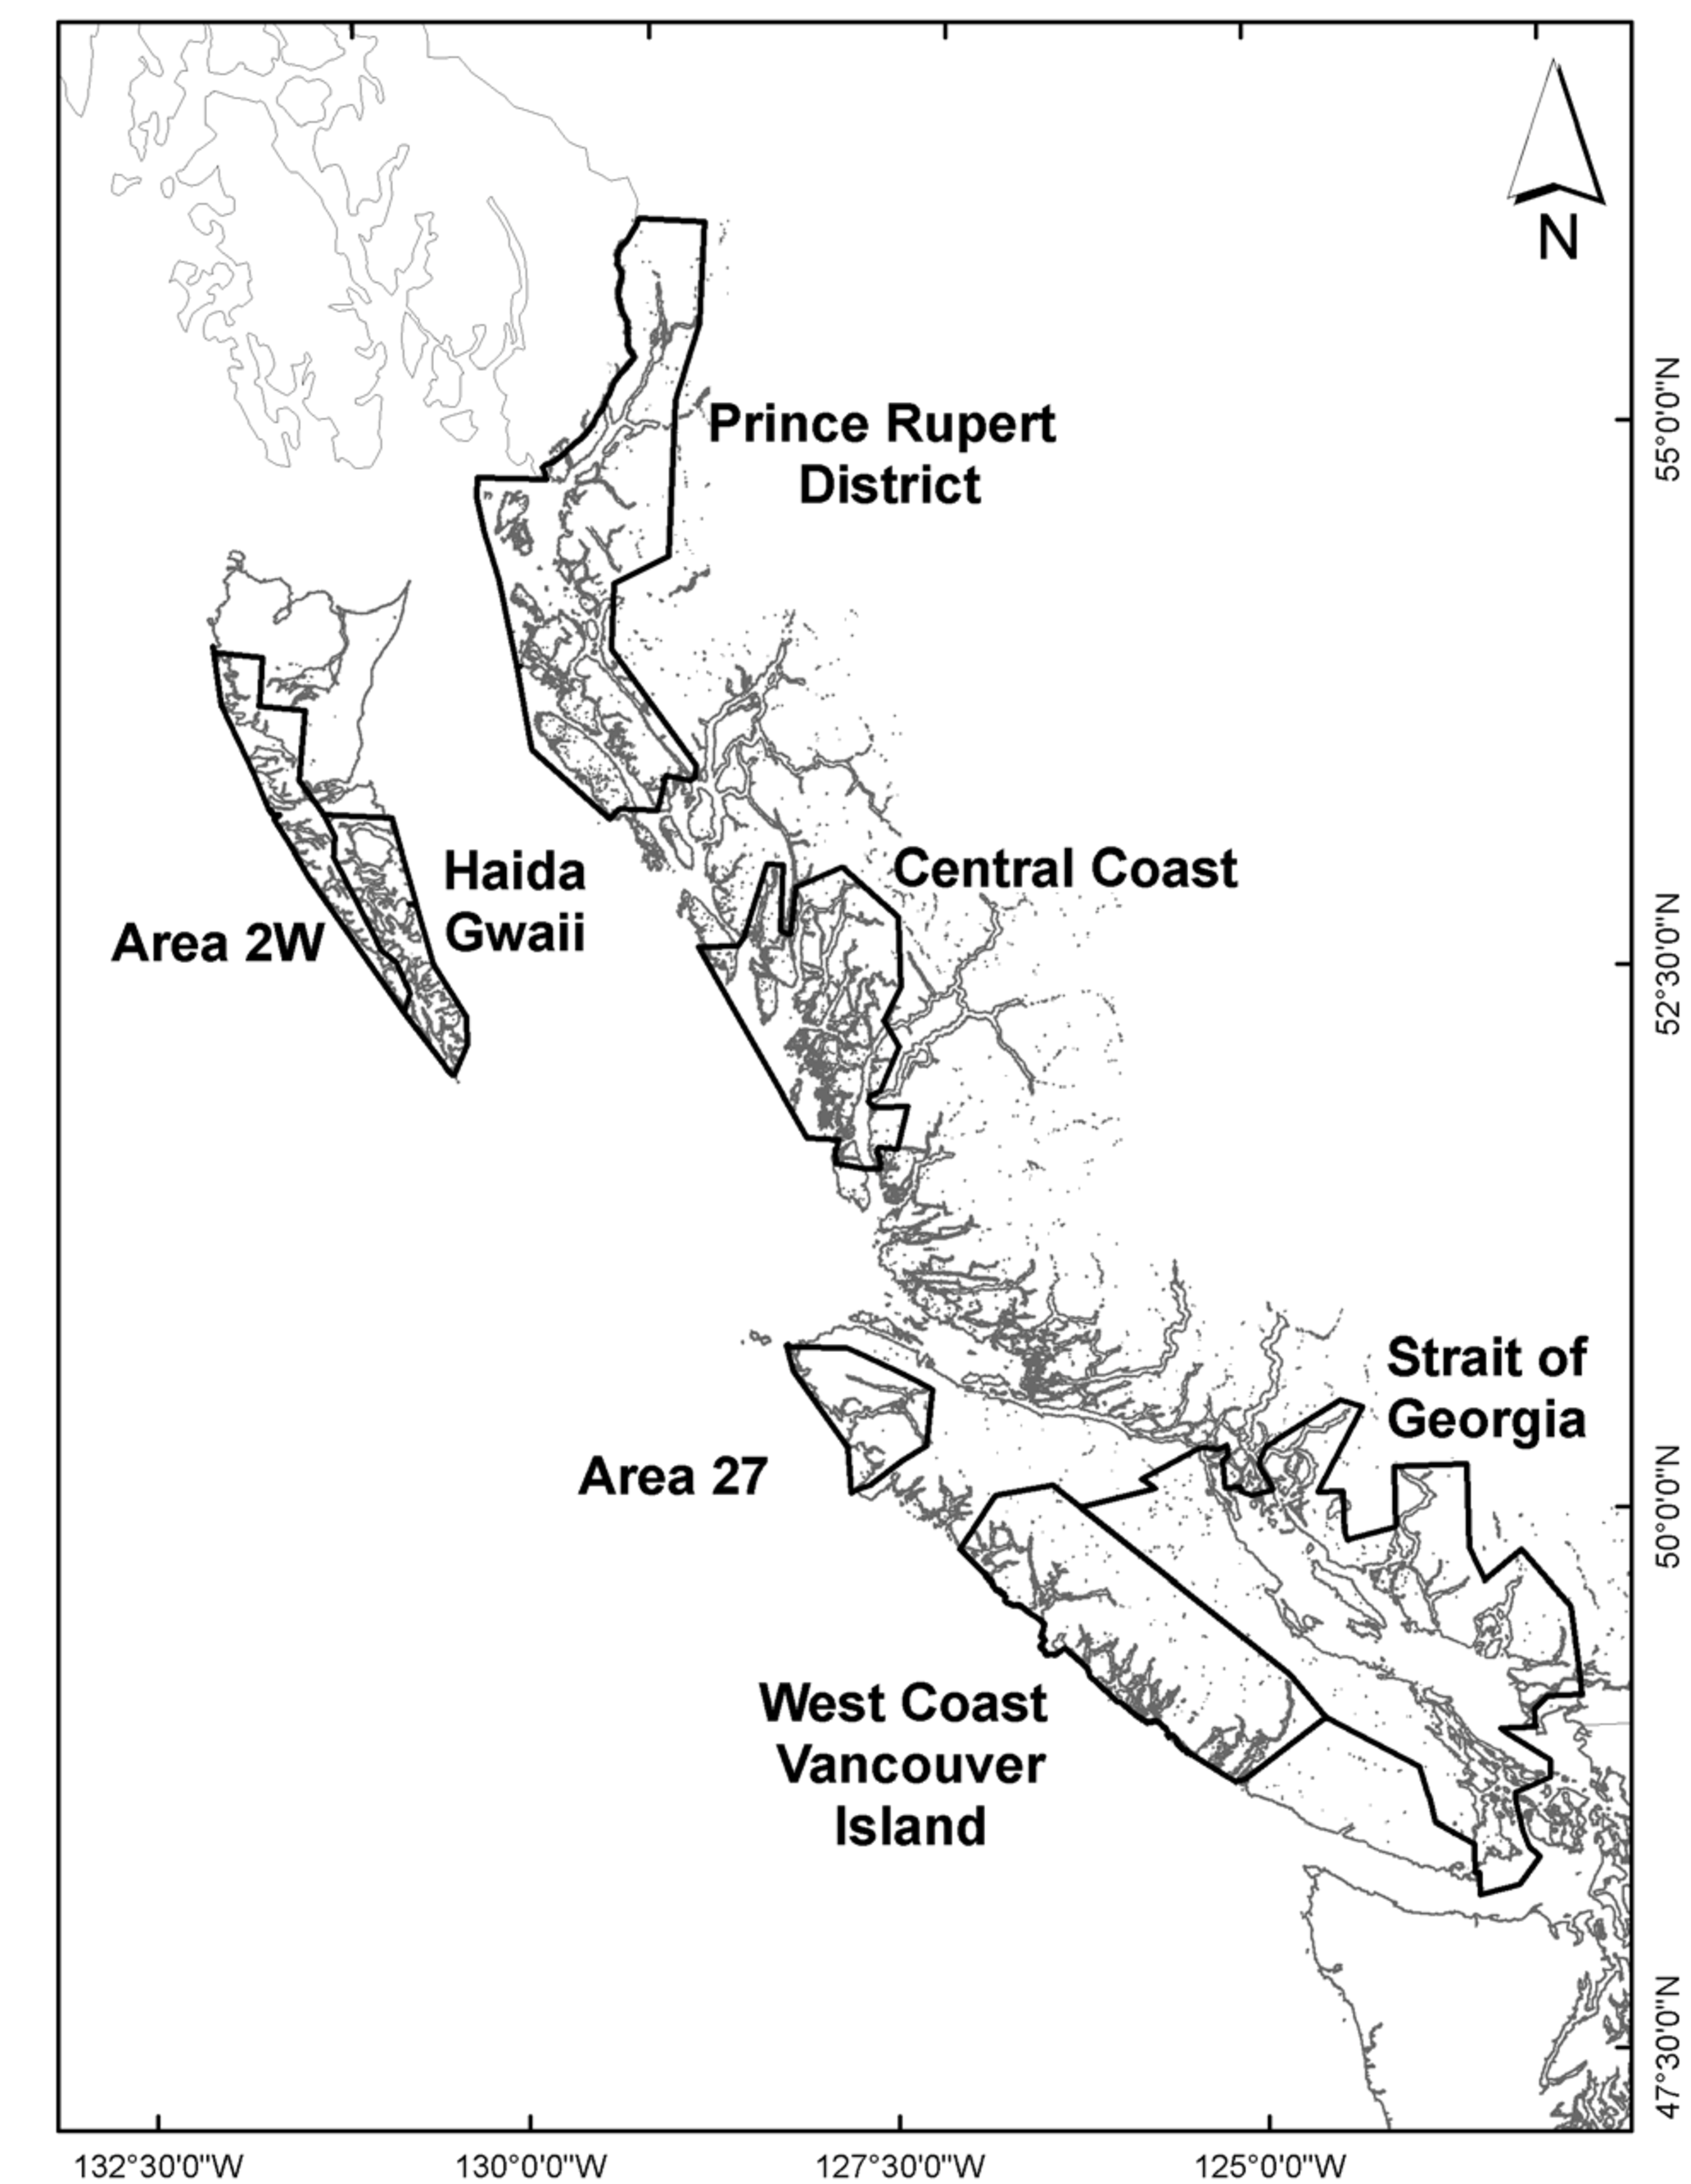
\includegraphics[width=\textwidth]{Figs/HerringAreaMap.pdf}
	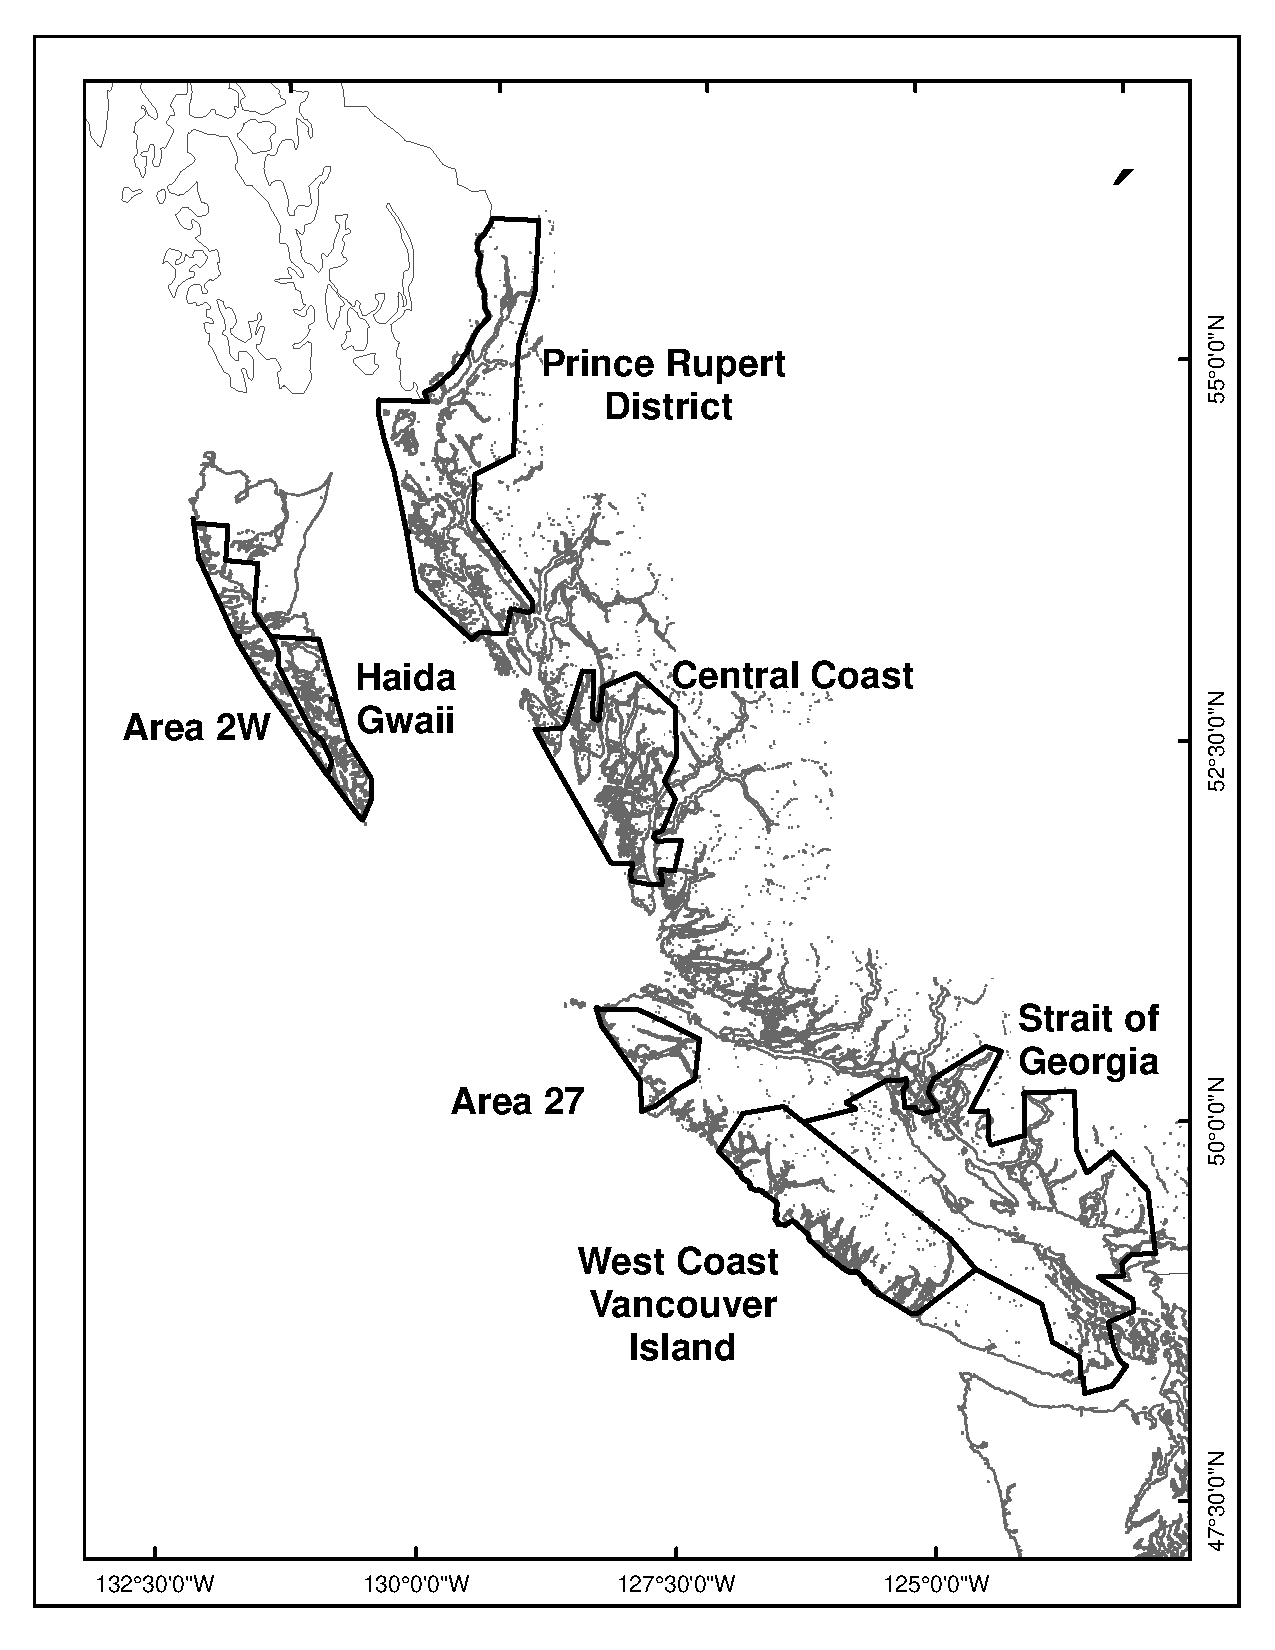
\includegraphics[width=\textwidth]{PBSfigs/Assessment_Regions_2W_27_2010_HG.pdf}
	\caption{B.C. herring major stock areas: Haida Gwaii (HG or QCI 2E), Prince Rupert District (PRD), Central
Coast (CC), Strait of Georgia (SOG), West Coast Vancouver Island (WCVI), and minor stock areas: Area 2W and
Area 27.}\label{Fig1}
\end{figure}
	
%%A reference for splines in selectivities can be found at \cite{aarts2009comprehensive}


%% SECTION Methods
%!TEX root = /Users/stevenmartell/Documents/CURRENT PROJECTS/iSCAM-trunk/fba/BC-herring-2011/WRITEUP/BCHerring2011.tex
\section{Methods}
	\subsection{Input data \& assumptions}
	\subsubsection{Catch data}
	For each of the statistical areas, the required input data for \iscam\ consists of a catch time series for each of the fishing fleets.  For the BC herring fishery, the annual total removals has been partitioned into three distinct fishing fleets (or fishing periods, see Figure \ref{FigCatch}).  The first fleet is a winter seine fishery that has been in operation since the start of the assessment in 1951, the second is a seine-roe fishery that commenced in 1972 in the Strait of Georgia, and the third fleet is a gillnet fishery that targets females on the spawning grounds. The model is fit to the catch time series information and assumes measurement errors are lognormal, independent and identically distributed.  The assumed standard deviation in the catch observations must be specified in the control file and it is assumed that measurement errors in the catch is the same for all fishing periods.  The units of the catch are given in 1000s of metric tons.
	
	In addition to the commercial catch, removals from fisheries independent surveys must also be specified in \iscam. Two additional fleets are specified to represent the spawn survey, where the spawn survey is broken into two distinct time periods pre-1988 and post-1988, the year when the survey switched from surface surveys to dive surveys.  This partitioning of the data is done for two reasons: (1) to allow for different catchability coefficients to be specified for the early and late periods, and to allow for more weight to be placed on the contemporary data due to improved precision in the estimates of egg layers. 

%TODO decide if the test fishery data is going to be looked at here or in the appendix
	In the case where the test fishery data has been separated from the seine roe fishery, an additional fleet is specified in the data file and fishing mortality rates for the test fishery are also estimated in years when the catch is greater than 0.
	
\begin{figure}[!tbp]
	% Requires \usepackage{graphicx}
	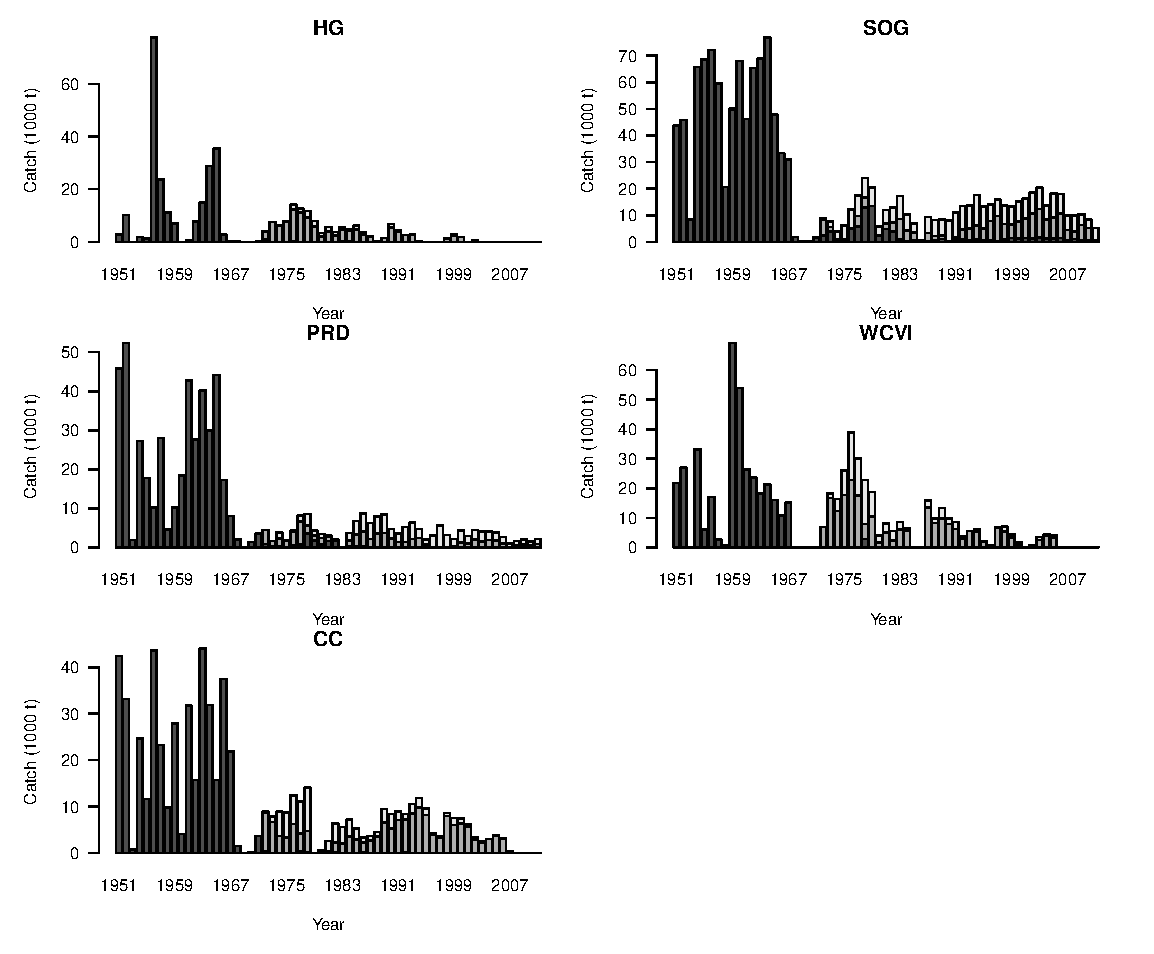
\includegraphics[width=\textwidth]{../Figs/iscam_fig_CatchMajorAreas.pdf}\\
	\caption{Historical catch of herring in the five major stock areas between 1951 and 2011 for the winter purse seine fishery (dark bars), seine-roe fishery (grey bars), and gillnet fishery (light grey bars). Units of catch are in thousands of metric tons.}\label{FigCatch}
\end{figure}
	
	\subsubsection{Relative abundance data}
Herring spawn surveys have been conducted throughout the B.C. coast beginning in the 1930s. Prior to 1988, spawn surveys were conducted from the surface either by walking the beach at low tide or using a drag from a skiff to estimate the shoreline length and width of spawn. Egg layers were sampled visually and are used to calculate egg densities following the methods of \cite{schweigert2001stock}. Beginning in 1988, herring spawn surveys using SCUBA methods were introduced and were implemented coastwide within a couple of years initially being conducted by DFO staff and eventually through contract divers hired through the test fishing program. Prior to the 2006 Larocque ruling, the test fishing program was funded through an allocation of fish by industry. In years since the 2006 Larocque ruling, the availability of resources to conduct dive surveys in all areas has been reduced. For 2011, dive surveys were conducted in all major and minor assessment regions, with the exception of Area 2W where snorkelling and surface survey methods were also used. As in earlier years, a few minor spawning beds outside the main assessment areas were surveyed by SCUBA or surface methods where resources permitted.


The locations of the spawning beds for the five major and two minor stock areas are shown in Figure \ref{figSpawnMaps}.  Egg density estimates are used to calculate a fishery-independent index of herring spawning biomass, referred to as the spawn survey index hereafter \citep{schweigert2001stock}.

\begin{figure}[!tbp]
	% Requires \usepackage{graphicx}
	\centering
	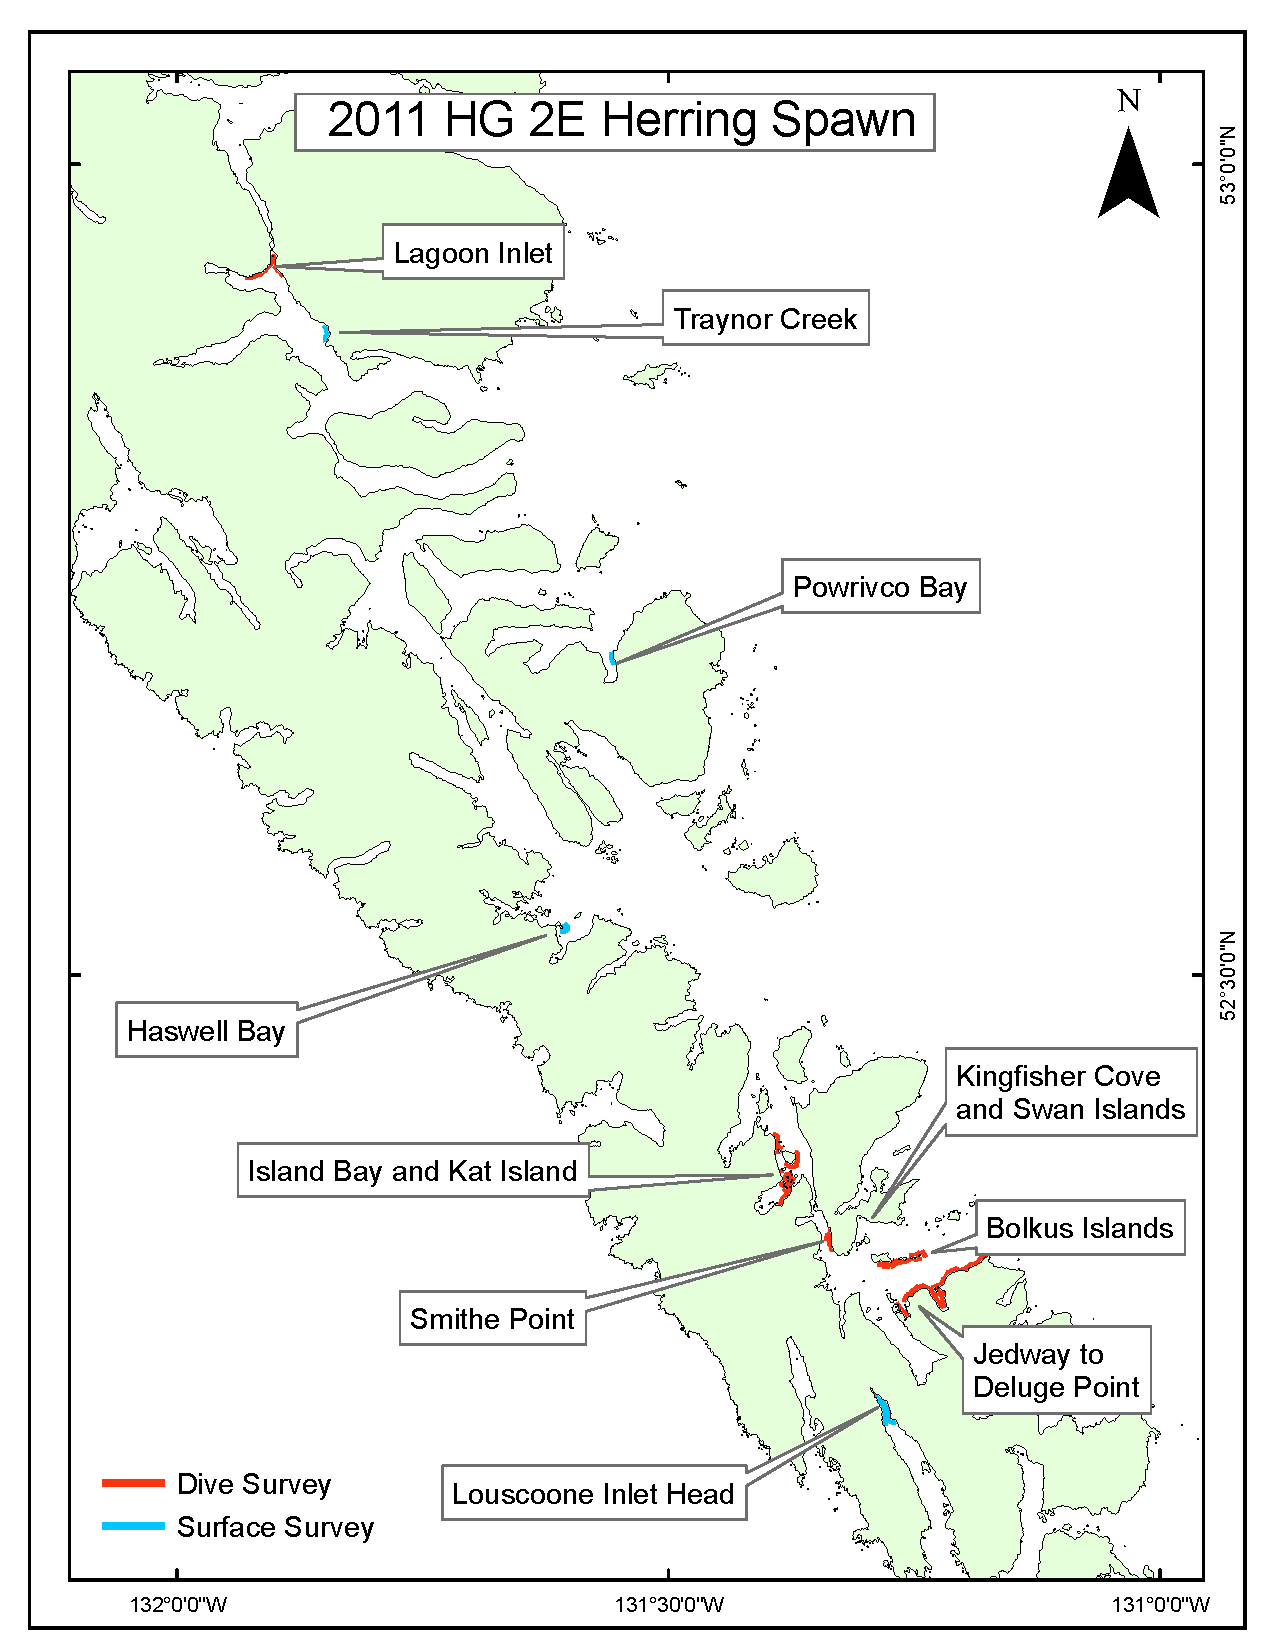
\includegraphics[scale=0.35]{../Figs/PBSfigs/2011_spawn_HG_2E_July13.pdf}
	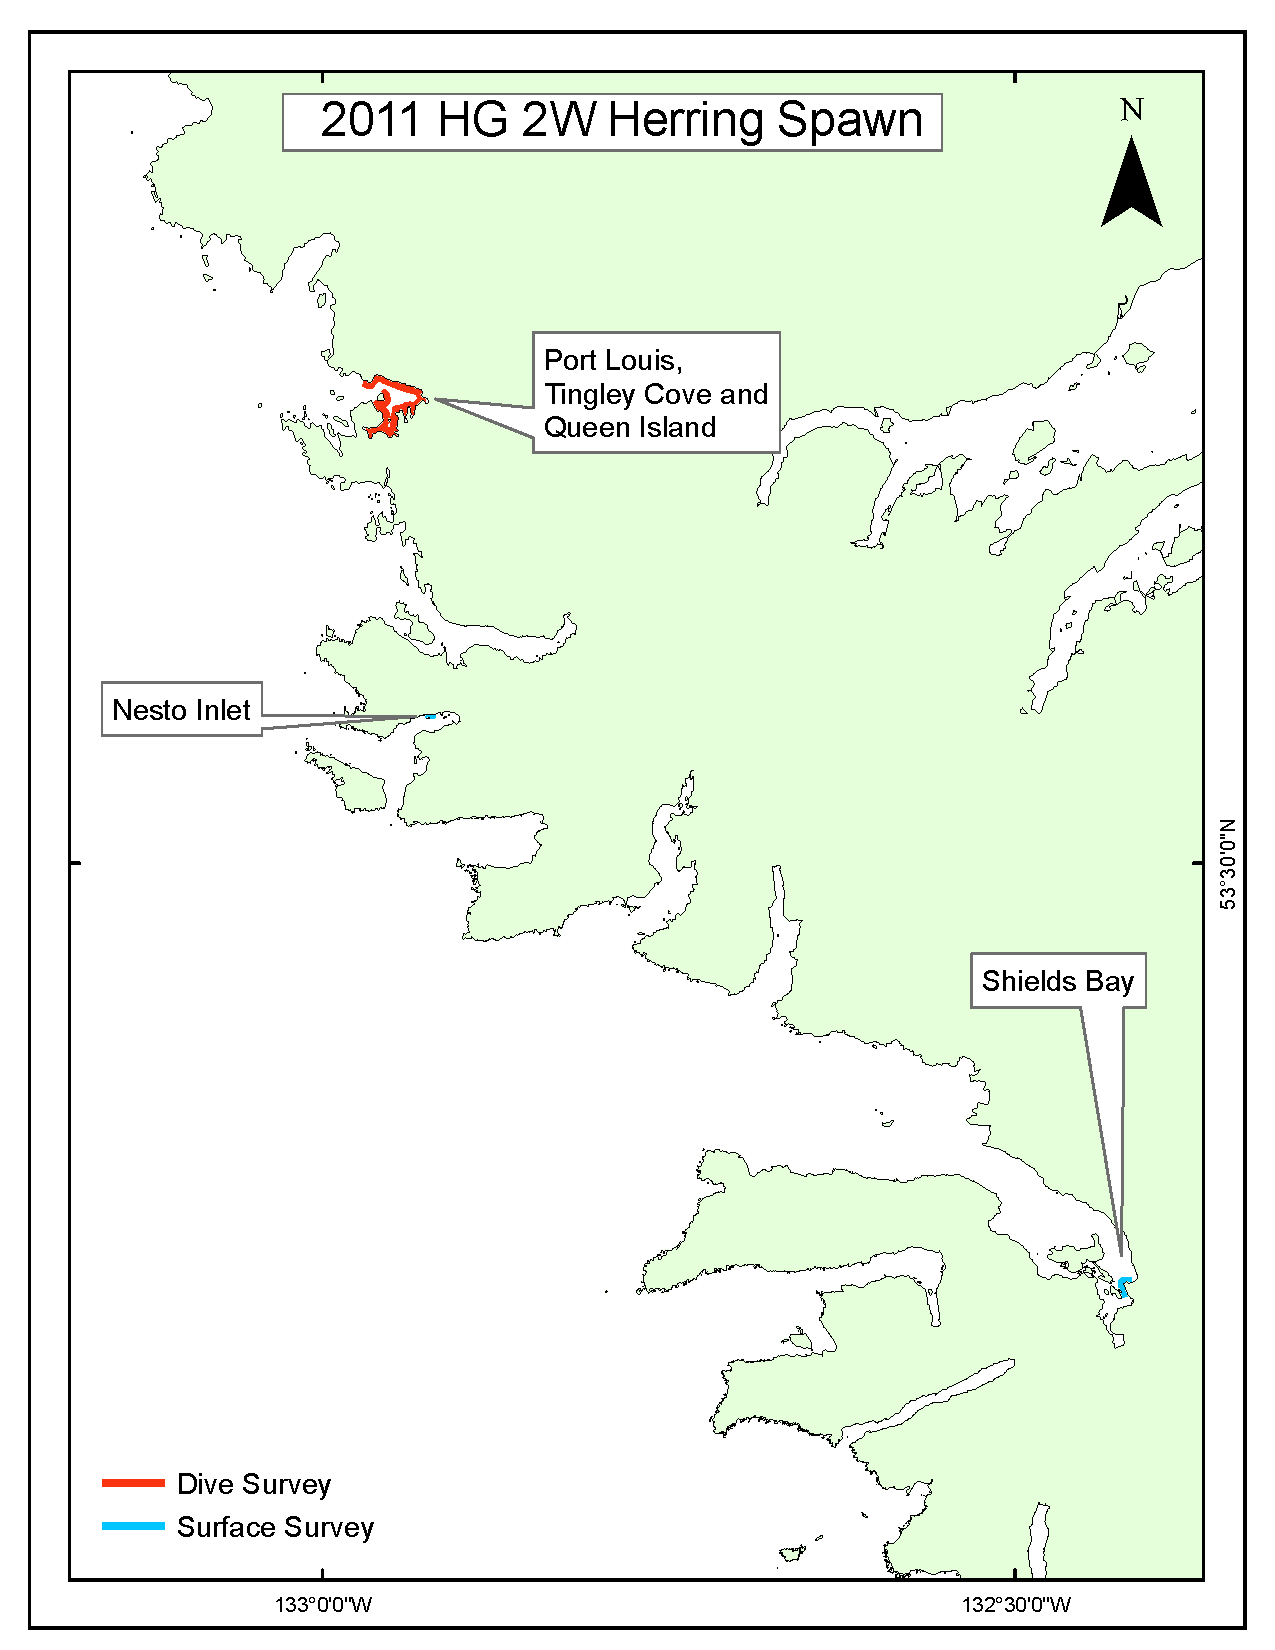
\includegraphics[scale=0.35]{../Figs/PBSfigs/2011_spawn_HG_2W_July13.pdf}\\
	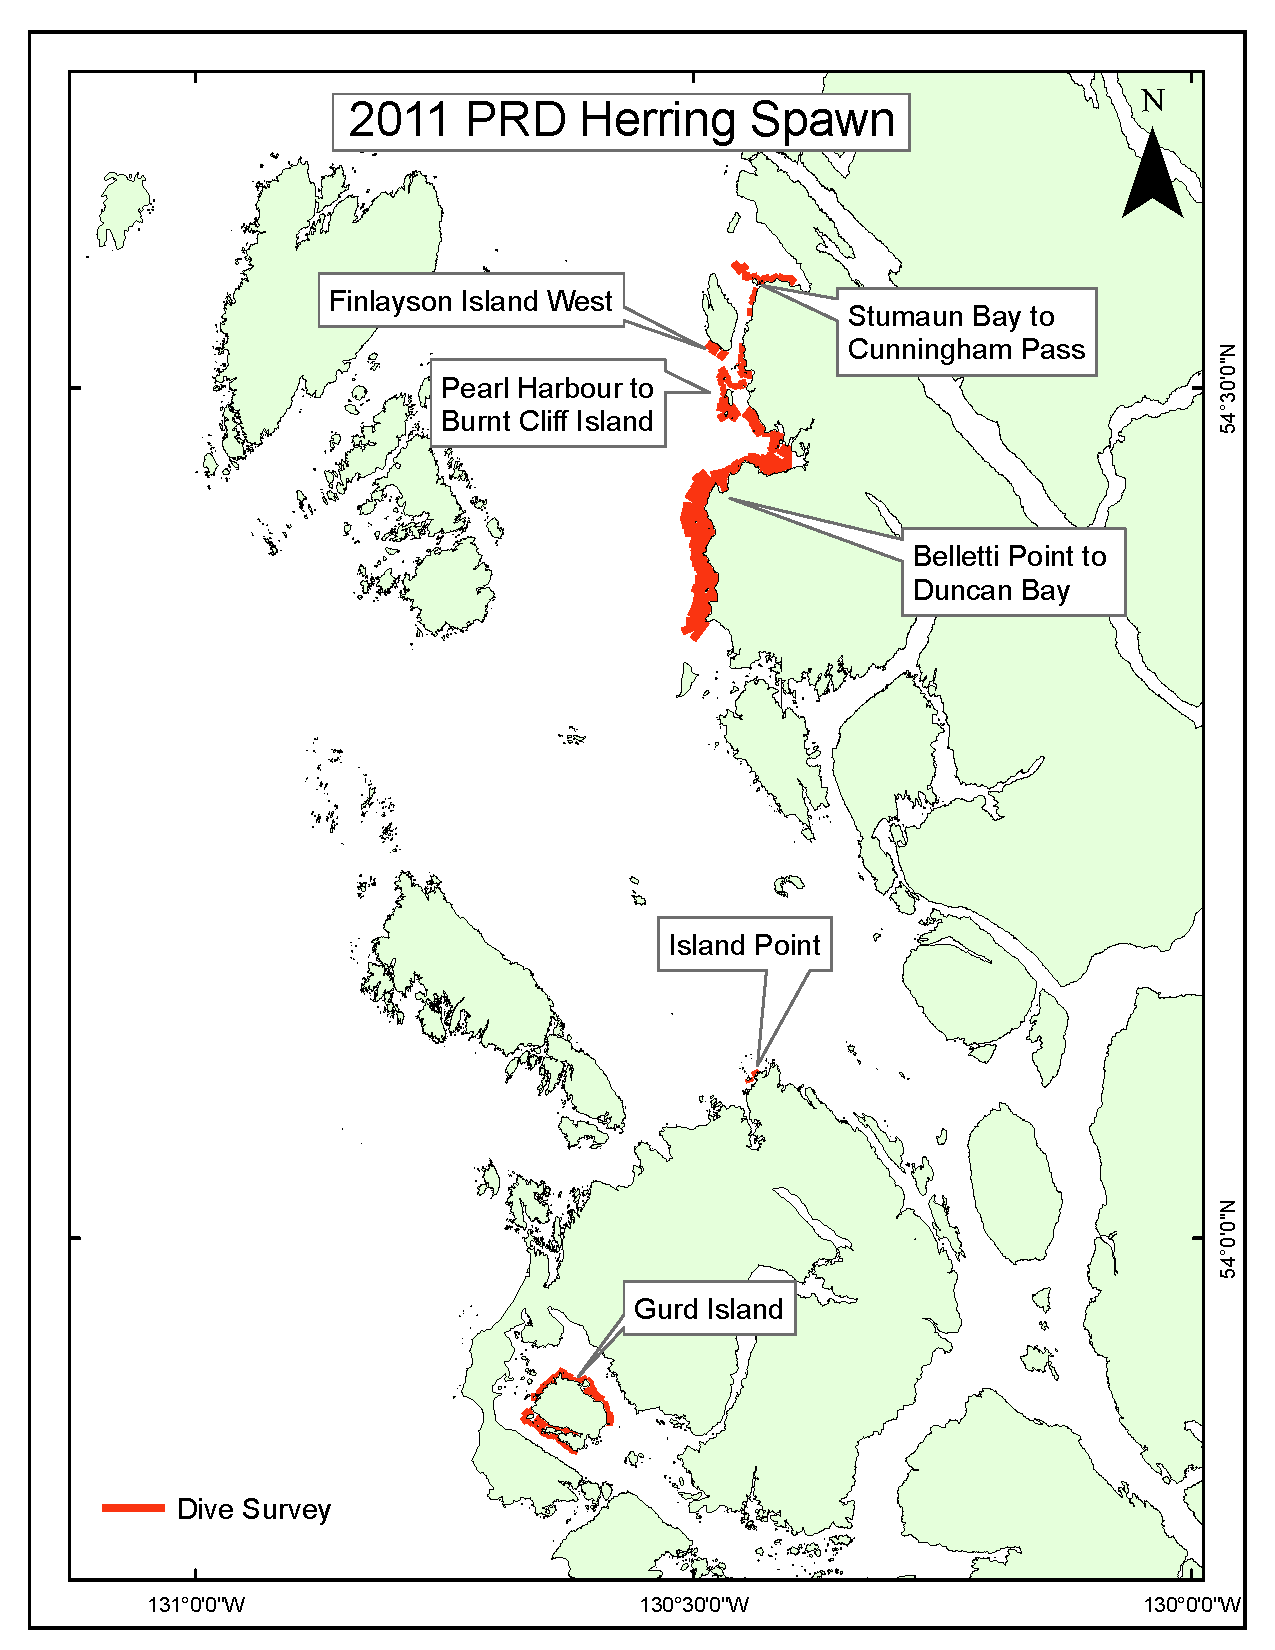
\includegraphics[scale=0.35]{../Figs/PBSfigs/2011_spawn_PRD_July13.pdf}
	\caption{Preliminary Spawning activity for Haida Gwaii (top panels) and Prince Rupert District (bottom) in 2011.}
\end{figure}
\begin{figure}[!tbp]
	% Requires \usepackage{graphicx}
	\ContinuedFloat
	\centering
	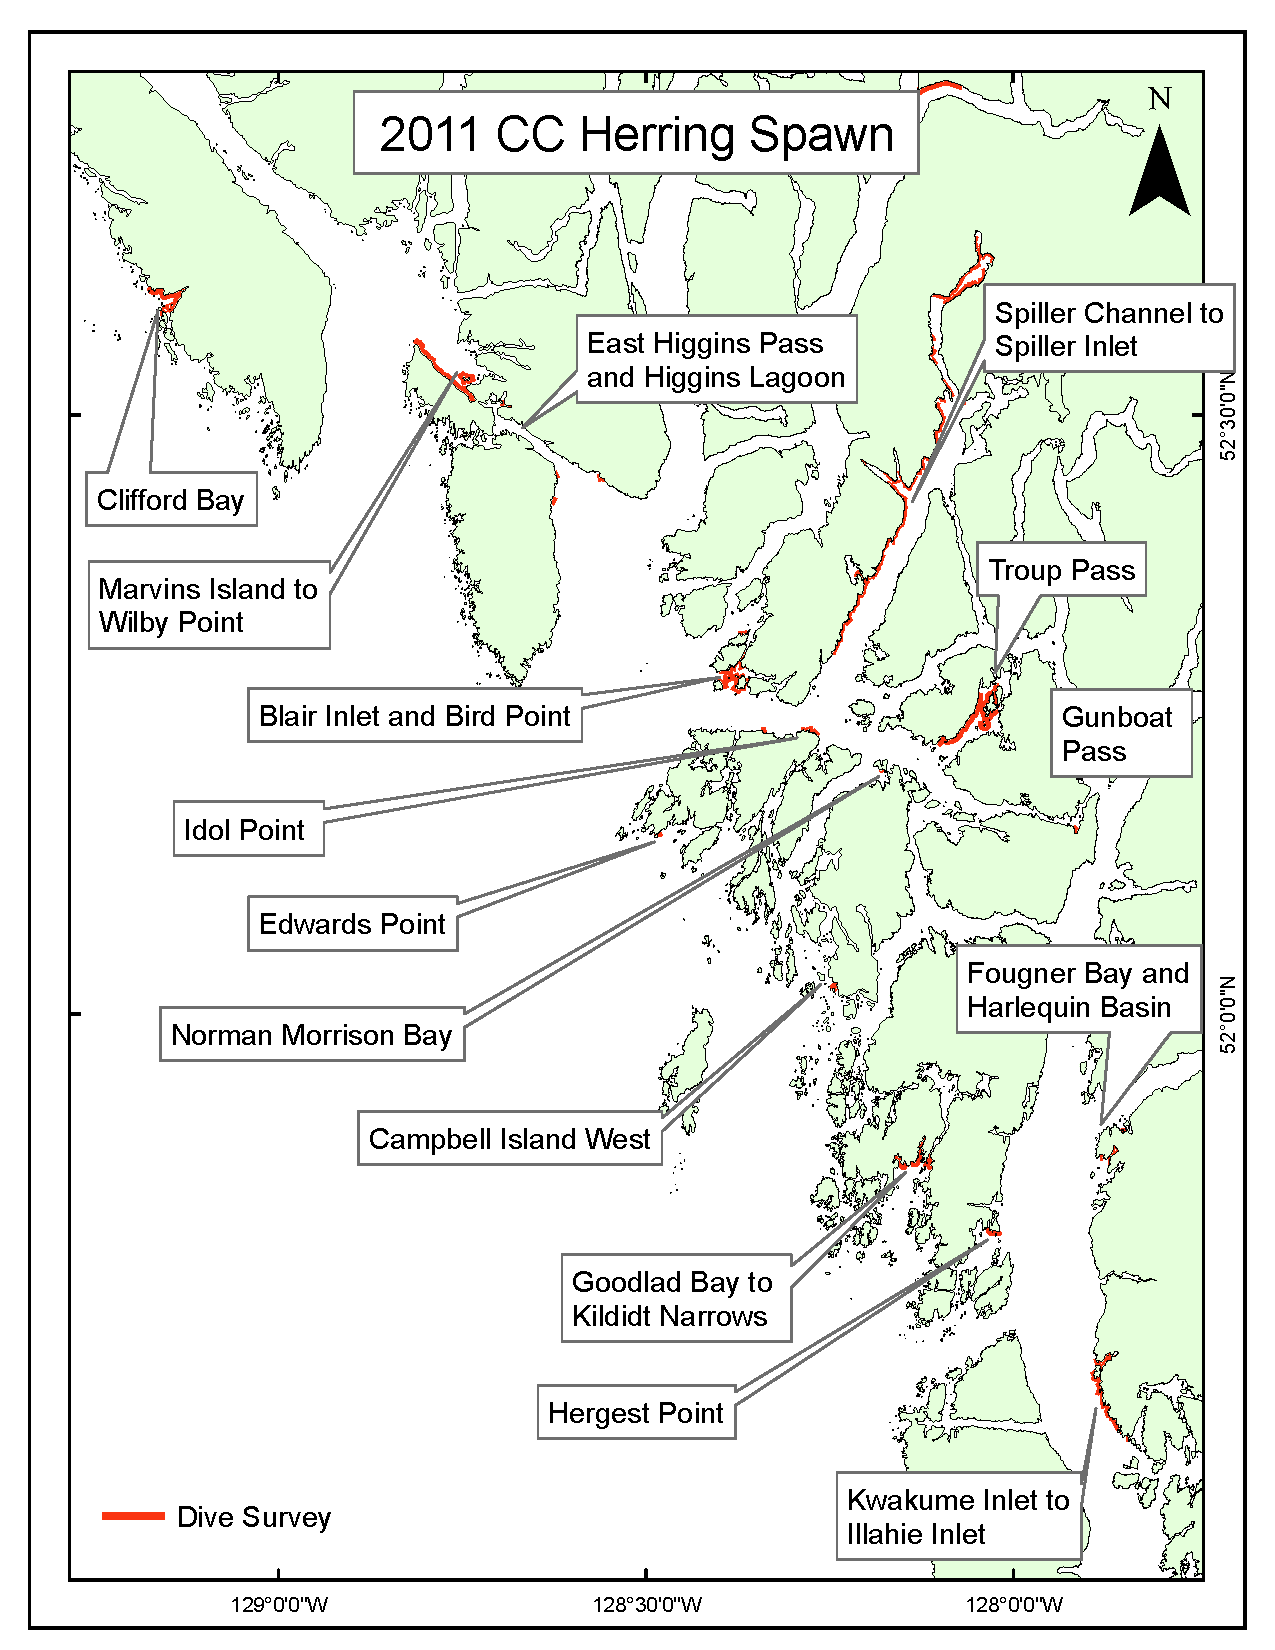
\includegraphics[scale=0.35]{../Figs/PBSfigs/2011_spawn_CCJuly13.pdf}
	%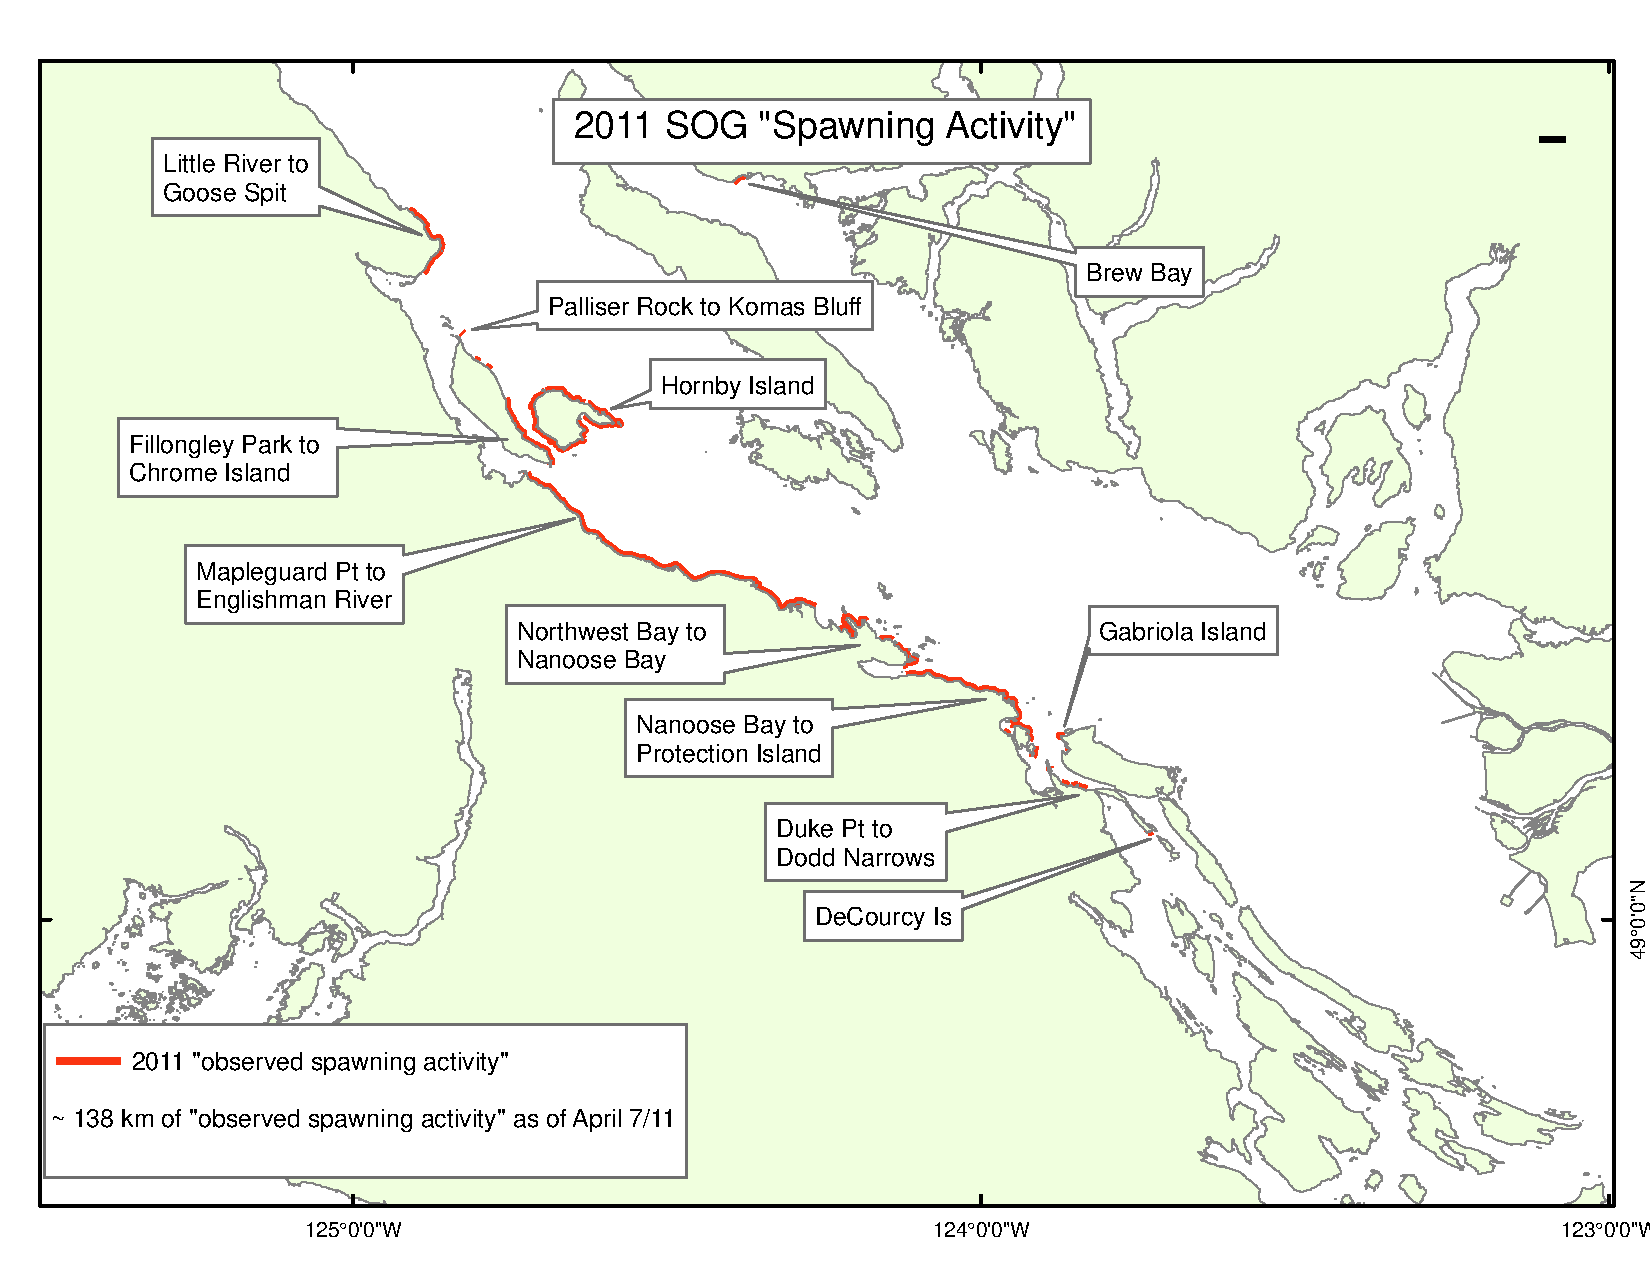
\includegraphics[scale=0.5]{../Figs/PBSfigs/2011-SOG-Prelim-WG.pdf}
	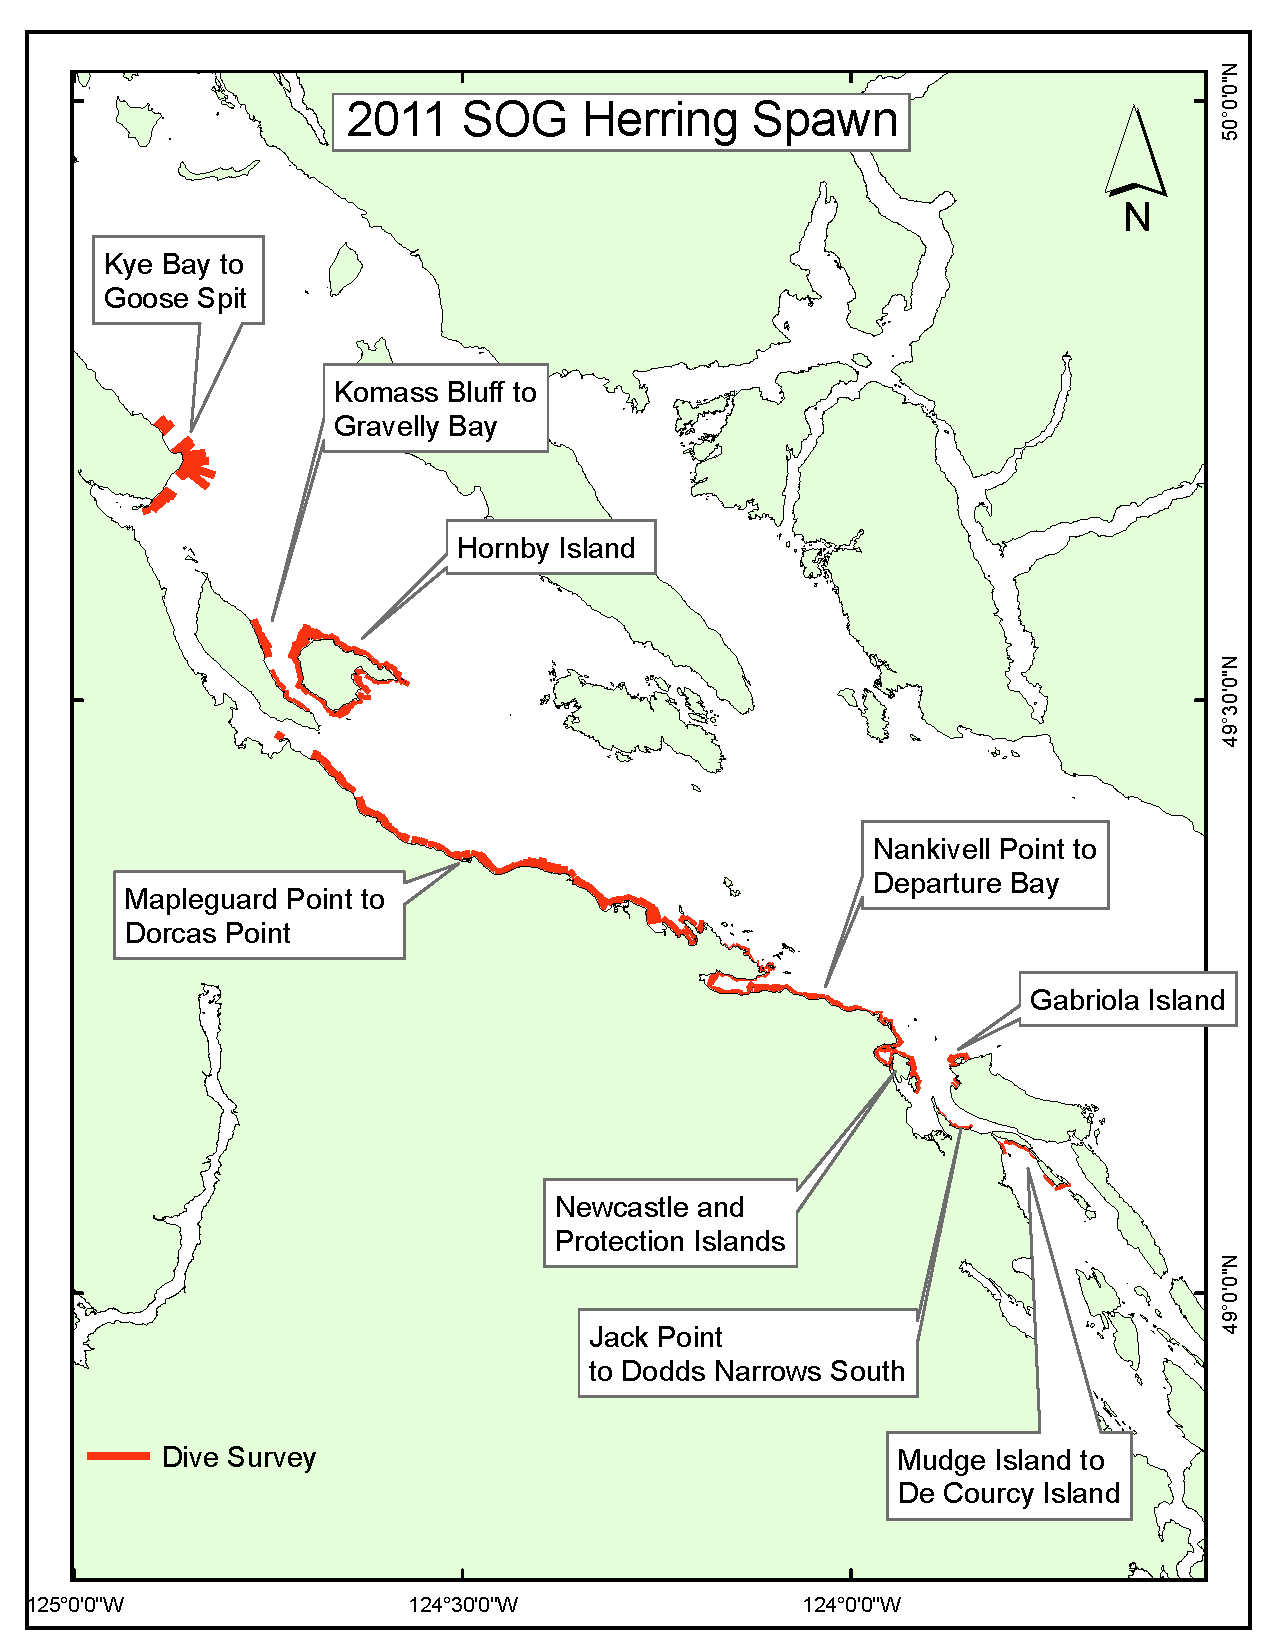
\includegraphics[scale=0.35]{../Figs/PBSfigs/2011_spawn_SOG_July13.pdf}\\
	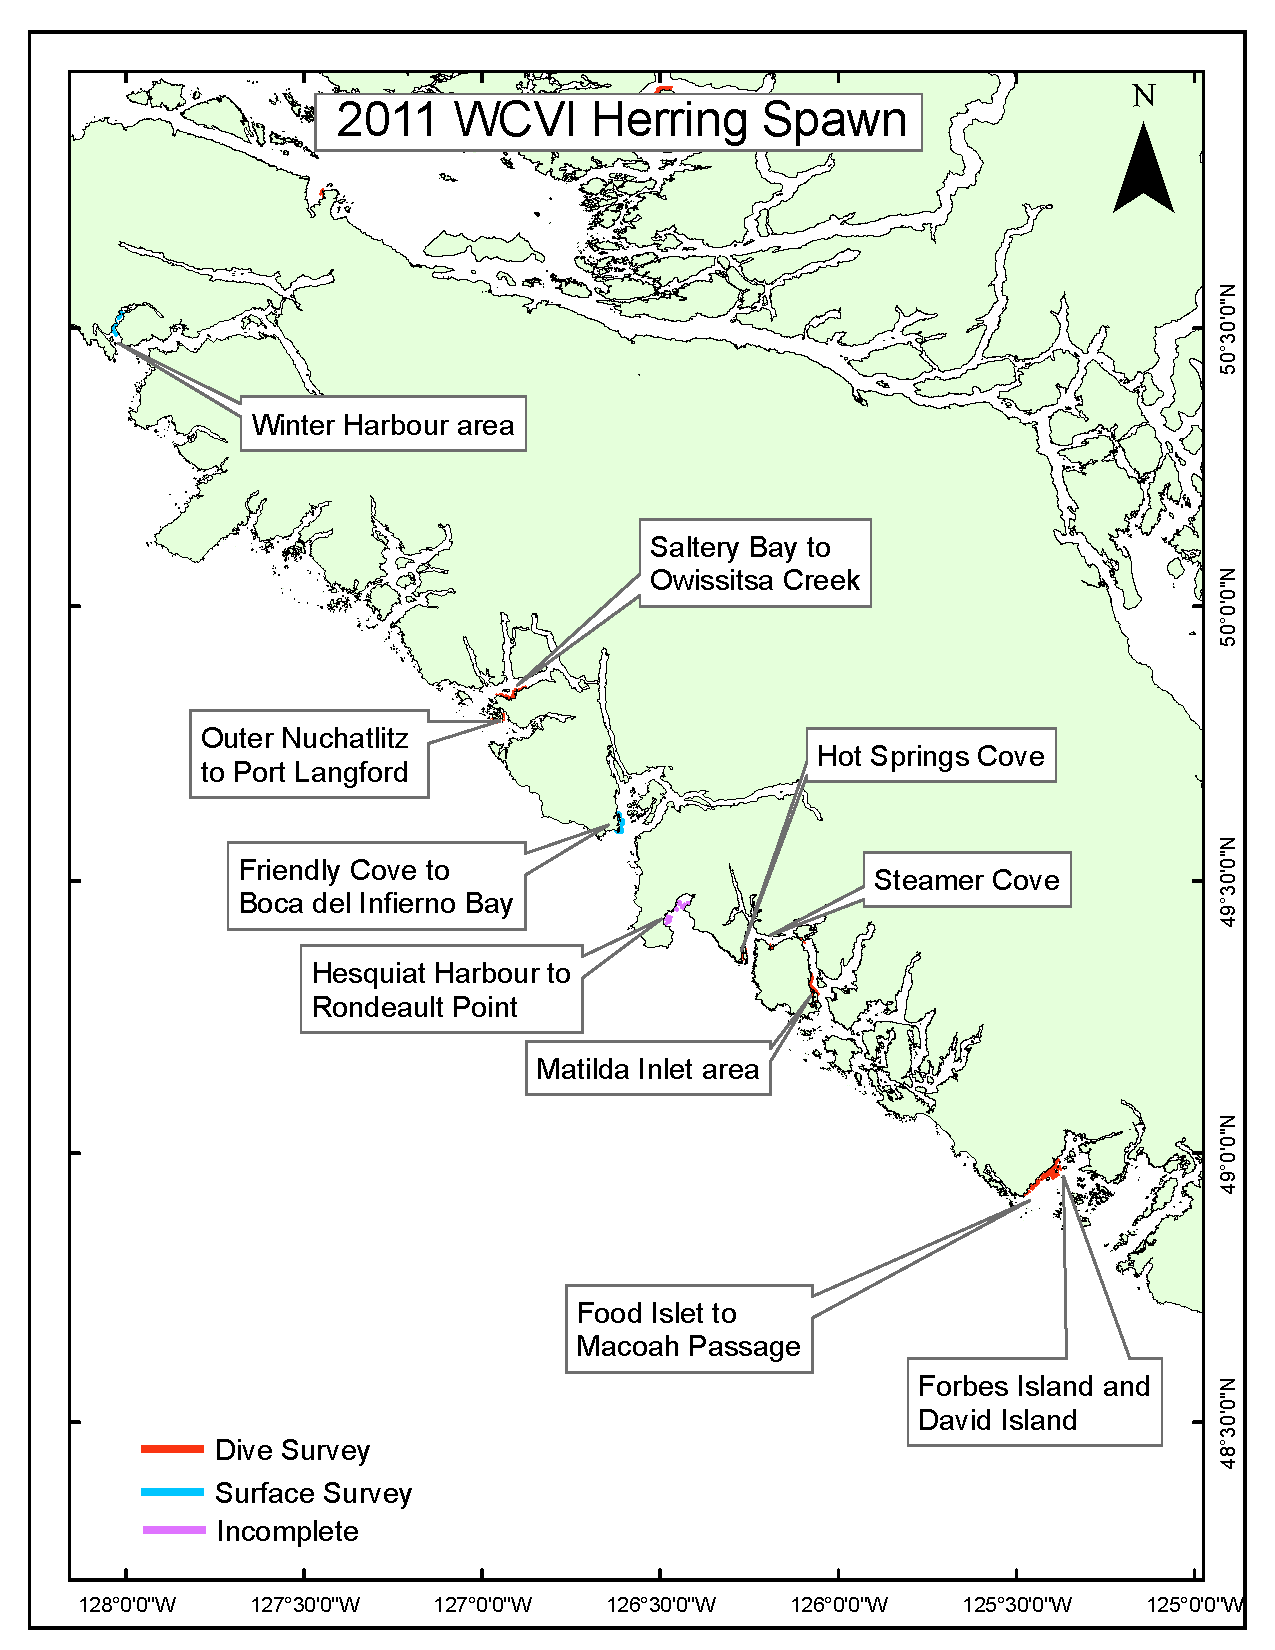
\includegraphics[scale=0.35]{../Figs/PBSfigs/2011_spawn_WCVI_August16.pdf}
	\caption{Preliminary Spawning activity for Central Coast (top left panel), Strait of Georgia (top right) in 2011 and west coast Vancouver Island (bottom).}\label{figSpawnMaps}
\end{figure}
% \begin{figure}[!tbp]
% 	% Requires \usepackage{graphicx}
% 	\ContinuedFloat
% 	\centering
% 	%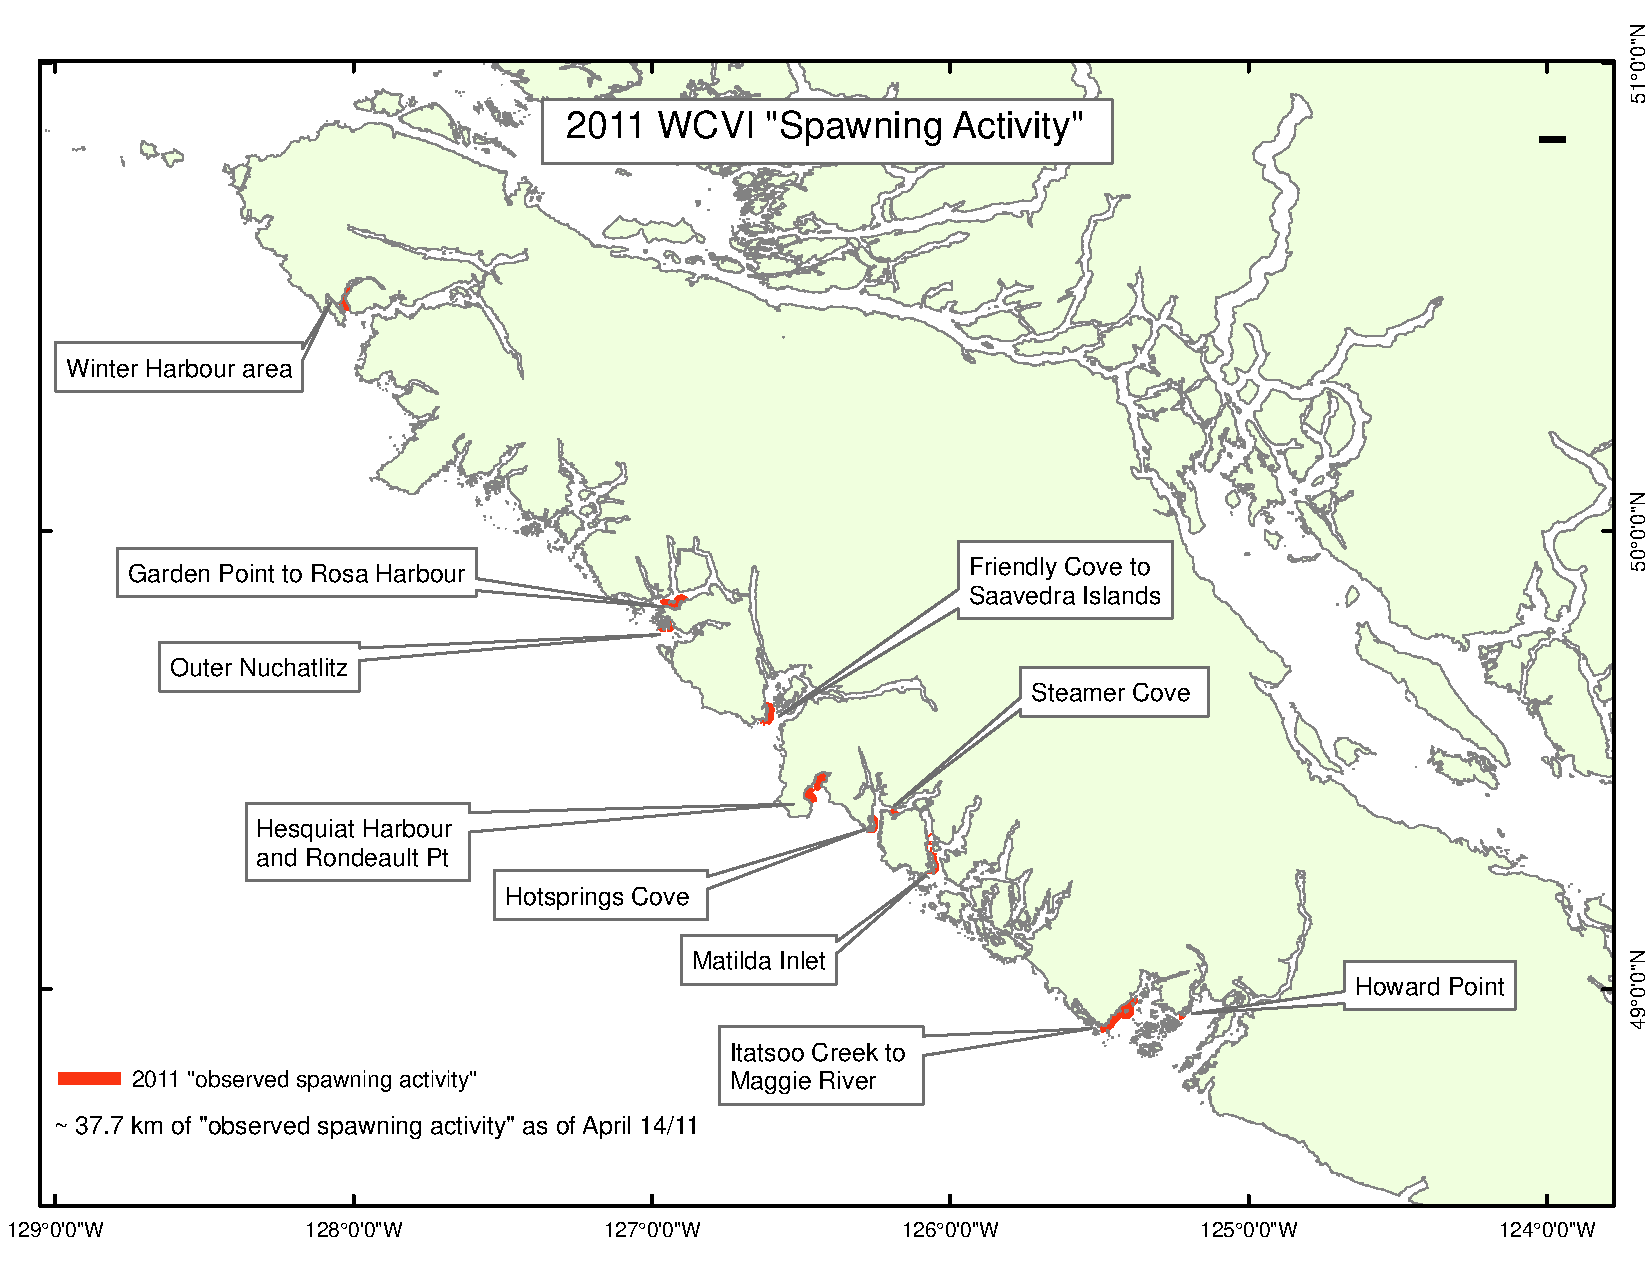
\includegraphics[scale=0.5]{../Figs/PBSfigs/2011-WCVI-Prelim-WG.pdf}\\
% 	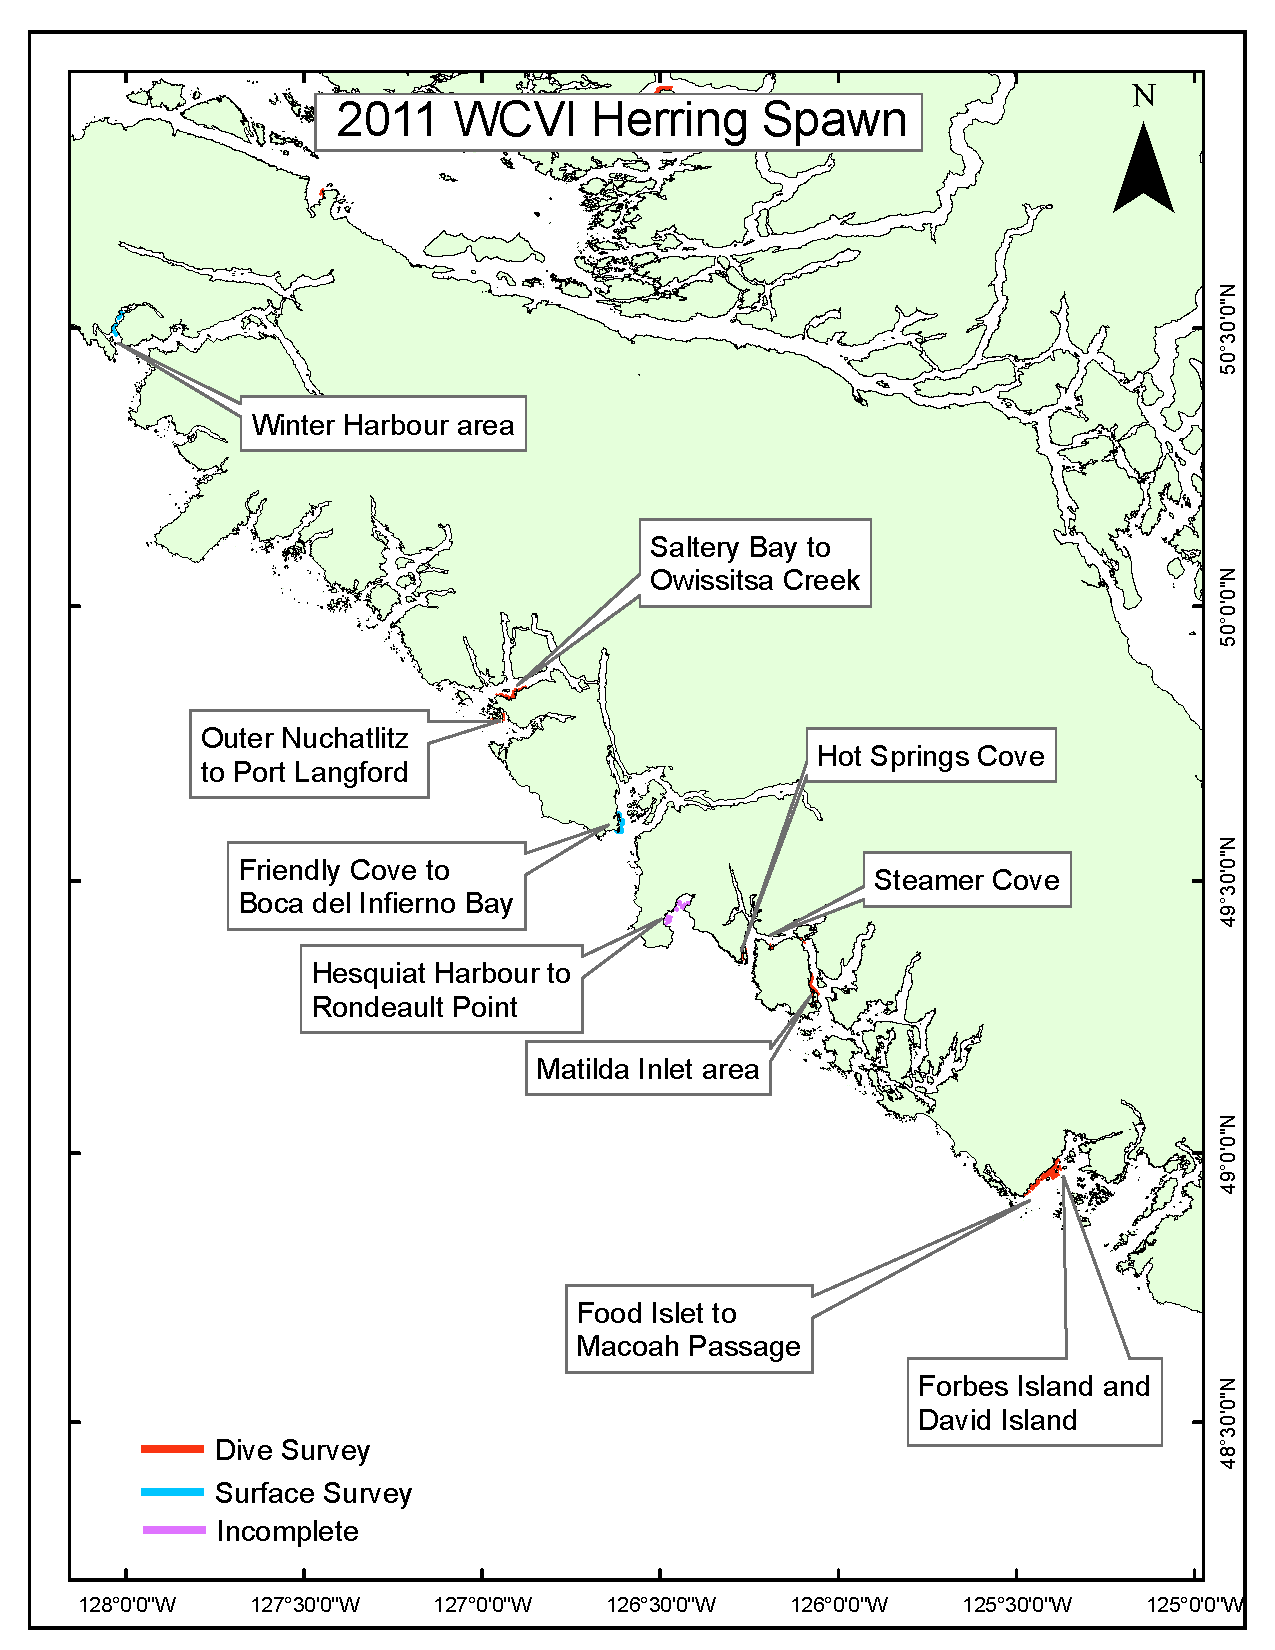
\includegraphics[scale=0.5]{../Figs/PBSfigs/2011_spawn_WCVI_August16.pdf}\\
% 	\caption{Preliminary Spawning activity in 2011 for the West Coast of Vancouver Island (includes minor stock area 27).}\label{figSpawnMaps}
% \end{figure}

	The spawn survey is conducted after the fisheries in the area have been completed; therefore, it is assumed that all the mortality for the year has occurred just prior to commencing the spawning survey. The fisheries independent survey estimates egg density and total spawn area, and from this information the total female spawning biomass can be estimated assuming the 200 eggs per gram of female  or 100 eggs per gram of mature  individuals \citep{hay1985reproductive,hardwick1973biomass}. The assumed selectivity for the spawn survey is fixed to the maturity schedule for herring.  	
	
\begin{figure}[!tbp]
	% Requires \usepackage{graphicx}
	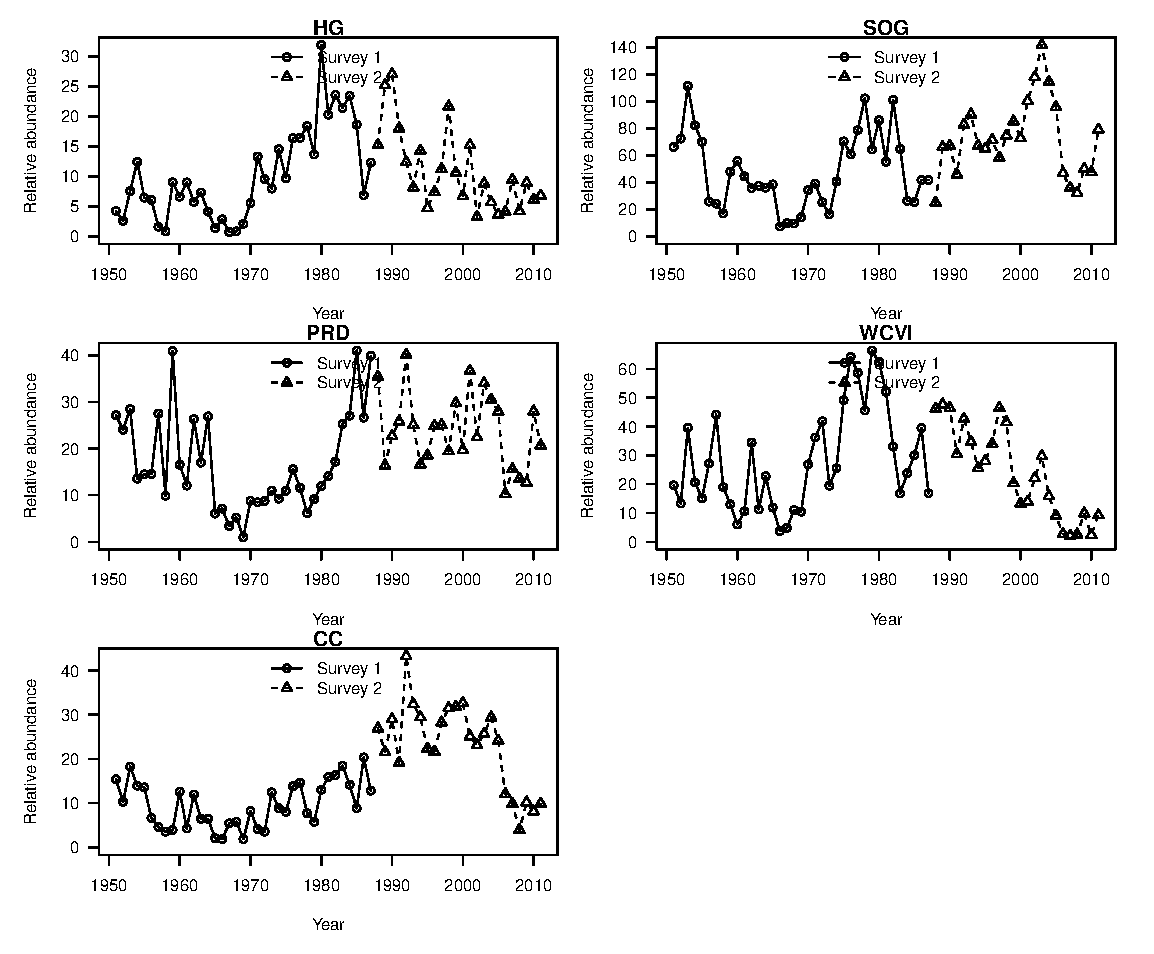
\includegraphics[width=\textwidth]{../Figs/iscam_fig_SurveyMajorAreas.pdf}\\
	\caption{Spawn survey index for Strait of Georgia between 1951 and 2011. The units are actual estimates of spawning biomass (1000s tons), but only the trend information is used in the model fitting.}\label{FigSurvey}
\end{figure}
	
	\subsubsection{Biological samples}
	
	Biological samples are collected from both commercial catch and from the test fishery program.  Commencing  in 1975, test fishery charters supplemented biological samples in areas with poor sampling that was not representative of the stock in that area (i.e., fishing solely on spawning aggregations), or in closed areas. Prior to 2006, test fishing charters were funded through an allocation of fish to the test program; the program is now fully funded by DFO.  Through a contract with DFO, the Herring Conservation and Research Society (HCRS) sub-contracts a number of vessels to collect biological samples.  Industry also conducts pre-season test sets for roe-quality testing in open areas and supplementary biological samples are provided as part of this program.  The following data are collected for all biological samples: fish length, weight, sex, and maturity.  Subsequently these sources of data are combined and information on weight-at-age and proportion-at-age become input data for the stock assessment model.
	
	During the 2010/2011 season a total of 248 biological samples were collected, of which 151 were collected from the test fishery, 57 were collected from the roe fishery, 16 from the food \& bait fishery, 4 from Spawn on Kelp (SOK) operations, and 16 from the summer trawl research survey (Table \ref{table:PartII:bioSamples}).  Note that the definition of a sample is roughly 100 individual fish.  A summary of biological samples collected from commercial and pre-fishery charters from 2002/03--2010/11 is presented in Table \ref{table:PartII:sampleSizes}).

\begin{table}
	\caption{Summary of biological samples collected and processed from all sources from the 2010/11 herring season.}
	\label{table:PartII:bioSamples}
	\begin{center}
		\begin{tabular}{cccccc}
		\hline
		& \multicolumn{3}{c}{Commercial samples} &  \\
		Stock & Roe fishery & SOK fishery & F\&B & Test fishery & Research\\
		\hline
		HG (QCI 2E) &  &  &  & 13\\
		PRD & 29 & 1 &  & 24\\
		CC &  &  &  & 30\\
		SOG & 18 &  & 20 & 60\\
		WCVI &  &  &  & 14 & 16\\
		Area 2W &  &  &  & 10\\
		Area 27 &  & 3\\
		Other Areas\\
		\hline
		Total & 57 & 4 & 16 & 151 & 16\\
		\hline
		\end{tabular}
	\end{center}
\end{table}

\begin{table}
	\caption{Summary of biological samples collected and processed from commercial catch and test fishery charters from 2002/03-2010/11.}
	\label{table:PartII:sampleSizes}
	\begin{center}
\begin{tabular}{cccc}
\hline
Fishing season & Commercial fishery samples & Charter and research samples & Total\\
\hline
2002/03 & 120 & 287 & 407\\
2003/04 & 79 & 222 & 301\\
2004/052 & 83 & 191 & 274\\
2005/06 & 46 & 164 & 210\\
2006/07 & 114 & 85 & 199\\
2007/08 & 116 & 103 & 219\\
2008/09 & 87 & 136 & 223\\
2009/10 & 78 & 135 & 213\\
2010/11 & 81 & 167 & 248\\
\hline
\end{tabular}
	
	\end{center}
\end{table}
	
	
	
	%%Insert Summary of biological samples from the 2010/2011 season here:
	
	%%Insert Summary of biological samples collected and processeed from commercial catch etc. here (Table 2 from Cleary 2011).
	
	\subsubsection{Age composition data}
	
	Ageing data, through the reading of fish scales, are collected from the biological samples taken from the commercial fisheries and test fishery charters. Age composition data is used to determine proportions-at-age and is an essential source of input data to the herring stock assessment model.
	
	Catch-at-age data from the winter seine fishery (top panels of Figures \ref{FigAgeCompsHG}-\ref{FigAgeCompsWCVI}) tend to consist of younger fish in comparison to the age composition data from the seine-roe and gillnet fleets post 1970. The shaded polygons in Figures \ref{FigAgeCompsHG}-\ref{FigAgeCompsWCVI} approximates the 95\% distribution of ages in the catch.  Roughly 90\% of the fish landed in the winter seine fishery were younger than age-7, and younger than age-6 in recent years.  In both the winter seine and seine-roe fishery age-2 fish are frequently landed; whereas, age-2 fish are rarely landed in the gillnet fishery, and fish do not appear to fully recruit to the gear until at least 4-5 years of age.  The mean age of the catch appears to be increasing between 2008 and 2010 in both the gillnet and winter seine fishery, and there is no obvious trend in the seine roe fishery.  There is however a declining trend in the older ages caught in the seine-roe fishery since 2006 (erosion of age-structure).

\begin{sidewaysfigure}[!tbp]
	% Requires \usepackage{graphicx}
	\centering
	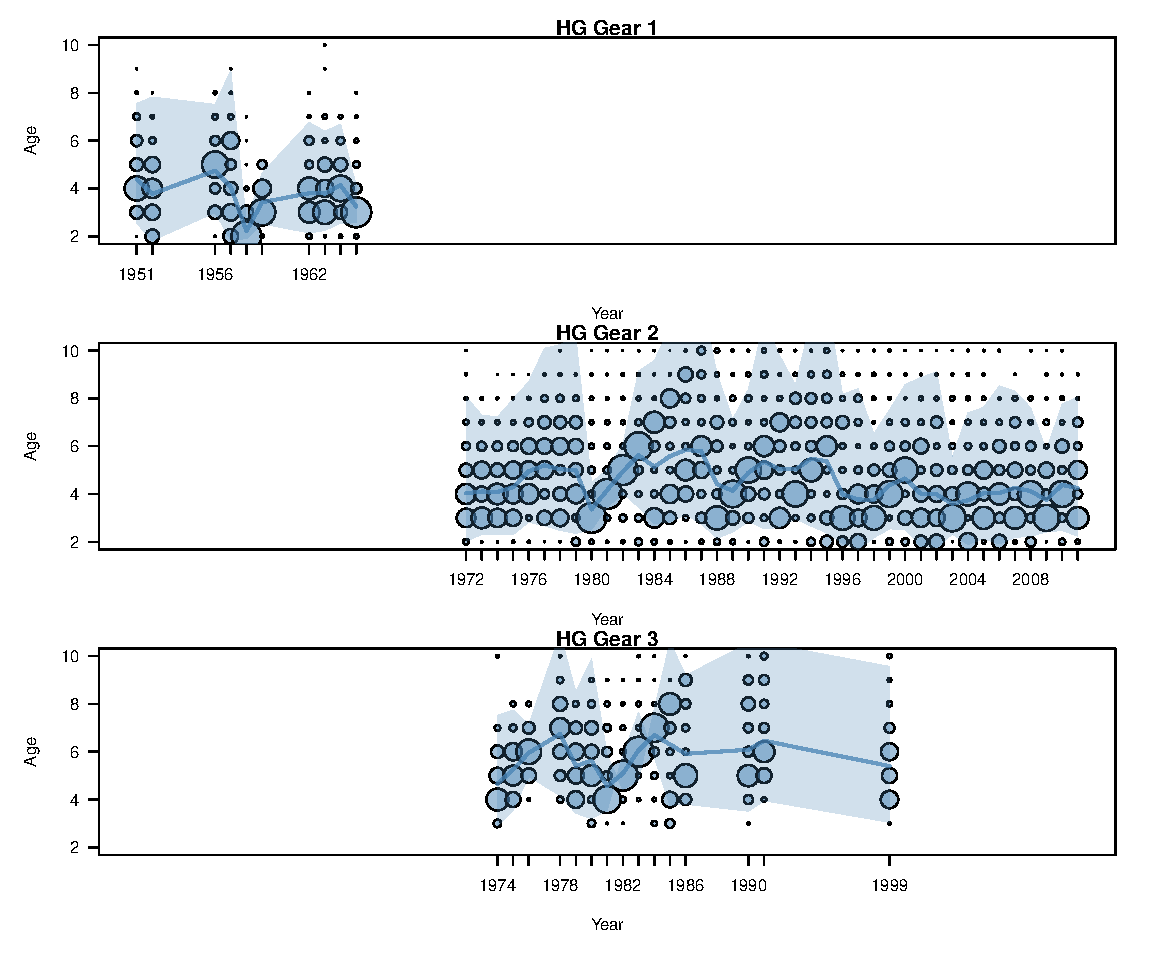
\includegraphics[width=0.85\textwidth]{../Figs/iscam_fig_AgeCompsHG.pdf}\\
	\caption{Bubble plots showing the proportions-at-age versus time for the winter purse seine fishery (top), seine roe fishery (middle) and the gillnet fishery (bottom) in Haida Gwaii.  The area of the circle is proportional to cohort abundance, each column sums to 1, zeros are not shown, and age 10 is a plus group. Also shown is the mean age of the catch (line) and the approximate 95\% distribution of ages (shaded polygon) for each year.}\label{FigAgeCompsHG}
\end{sidewaysfigure}

\begin{sidewaysfigure}[!tbp]
	% Requires \usepackage{graphicx}
	\centering
	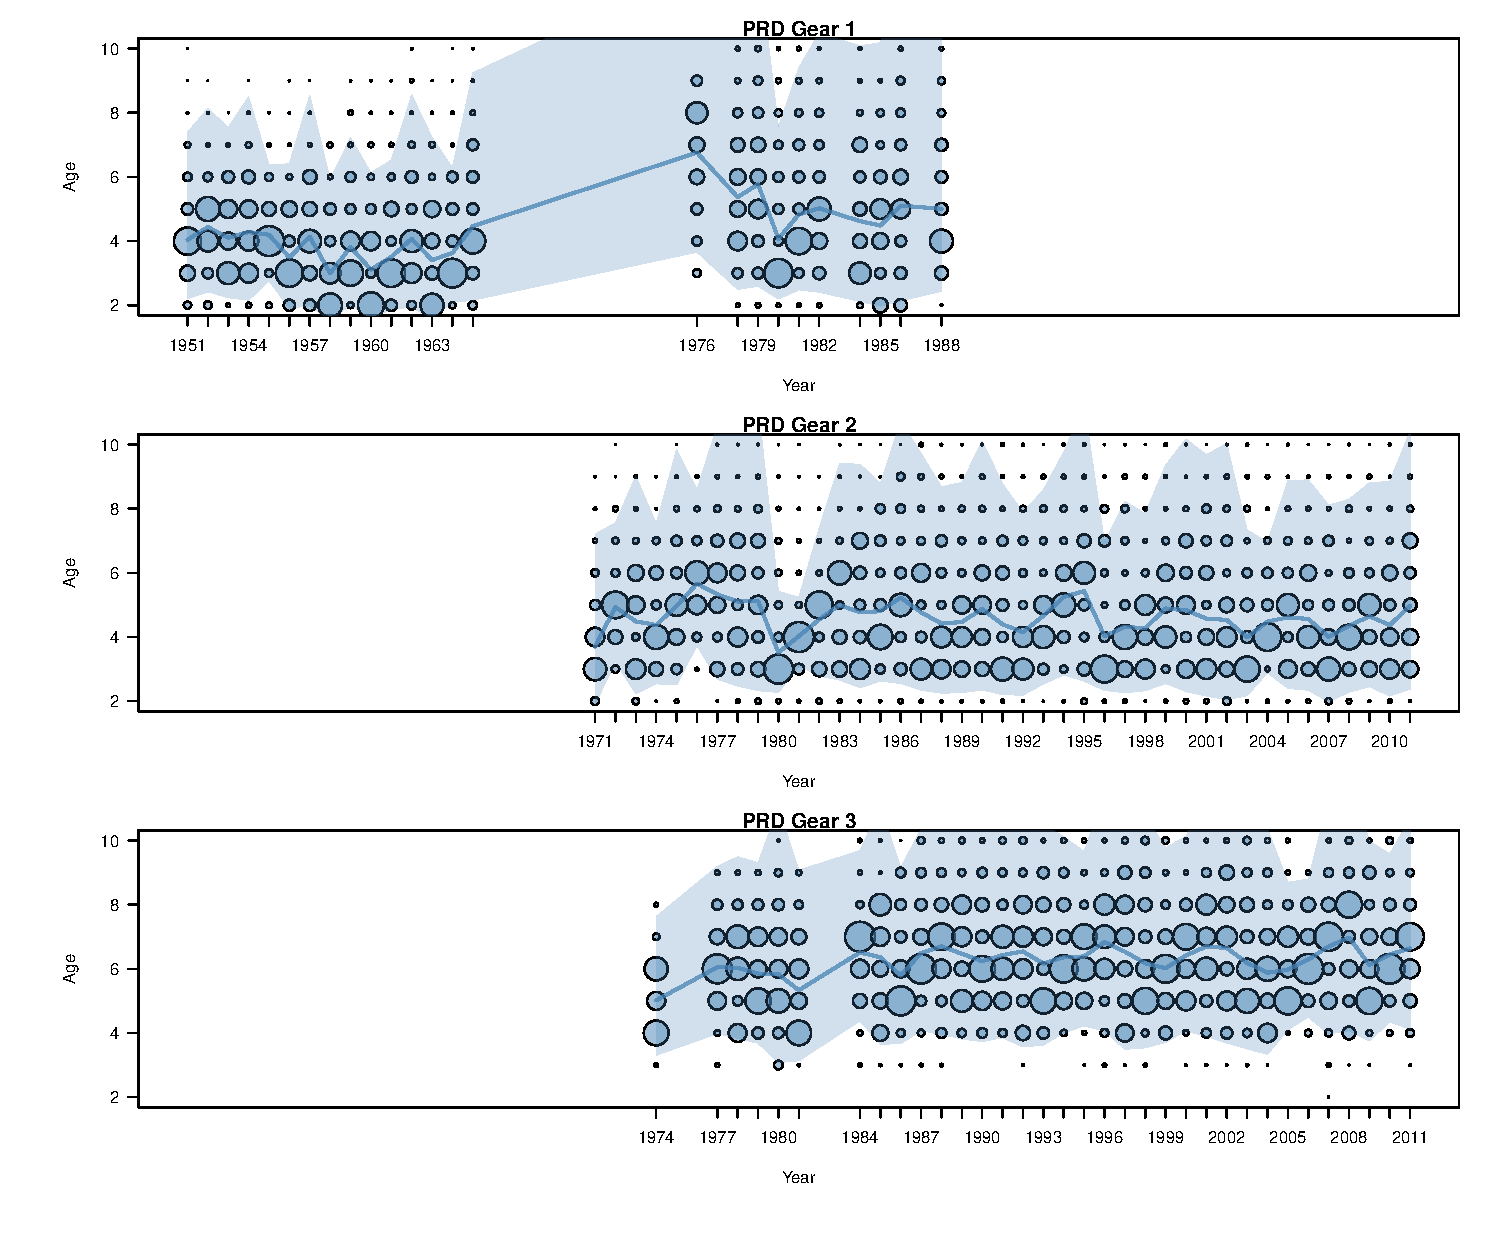
\includegraphics[width=0.85\textwidth]{../Figs/iscam_fig_AgeCompsPRD.pdf}\\
	\caption{Bubble plots showing the proportions-at-age versus time for the winter purse seine fishery (top), seine roe fishery (middle) and the gillnet fishery (bottom) in Prince Rupert District.  The area of the circle is proportional to cohort abundance, each column sums to 1, zeros are not shown, and age 10 is a plus group. Also shown is the mean age of the catch (line) and the approximate 95\% distribution of ages (shaded polygon) for each year.}\label{FigAgeCompsPRD}
\end{sidewaysfigure}

\begin{sidewaysfigure}[!tbp]
	% Requires \usepackage{graphicx}
	\centering
	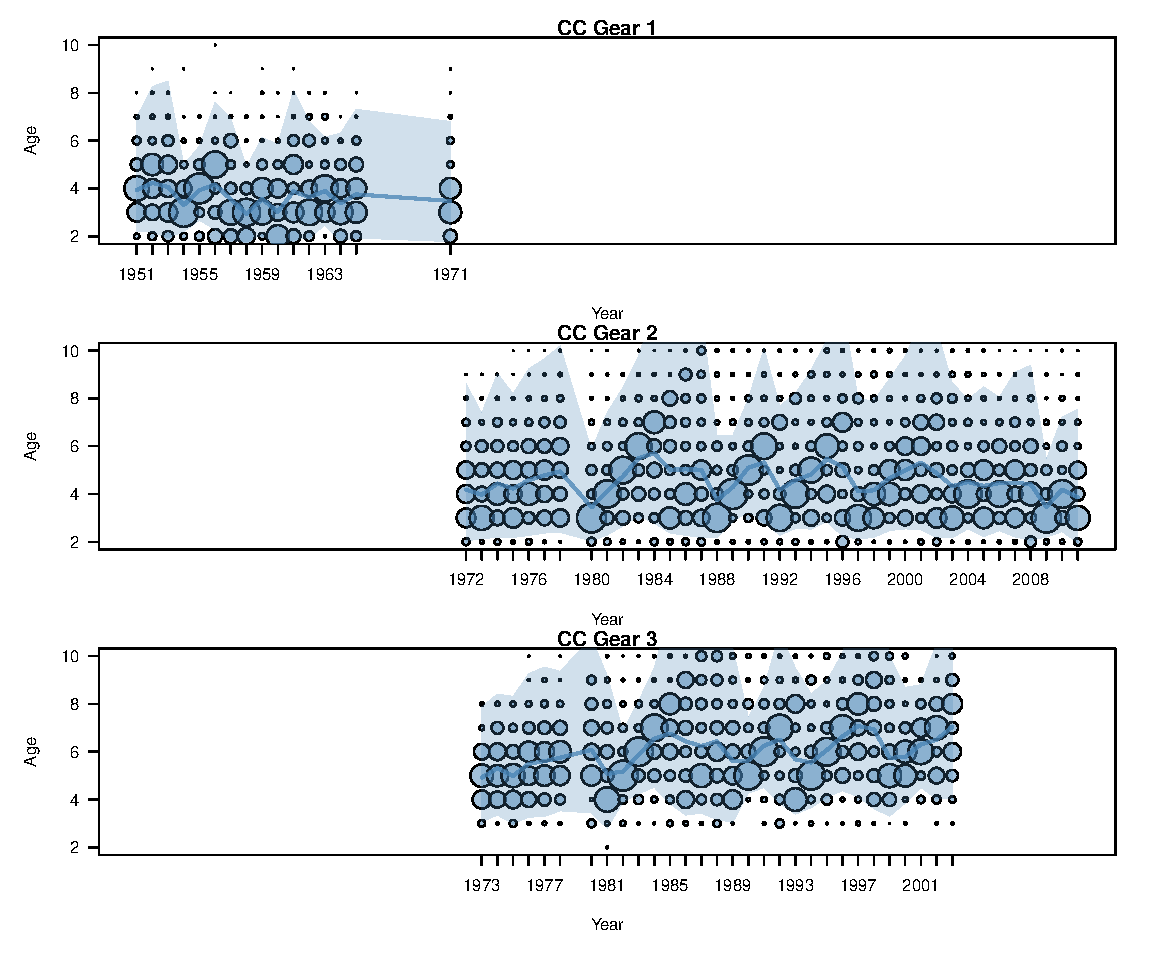
\includegraphics[width=0.85\textwidth]{../Figs/iscam_fig_AgeCompsCC.pdf}\\
	\caption{Bubble plots showing the proportions-at-age versus time for the winter purse seine fishery (top), seine roe fishery (middle) and the gillnet fishery (bottom) in the Central Coast region.  The area of the circle is proportional to cohort abundance, each column sums to 1, zeros are not shown, and age 10 is a plus group. Also shown is the mean age of the catch (line) and the approximate 95\% distribution of ages (shaded polygon) for each year.}\label{FigAgeCompsCC}
\end{sidewaysfigure}

\begin{sidewaysfigure}[!tbp]
	% Requires \usepackage{graphicx}
	\centering
	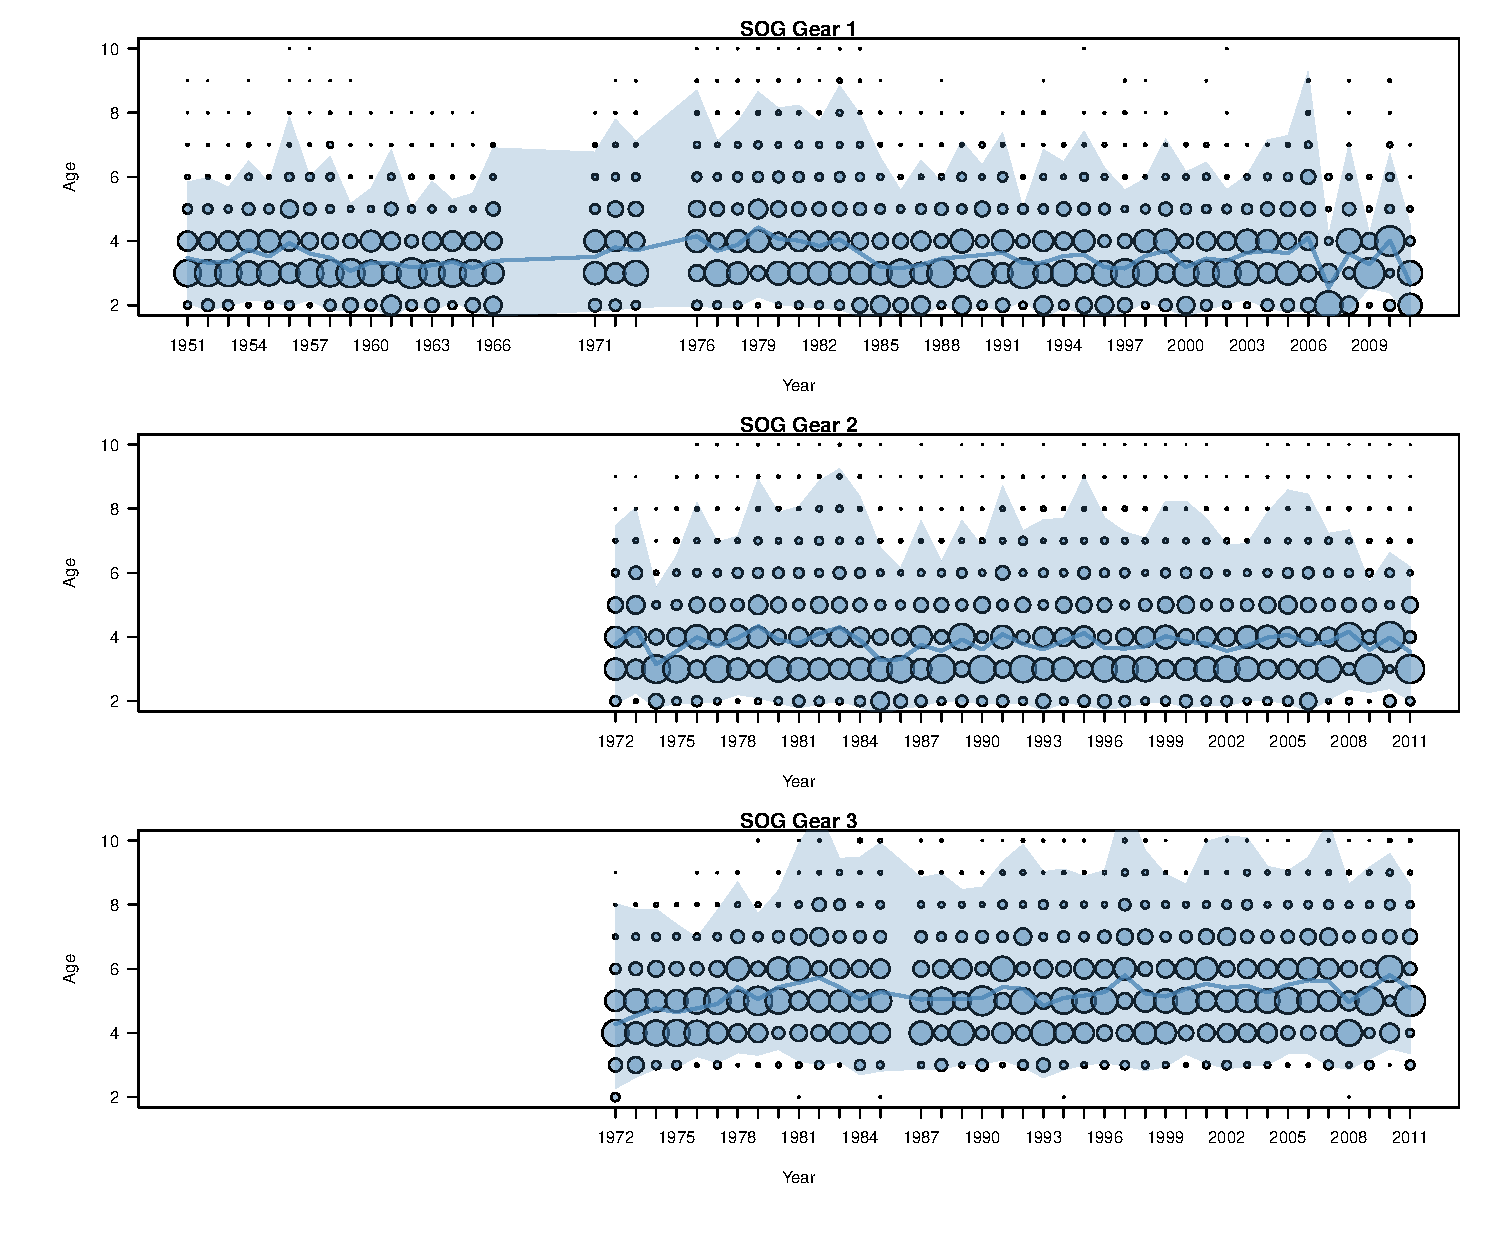
\includegraphics[width=0.85\textwidth]{../Figs/iscam_fig_AgeCompsSOG.pdf}\\
	\caption{Bubble plots showing the proportions-at-age versus time for the winter purse seine fishery (top), seine roe fishery (middle) and the gillnet fishery (bottom) in the Strait of Georgia.  The area of the circle is proportional to cohort abundance, each column sums to 1, zeros are not shown, and age 10 is a plus group. Also shown is the mean age of the catch (line) and the approximate 95\% distribution of ages (shaded polygon) for each year.}\label{FigAgeCompsSOG}
\end{sidewaysfigure}

\begin{sidewaysfigure}[!tbp]
	% Requires \usepackage{graphicx}
	\centering
	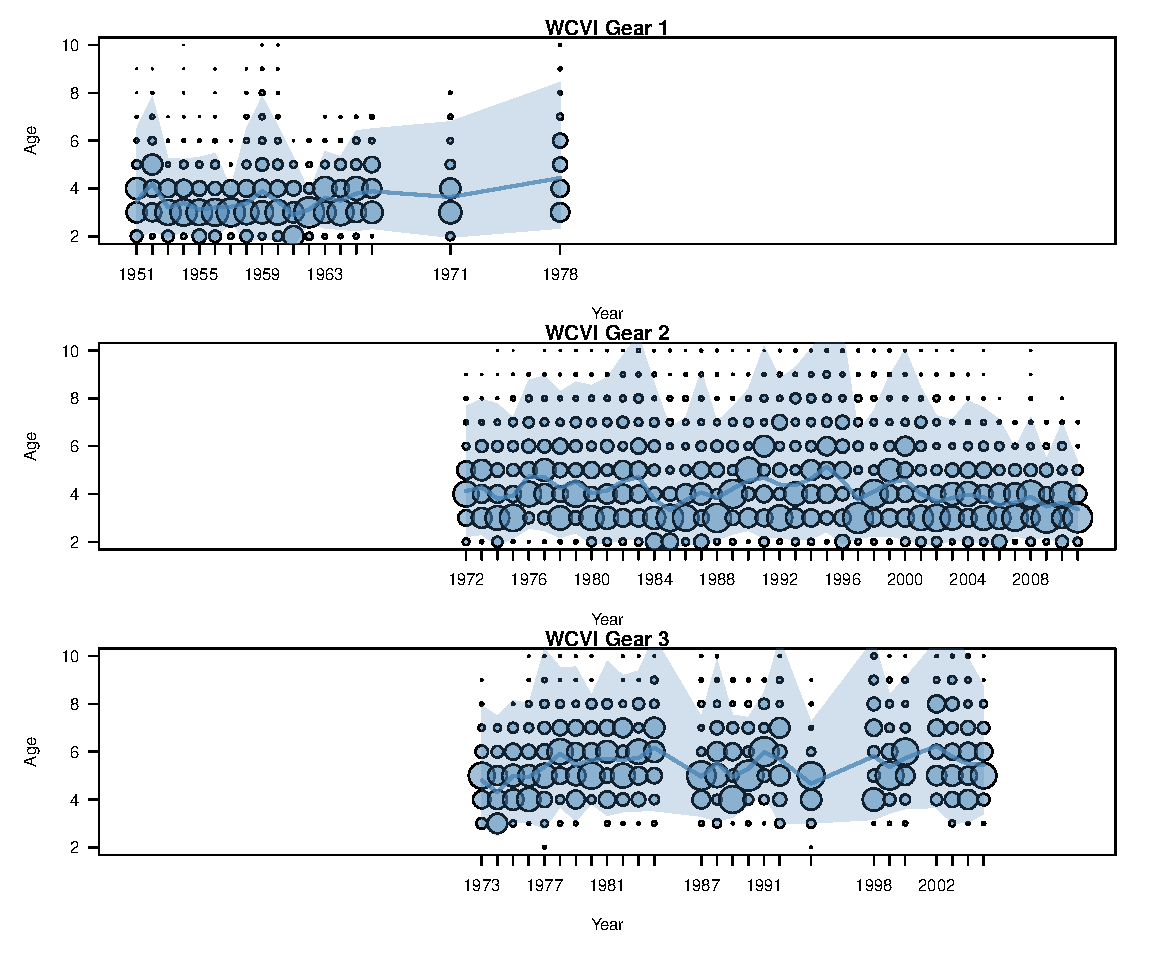
\includegraphics[width=0.85\textwidth]{../Figs/iscam_fig_AgeCompsWCVI.pdf}\\
	\caption{Bubble plots showing the proportions-at-age versus time for the winter purse seine fishery (top), seine roe fishery (middle) and the gillnet fishery (bottom) in the West Coast Vancouver Island region.  The area of the circle is proportional to cohort abundance, each column sums to 1, zeros are not shown, and age 10 is a plus group. Also shown is the mean age of the catch (line) and the approximate 95\% distribution of ages (shaded polygon) for each year.}\label{FigAgeCompsWCVI}
\end{sidewaysfigure}





	\subsubsection{Mean weight-at-age data}

	From the mid-1970s until the present, there has been a measurable decline in weight-at-age for all ages in all major stock areas (Figure \ref{FigMeanWt}). Samples collected during the 2009/10 fishing year indicate weights-at-age that are among the lowest on record. This declining weight-at-age may be attributed to any number of factors, including: fishing effects (i.e., gear selectivity), environmental effects (changes in ocean productivity), or it may even be attributed to changes in sampling protocols (shorter time frame over which samples are collected). Declining weight-at-age has been observed in all five of the major stocks, and despite area closures over the last 10-years, has continued to occur in the QCI and WCVI stocks. Although the direct cause of this decline is still to be investigated, this trend has been observed in B.C. and U.S. waters, from California to Alaska \citep{schweigert2002herring}, and merits further research.	The observed mean weight-at-age data appear to have a few  errors that need to be investigated as well; for example, see the apparently small age-10 fish in 2001 in Figure \ref{FigMeanWt}.

\begin{figure}[!tbp]
	% Requires \usepackage{graphicx}
	\centering
	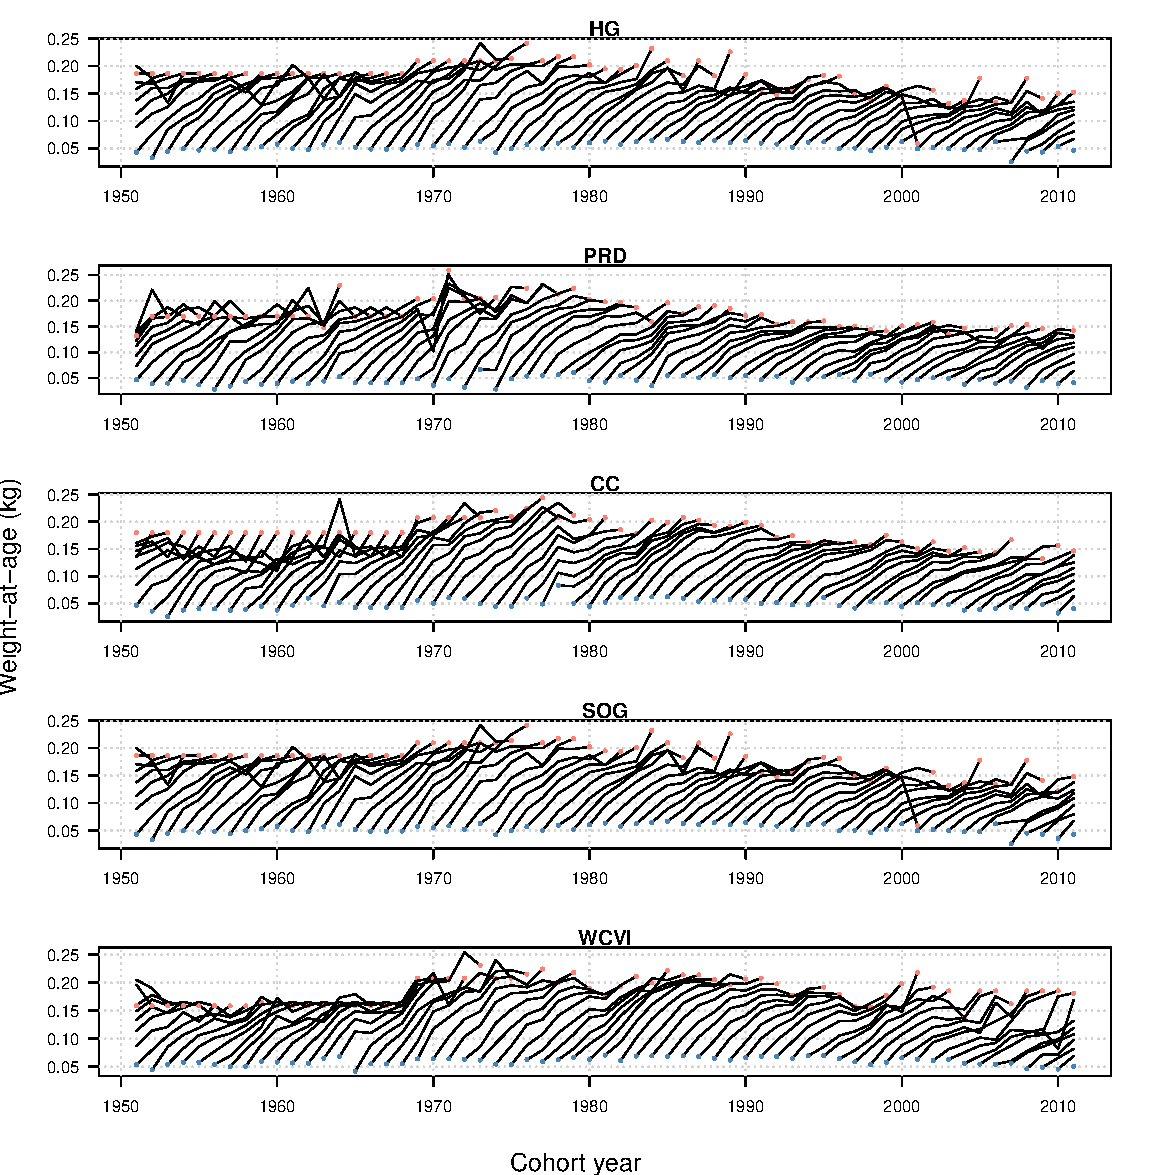
\includegraphics[width=\textwidth]{../Figs/iscam_fig_MeanWt.pdf}\\
	\caption{Empirical mean weight-at-age data by cohort from 1951 to 2011 for ages 2 to 10 in the five major Stock Assessment Regions.}\label{FigMeanWt}
\end{figure}
	

%%%%%%%%%%%%%%%%%%%%%%%%%%%%%%%%%%%%%%%%%%%%%%%%%%%%%%%%%%%%%%%%%%%%%
%%%%%%%%%%%%%%%%%%%%%%%%%%%%%%%%%%%%%%%%%%%%%%%%%%%%%%%%%%%%%%%%%%%%%
%%%%%%%%%%%%%%%%%%%%%%%%%%%%%%%%%%%%%%%%%%%%%%%%%%%%%%%%%%%%%%%%%%%%%	
	\subsection{Analytical methods}

	For the 2011 BC herring assessment, \iscam was used to conduct the stock assessment for each of the five major Stock Assessment Regions (SAR) and two minor assessment areas (Area 2W and Area 27).  The technical details of this model can be found in Appendix \ref{appiSCAM}.
		
	\subsection{Retrospective analysis}
	A retrospective analysis was conducted for each of the major and minor SARs.  The retrospective analysis successively removes the last 10-years of data and examines changes in estimates of terminal spawning biomass.  The results are then plotted on a single panel to compare how estimates of spawning biomass change as successive years of data are omitted from the analysis.
	
	\subsection{Abundance and recruitment forecasts}
	The abundance forecast for the upcoming fishing season, also referred to as pre-fishery biomass, is defined as the predicted biomass of age-4 fish and older plus the number of age-3 fish recruiting in year $T+1$.  The abundance estimates are based on the median values from the sampled posterior distribution.  Age-3 recruits are based on poor, average, and good recruitment scenarios; see next paragraph for definitions of poor, average and good.
	
	The recruitment forecasts are based on the surviving number of age-3 fish at the start of the fishing season times the average weight-at-age 3 in the last 5 years. The definitions of poor, average, and good recruitment are as follows: \textbf{Poor} is the average recruitment from the 0-33 percentile, \textbf{Average} is the average recruitment from the 33-66 percentile, and \textbf{Good} is the average recruitment from the 66-100 percentile.  Note that all cohorts from 1951 to 2011  were included in the calculation of recruitment quantiles.
	
	\subsection{Catch advice}
Catch advice is based on the application of the harvest control rule (HCR). The herring HCR has three components:
\begin{enumerate}
\item Reference points (LRP, USR, and cuttoffs)
\item Harvest rate
\item Decision rules
\end{enumerate}

For each of the five major stocks, the limit reference point (LRP) is the cuttoff value, which is defined here as 0.25\bo\, and the	Upper Stock Reference (USR) is defined as the 1.05*LRP (0.25\bo\ + 0.2*0.25\bo = LRP + 0.05LRP). \textbf{For clarification, references to \bo\ throughout this document refer to the mature spawning stock biomass.} The default harvest rate if the stock is at or above USR is 0.2, and declines linearly to 0 when the stock is at or below the LRP (a default harvest rate of 0.1 is used for the minor stock areas).  The decision rule for the major stock areas operates as follows:

\begin{itemize}
	\item If the forecast run is less than the LRP (cuttoff) then the area is closed to all commercial harvest  (i.e., stock is deemed to be in the critical zone).
	
	\item If the forecast run is greater than the LRP and less than the USR (i.e., cautious zone), then total allowable catch is based on a reduced harvest rate that would deplete the stock to the LRP level.
	
	\item If the forecast run is greater than USR, then the total allowable catch is set at 20\% of the forecast run.
\end{itemize}



	



%!TEX root = /Users/stevenmartell/Documents/CURRENT PROJECTS/iSCAM-trunk/fba/BC-herring-2011/WRITEUP/BCHerring2011.tex


\part{Stock Assessment and Management Advice for the British Columbia Pacific Herring Stocks: 2011 Assessment and 2012 Forecasts}

\addtocounter{chapter}{1}

%% SECTION Introduction
\section{Introduction}
	
There are four major objectives of this paper: (1) to describe in detail an alternative integrated statistical catch-age model (iSCAM), (2) examine parameter estimation performance using iSCAM, (3) perform a side-by-side comparison of the previous HCAM and iSCAM on the five major herring stocks, and (4) explore alternative assumptions about selectivity, catchability, and natural mortality using iSCAM.  The most recent assessment of BC herring stocks was conducted in 2010 using the Herring Catch Age Model (HCAMv2) which is documented in \cite{Clear2010}.  Furthermore, a review sponsored by the Herring Research and Conservation Society (HRCS) was conducted June 17-18, 2010 in Nanaimo, BC where an expert panel addressed specific questions about the current implementation of the HCAMv2 model and suggested recommendations for each of the questions.  This paper also attempts to address some of the points brought up in the review.

BC herring are currently managed as five major stocks and 2 minor stocks (Figure \ref{Fig1}).  Annual catch advice for each of these areas is based on current estimates of stock status, and a 20\% exploitation rate if the stock is above the cutoff level for the five major stocks and a 10\% exploitation rate for the two minor stocks.  Cutoff levels for the five major stocks are based on 0.25$B_o$, and estimates of unfished biomass were established first in 1985 \citep{haist1986stock}.  These cutoffs are currently are thought to be more conservative 	than the current default Limit Reference Point of 0.4\bmsy\ \citep{dfo2006}. However, estimates of $B_o$ and MSY based reference points have not been examined for Pacific herring for some time.  In this paper we also describe the methods for updating estimates of $B_o$ and MSY based reference points using the iSCAM model framework.  We also compare estimates of MSY based reference points for the Strait of Georgia herring under the previously mentioned alternative assumptions (see point (4) in the previous paragraph).

We do not provide a detailed description of HCAMv2 in this paper and we refer the reader to \cite{schweigert2009stock} and \cite{Clear2010} for a more detailed description.  We first begin with a description of the input data required and assumptions about the data, followed by a detailed description of the analytical methods and assumptions in iSCAM. We then present the analytical methods and assumptions for exploring alternative hypotheses about selectivity, catchability and natural mortality, followed by a description of the elements that make up the joint posterior distribution (i.e., likelihoods, priors, and penalties).  Parameter estimating and quantifying uncertainty is carried out using AD Model Builder \citep{ADMB2009}.  We then explore estimation performance in iSCAM using simulation experiments where the model is used to generate simulated observations with known parameter values, then estimate parameter, and repeat this exercise a number of times to evaluate bias and precision in parameter estimates.  Finally, we present forecast of pre-fishery biomass and available harvest options using the cutoffs \cite[e.g., reproduce Table 5 in ][]{Clear2010} as well as available harvest options based on the Sustainable Fisheries Framework \citep[i.e.,][]{dfo2006} for comparison.

\begin{figure}[!tbp]
	% Requires \usepackage{graphicx}
	%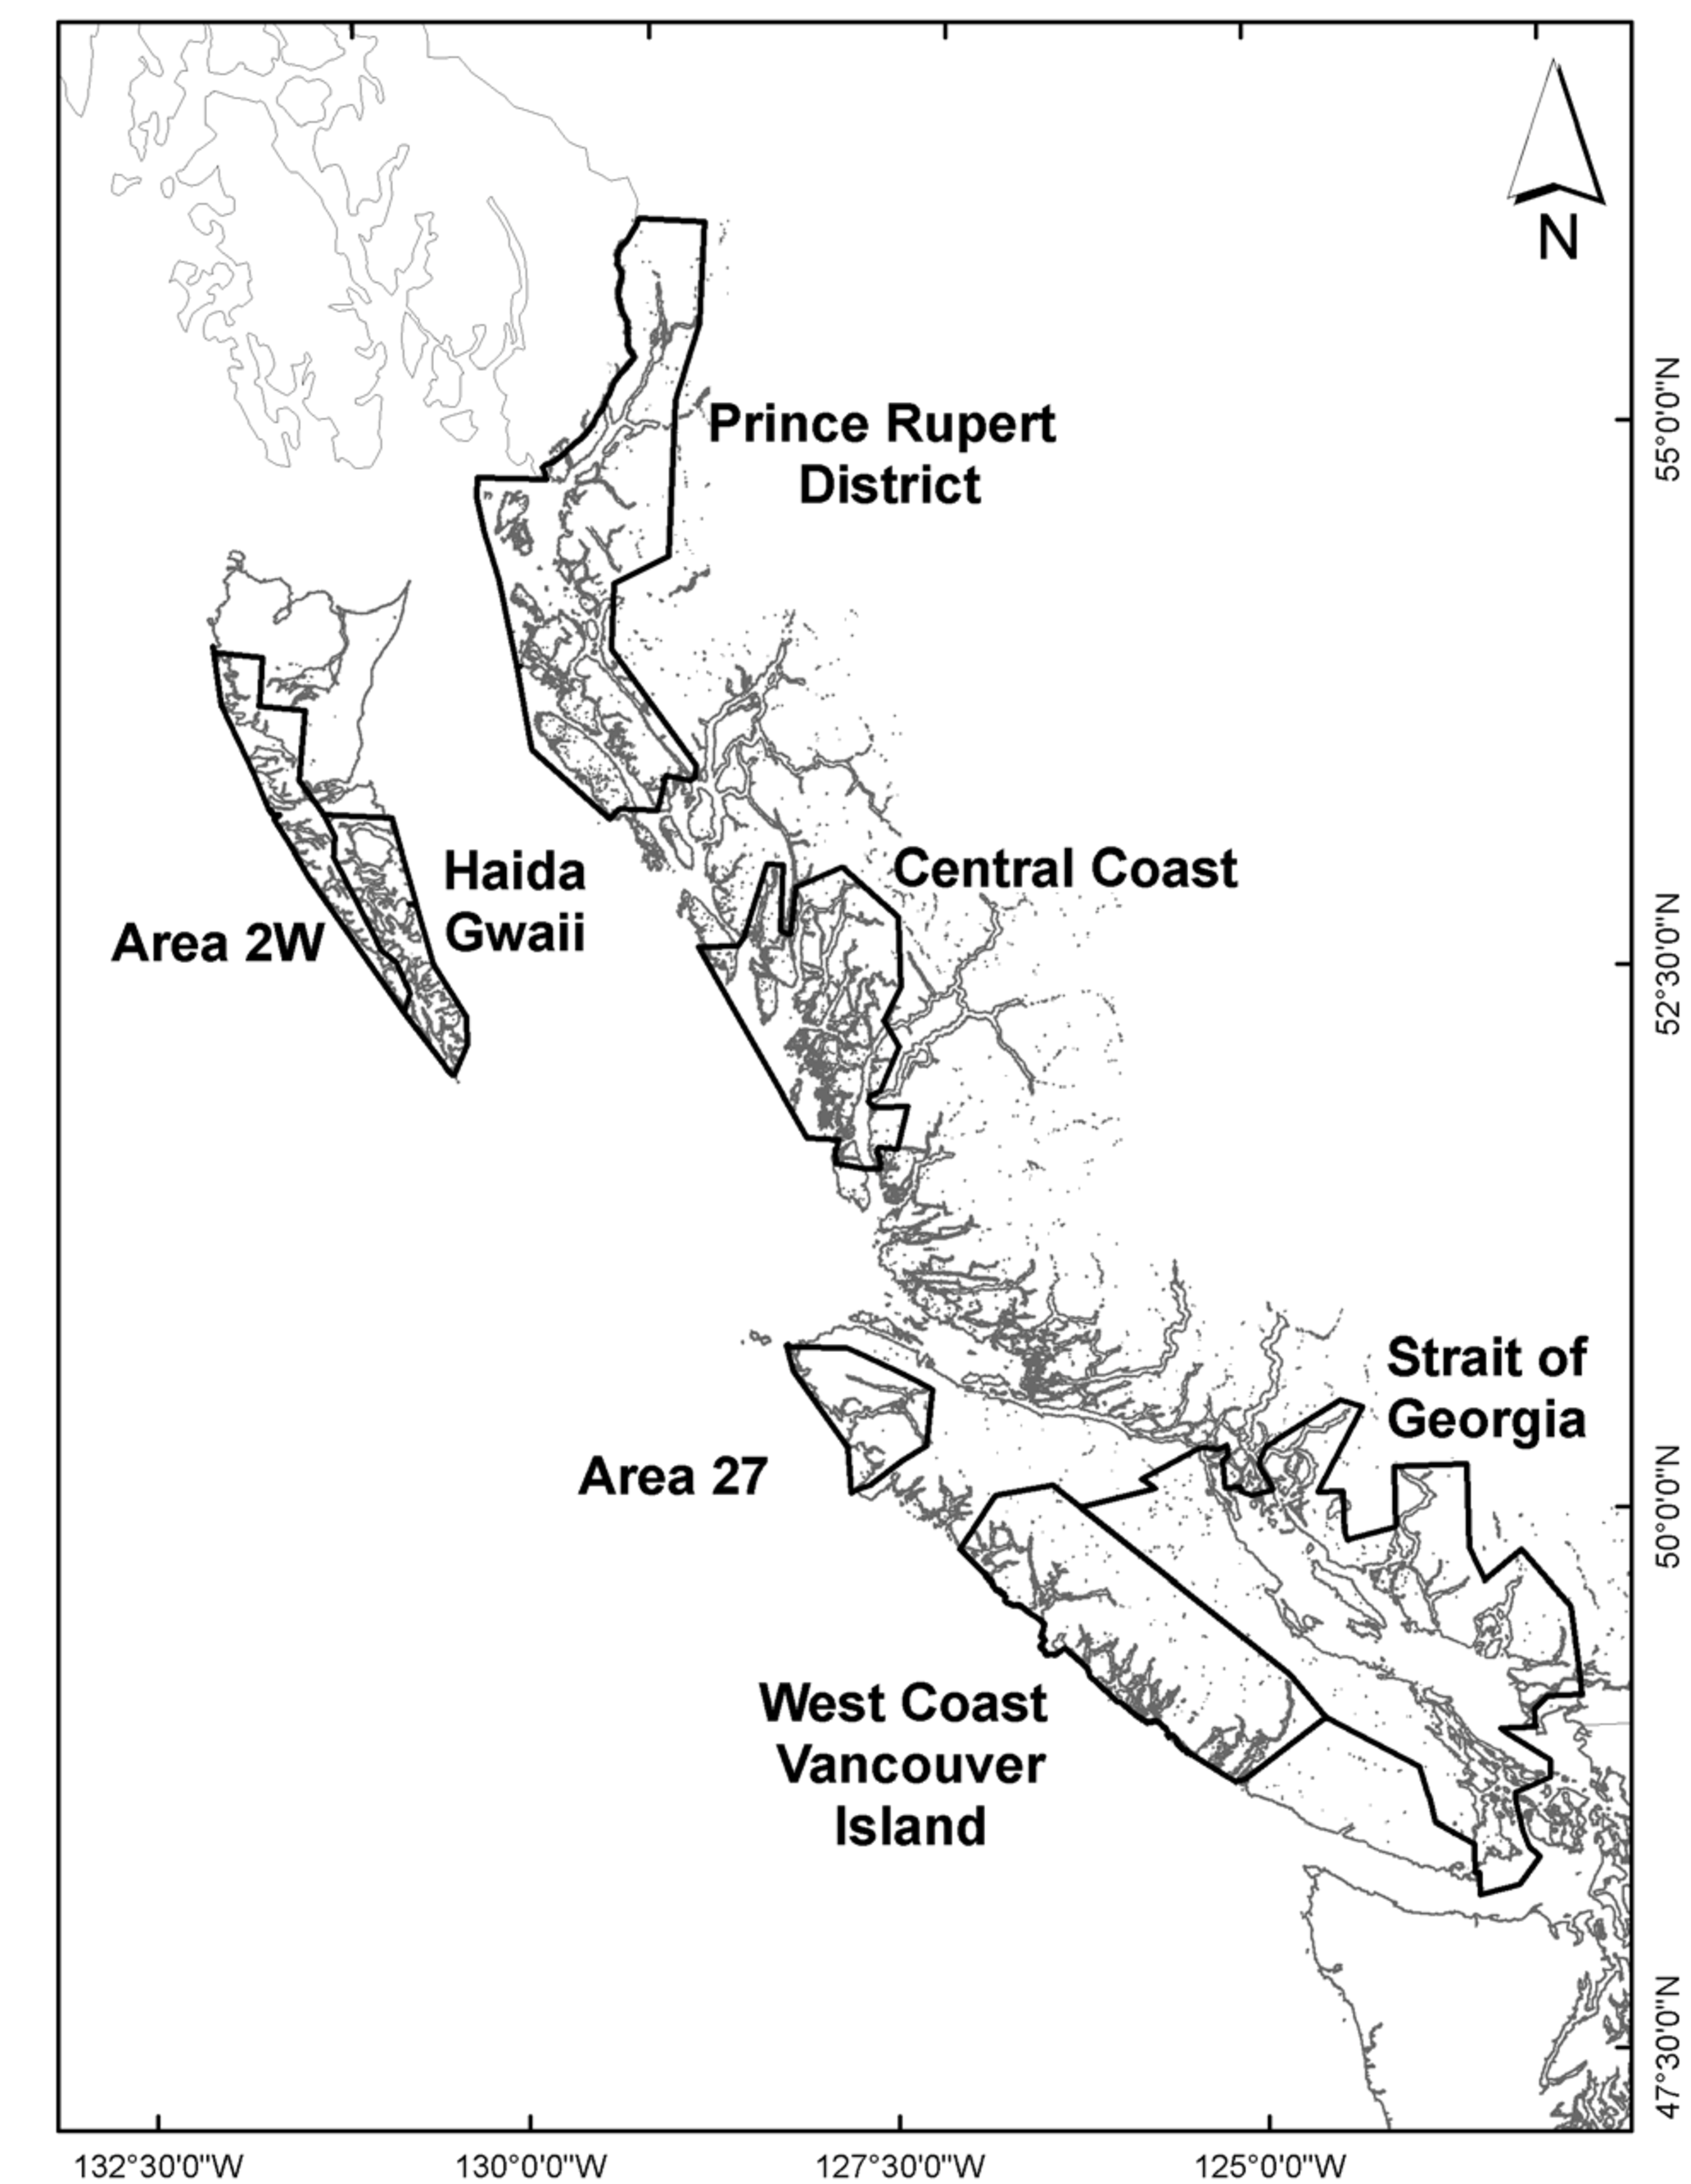
\includegraphics[width=\textwidth]{Figs/HerringAreaMap.pdf}
	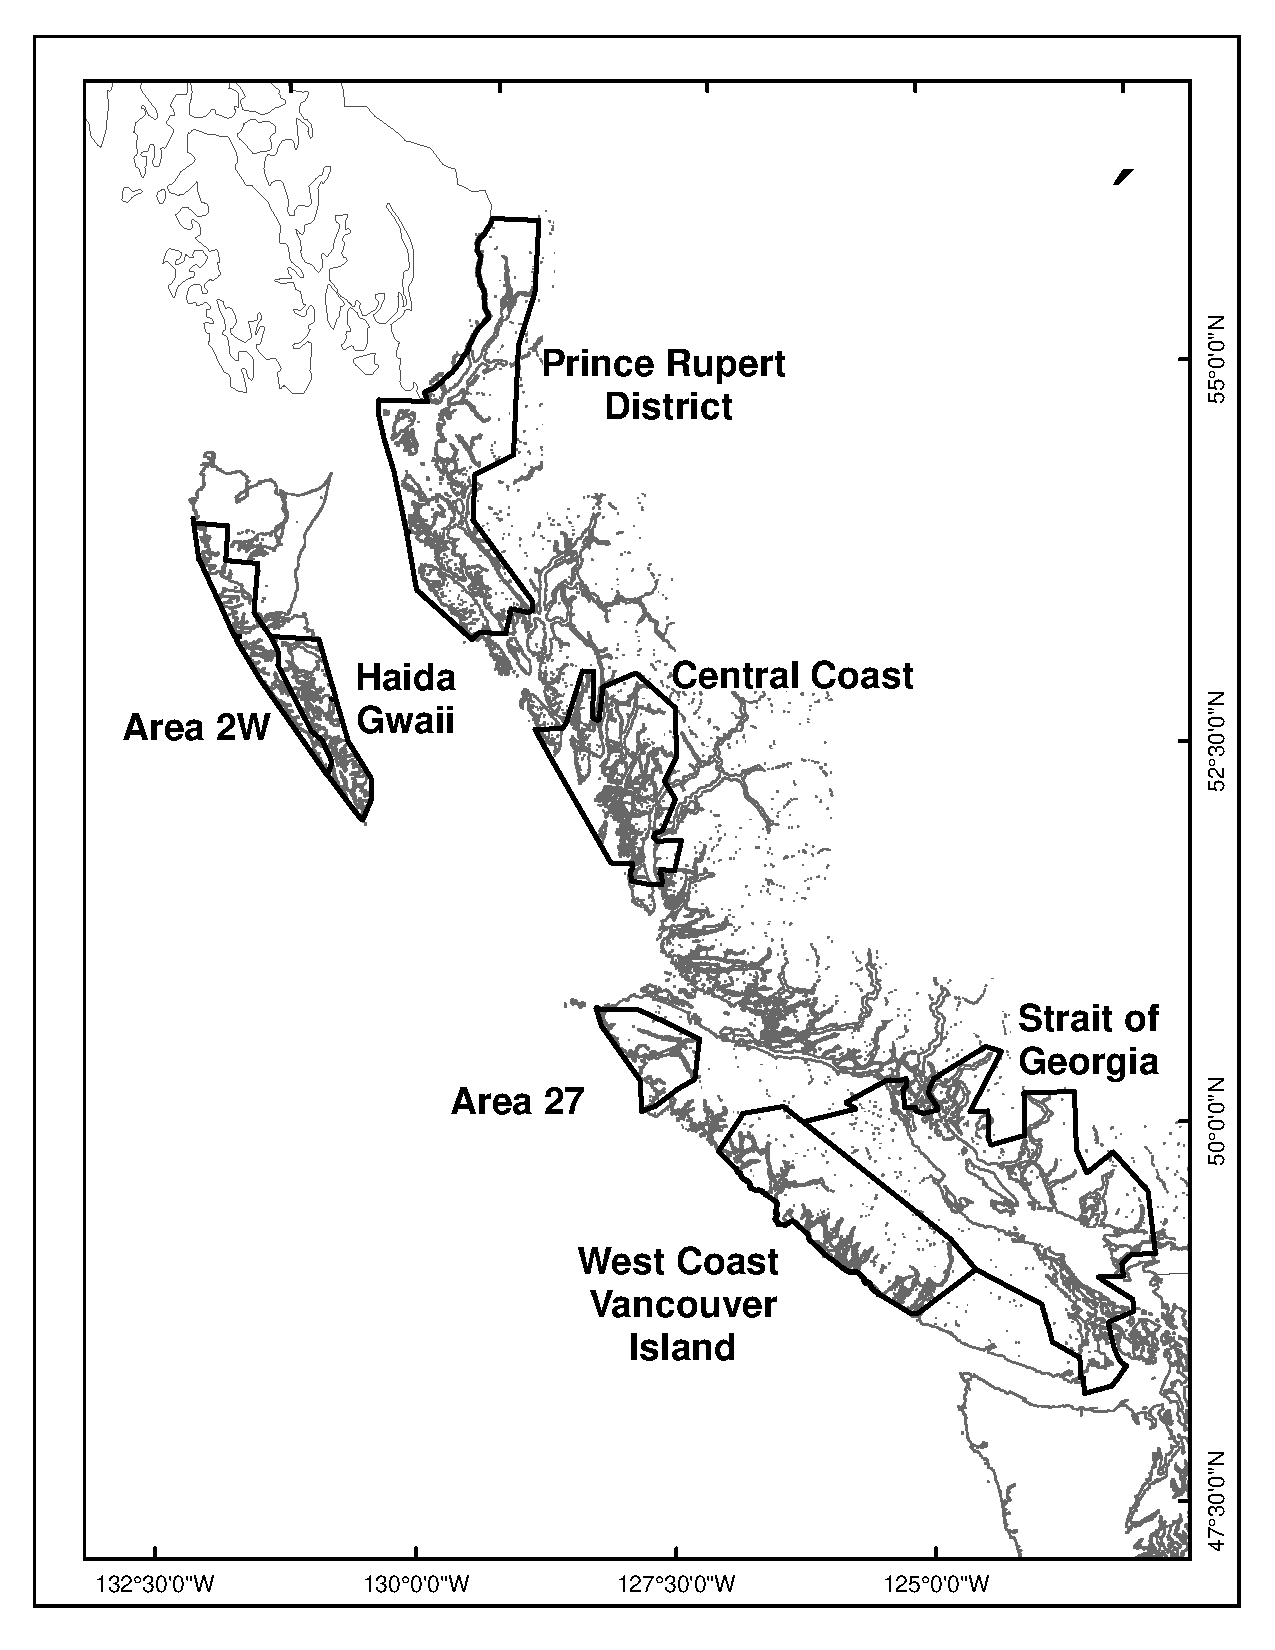
\includegraphics[width=\textwidth]{PBSfigs/Assessment_Regions_2W_27_2010_HG.pdf}
	\caption{B.C. herring major stock areas: Haida Gwaii (HG or QCI 2E), Prince Rupert District (PRD), Central
Coast (CC), Strait of Georgia (SOG), West Coast Vancouver Island (WCVI), and minor stock areas: Area 2W and
Area 27.}\label{Fig1}
\end{figure}
	
%%A reference for splines in selectivities can be found at \cite{aarts2009comprehensive}

%% SECTION Methods
%!TEX root = /Users/stevenmartell/Documents/CURRENT PROJECTS/iSCAM-trunk/fba/BC-herring-2011/WRITEUP/BCHerring2011.tex
\section{Methods}
	\subsection{Input data \& assumptions}
	\subsubsection{Catch data}
	For each of the statistical areas, the required input data for \iscam\ consists of a catch time series for each of the fishing fleets.  For the BC herring fishery, the annual total removals has been partitioned into three distinct fishing fleets (or fishing periods, see Figure \ref{FigCatch}).  The first fleet is a winter seine fishery that has been in operation since the start of the assessment in 1951, the second is a seine-roe fishery that commenced in 1972 in the Strait of Georgia, and the third fleet is a gillnet fishery that targets females on the spawning grounds. The model is fit to the catch time series information and assumes measurement errors are lognormal, independent and identically distributed.  The assumed standard deviation in the catch observations must be specified in the control file and it is assumed that measurement errors in the catch is the same for all fishing periods.  The units of the catch are given in 1000s of metric tons.
	
	In addition to the commercial catch, removals from fisheries independent surveys must also be specified in \iscam. Two additional fleets are specified to represent the spawn survey, where the spawn survey is broken into two distinct time periods pre-1988 and post-1988, the year when the survey switched from surface surveys to dive surveys.  This partitioning of the data is done for two reasons: (1) to allow for different catchability coefficients to be specified for the early and late periods, and to allow for more weight to be placed on the contemporary data due to improved precision in the estimates of egg layers. 

%TODO decide if the test fishery data is going to be looked at here or in the appendix
	In the case where the test fishery data has been separated from the seine roe fishery, an additional fleet is specified in the data file and fishing mortality rates for the test fishery are also estimated in years when the catch is greater than 0.
	
\begin{figure}[!tbp]
	% Requires \usepackage{graphicx}
	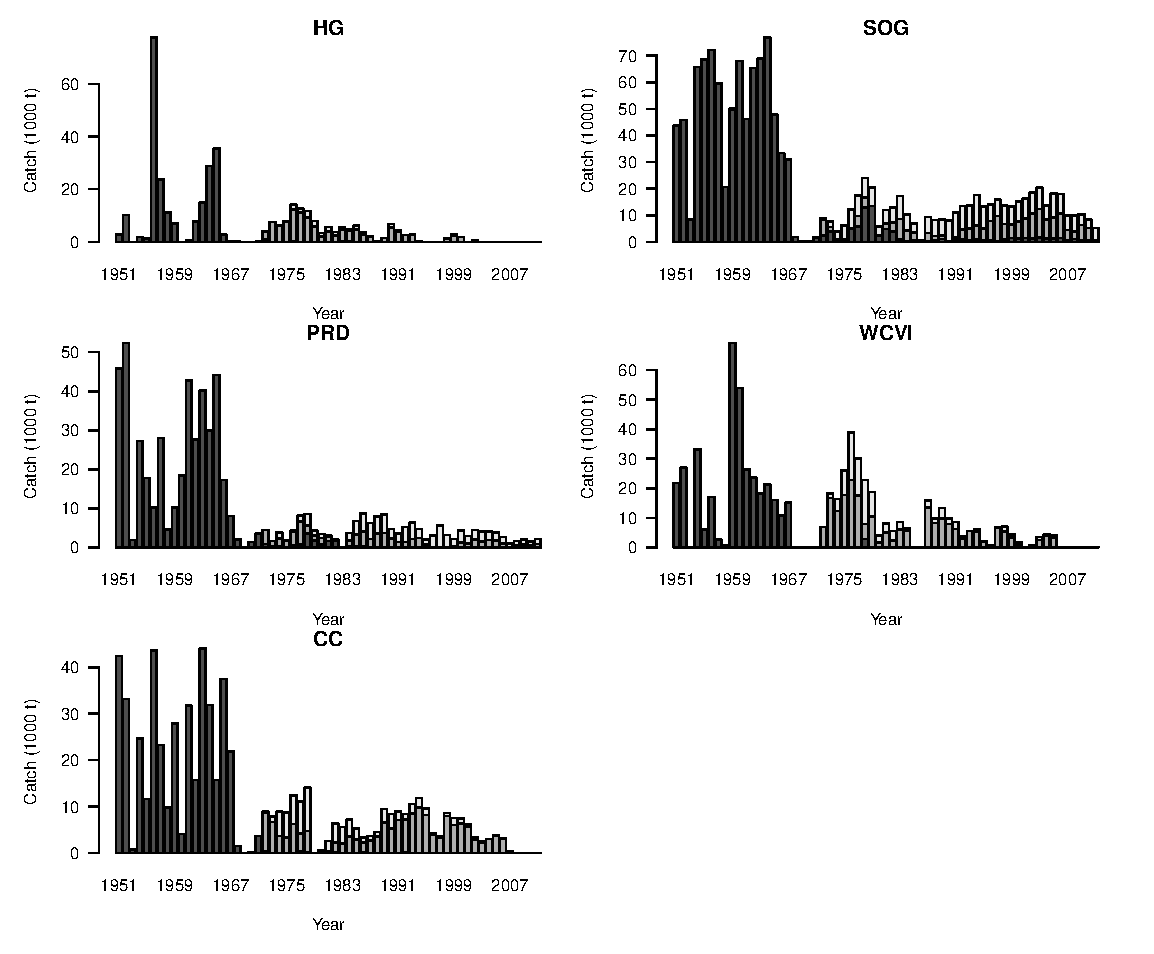
\includegraphics[width=\textwidth]{../Figs/iscam_fig_CatchMajorAreas.pdf}\\
	\caption{Historical catch of herring in the five major stock areas between 1951 and 2011 for the winter purse seine fishery (dark bars), seine-roe fishery (grey bars), and gillnet fishery (light grey bars). Units of catch are in thousands of metric tons.}\label{FigCatch}
\end{figure}
	
	\subsubsection{Relative abundance data}
Herring spawn surveys have been conducted throughout the B.C. coast beginning in the 1930s. Prior to 1988, spawn surveys were conducted from the surface either by walking the beach at low tide or using a drag from a skiff to estimate the shoreline length and width of spawn. Egg layers were sampled visually and are used to calculate egg densities following the methods of \cite{schweigert2001stock}. Beginning in 1988, herring spawn surveys using SCUBA methods were introduced and were implemented coastwide within a couple of years initially being conducted by DFO staff and eventually through contract divers hired through the test fishing program. Prior to the 2006 Larocque ruling, the test fishing program was funded through an allocation of fish by industry. In years since the 2006 Larocque ruling, the availability of resources to conduct dive surveys in all areas has been reduced. For 2011, dive surveys were conducted in all major and minor assessment regions, with the exception of Area 2W where snorkelling and surface survey methods were also used. As in earlier years, a few minor spawning beds outside the main assessment areas were surveyed by SCUBA or surface methods where resources permitted.


The locations of the spawning beds for the five major and two minor stock areas are shown in Figure \ref{figSpawnMaps}.  Egg density estimates are used to calculate a fishery-independent index of herring spawning biomass, referred to as the spawn survey index hereafter \citep{schweigert2001stock}.

\begin{figure}[!tbp]
	% Requires \usepackage{graphicx}
	\centering
	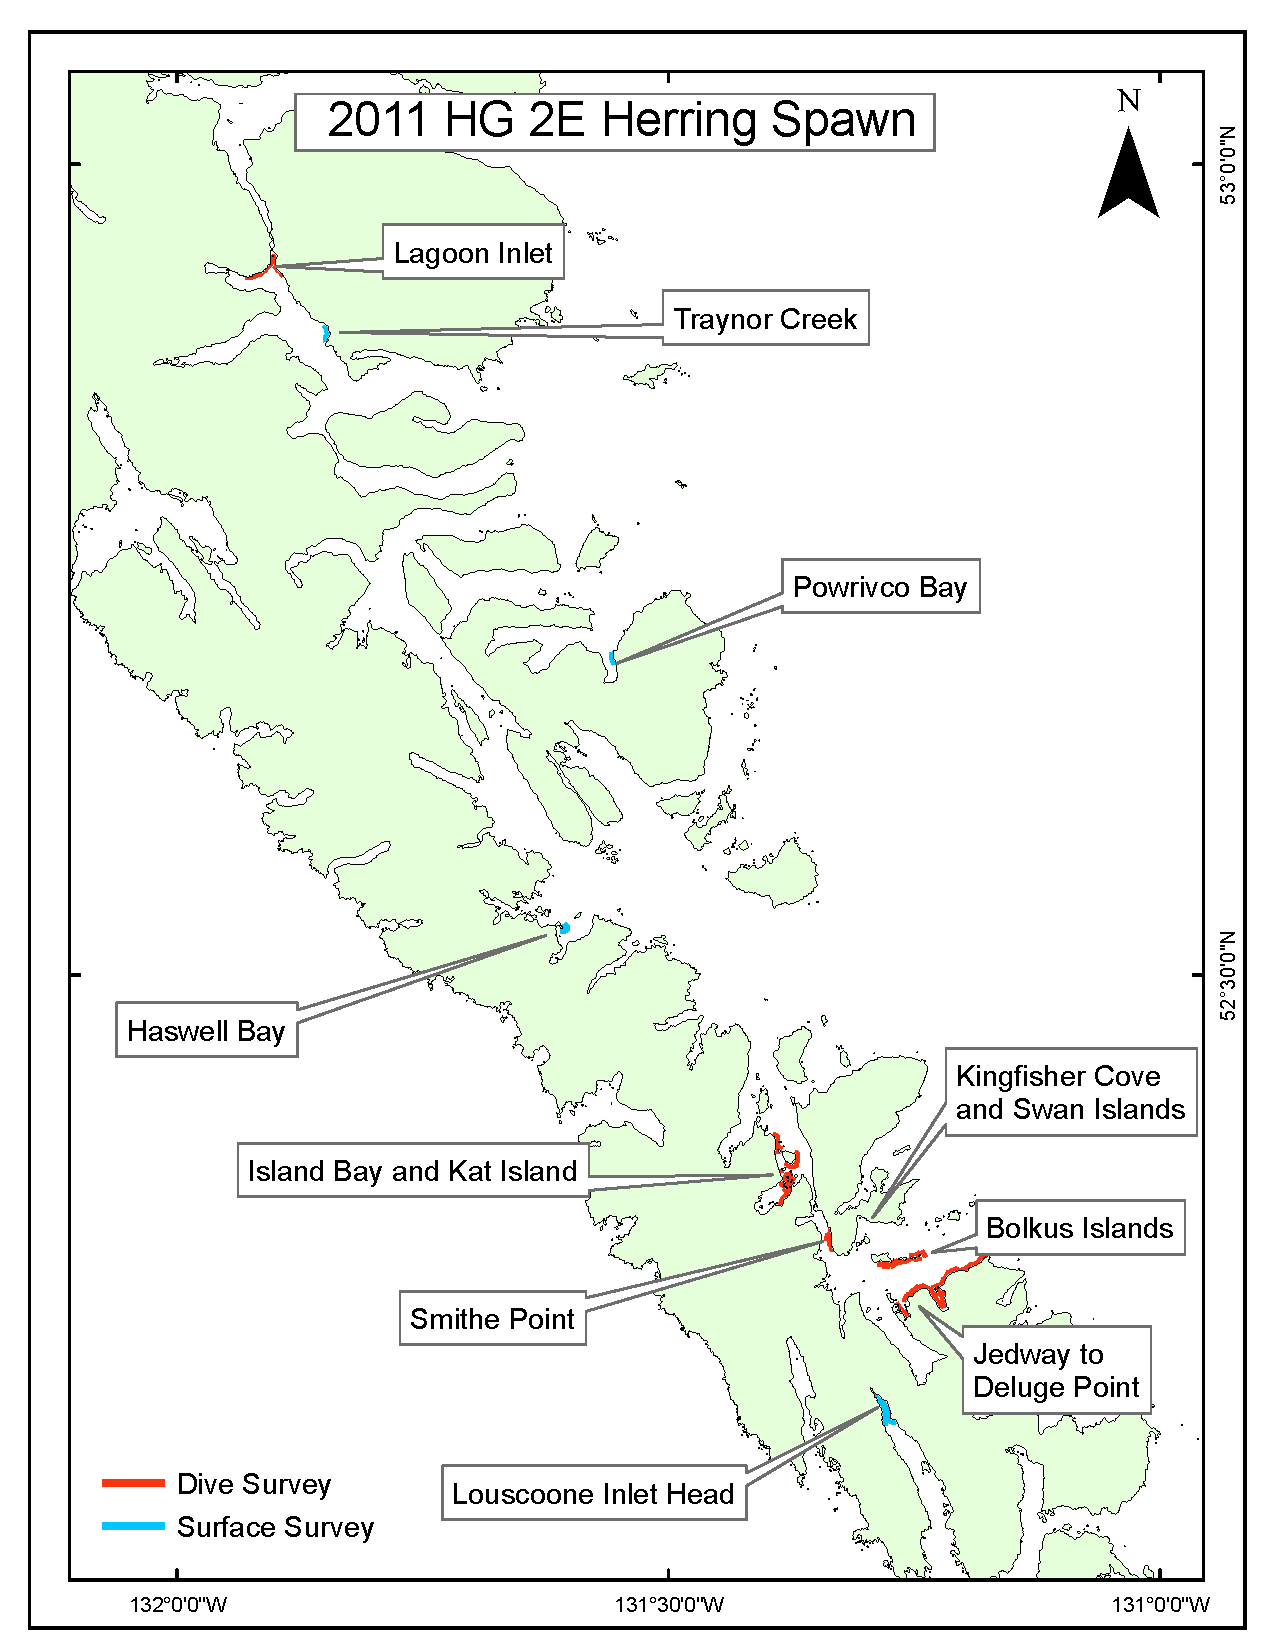
\includegraphics[scale=0.35]{../Figs/PBSfigs/2011_spawn_HG_2E_July13.pdf}
	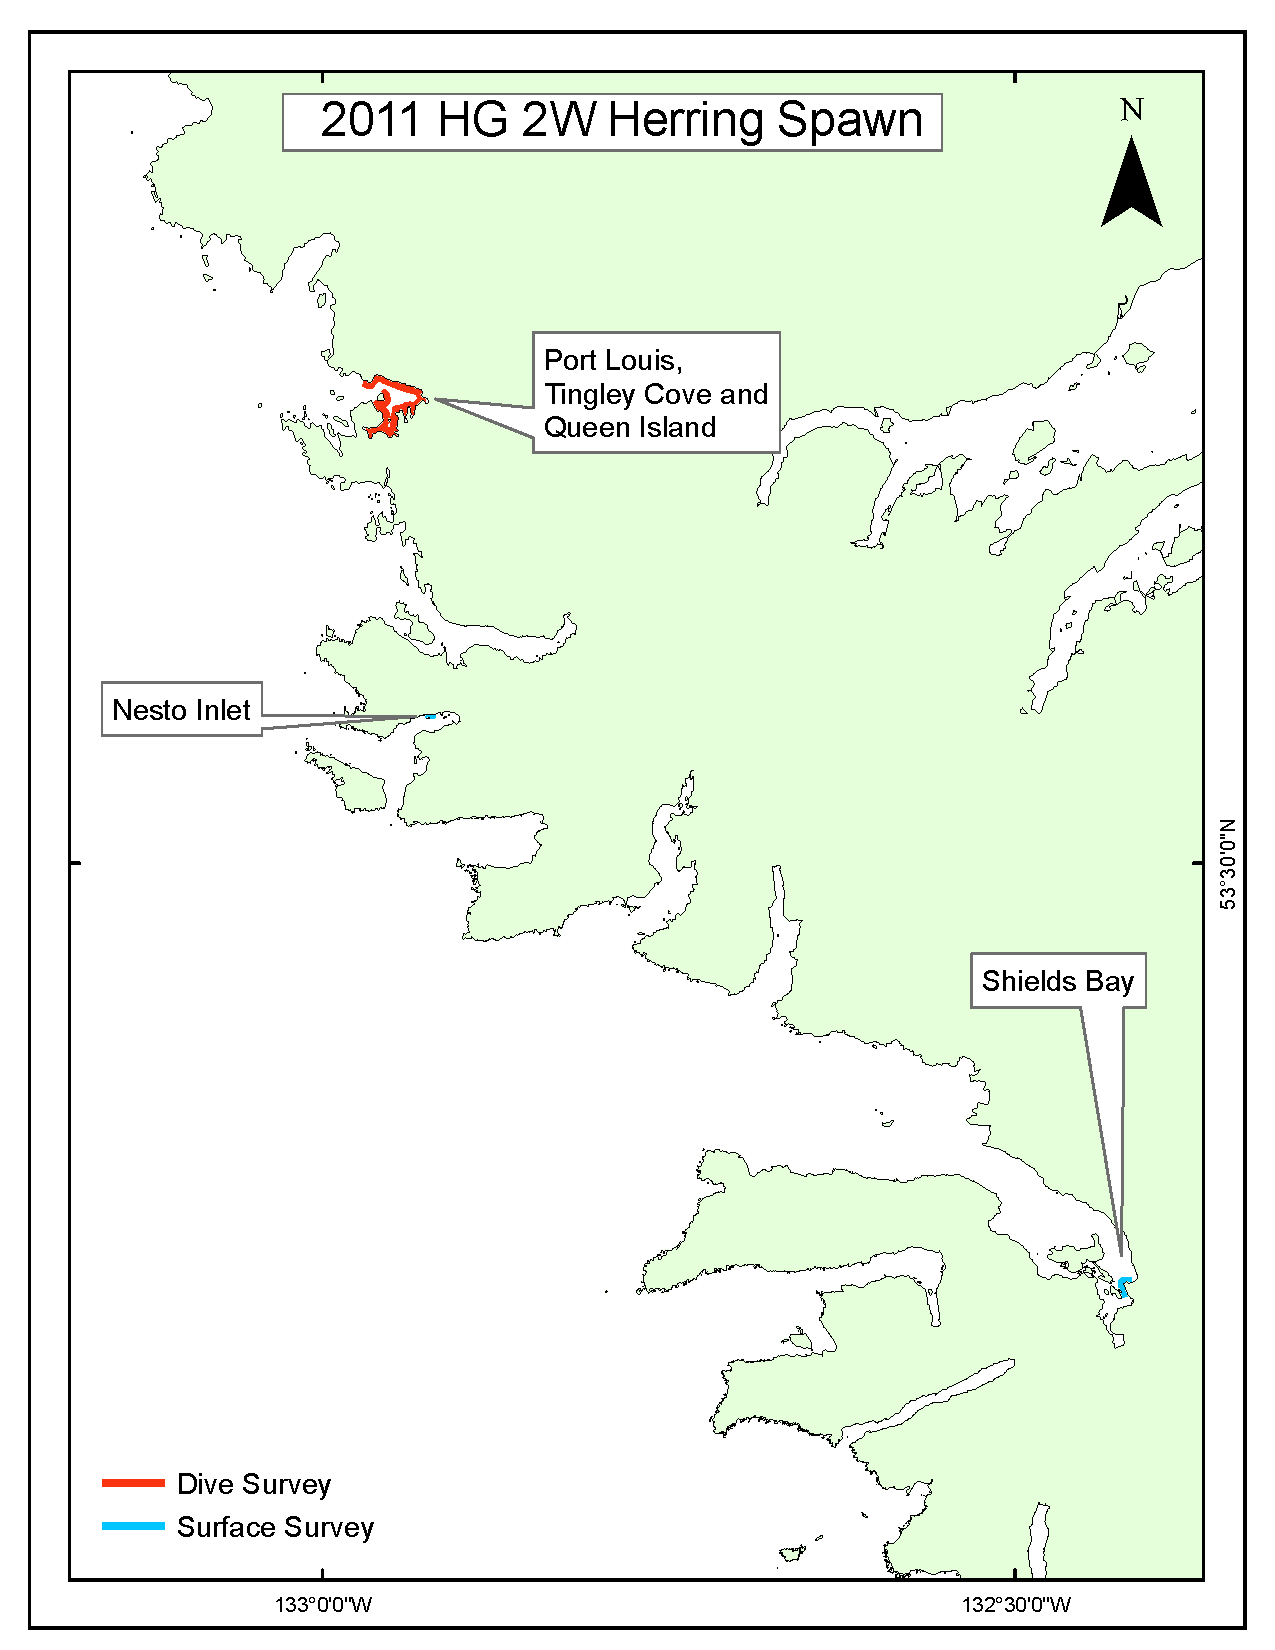
\includegraphics[scale=0.35]{../Figs/PBSfigs/2011_spawn_HG_2W_July13.pdf}\\
	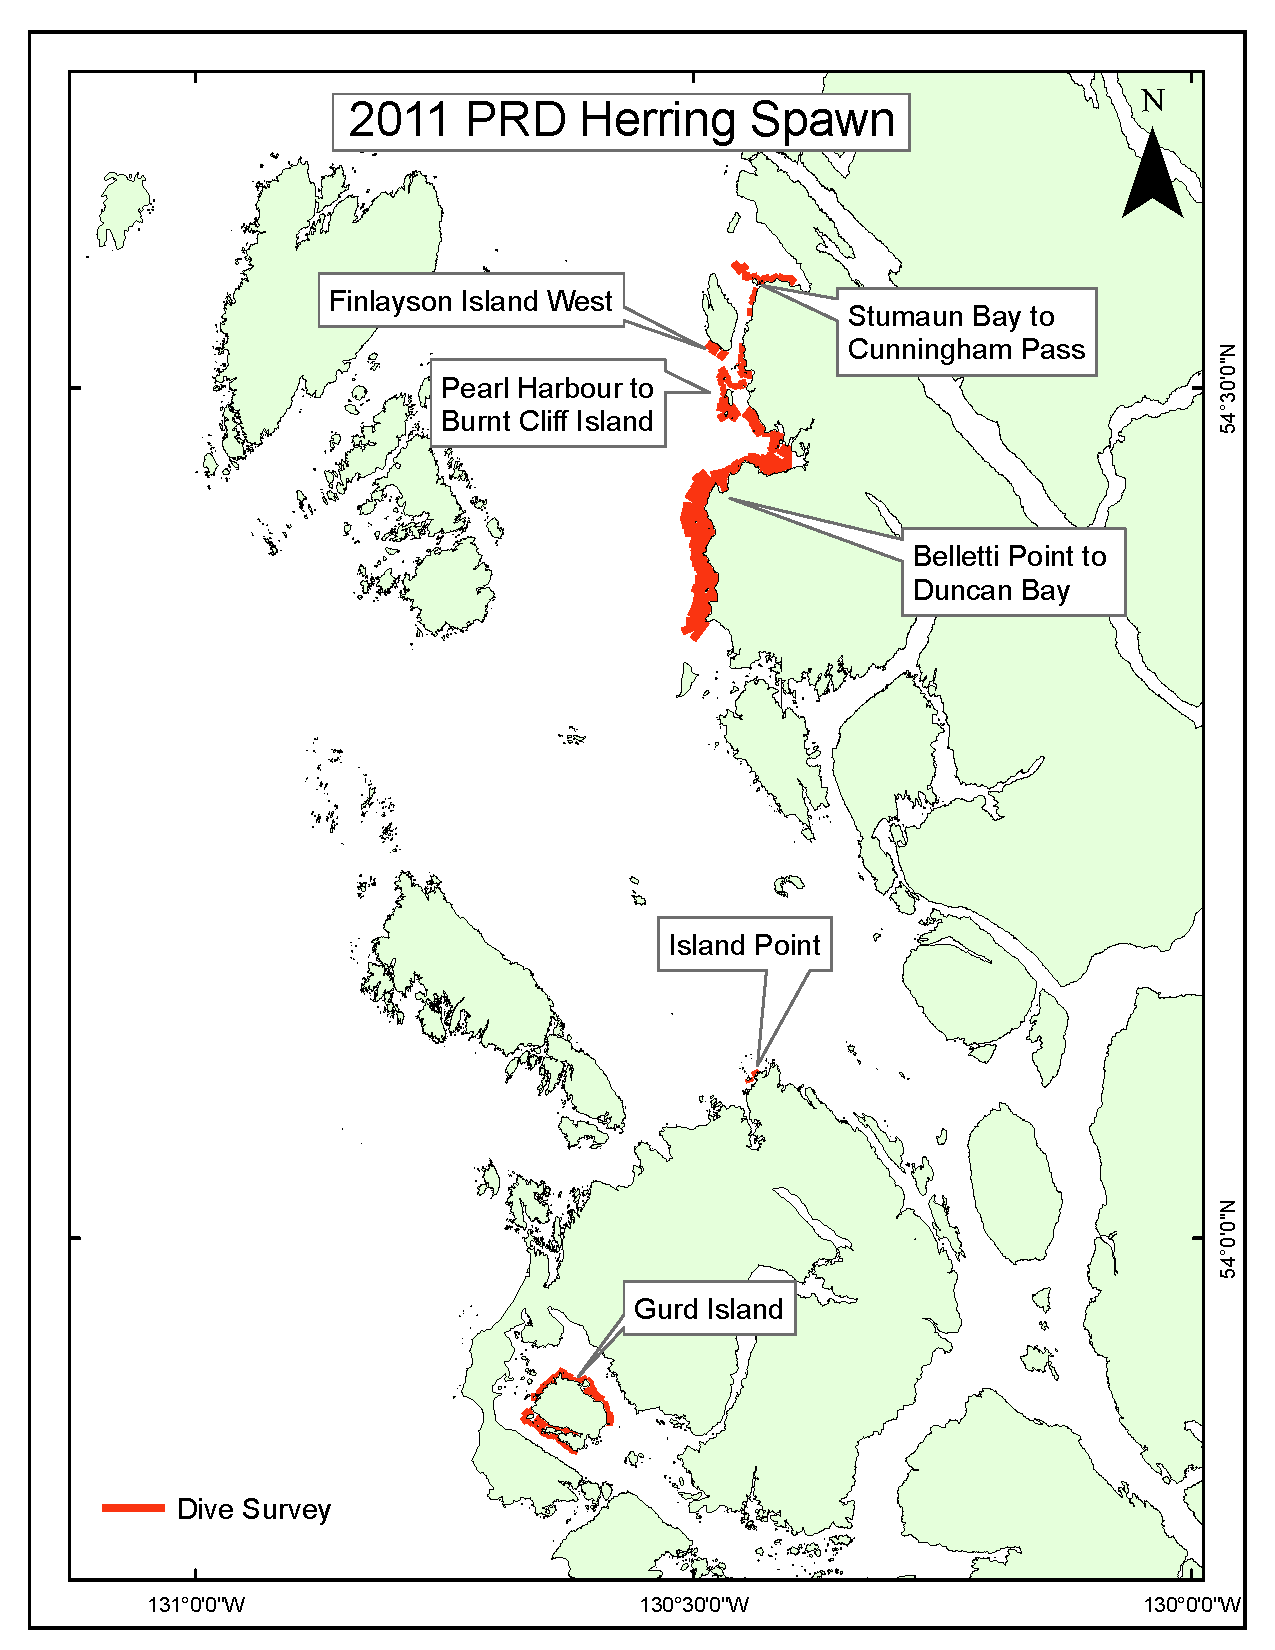
\includegraphics[scale=0.35]{../Figs/PBSfigs/2011_spawn_PRD_July13.pdf}
	\caption{Preliminary Spawning activity for Haida Gwaii (top panels) and Prince Rupert District (bottom) in 2011.}
\end{figure}
\begin{figure}[!tbp]
	% Requires \usepackage{graphicx}
	\ContinuedFloat
	\centering
	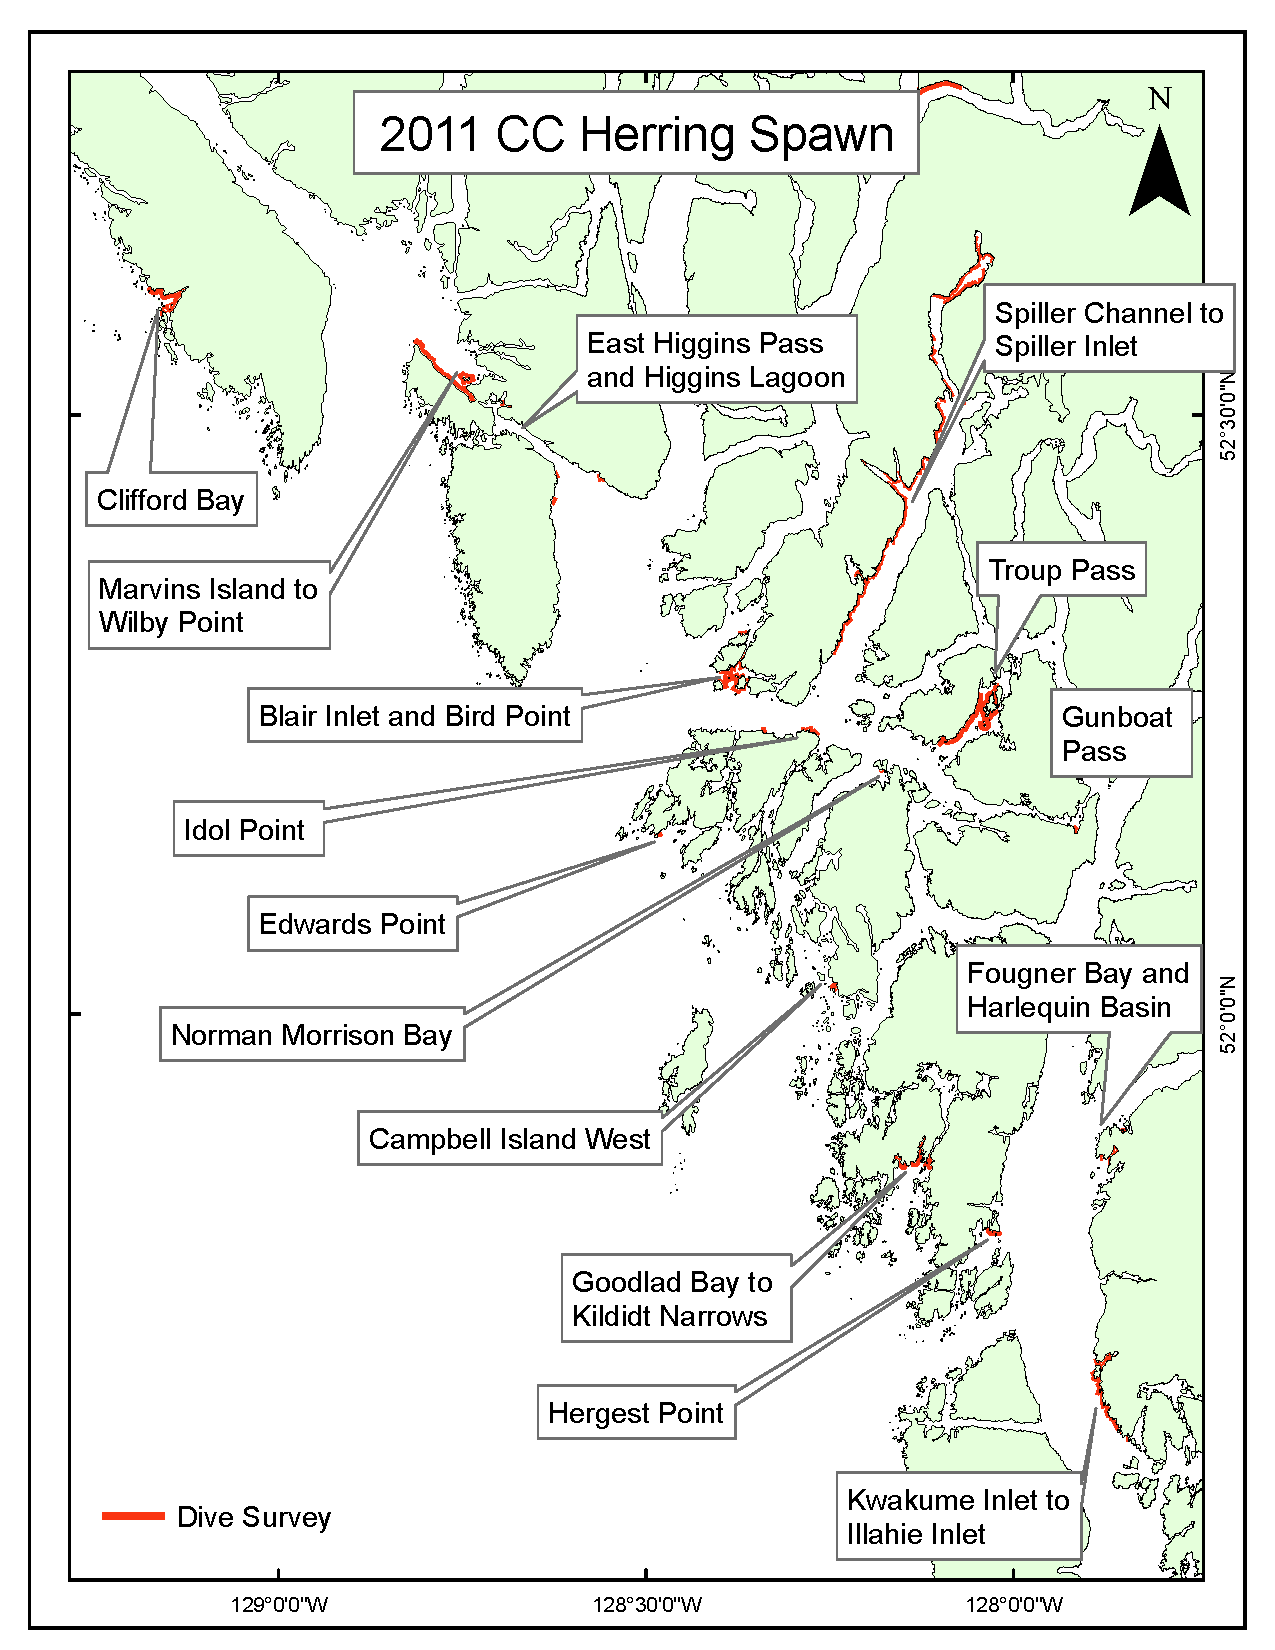
\includegraphics[scale=0.35]{../Figs/PBSfigs/2011_spawn_CCJuly13.pdf}
	%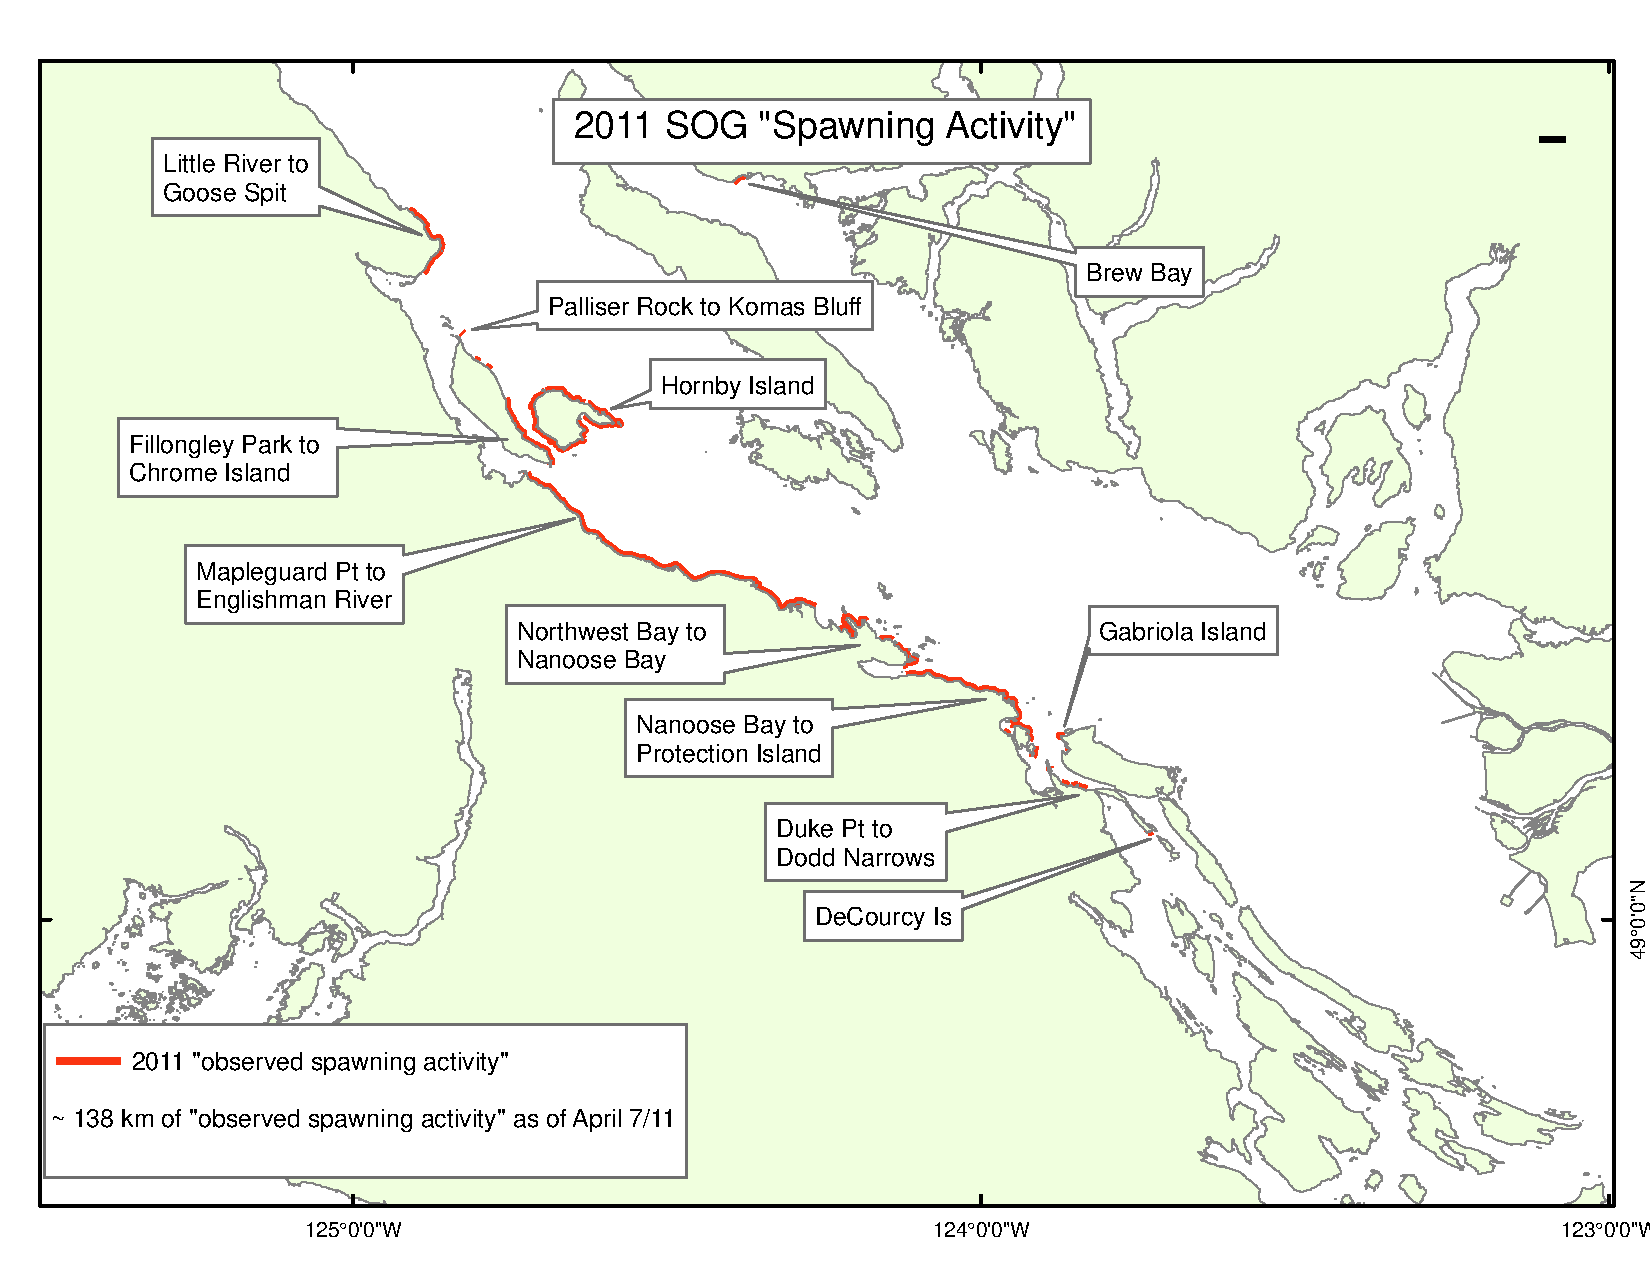
\includegraphics[scale=0.5]{../Figs/PBSfigs/2011-SOG-Prelim-WG.pdf}
	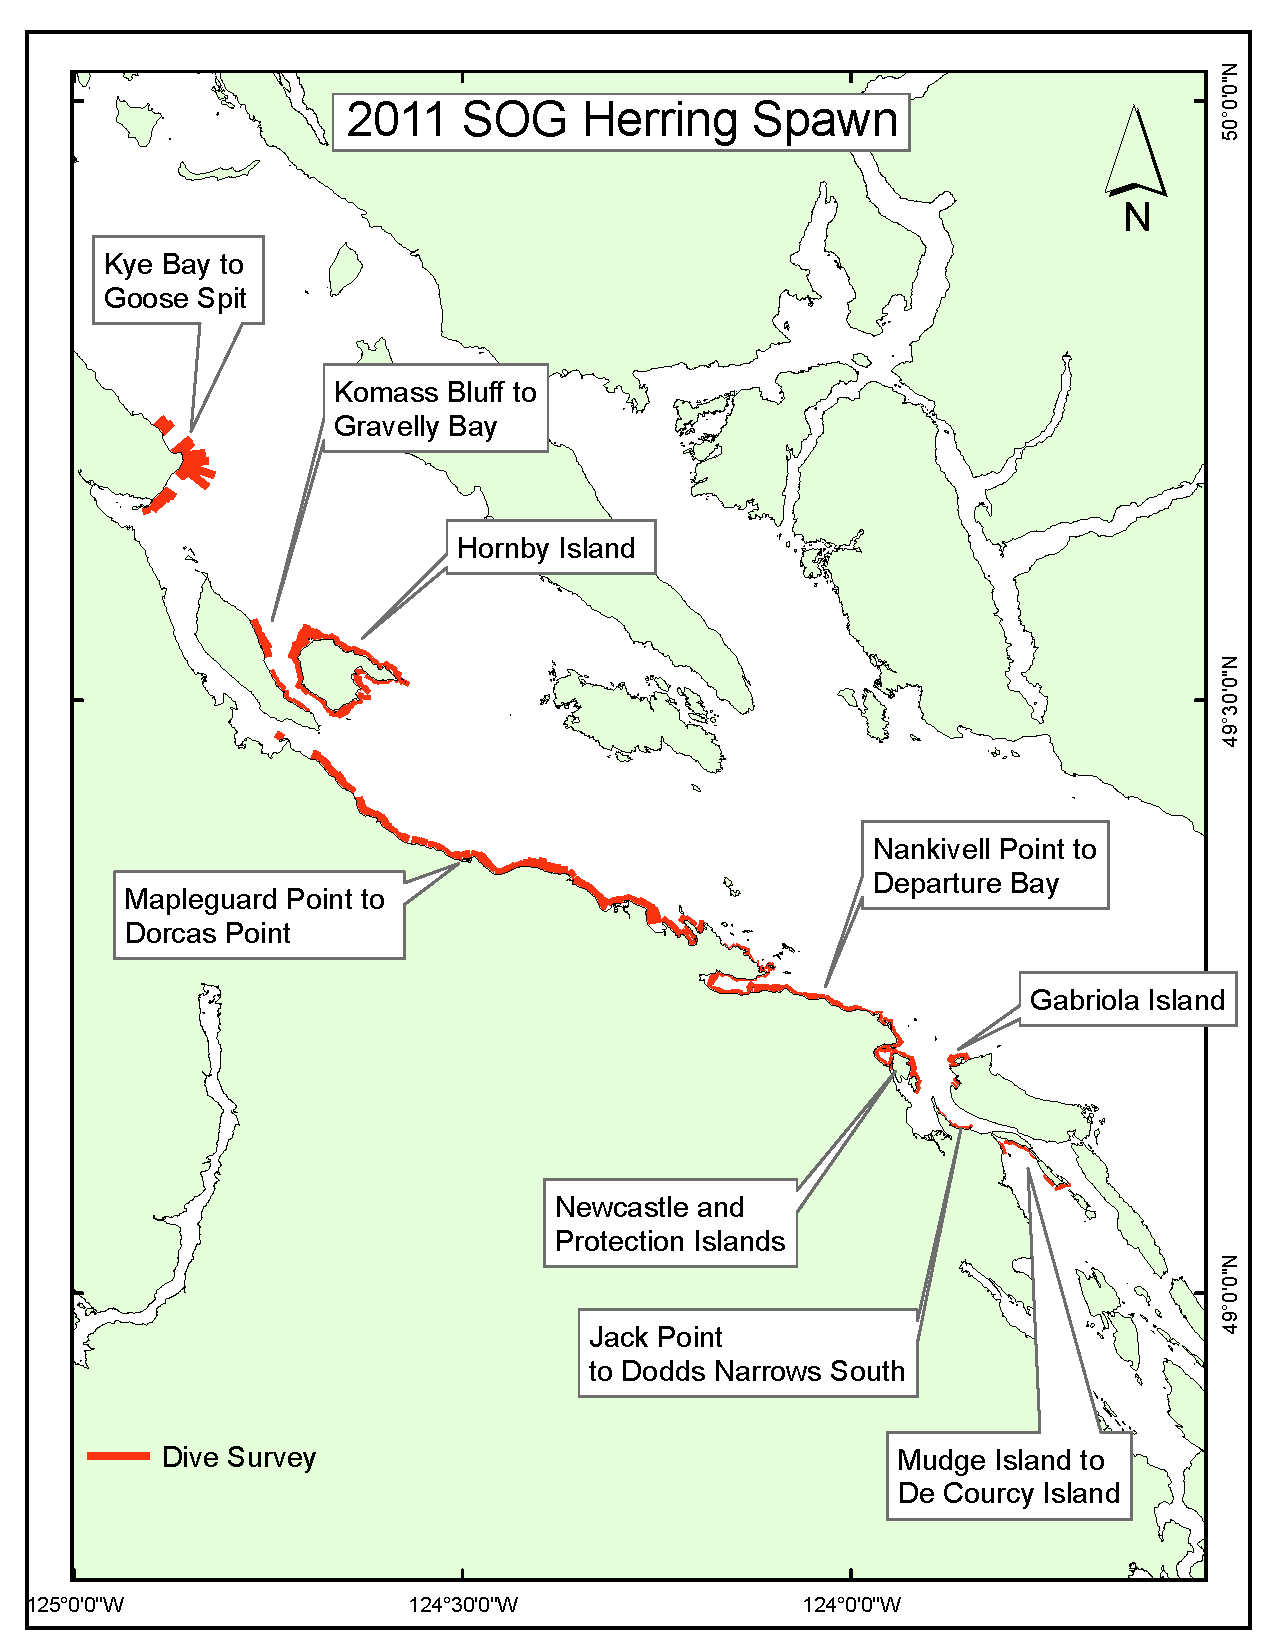
\includegraphics[scale=0.35]{../Figs/PBSfigs/2011_spawn_SOG_July13.pdf}\\
	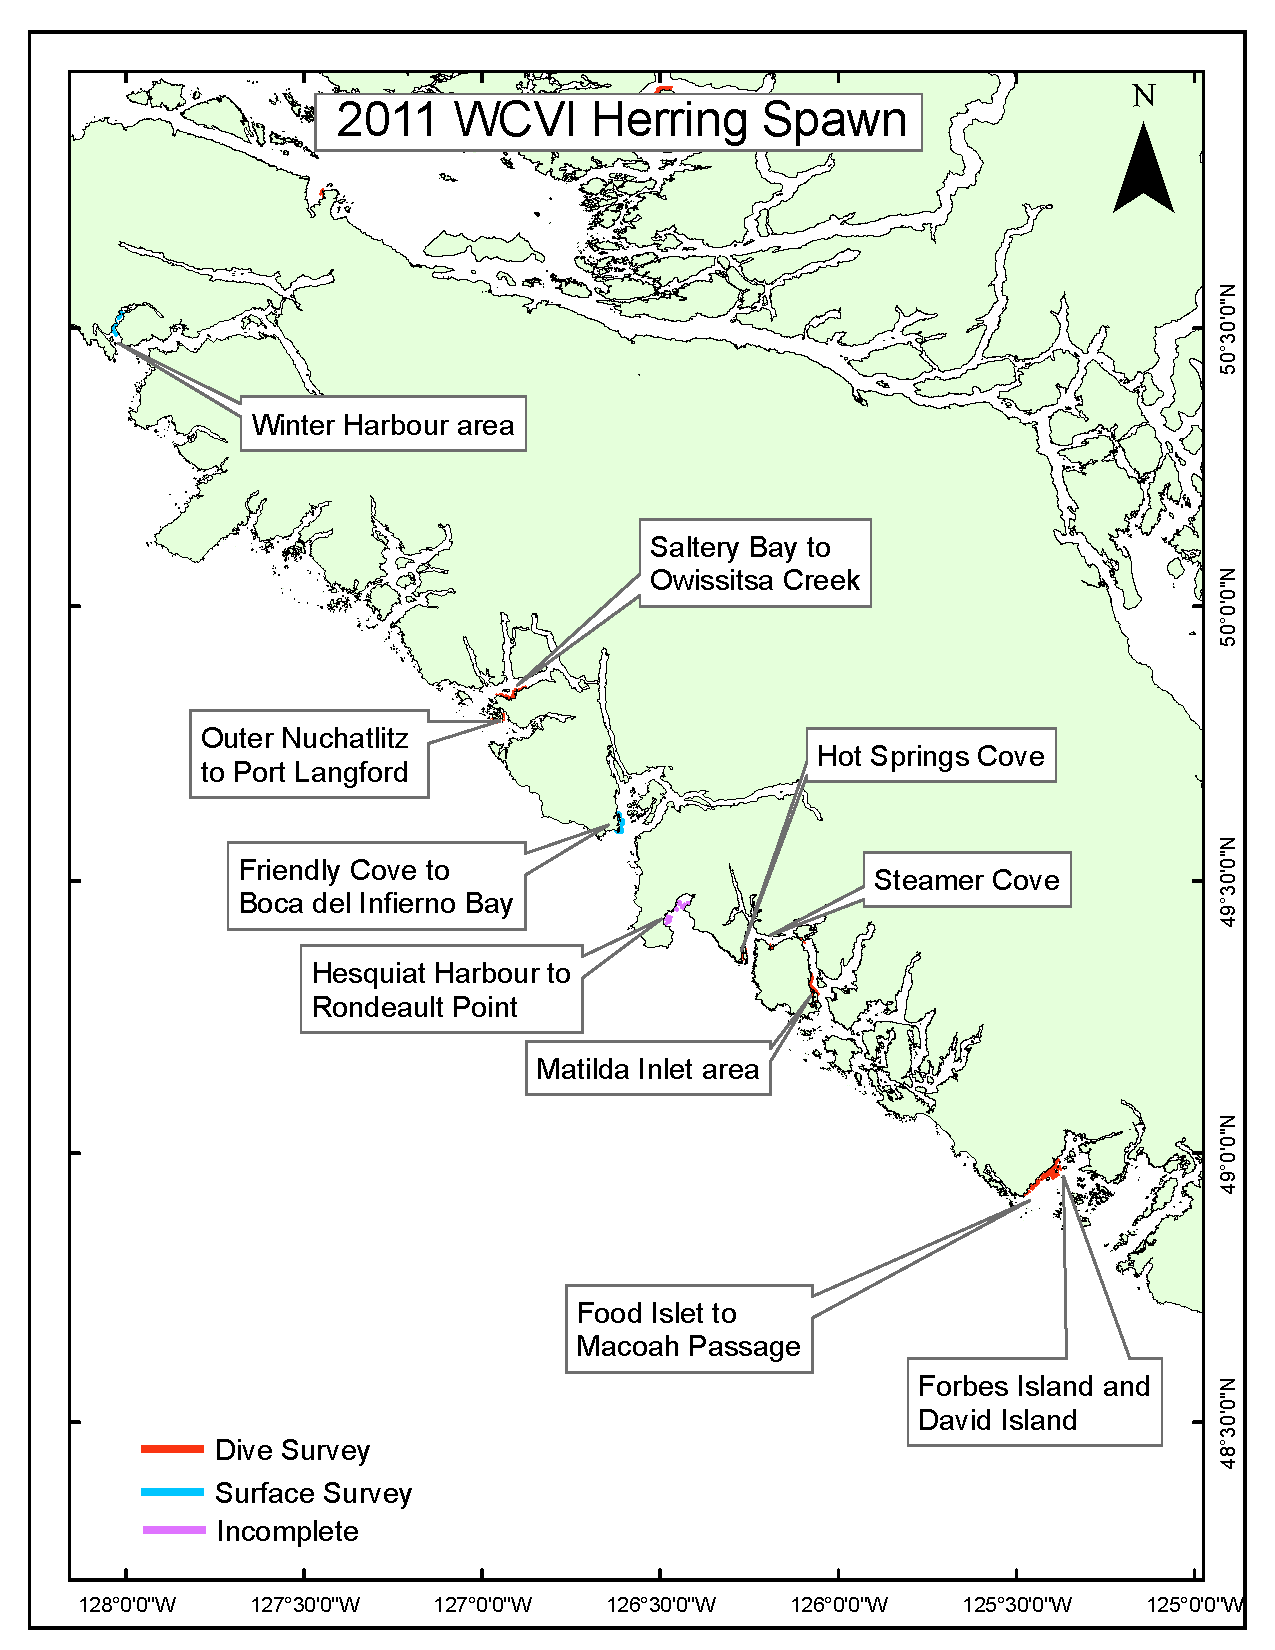
\includegraphics[scale=0.35]{../Figs/PBSfigs/2011_spawn_WCVI_August16.pdf}
	\caption{Preliminary Spawning activity for Central Coast (top left panel), Strait of Georgia (top right) in 2011 and west coast Vancouver Island (bottom).}\label{figSpawnMaps}
\end{figure}
% \begin{figure}[!tbp]
% 	% Requires \usepackage{graphicx}
% 	\ContinuedFloat
% 	\centering
% 	%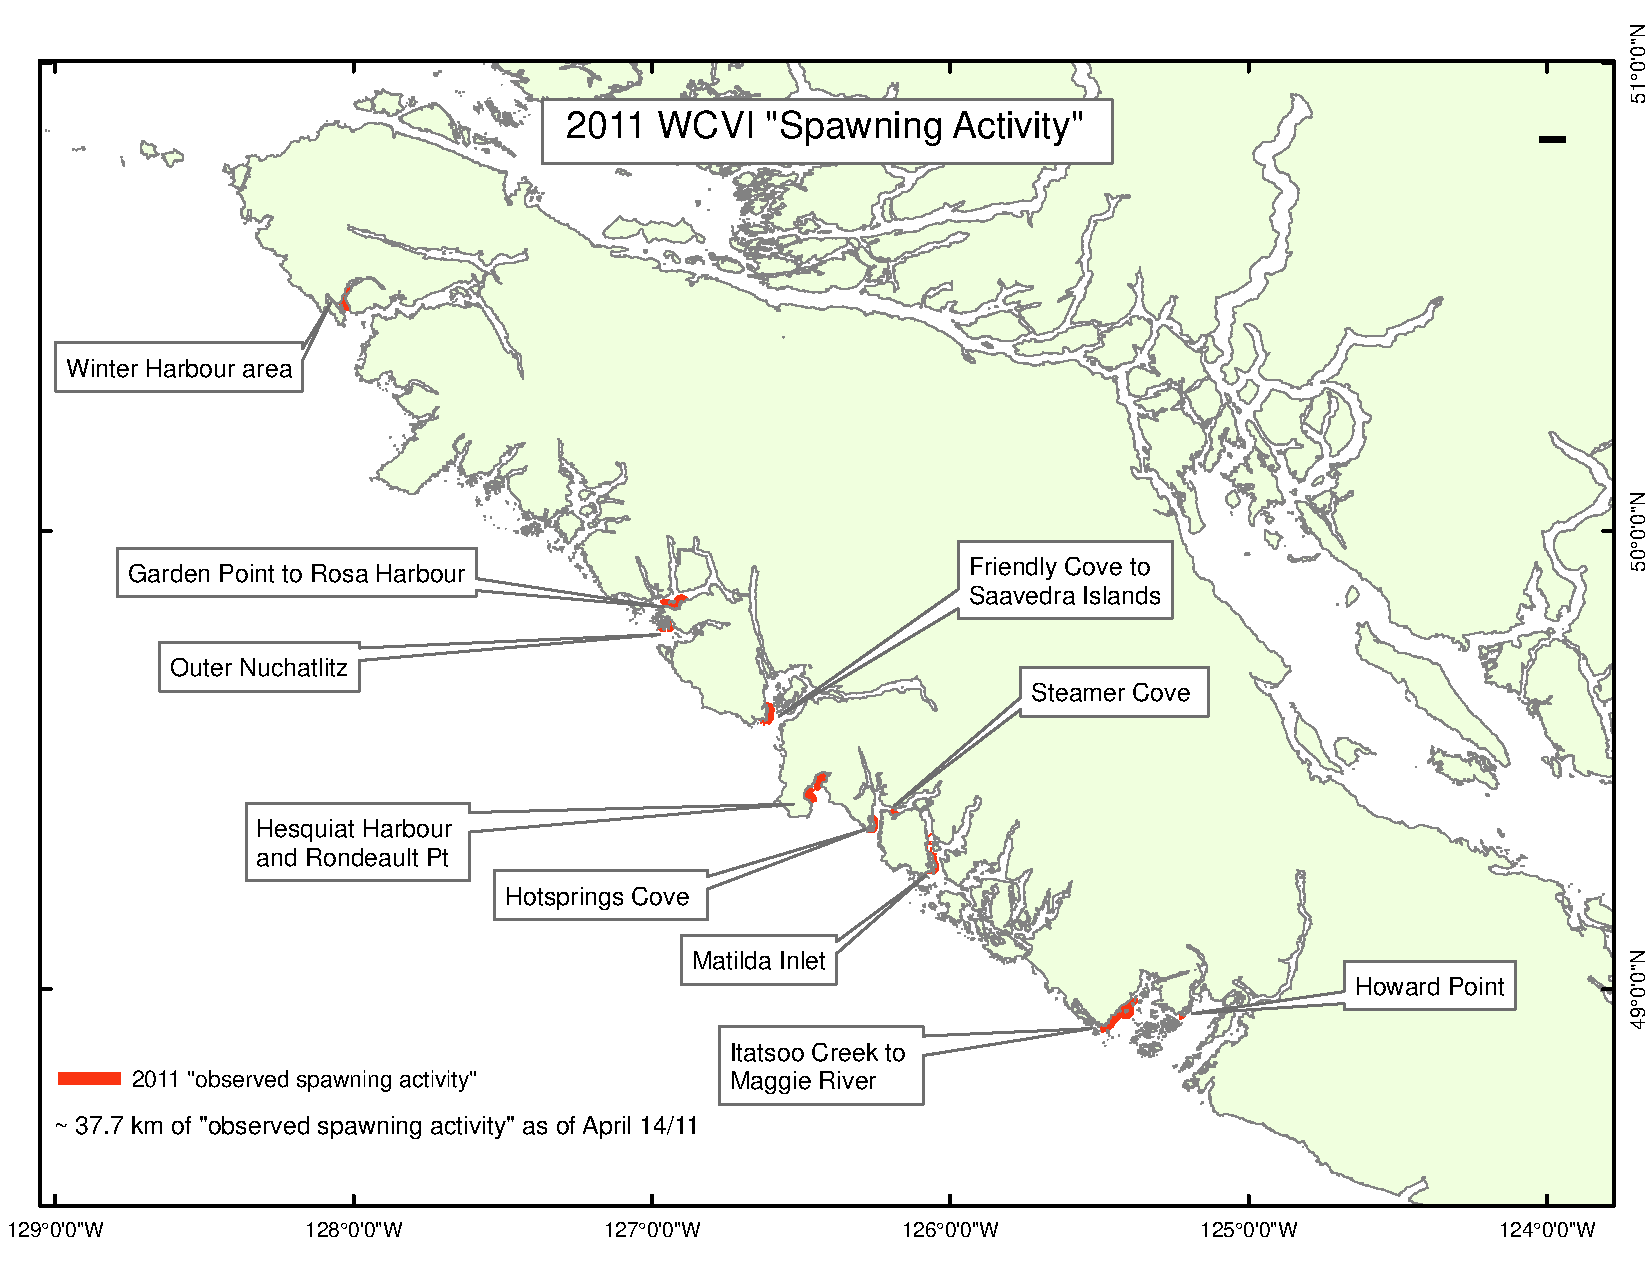
\includegraphics[scale=0.5]{../Figs/PBSfigs/2011-WCVI-Prelim-WG.pdf}\\
% 	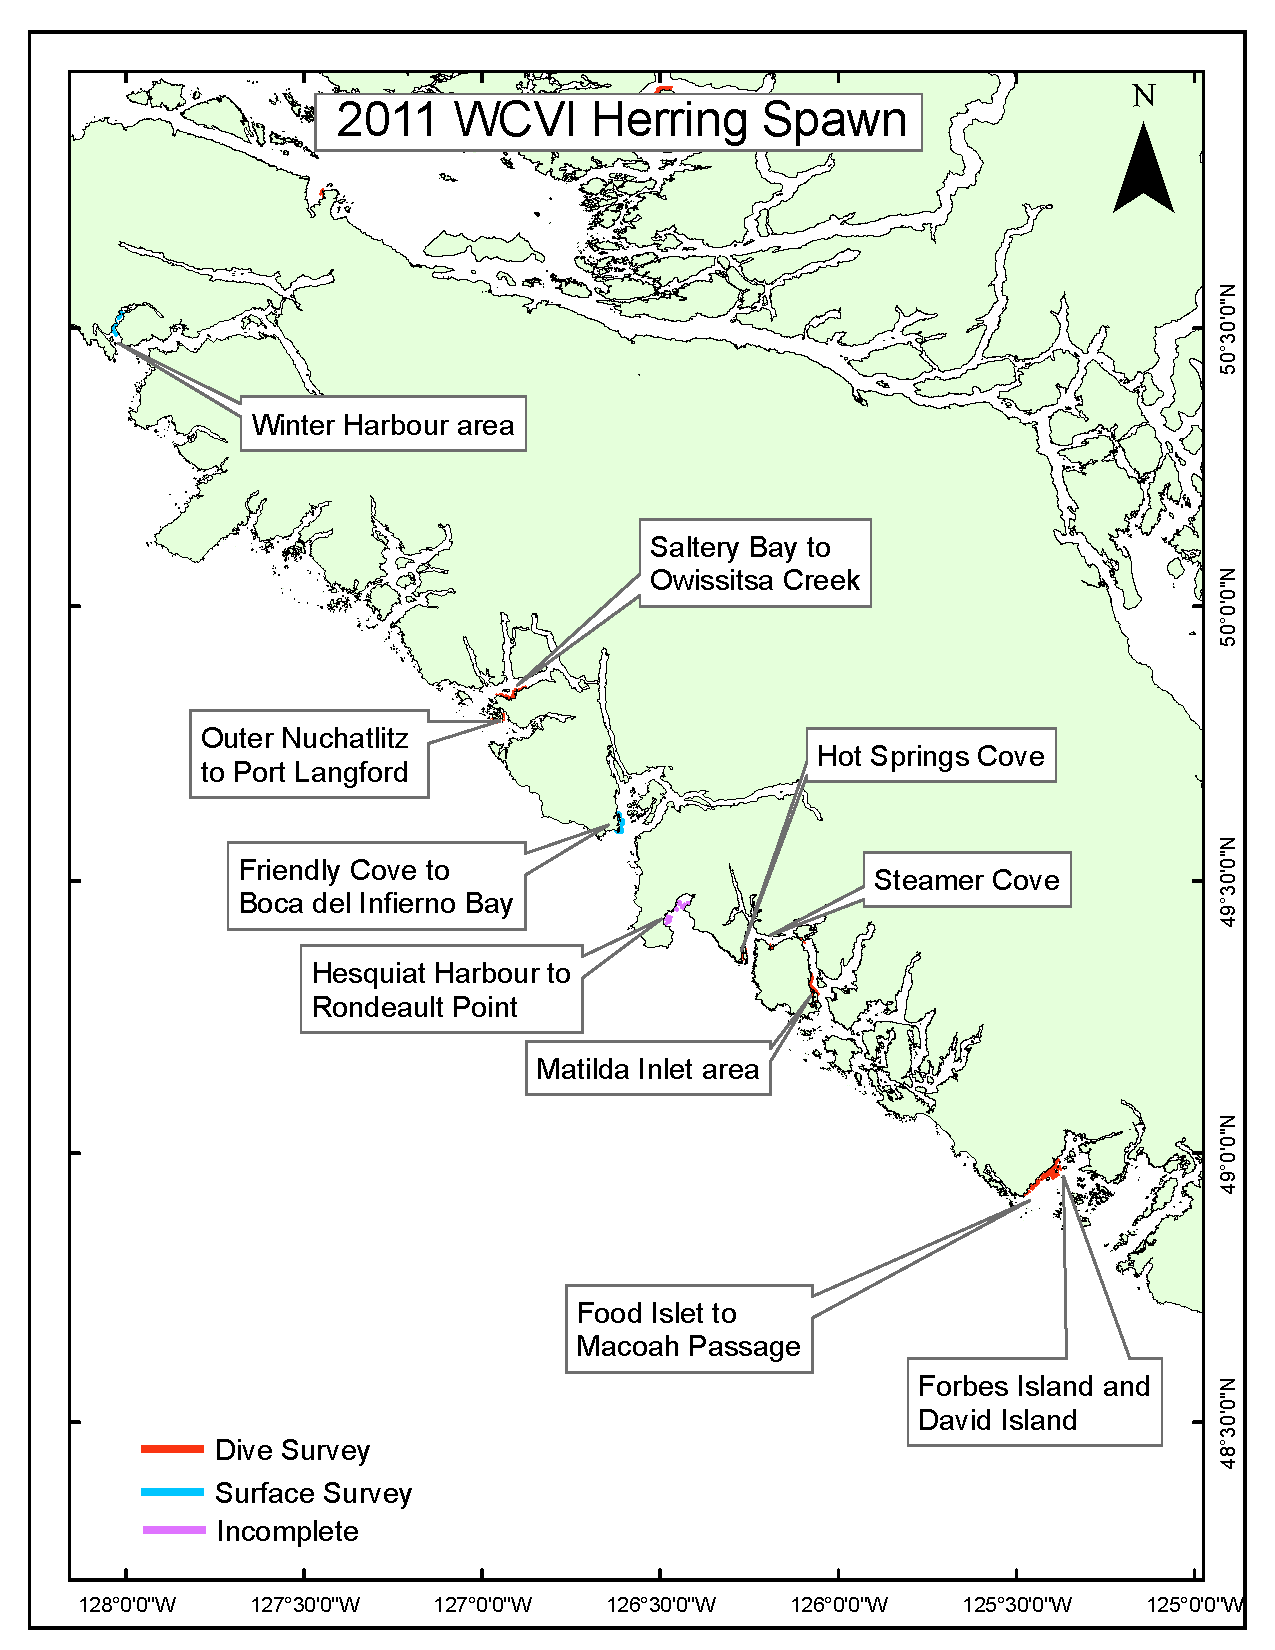
\includegraphics[scale=0.5]{../Figs/PBSfigs/2011_spawn_WCVI_August16.pdf}\\
% 	\caption{Preliminary Spawning activity in 2011 for the West Coast of Vancouver Island (includes minor stock area 27).}\label{figSpawnMaps}
% \end{figure}

	The spawn survey is conducted after the fisheries in the area have been completed; therefore, it is assumed that all the mortality for the year has occurred just prior to commencing the spawning survey. The fisheries independent survey estimates egg density and total spawn area, and from this information the total female spawning biomass can be estimated assuming the 200 eggs per gram of female  or 100 eggs per gram of mature  individuals \citep{hay1985reproductive,hardwick1973biomass}. The assumed selectivity for the spawn survey is fixed to the maturity schedule for herring.  	
	
\begin{figure}[!tbp]
	% Requires \usepackage{graphicx}
	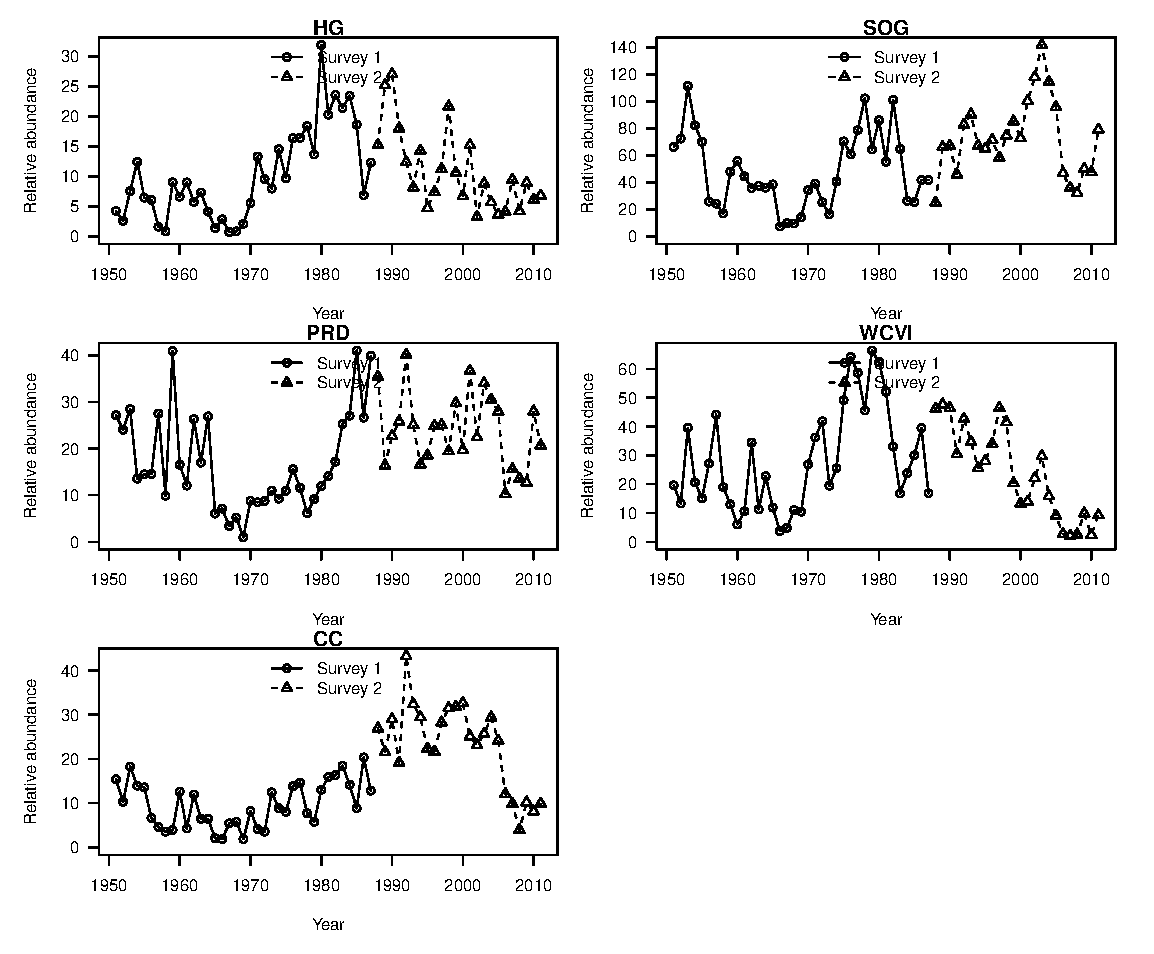
\includegraphics[width=\textwidth]{../Figs/iscam_fig_SurveyMajorAreas.pdf}\\
	\caption{Spawn survey index for Strait of Georgia between 1951 and 2011. The units are actual estimates of spawning biomass (1000s tons), but only the trend information is used in the model fitting.}\label{FigSurvey}
\end{figure}
	
	\subsubsection{Biological samples}
	
	Biological samples are collected from both commercial catch and from the test fishery program.  Commencing  in 1975, test fishery charters supplemented biological samples in areas with poor sampling that was not representative of the stock in that area (i.e., fishing solely on spawning aggregations), or in closed areas. Prior to 2006, test fishing charters were funded through an allocation of fish to the test program; the program is now fully funded by DFO.  Through a contract with DFO, the Herring Conservation and Research Society (HCRS) sub-contracts a number of vessels to collect biological samples.  Industry also conducts pre-season test sets for roe-quality testing in open areas and supplementary biological samples are provided as part of this program.  The following data are collected for all biological samples: fish length, weight, sex, and maturity.  Subsequently these sources of data are combined and information on weight-at-age and proportion-at-age become input data for the stock assessment model.
	
	During the 2010/2011 season a total of 248 biological samples were collected, of which 151 were collected from the test fishery, 57 were collected from the roe fishery, 16 from the food \& bait fishery, 4 from Spawn on Kelp (SOK) operations, and 16 from the summer trawl research survey (Table \ref{table:PartII:bioSamples}).  Note that the definition of a sample is roughly 100 individual fish.  A summary of biological samples collected from commercial and pre-fishery charters from 2002/03--2010/11 is presented in Table \ref{table:PartII:sampleSizes}).

\begin{table}
	\caption{Summary of biological samples collected and processed from all sources from the 2010/11 herring season.}
	\label{table:PartII:bioSamples}
	\begin{center}
		\begin{tabular}{cccccc}
		\hline
		& \multicolumn{3}{c}{Commercial samples} &  \\
		Stock & Roe fishery & SOK fishery & F\&B & Test fishery & Research\\
		\hline
		HG (QCI 2E) &  &  &  & 13\\
		PRD & 29 & 1 &  & 24\\
		CC &  &  &  & 30\\
		SOG & 18 &  & 20 & 60\\
		WCVI &  &  &  & 14 & 16\\
		Area 2W &  &  &  & 10\\
		Area 27 &  & 3\\
		Other Areas\\
		\hline
		Total & 57 & 4 & 16 & 151 & 16\\
		\hline
		\end{tabular}
	\end{center}
\end{table}

\begin{table}
	\caption{Summary of biological samples collected and processed from commercial catch and test fishery charters from 2002/03-2010/11.}
	\label{table:PartII:sampleSizes}
	\begin{center}
\begin{tabular}{cccc}
\hline
Fishing season & Commercial fishery samples & Charter and research samples & Total\\
\hline
2002/03 & 120 & 287 & 407\\
2003/04 & 79 & 222 & 301\\
2004/052 & 83 & 191 & 274\\
2005/06 & 46 & 164 & 210\\
2006/07 & 114 & 85 & 199\\
2007/08 & 116 & 103 & 219\\
2008/09 & 87 & 136 & 223\\
2009/10 & 78 & 135 & 213\\
2010/11 & 81 & 167 & 248\\
\hline
\end{tabular}
	
	\end{center}
\end{table}
	
	
	
	%%Insert Summary of biological samples from the 2010/2011 season here:
	
	%%Insert Summary of biological samples collected and processeed from commercial catch etc. here (Table 2 from Cleary 2011).
	
	\subsubsection{Age composition data}
	
	Ageing data, through the reading of fish scales, are collected from the biological samples taken from the commercial fisheries and test fishery charters. Age composition data is used to determine proportions-at-age and is an essential source of input data to the herring stock assessment model.
	
	Catch-at-age data from the winter seine fishery (top panels of Figures \ref{FigAgeCompsHG}-\ref{FigAgeCompsWCVI}) tend to consist of younger fish in comparison to the age composition data from the seine-roe and gillnet fleets post 1970. The shaded polygons in Figures \ref{FigAgeCompsHG}-\ref{FigAgeCompsWCVI} approximates the 95\% distribution of ages in the catch.  Roughly 90\% of the fish landed in the winter seine fishery were younger than age-7, and younger than age-6 in recent years.  In both the winter seine and seine-roe fishery age-2 fish are frequently landed; whereas, age-2 fish are rarely landed in the gillnet fishery, and fish do not appear to fully recruit to the gear until at least 4-5 years of age.  The mean age of the catch appears to be increasing between 2008 and 2010 in both the gillnet and winter seine fishery, and there is no obvious trend in the seine roe fishery.  There is however a declining trend in the older ages caught in the seine-roe fishery since 2006 (erosion of age-structure).

\begin{sidewaysfigure}[!tbp]
	% Requires \usepackage{graphicx}
	\centering
	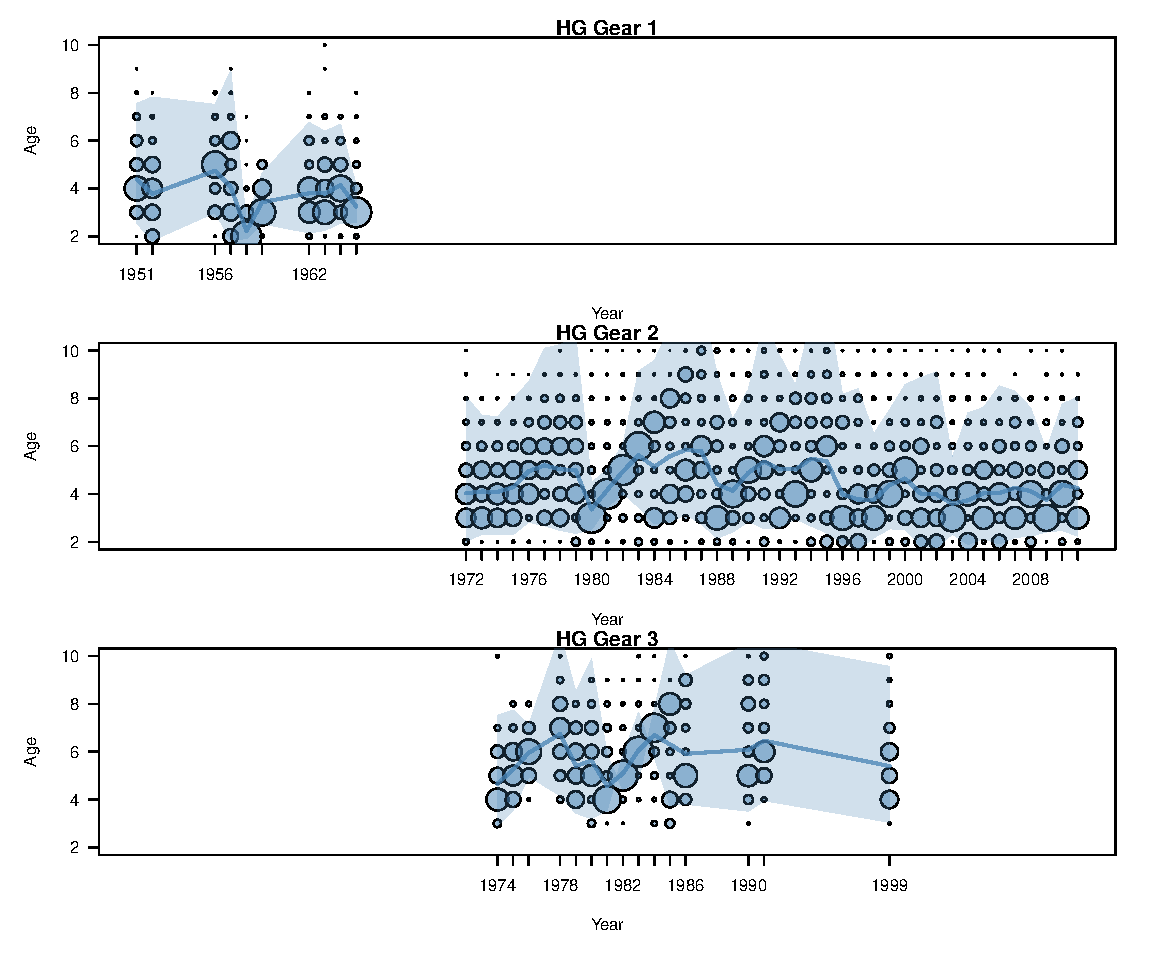
\includegraphics[width=0.85\textwidth]{../Figs/iscam_fig_AgeCompsHG.pdf}\\
	\caption{Bubble plots showing the proportions-at-age versus time for the winter purse seine fishery (top), seine roe fishery (middle) and the gillnet fishery (bottom) in Haida Gwaii.  The area of the circle is proportional to cohort abundance, each column sums to 1, zeros are not shown, and age 10 is a plus group. Also shown is the mean age of the catch (line) and the approximate 95\% distribution of ages (shaded polygon) for each year.}\label{FigAgeCompsHG}
\end{sidewaysfigure}

\begin{sidewaysfigure}[!tbp]
	% Requires \usepackage{graphicx}
	\centering
	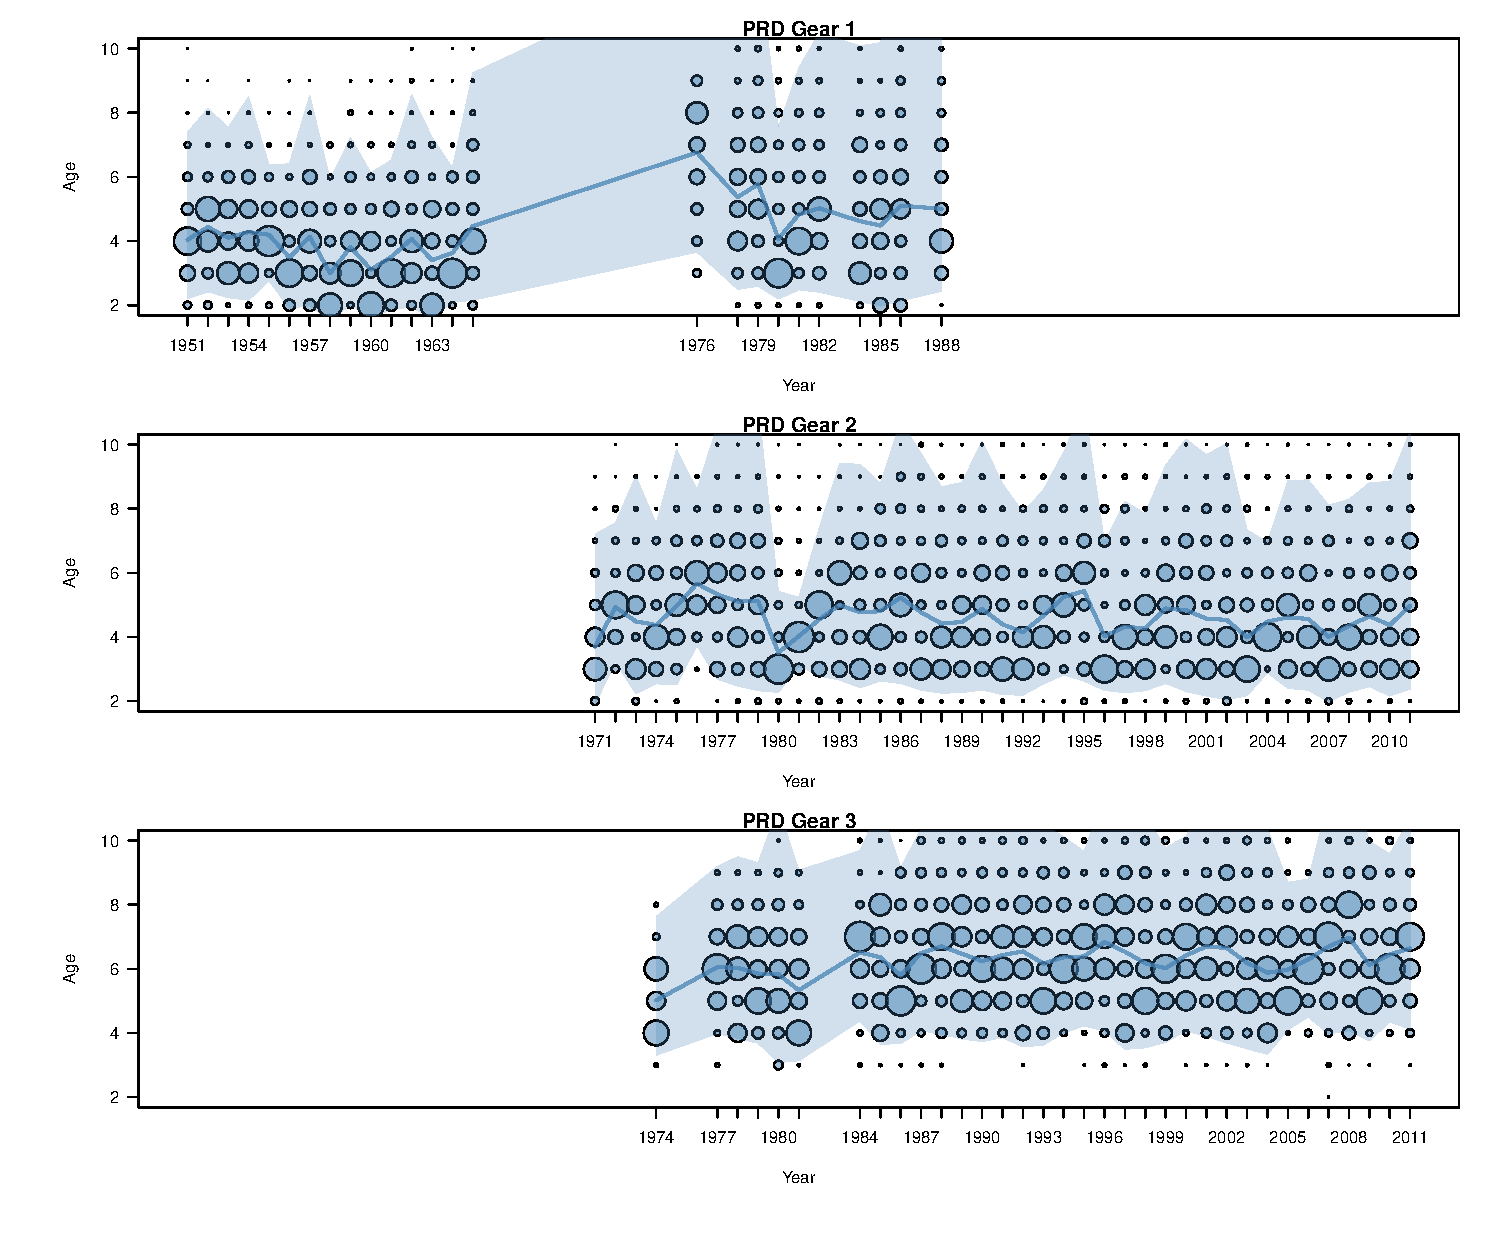
\includegraphics[width=0.85\textwidth]{../Figs/iscam_fig_AgeCompsPRD.pdf}\\
	\caption{Bubble plots showing the proportions-at-age versus time for the winter purse seine fishery (top), seine roe fishery (middle) and the gillnet fishery (bottom) in Prince Rupert District.  The area of the circle is proportional to cohort abundance, each column sums to 1, zeros are not shown, and age 10 is a plus group. Also shown is the mean age of the catch (line) and the approximate 95\% distribution of ages (shaded polygon) for each year.}\label{FigAgeCompsPRD}
\end{sidewaysfigure}

\begin{sidewaysfigure}[!tbp]
	% Requires \usepackage{graphicx}
	\centering
	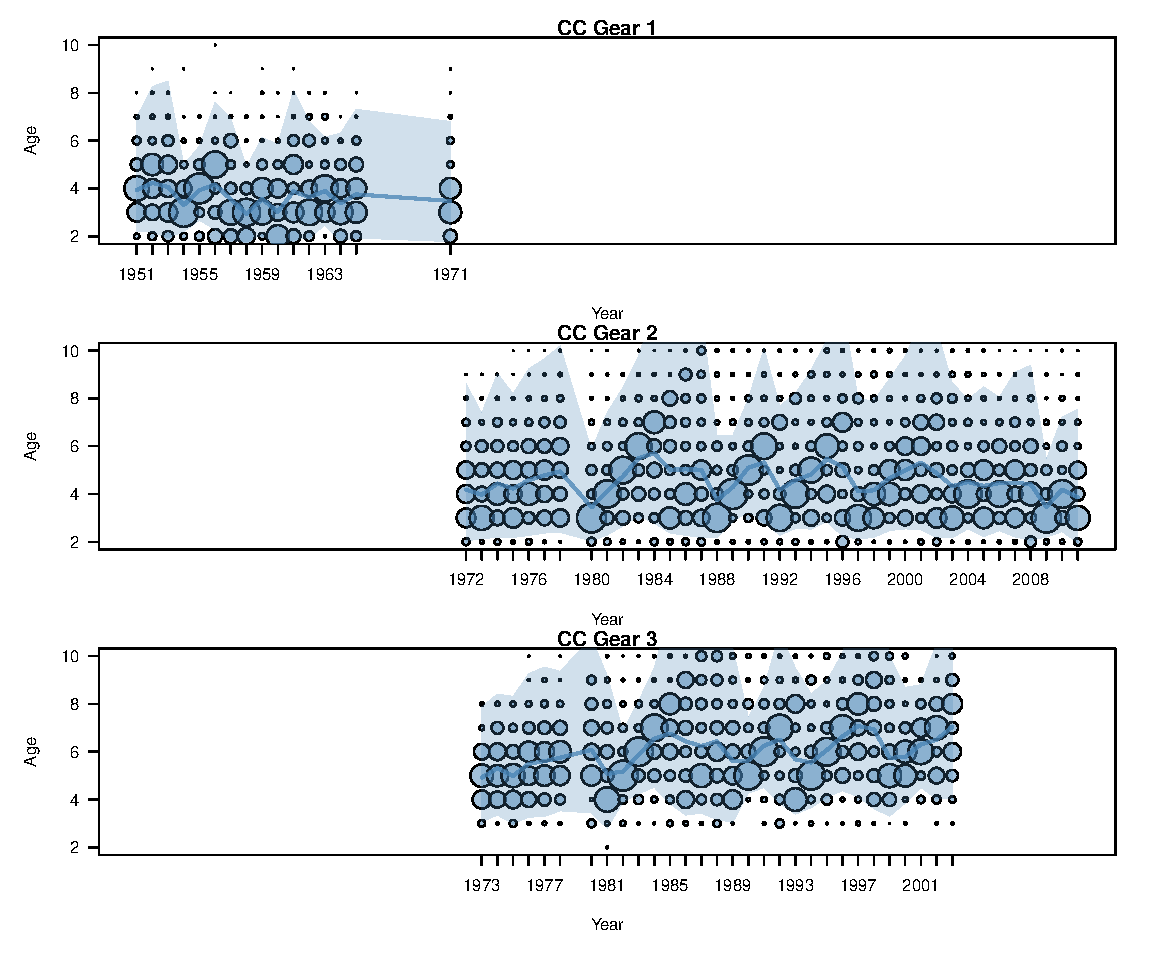
\includegraphics[width=0.85\textwidth]{../Figs/iscam_fig_AgeCompsCC.pdf}\\
	\caption{Bubble plots showing the proportions-at-age versus time for the winter purse seine fishery (top), seine roe fishery (middle) and the gillnet fishery (bottom) in the Central Coast region.  The area of the circle is proportional to cohort abundance, each column sums to 1, zeros are not shown, and age 10 is a plus group. Also shown is the mean age of the catch (line) and the approximate 95\% distribution of ages (shaded polygon) for each year.}\label{FigAgeCompsCC}
\end{sidewaysfigure}

\begin{sidewaysfigure}[!tbp]
	% Requires \usepackage{graphicx}
	\centering
	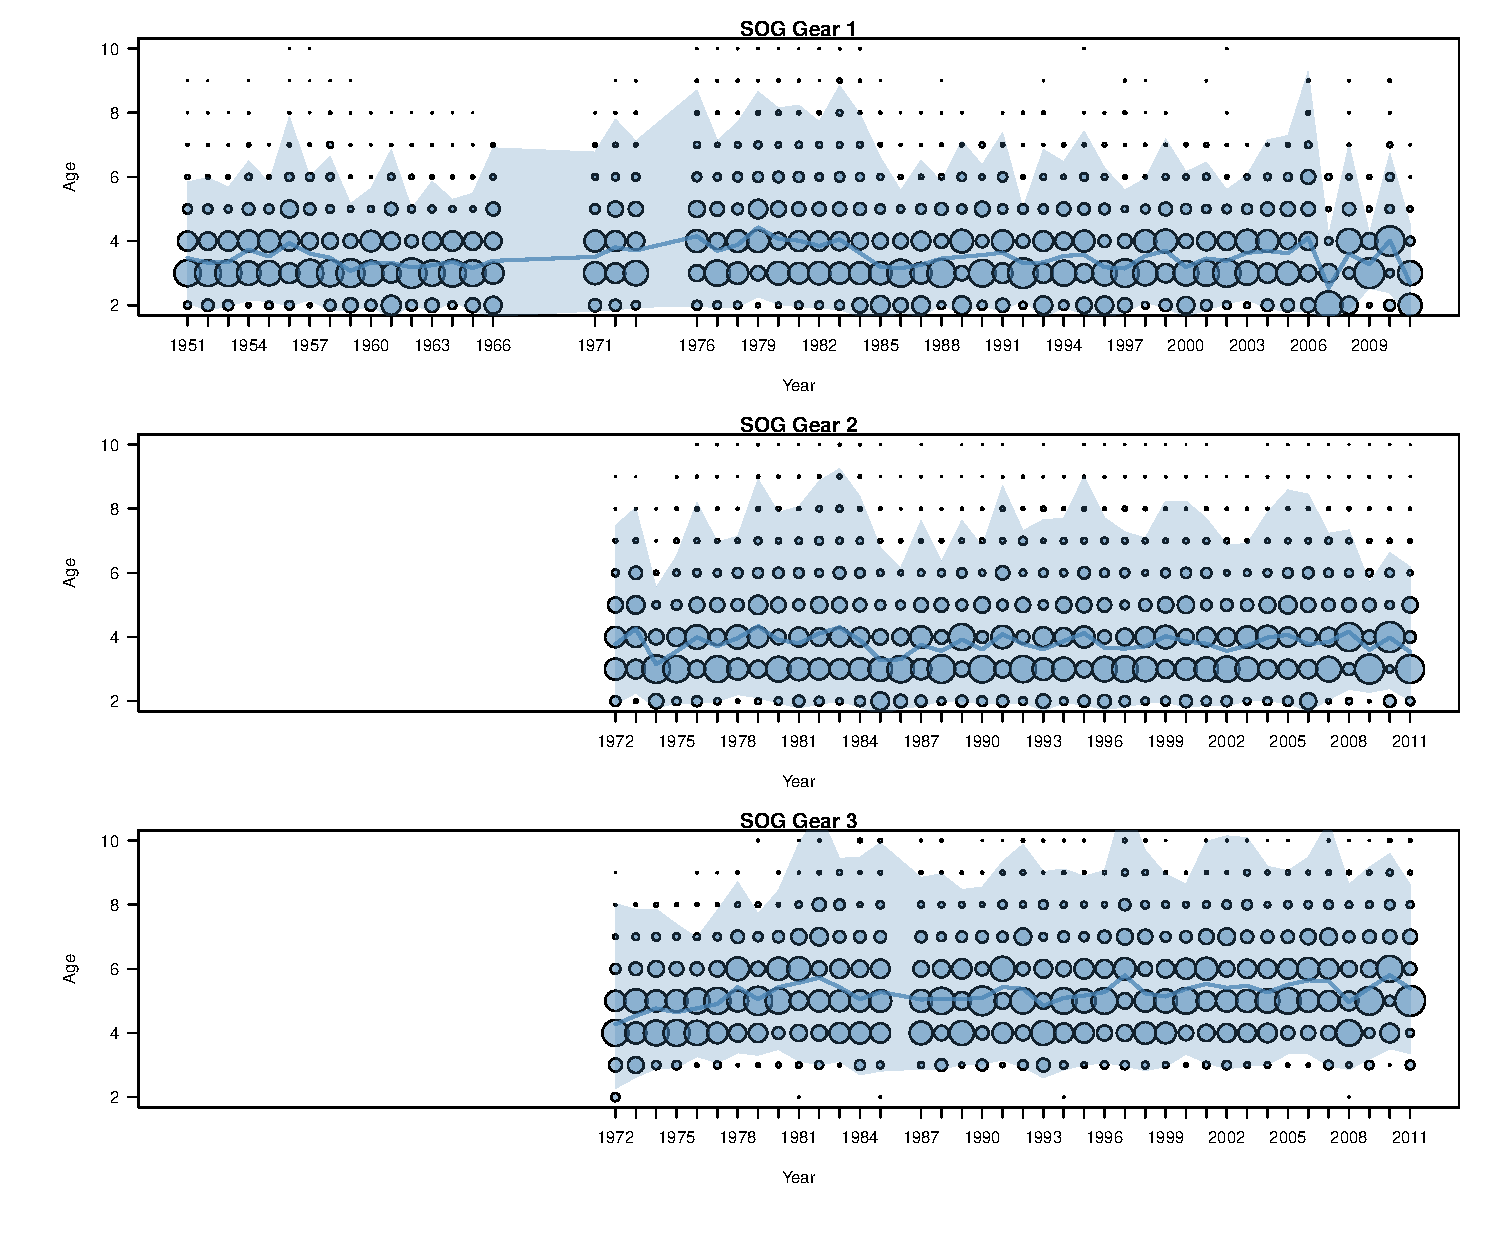
\includegraphics[width=0.85\textwidth]{../Figs/iscam_fig_AgeCompsSOG.pdf}\\
	\caption{Bubble plots showing the proportions-at-age versus time for the winter purse seine fishery (top), seine roe fishery (middle) and the gillnet fishery (bottom) in the Strait of Georgia.  The area of the circle is proportional to cohort abundance, each column sums to 1, zeros are not shown, and age 10 is a plus group. Also shown is the mean age of the catch (line) and the approximate 95\% distribution of ages (shaded polygon) for each year.}\label{FigAgeCompsSOG}
\end{sidewaysfigure}

\begin{sidewaysfigure}[!tbp]
	% Requires \usepackage{graphicx}
	\centering
	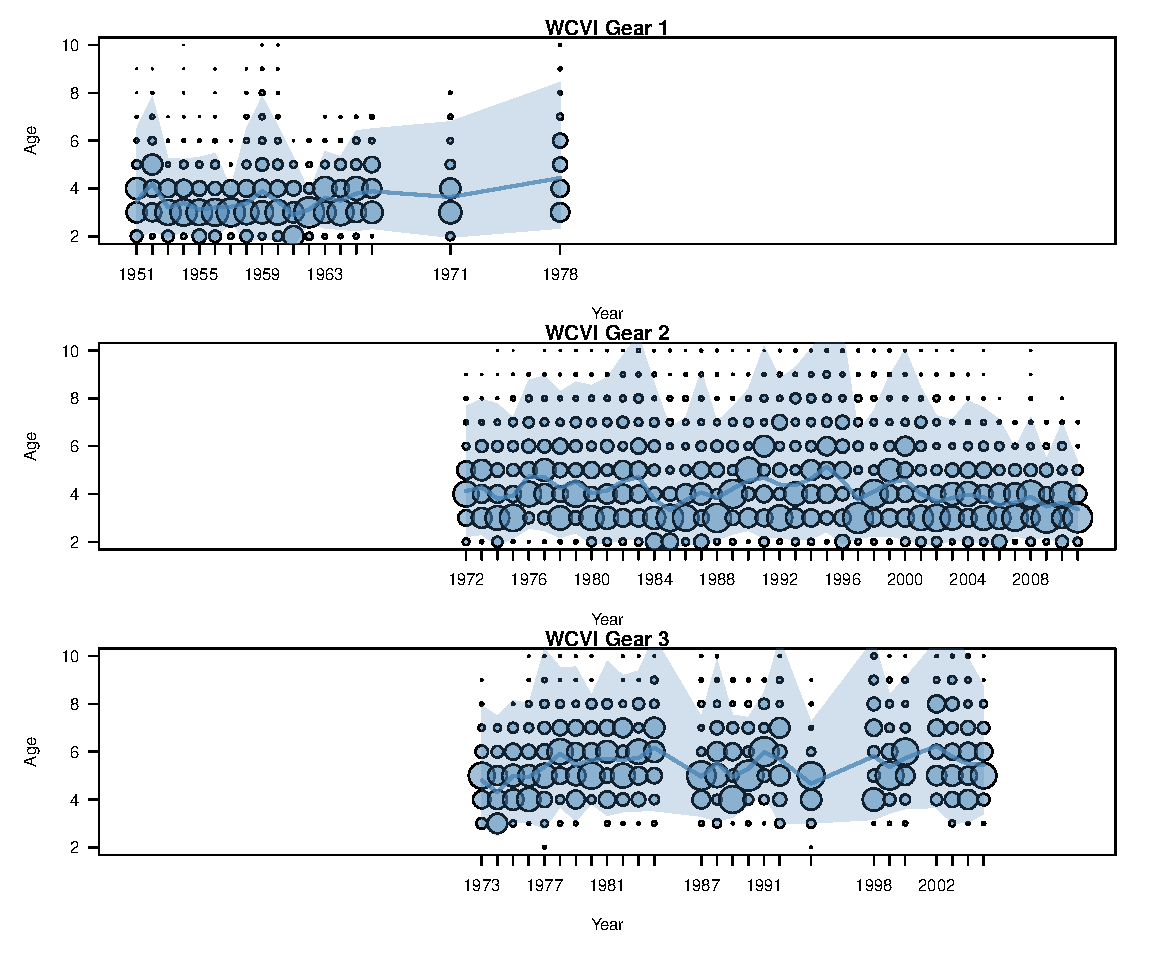
\includegraphics[width=0.85\textwidth]{../Figs/iscam_fig_AgeCompsWCVI.pdf}\\
	\caption{Bubble plots showing the proportions-at-age versus time for the winter purse seine fishery (top), seine roe fishery (middle) and the gillnet fishery (bottom) in the West Coast Vancouver Island region.  The area of the circle is proportional to cohort abundance, each column sums to 1, zeros are not shown, and age 10 is a plus group. Also shown is the mean age of the catch (line) and the approximate 95\% distribution of ages (shaded polygon) for each year.}\label{FigAgeCompsWCVI}
\end{sidewaysfigure}





	\subsubsection{Mean weight-at-age data}

	From the mid-1970s until the present, there has been a measurable decline in weight-at-age for all ages in all major stock areas (Figure \ref{FigMeanWt}). Samples collected during the 2009/10 fishing year indicate weights-at-age that are among the lowest on record. This declining weight-at-age may be attributed to any number of factors, including: fishing effects (i.e., gear selectivity), environmental effects (changes in ocean productivity), or it may even be attributed to changes in sampling protocols (shorter time frame over which samples are collected). Declining weight-at-age has been observed in all five of the major stocks, and despite area closures over the last 10-years, has continued to occur in the QCI and WCVI stocks. Although the direct cause of this decline is still to be investigated, this trend has been observed in B.C. and U.S. waters, from California to Alaska \citep{schweigert2002herring}, and merits further research.	The observed mean weight-at-age data appear to have a few  errors that need to be investigated as well; for example, see the apparently small age-10 fish in 2001 in Figure \ref{FigMeanWt}.

\begin{figure}[!tbp]
	% Requires \usepackage{graphicx}
	\centering
	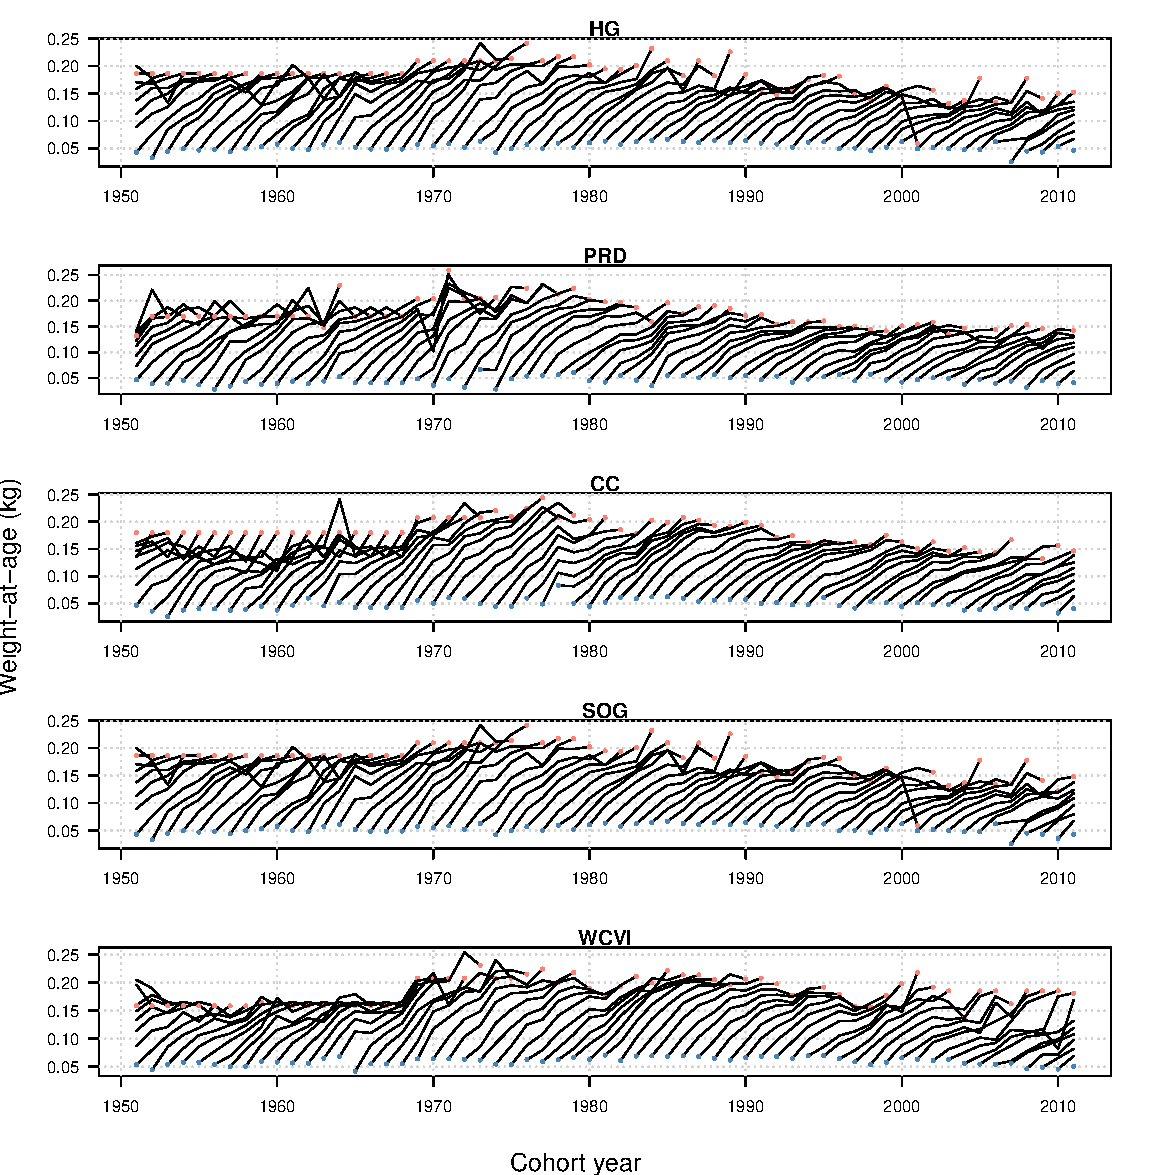
\includegraphics[width=\textwidth]{../Figs/iscam_fig_MeanWt.pdf}\\
	\caption{Empirical mean weight-at-age data by cohort from 1951 to 2011 for ages 2 to 10 in the five major Stock Assessment Regions.}\label{FigMeanWt}
\end{figure}
	

%%%%%%%%%%%%%%%%%%%%%%%%%%%%%%%%%%%%%%%%%%%%%%%%%%%%%%%%%%%%%%%%%%%%%
%%%%%%%%%%%%%%%%%%%%%%%%%%%%%%%%%%%%%%%%%%%%%%%%%%%%%%%%%%%%%%%%%%%%%
%%%%%%%%%%%%%%%%%%%%%%%%%%%%%%%%%%%%%%%%%%%%%%%%%%%%%%%%%%%%%%%%%%%%%	
	\subsection{Analytical methods}

	For the 2011 BC herring assessment, \iscam was used to conduct the stock assessment for each of the five major Stock Assessment Regions (SAR) and two minor assessment areas (Area 2W and Area 27).  The technical details of this model can be found in Appendix \ref{appiSCAM}.
		
	\subsection{Retrospective analysis}
	A retrospective analysis was conducted for each of the major and minor SARs.  The retrospective analysis successively removes the last 10-years of data and examines changes in estimates of terminal spawning biomass.  The results are then plotted on a single panel to compare how estimates of spawning biomass change as successive years of data are omitted from the analysis.
	
	\subsection{Abundance and recruitment forecasts}
	The abundance forecast for the upcoming fishing season, also referred to as pre-fishery biomass, is defined as the predicted biomass of age-4 fish and older plus the number of age-3 fish recruiting in year $T+1$.  The abundance estimates are based on the median values from the sampled posterior distribution.  Age-3 recruits are based on poor, average, and good recruitment scenarios; see next paragraph for definitions of poor, average and good.
	
	The recruitment forecasts are based on the surviving number of age-3 fish at the start of the fishing season times the average weight-at-age 3 in the last 5 years. The definitions of poor, average, and good recruitment are as follows: \textbf{Poor} is the average recruitment from the 0-33 percentile, \textbf{Average} is the average recruitment from the 33-66 percentile, and \textbf{Good} is the average recruitment from the 66-100 percentile.  Note that all cohorts from 1951 to 2011  were included in the calculation of recruitment quantiles.
	
	\subsection{Catch advice}
Catch advice is based on the application of the harvest control rule (HCR). The herring HCR has three components:
\begin{enumerate}
\item Reference points (LRP, USR, and cuttoffs)
\item Harvest rate
\item Decision rules
\end{enumerate}

For each of the five major stocks, the limit reference point (LRP) is the cuttoff value, which is defined here as 0.25\bo\, and the	Upper Stock Reference (USR) is defined as the 1.05*LRP (0.25\bo\ + 0.2*0.25\bo = LRP + 0.05LRP). \textbf{For clarification, references to \bo\ throughout this document refer to the mature spawning stock biomass.} The default harvest rate if the stock is at or above USR is 0.2, and declines linearly to 0 when the stock is at or below the LRP (a default harvest rate of 0.1 is used for the minor stock areas).  The decision rule for the major stock areas operates as follows:

\begin{itemize}
	\item If the forecast run is less than the LRP (cuttoff) then the area is closed to all commercial harvest  (i.e., stock is deemed to be in the critical zone).
	
	\item If the forecast run is greater than the LRP and less than the USR (i.e., cautious zone), then total allowable catch is based on a reduced harvest rate that would deplete the stock to the LRP level.
	
	\item If the forecast run is greater than USR, then the total allowable catch is set at 20\% of the forecast run.
\end{itemize}



	


%% SECTION Results
%!TEX root = /Users/stevenmartell/Documents/CURRENT PROJECTS/iSCAM-trunk/fba/BC-herring-2011/WRITEUP/BCHerring2011.tex
\section{Results}
The results section is broken down into three major subsections, Maximum likelihood fits to the data, marginal posterior distributions, and stock forecasts and catch advice based on samples from the joint posterior distribution.

\subsection{Maximum likelihood fits to the data}
Although  the maximum likelihood estimates are not explicitly used for constructing the catch advice, we do present the MLE estimates of the residual patterns and fits to the data for comparisons.

\subsubsection{Catch residuals}
Residuals between the observed and predicted catch are largely determined by the user specified standard deviation in each of the control files.  In this assessment, the assumed variance for all regions (including minor regions) was set at 0.005, which corresponds to a standard deviation of approximately 0.0707.  Overall the residuals for each fishery in each stock assessment region are unremarkable (Fig. \ref{PartII:Results:fig1}), with exception of a  major outlier in the Haida Gwaii in the mide 1950s.  In 1956, the reported catch in Haida Gwaii was extremely large ($>$ 60,000 mt) and the model has a difficult time explaining this large catch. In order to explain this large catch in a single year, a large biomass in the region is required.

\begin{figure}[!tbp]
	% Requires \usepackage{graphicx}
	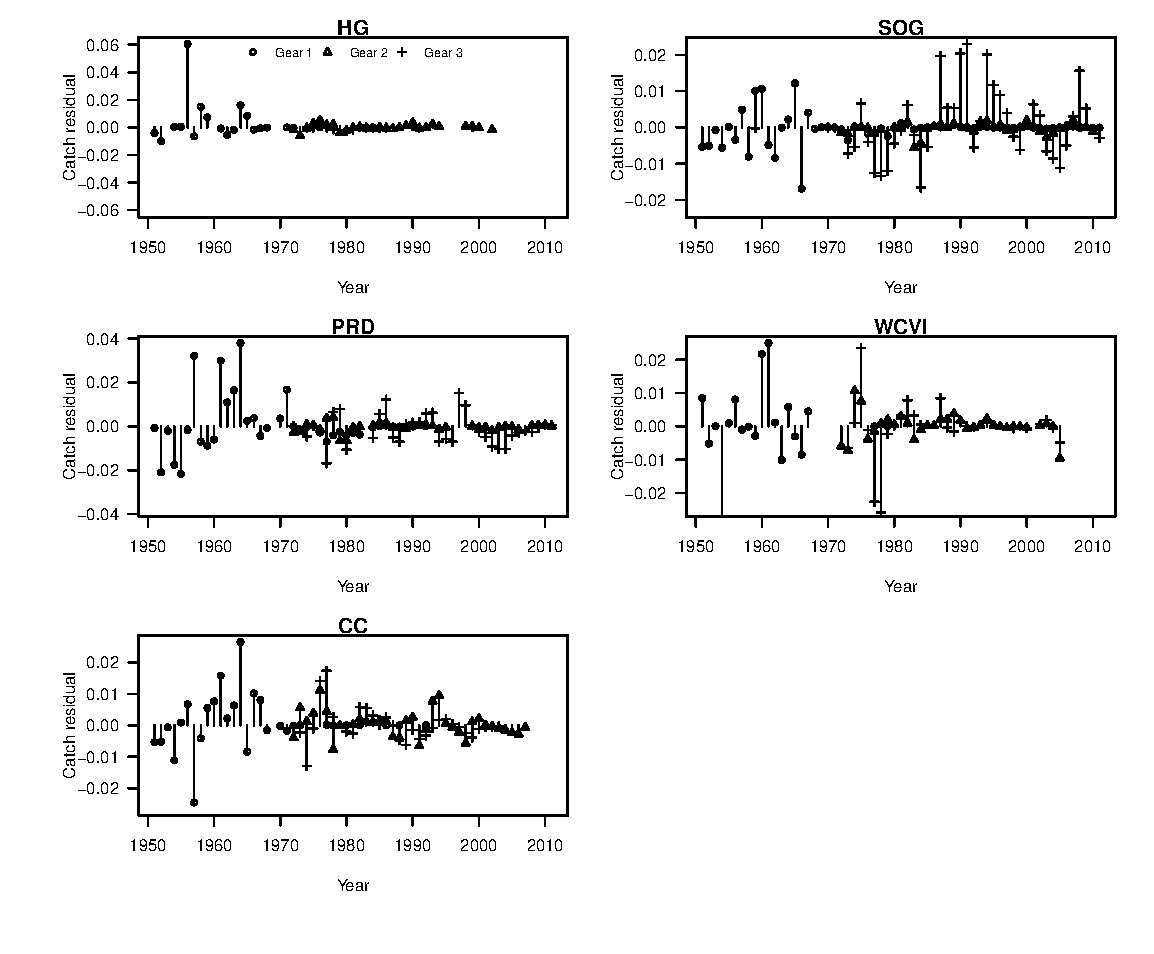
\includegraphics[width=\textwidth]{../FIGS/qPriorFigs/iscam_fig_catchresid.pdf}\\
	\caption{Residual for the log difference between observed and predicted catch for the five major SARs for each gear type (Gear 1 = winter seine fishery, Gear 2 = seine-roe fishery, Gear 3 = gill net fishery).}\label{PartII:Results:fig1}
\end{figure}


\subsubsection{Fits to the spawn survey data}
The residuals between the observed and predicted spawn survey index (on a log scale) are shown in Figure \ref{PartII:Results:fig2}.  Recall that the spawn survey data are treated as two independent time series where data between 1951--1987 were based on surface estimates of spawn area and data post 1988 are based on diver surveys of spawn area.  More weight was assigned to the contemporary data.   

For most areas, there is little pattern in the residuals between the observed and predicted survey data (Fig \ref{PartII:Results:fig2}).  For the HG, PRD and CC regions, there is very good correspondence between the observed and predicted survey data post 1988.  IN the SOG, there is a period of positive residuals between 1999 and 2005 where the predicted spawn biomass fails to increase as much as indicated by the survey.  Similary 3--4 year trends also exist in the WCVI spawn survey data after the year 2000.

\begin{figure}[!tbp]
	% Requires \usepackage{graphicx}
	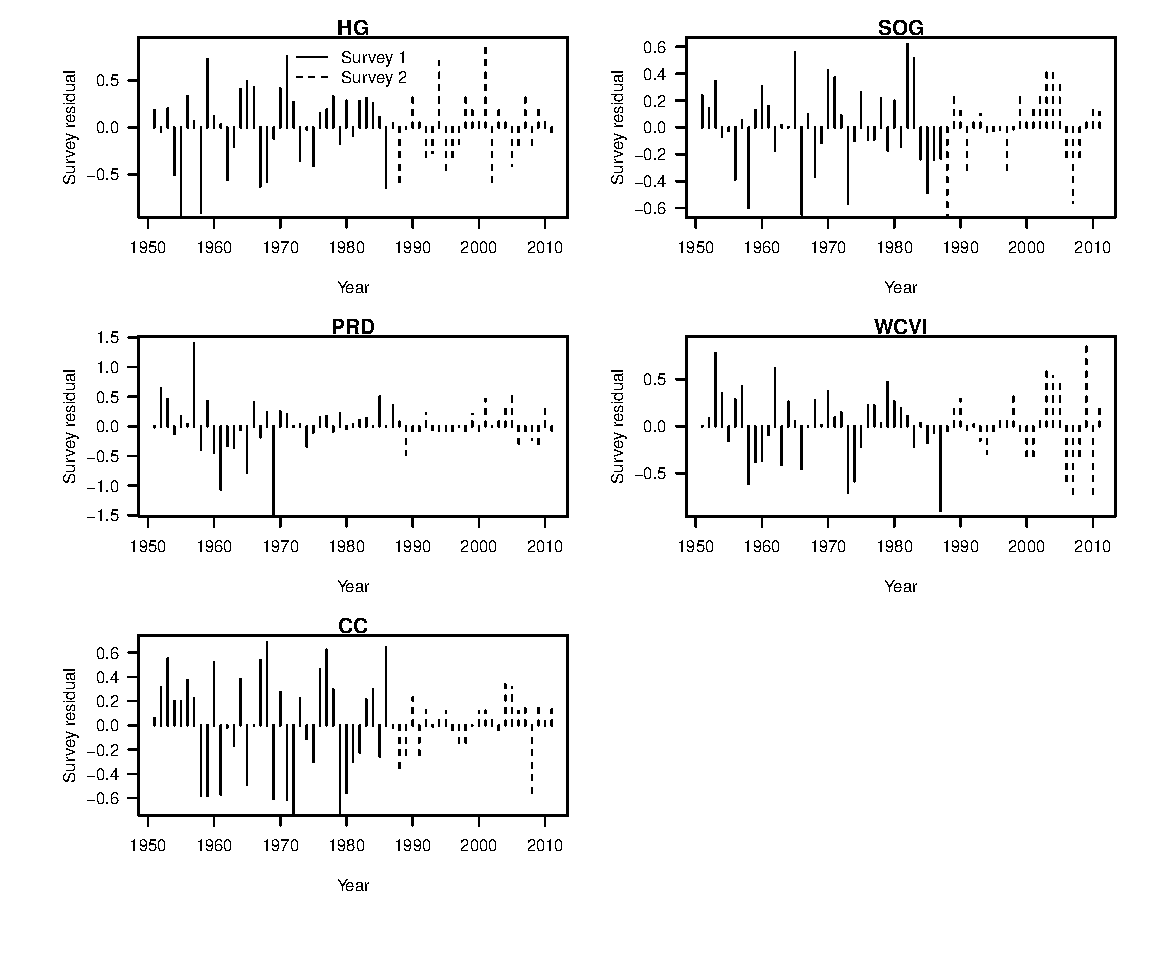
\includegraphics[width=\textwidth]{../FIGS/qPriorFigs/iscam_fig_surveyresid.pdf}\\
	\caption{Residual patterns for the log difference between observed and predicted spawn survey abundance for the five major SARs. Spawn survey data based on surface estimates are show as solid lines and data based on diver surveys is shown as dashed lines.}\label{PartII:Results:fig2}
\end{figure}

In comparison to the previous assessment for Pacific herring using the HCAM model, estimates of the catchability coefficient are very different (HCAM assumed q=1 for post 1988 data).  In each of the five major assessment regions (and the two minor regions) a less informative prior for the catchability coefficient was used (see Appendix \ref{Appendix::q_prior}).  Maximum Likelihood Estimates (MLE) of the catchability coefficients are presented for each region in Fig. \ref{PartII:Results:fig3} along with the observed and predicted trends in the spawn index.  Estimates of $q$ in both time periods are less than 1.0 for all regions with the exception of post 1988 data in the PRD region.  The interpretation of $q=1$ is that the spawn survey data is an absolute measure of spawn abundance, $q<1$ implies that the survey under-estimates the spawn abundance and $q>1$ implies an over-estimate.  For example, in the HG region the MLE values for $q$ are 0.245 and 0.433 for the pre- and post-1988 data, respectively. This could be interpreted as the spawn survey only, on average, sees 24.5\% and 43.3\% of the deposited spawn each year.  This interpretation however is conditional on the specification of mature biomass in the stock assessment model. 

\begin{figure}[!tbp]
	% Requires \usepackage{graphicx}
	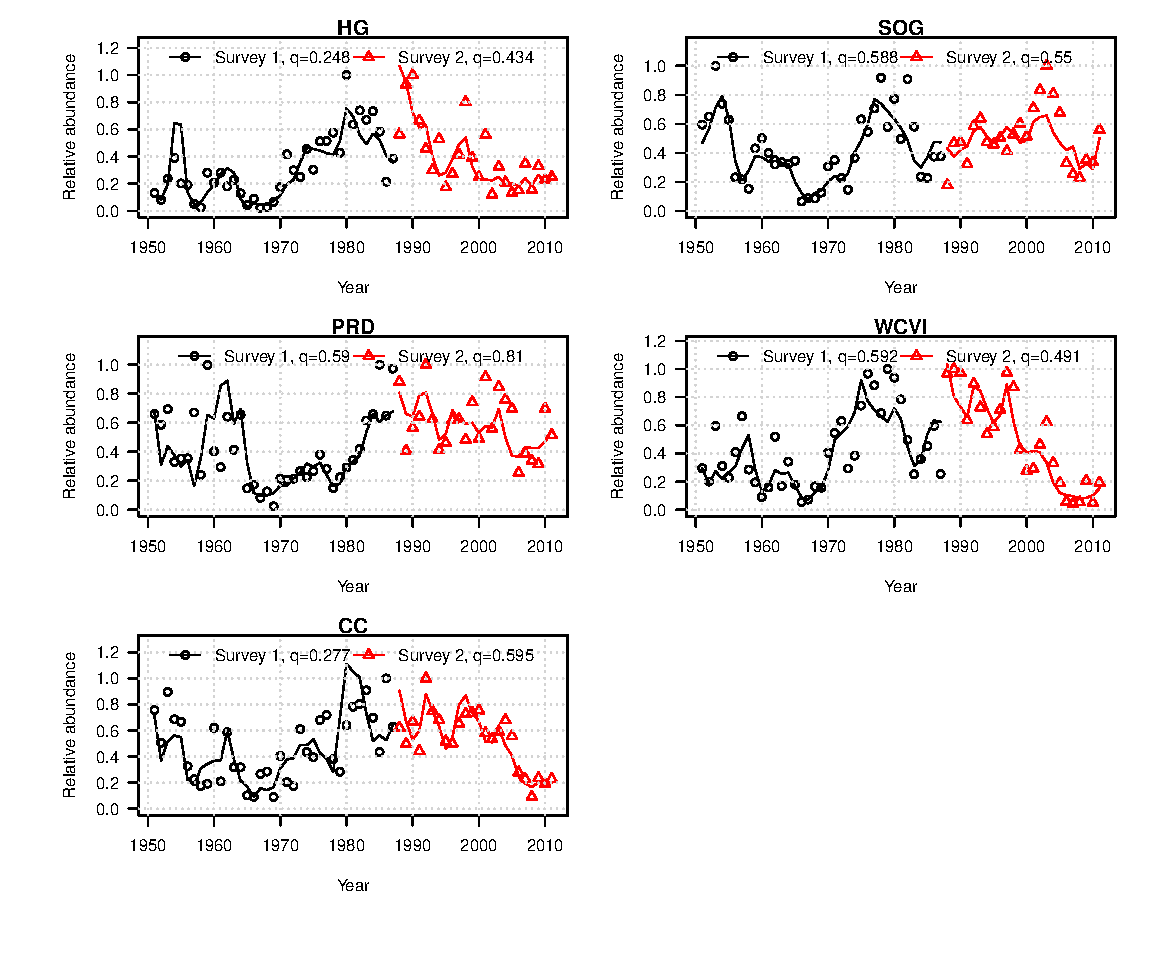
\includegraphics[width=\textwidth]{../FIGS/qPriorFigs/iscam_fig_surveyfit.pdf}\\
	\caption{Observed (points) and predicted (lines) relative abundance data (spawn survey data) for each of the five major SARs.  In each panel, the corresponding scaler ($q$) is presented for each of the surveys.}\label{PartII:Results:fig3}
\end{figure}


\subsubsection{Age composition residuals}

The assumed error distribution for the age-composition data has changed in this assessment from a multinomial distribution implemented in HCAM to a multivariate-logistic distribution. In the former implementation the age-composition data were weighted by the annual samples sizes in each region for each age and year. In the \iscam\ implementation the age-composition data for all years is given the same weight (i.e., we assume the observation errors is homogenous) based on the conditional maximum likelihood estimate of the variance (see Appendix \ref{appiSCAM} for full details).  We further pool age-proportions that are less than 2\% into the adjacent younger year class to reduce the influence of small outliers and weak cohorts.

In HG the MLE estimates of the variance for each gear is 0.102, 0.104 and 0.351, for the winter seine, seine-roe and gill net fleets, respectively (Fig. \ref{PartII:Results:figAgeCompHG}).  In general there is fairly good agreement between the observed and predicted age-composition data in this region, with poorer fits to the gill net age-composition data.  There is no persistent pattern in the residuals. 

\begin{sidewaysfigure}[!tbp]
	% Requires \usepackage{graphicx}
	\centering
	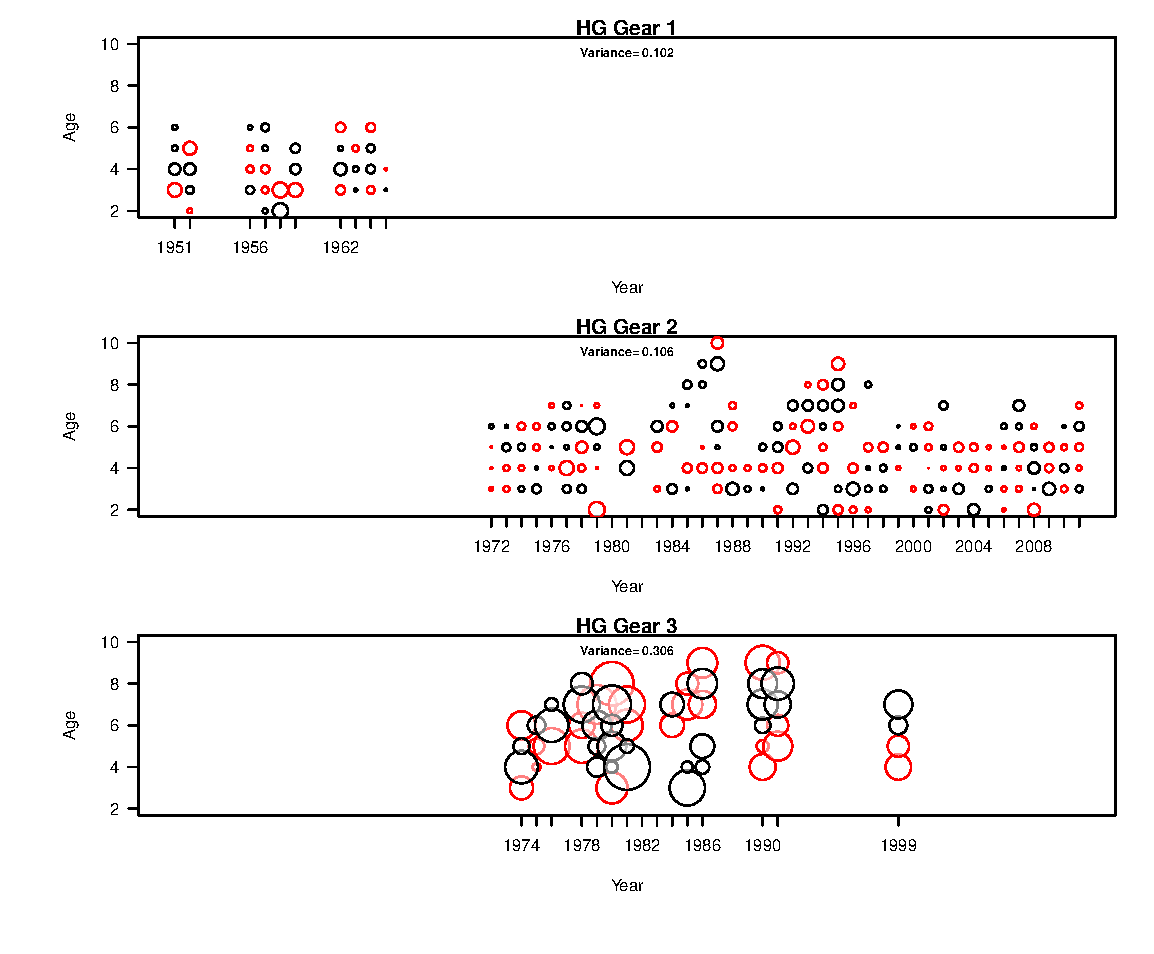
\includegraphics[width=0.9\textwidth]{../FIGS/qPriorFigs/iscam_fig_agecompsresid_HG.pdf}\\
	\caption{Residual difference between the observed and predicted proportions-at-age for HG for each of the three gear types (Gear 1 = winter seine, Gear 2 = seine-roe, Gear 3 = gill net).  The area of each circle is proportional to the residua, black is positive, and red is negative.  The corresponding MLE estimates of the residual variance is displayed in each panel.}\label{PartII:Results:figAgeCompHG}
\end{sidewaysfigure}

For the PRD region, the fits to the age-composition data are slightly poorer, with MLE estimates of the variance ranging from 0.215 to 0.358 for the seine-roe and gill net fleets (Fig. \ref{PartII:Results:figAgeCompPRD}). There is no remarkable pattern in the winter seine fishery, the seine-roe fishery tends to have positive residuals for age-3 and age 7+ fish, and negative residuals for ages 4-6 fish.  Similarly, the is an age-pattern in the residuals for the gill net fishery with negative residuals for age-4 and ages 9+ fish, and positive residuals for ages 5-8.  Residuals in 2011 age-composition data are much larger  than all other years.

\begin{sidewaysfigure}[!tbp]
	% Requires \usepackage{graphicx}
	\centering
	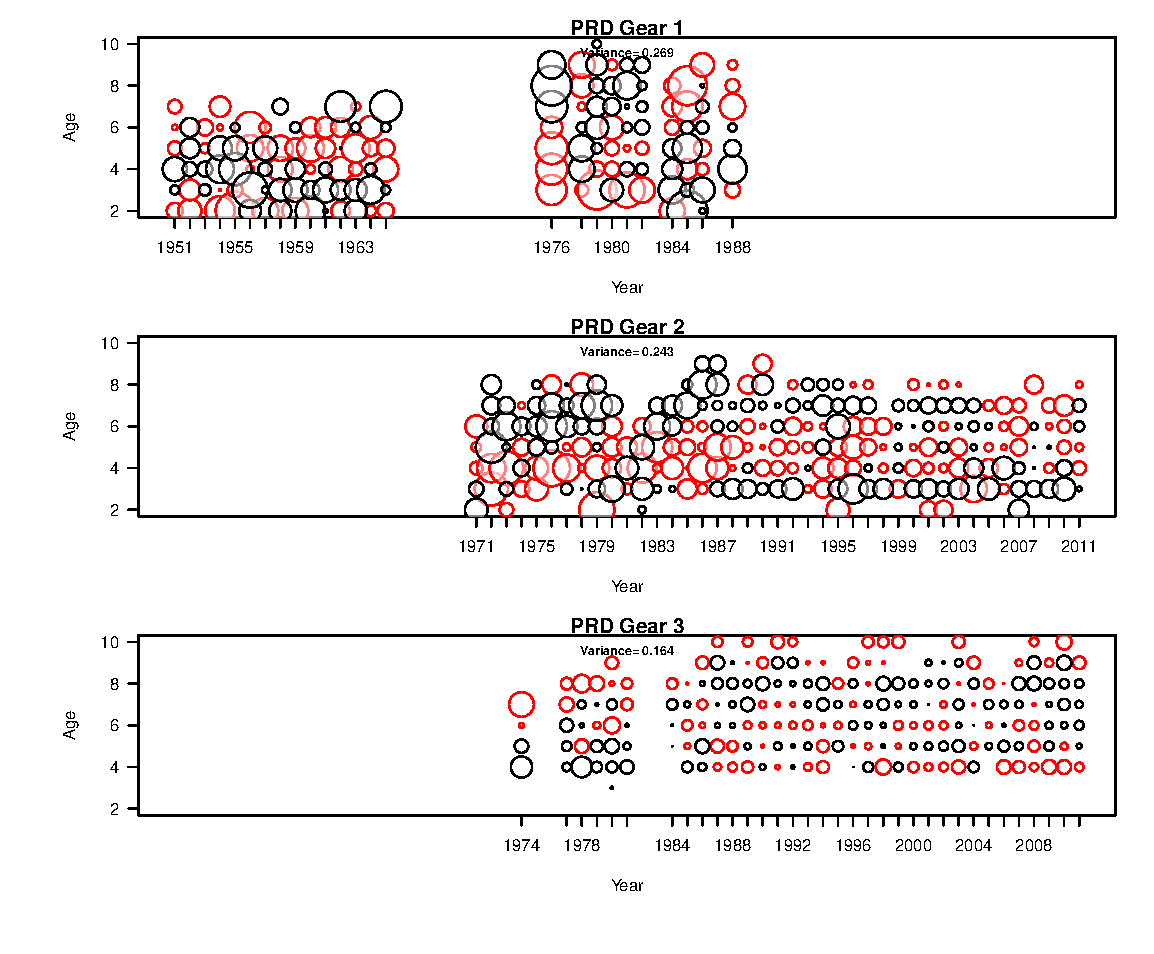
\includegraphics[width=0.9\textwidth]{../FIGS/qPriorFigs/iscam_fig_agecompsresid_PRD.pdf}\\
	\caption{Residual difference between the observed and predicted proportions-at-age for PRD for each of the three gear types (Gear 1 = winter seine, Gear 2 = seine-roe, Gear 3 = gill net).  The area of each circle is proportional to the residua, black is positive, and red is negative.  The corresponding MLE estimates of the residual variance is displayed in each panel.}\label{PartII:Results:figAgeCompPRD}
\end{sidewaysfigure}


For the Central Coast (CC) region, there is also good correspondence between the observed and predicted age-composition data, with MLE estimates of the variance ranging from 0.128 to 0.203 (Fig. \ref{PartII:Results:figAgeCompCC}).  There is no striking temporal pattern in the residuals for any of the fishing fleets.  There is a tendency to overestimate the porportion-at-age 4 and 5 in the seine-roe fishery.


\begin{sidewaysfigure}[!tbp]
	% Requires \usepackage{graphicx}
	\centering
	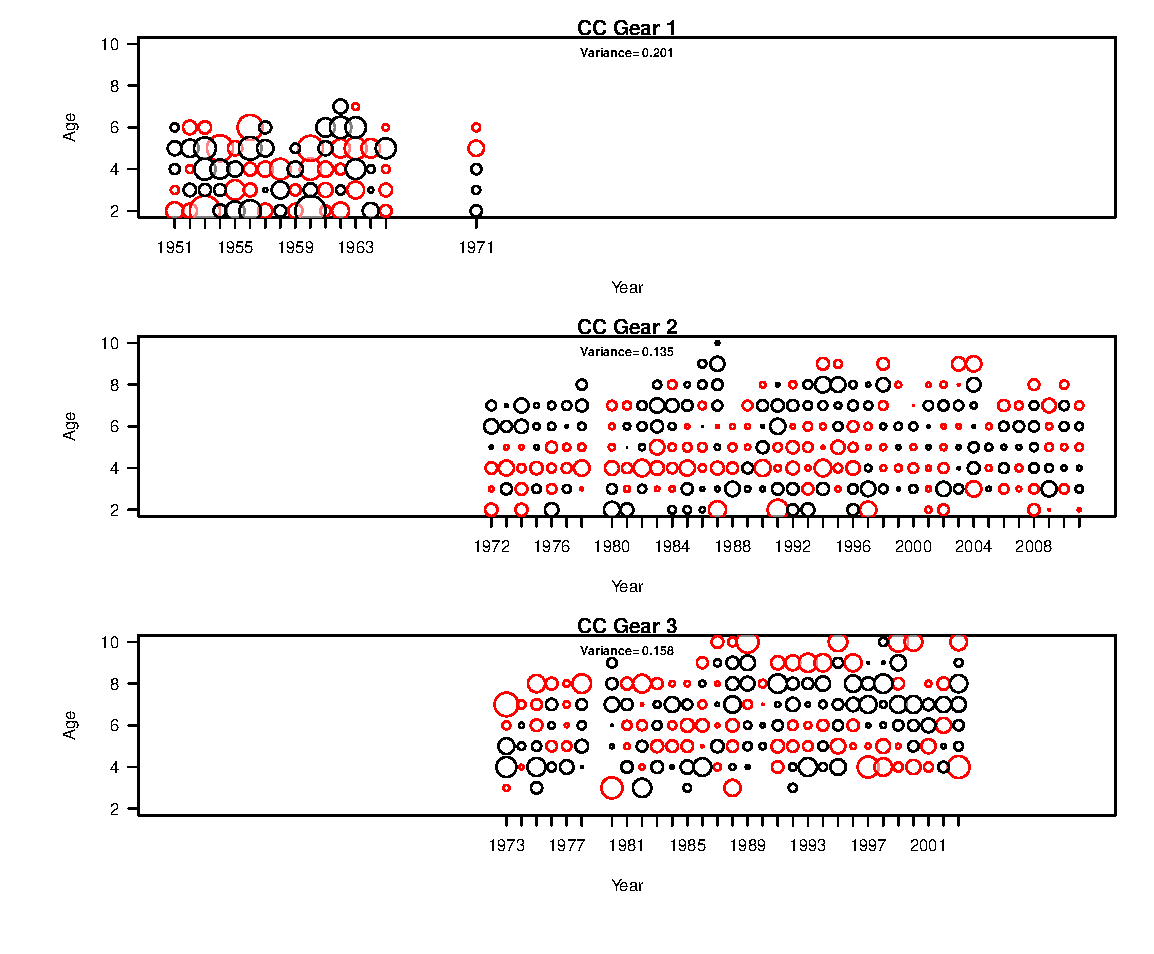
\includegraphics[width=0.9\textwidth]{../FIGS/qPriorFigs/iscam_fig_agecompsresid_CC.pdf}\\
	\caption{Residual difference between the observed and predicted proportions-at-age for CC for each of the three gear types (Gear 1 = winter seine, Gear 2 = seine-roe, Gear 3 = gill net).  The area of each circle is proportional to the residua, black is positive, and red is negative.  The corresponding MLE estimates of the residual variance is displayed in each panel.}\label{PartII:Results:figAgeCompCC}
\end{sidewaysfigure}

For the Strait of Georgia, there is also very good correspondence between the observed and predicated age-composition data for all three gears (Fig \ref{PartII:Results:figAgeCompSOG}).  The MLE estimates of the variance range from 0.088 to 0.021 for the seine-roe and gill net fleets, respectively.  In the gill net fleet  there has been a tendency to under-estimate the proportions-at-age 4-6 between the 1970s and mid 1990s and more recently to over-estimate the proportions-at-age 6-8.  Recall that selectivity for the gill net fishery is a function of the empirical weight-at-age data, which has been trending to small fish in recent years.


\begin{sidewaysfigure}[!tbp]
	% Requires \usepackage{graphicx}
	\centering
	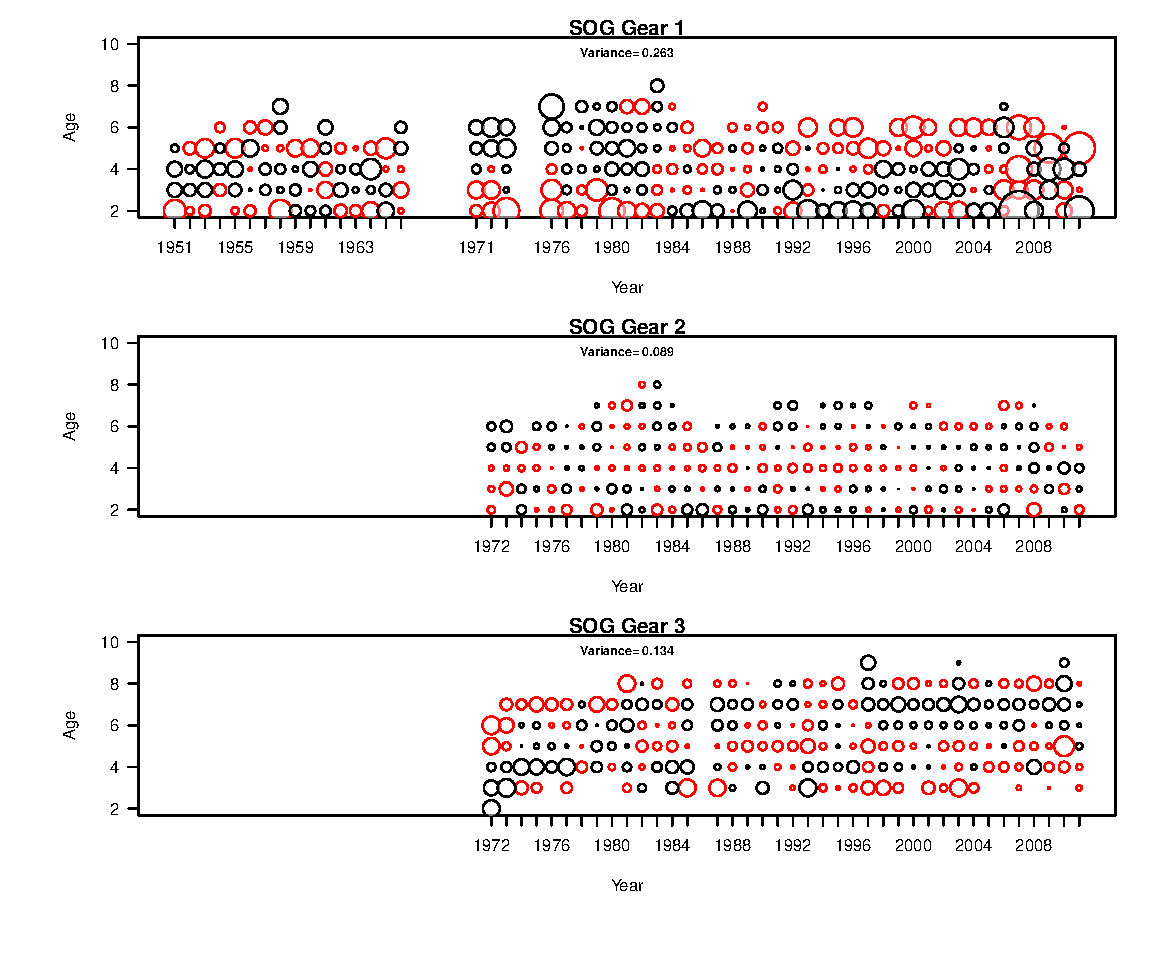
\includegraphics[width=0.9\textwidth]{../FIGS/qPriorFigs/iscam_fig_agecompsresid_SOG.pdf}\\
	\caption{Residual difference between the observed and predicted proportions-at-age for SOG for each of the three gear types (Gear 1 = winter seine, Gear 2 = seine-roe, Gear 3 = gill net).  The area of each circle is proportional to the residua, black is positive, and red is negative.  The corresponding MLE estimates of the residual variance is displayed in each panel.}\label{PartII:Results:figAgeCompSOG}
\end{sidewaysfigure}

In the case of WCVI, there is good correspondence between the observed and predicted age composition data for the seine fisheries and less so for the gill net fishery (Fig \ref{PartII:Results:figAgeCompWCVI}).  The MLE estimates of the variance range fro 0.088 to 0.314 for the seine-roe and gill net fisheries, respectively.  Residual patterns in the seine fisheries are unremarkable, perhaps an age-pattern in the seine roe fishery.  There is a tendency to under-estimate the proportions-at-age in the gill net fishery for ages 5-7.   The size of the residuals are fairly homogenous over time for all gears.


\begin{sidewaysfigure}[!tbp]
	% Requires \usepackage{graphicx}
	\centering
	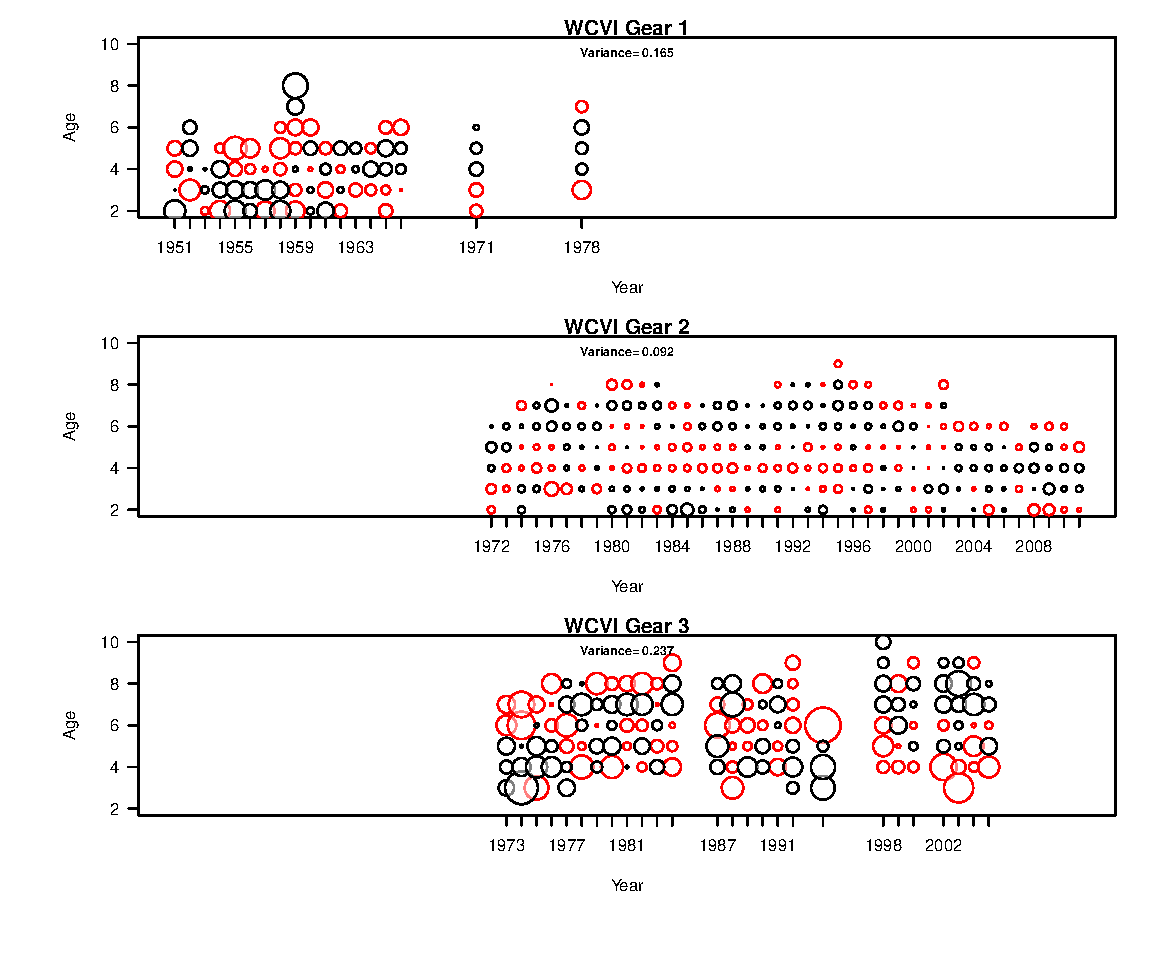
\includegraphics[width=0.9\textwidth]{../FIGS/qPriorFigs/iscam_fig_agecompsresid_WCVI.pdf}\\
	\caption{Residual difference between the observed and predicted proportions-at-age for WCVI for each of the three gear types (Gear 1 = winter seine, Gear 2 = seine-roe, Gear 3 = gill net).  The area of each circle is proportional to the residua, black is positive, and red is negative.  The corresponding MLE estimates of the residual variance is displayed in each panel.}\label{PartII:Results:figAgeCompWCVI}
\end{sidewaysfigure}







\subsubsection{Biomass estimates \& reference points}

Maximum likelihood estimates of total biomass (age 2+) and the spawning stock biomass for each of the five major assessment regions in summarized in Figure \ref{PartII:Results:figBiomass}.  Estimates of spawning stock depletion ($B_t/B_0$) for the five major regions is summarized in Figure \ref{PartII:Results:figDepletion} along with estimates of the sustainable fisheries framework reference points.  With the exception of the SOG, estimates of spawning stock depletion in 2011 are all currently below 40\% of their estimated unfished state, and in PRD, CC and the WCVI  are all estimated to be below 25\% of their unfished state (Fig \ref{PartII:Results:figDepletion}).

Spawning stock biomass in 2011 was estimated as follows: HG -- 16,789 tonnes, PRD -- 18,170 tonnes, CC -- 11,077 tonnes, SOG -- 72,135 tonnes, and WCVI -- 11,764 tonnes (Table \ref{PartII:Table1:referencePoints}).  With the exception of the PRD, these estimates are considerably higher in comparison to last years HCAM estimates; the difference largely owes to the substantial change in spawn survey scaling coefficient ($q$).

In addition to the current estimates of spawning biomass, Table \ref{PartII:Table1:referencePoints} also summarizes estimates of reference points and the total number of estimated parameters for each of the five major stock assessment regions.  Each region contained data from 1951 to 2010, and the number of estimated parameters ranges from 158 in HG to 234 in SOG.  The difference in the number of estimated parameters owes to the difference in the number of years of catch data for each region.

Estimates of unfished spawning biomass for each region is as follows: HG -- 40,960 tonnes, PRD -- 80,247 tonnes, CC -- 56,181 tonnes, SOG --- 116,023 tonnes, and WCVI -- 51,379 tonnes.  Applying the same cuttoff rule used in previous assessments (25\% of $B_0$), the results in a substantial change in the cuttoff levels for PRD, CC, SOG, and WCVI.  The previous cuttoff level for HW was estimated at 10,700 tonnes, and in this assessment there is a minor downward revision to 10,240 tonnes.  In the case of PRD, the previous cuttoff was 12,100 tonnes and in this assessment is now 20,062 tonnes.  For the CC, the previous cuttoff was 17,600 tonnes and now 14,045 tonnes.  For the SOG, the previous cuttoff was 21,200 tonnes, and in this assessment it has been revised upwards to 29,006 tonnes.  Lastly, for the WCVI the cuttoff has decreased from 18,800 tonnes to 12,845 tonnes.


% latex.default(rpTable, file = fn, title = "Stock", longtable = FALSE,      landscape = FALSE, cgroup = NULL, n.cgroup = NULL, caption = cap,      label = "TableRefPoints", na.blank = TRUE, vbar = FALSE,      size = "small") 
%
\begin{table}[!tbp]
 \small
 \caption{Summary of maximum likelihood estimates for  the 
	two minor stock areas.  No. is the total number of estimated 
	parameters, \fmsy\ the average instantaneous fishing rate to 
	achieve the maximum sustainable yield (MSY), \bo\ is the unfished 
	spawning biomass, \bmsy\ is the spawning biomass that achieves 
	maximum sustainable yield,$B_t$ is the spawning biomass at the end 
	of the 2011 fishing season, and $B_t/B_0$ is the spawning depletion 
	level at the end of the 2011 fishing season.\label{TableRefPoints}} 
 \begin{center}
 \begin{tabular}{lll}\hline\hline
\multicolumn{1}{l}{Stock}&\multicolumn{1}{c}{A2W}&\multicolumn{1}{c}{A27}\tabularnewline
\hline
No.&74&79\tabularnewline
\fmsy& 0.34&  1.9\tabularnewline
MSY&  265&  304\tabularnewline
$B_0$&2,915&2,084\tabularnewline
0.25$B_0$&  729&  521\tabularnewline
\bmsy&  705&  447\tabularnewline
0.8\bmsy&  564&  358\tabularnewline
0.4\bmsy&  282&  179\tabularnewline
$B_t$&4,671&  924\tabularnewline
$B_t/B_0$&  1.6& 0.44\tabularnewline
\hline
\end{tabular}

\end{center}

\end{table}




\begin{figure}[!tbp]
	% Requires \usepackage{graphicx}
	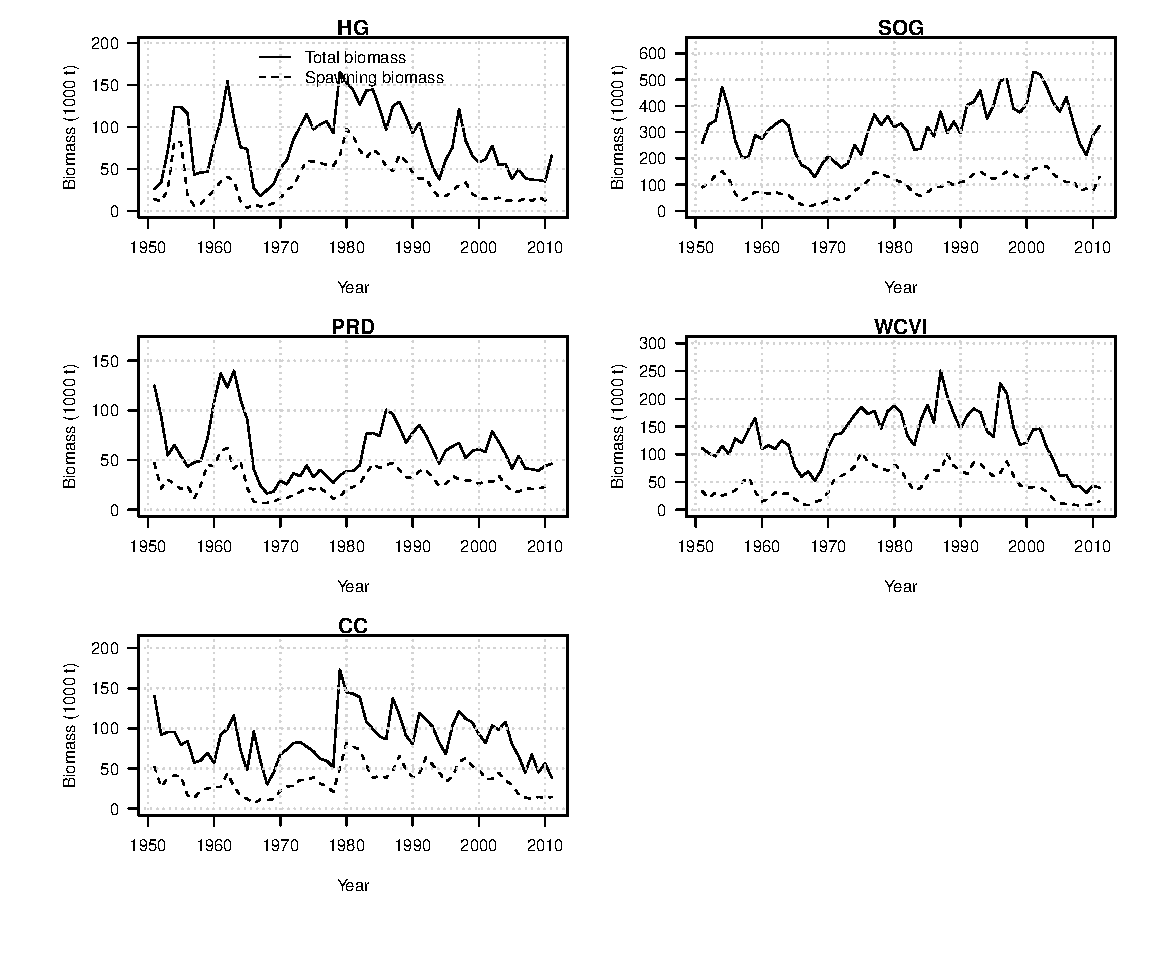
\includegraphics[width=\textwidth]{../FIGS/qPriorFigs/iscam_fig_biomass.pdf}\\
	\caption{Estimates of total biomass at the start of the year (numbers times empirical weight-at-age) and spawning stock biomass (post fishery) for the five major SARs.}\label{PartII:Results:figBiomass}
\end{figure}


\begin{figure}[!tbp]
	% Requires \usepackage{graphicx}
	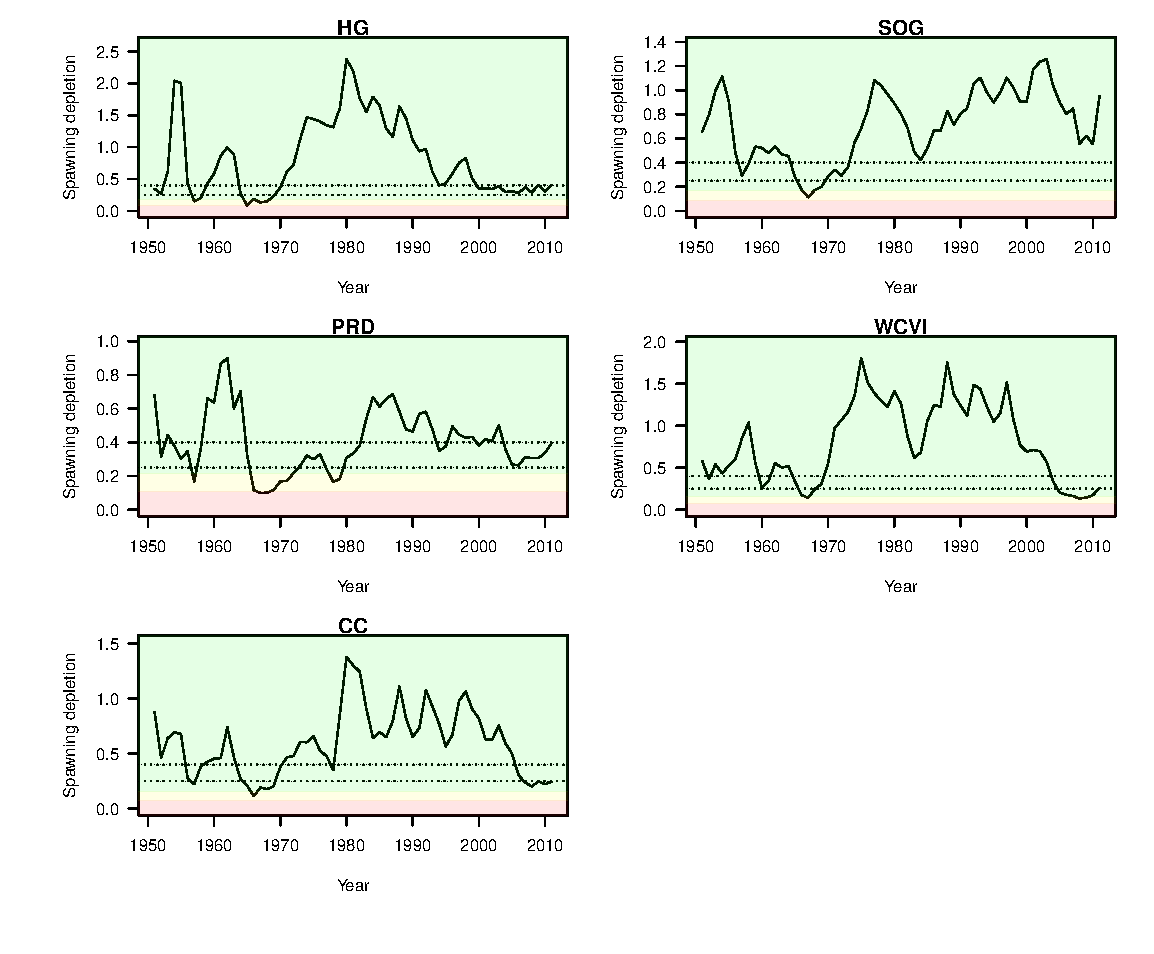
\includegraphics[width=\textwidth]{../FIGS/qPriorFigs/iscam_fig_depletion.pdf}\\
	\caption{Estimates of spawning biomass depletion ($B_t/B_0$) for each of the five major stock areas.  Horizontal dotted lines represent 25\% and 40\% depletion levels, and the shaded regions demarcate reference points based on $<$40\% \bmsy/\bo (critical zone) and 40--80\% \bmsy/\bo(cautious zone) and $>$80\% \bmsy/\bo (healthy zone).}\label{PartII:Results:figDepletion}
\end{figure}




\subsubsection{Estimates of mortality}

The most recent HCAM assessment model allowed for annual estimates of $M_t$ where natural mortality was modelled as a random walk process.  The same random walk model has been adopted in this \iscam\ implementation, however, a reduced number of parameters (12 nodes instead of 60 annual deviations) is estimated and interpolated using a bicubic spline.  The number of estimated nodes does have minor influences on the various trends in natural mortality; we came to arrive at estimating 12 nodes by ensuring the estimated trends were very similar to trends in $M$ when estimated annual natural mortality rates (NB. one could use formal model selection criterion here to determine the optimal number of nodes).

For all of the five major stock assessment regions, estimates of natural mortality rates have trended upwards since the 1950s (Figure \ref{PartII:Results:figMortality}).  Trends in estimates of natural mortality are also consistent with the trends in natural mortality from last years HCAM model  \citep[see Figure 18 in][]{Clear2010}.  In the mid to late 1970s, estimates of natural mortality rates were very low during a time when most of the stocks were recovering from the earlier reduction fishery.  In the last decade, estimates of natural mortality rates for herring have been at an all time high, and in some locations (HG, CC SOG and WCVI) there is indication that natural mortality rates may be declining. Estimates of $M_t$ in the most recent years, however,  are highly suspect because there are incomplete cohorts to infer estimates of total mortality rates.



\begin{figure}[!tbp]
	% Requires \usepackage{graphicx}
	\includegraphics[width=\textwidth]{../FIGS/qPriorFigs/iscam_fig_mortality.pdf}\\
	\caption{Maximum likelihood estimates of the components of average total mortality for each of the five major stock assessment regions. Note that the y-axis is plotted on a log scale, natural mortality (grey) is age-independent, fishing mortality is age-specific and the average fishing mortality rate over all age-classes is plotted here.}\label{PartII:Results:figMortality}
\end{figure}

Estimates of fishing mortality rates in each of the regions, between 1951 and 1970 were very high due to the purse-seine fleet during the reduction fishery.  After the fishery re-opened in the early 1970s fishing mortality rates have been greatly reduced and periodic since the early 1990s due to the cuttoffs.  Of notable exception is the fishing mortality rate for the gill net fishery in PRD in the late 2000s (Fig. \ref{PartII:Results:figMortality}). This appears to be an artifact due to the structural assumption that selectivity is a function of weight-at-age.  Estimates of selectivity for the gill net fleet are all much less than 1 due to the small size of herring in the PRD region in the 2000s.

\subsubsection{Selectivity}

\subsubsection{Recruitment and stock-recruitment relationships}


\subsection{Marginal posterior distributions}

\subsection{Forecast and catch advice based on the joint posterior distribtution}
 The catch advice in Tables \ref{TableCatchAdvice} and \ref{TableCatchAdviceqFix} is based on the old cuttoffs.


% latex.default(xTable, file = fn, rowname = NULL, longtable = FALSE,      landscape = FALSE, cgroup = cgrp, n.cgroup = ncgrp, caption = cap,      label = "TableCatchAdvice", na.blank = TRUE, vbar = FALSE,      size = "small") 
%
\begin{table}[!tbp]
 \small
 \caption{Estimated spawning stock biomass,  age-4+ biomass and pre-fishery biomass for poor average and good recruitment,  cutoffs, and available harvest under the assumption that q=1 for the contemporary spawn survey data.\label{TableCatchAdviceqFix}} 
 \begin{center}
 \begin{tabular}{lllclllclclll}\hline\hline
\multicolumn{3}{c}{\bfseries }&
\multicolumn{1}{c}{\bfseries }&
\multicolumn{3}{c}{\bfseries Pre-fishery forecast biomass}&
\multicolumn{1}{c}{\bfseries }&
\multicolumn{1}{c}{\bfseries }&
\multicolumn{1}{c}{\bfseries }&
\multicolumn{3}{c}{\bfseries Available harvest}
\tabularnewline \cline{1-13}
\multicolumn{1}{c}{Stock}&\multicolumn{1}{c}{SSB}&\multicolumn{1}{c}{4+ Biomass}&\multicolumn{1}{c}{}&\multicolumn{1}{c}{Poor}&\multicolumn{1}{c}{Average}&\multicolumn{1}{c}{Good}&\multicolumn{1}{c}{}&\multicolumn{1}{c}{Cutoff}&\multicolumn{1}{c}{}&\multicolumn{1}{c}{Poor}&\multicolumn{1}{c}{Average}&\multicolumn{1}{c}{Good}\tabularnewline
\hline
HG& 7,147& 2,736&& 4,259& 6,662&12,776&&10,700&&     0&     0& 2,076\tabularnewline
PRD&29,071& 8,427&&10,486&12,649&20,016&&12,100&&     0&   549& 4,003\tabularnewline
CC& 8,427& 4,308&& 6,720& 9,264&15,438&&17,600&&     0&     0&     0\tabularnewline
SOG&51,500&21,640&&31,921&40,236&52,616&&21,200&& 6,384& 8,047&10,523\tabularnewline
WCVI& 6,948& 3,645&& 7,404&11,373&18,438&&18,800&&     0&     0&     0\tabularnewline
\hline
\end{tabular}

\end{center}

\end{table}



% latex.default(xTable, file = fn, rowname = NULL, longtable = FALSE,      landscape = FALSE, cgroup = cgrp, n.cgroup = ncgrp, caption = cap,      label = "TableCatchAdvice", na.blank = TRUE, vbar = FALSE,      size = "small") 
%
\begin{table}[!tbp]
 \small
 \caption{Estimated spawning stock biomass,  age-4+ biomass and pre-fishery biomass for poor average and good recruitment,  cutoffs, and available harvest based on a normal prior ($\mu=0,\sigma=0.274$) for $q$ in both surveys.\label{TableCatchAdvice}} 
 \begin{center}
 \begin{tabular}{lllclllclclll}\hline\hline
\multicolumn{3}{c}{\bfseries }&
\multicolumn{1}{c}{\bfseries }&
\multicolumn{3}{c}{\bfseries Pre-fishery forecast biomass}&
\multicolumn{1}{c}{\bfseries }&
\multicolumn{1}{c}{\bfseries }&
\multicolumn{1}{c}{\bfseries }&
\multicolumn{3}{c}{\bfseries Available harvest}
\tabularnewline \cline{1-13}
\multicolumn{1}{c}{Stock}&\multicolumn{1}{c}{SSB}&\multicolumn{1}{c}{4+ Biomass}&\multicolumn{1}{c}{}&\multicolumn{1}{c}{Poor}&\multicolumn{1}{c}{Average}&\multicolumn{1}{c}{Good}&\multicolumn{1}{c}{}&\multicolumn{1}{c}{Cutoff}&\multicolumn{1}{c}{}&\multicolumn{1}{c}{Poor}&\multicolumn{1}{c}{Average}&\multicolumn{1}{c}{Good}\tabularnewline
\hline
HG&10,474& 7,147&& 9,241&12,159&19,292&&10,700&&     0& 1,459& 3,858\tabularnewline
PRD&17,754&11,125&&13,092&15,210&21,643&&12,100&&   992& 3,042& 4,329\tabularnewline
CC& 6,441& 2,486&& 4,366& 6,487&11,538&&17,600&&     0&     0&     0\tabularnewline
SOG&50,927&26,807&&38,502&49,288&65,667&&21,200&& 7,700& 9,858&13,133\tabularnewline
WCVI& 3,835& 1,284&& 4,447& 7,688&13,333&&18,800&&     0&     0&     0\tabularnewline
\hline
\end{tabular}

\end{center}

\end{table}



% latex.default(xTable, file = fn, rowname = NULL, longtable = FALSE,      landscape = FALSE, cgroup = cgrp, n.cgroup = ncgrp, caption = cap,      label = "TableCatchAdvice", na.blank = TRUE, vbar = FALSE,      size = "small") 
%
\begin{table}[!tbp]
 \small
 \caption{Estimated spawning stock biomass,  age-4+ biomass and pre-fishery
			biomass for poor average and good recruitment,  cutoffs,  and 
			available harvest based on median values from the joint posterior distribution for the two minor areas.  All units are reported in tonnes.\label{TableCatchAdvice}} 
 \begin{center}
 \begin{tabular}{lllclllclclll}\hline\hline
\multicolumn{3}{c}{\bfseries }&
\multicolumn{1}{c}{\bfseries }&
\multicolumn{3}{c}{\bfseries Pre-fishery forecast biomass}&
\multicolumn{1}{c}{\bfseries }&
\multicolumn{1}{c}{\bfseries }&
\multicolumn{1}{c}{\bfseries }&
\multicolumn{3}{c}{\bfseries Available harvest}
\tabularnewline \cline{1-13}
\multicolumn{1}{c}{Stock}&\multicolumn{1}{c}{SSB}&\multicolumn{1}{c}{4+ Biomass}&\multicolumn{1}{c}{}&\multicolumn{1}{c}{Poor}&\multicolumn{1}{c}{Average}&\multicolumn{1}{c}{Good}&\multicolumn{1}{c}{}&\multicolumn{1}{c}{Cutoff}&\multicolumn{1}{c}{}&\multicolumn{1}{c}{Poor}&\multicolumn{1}{c}{Average}&\multicolumn{1}{c}{Good}\tabularnewline
\hline
HG&15,202&10,080&&12,917&16,623&26,056&&     0&& 1,292& 1,662& 2,606\tabularnewline
PRD&14,859&10,272&&12,132&14,262&20,908&&     0&& 1,213& 1,426& 2,091\tabularnewline
CC& 7,213& 2,631&& 4,801& 7,044&12,470&&     0&&   480&   704& 1,247\tabularnewline
SOG&58,691&30,882&&47,169&59,423&76,324&&     0&& 4,717& 5,942& 7,632\tabularnewline
WCVI& 5,187& 1,691&& 5,745& 9,593&16,057&&     0&&   575&   959& 1,606\tabularnewline
\hline
\end{tabular}

\end{center}

\end{table}





%Decision table
Notes from June Meeting:\\
Were not completely comfortable with the q estimates, but we believe the approach used to develop the informative prior for q is better than the ad hoc q=1 assumption.  Assuming $q=1$ is more conservative as there is a tendency for $q<1$ when freely estimated with an informative prior.


%% SECTION Minor Area Results
%!TEX root = /Users/stevenmartell/Documents/CURRENT PROJECTS/iSCAM-trunk/fba/BC-herring-2011/WRITEUP/BCHerring2011.tex

\section{Stock assessments for minor stock areas}

Abundance estimates for the minor stock areas, Area 2W and Area 27 were also obtained using the \iscam\ model.  For these minor areas, there were some minor differences in the treatment of the data and model assumptions.  Also, the gillnet selectivity in area 27 was not allowed to vary over time due to the sparse amount of information (and presumably biological samples) available to reliably estimate minor changes in selectivity for this fishery. Selectivity for area 27 gillnet fishery was assumed to be a logistic function of age and invariant over time.

The input data (Catch and relative abundance) for the minor areas is shown in Figure \ref{Results:Minor:figData}.  As in the previous assessments of Area 2W, the spawn survey data is treated as a single continuous series from 1978 to 2011.  Area 27 however, the time series is split into two series between 1978-1987 and 1988-2011.  The age-composition data used in fitting the model is shown in Figure \ref{Results:Minor:figAgeComps}.




\begin{figure}[!tbp]
	% Requires \usepackage{graphicx}
	\includegraphics[width=\textwidth]{../FIGS/MinorAreas/iscam_fig_MinorAreaData.pdf}\\
	\caption{Catch and survey data for minor stock Areas 2W and Area 27.}\label{Results:Minor:figData}
\end{figure}

\begin{figure}[!tbp]
	% Requires \usepackage{graphicx}
	\includegraphics[width=\textwidth]{../FIGS/MinorAreas/iscam_fig_AgeCompsMinor.pdf}\\
	\caption{Age composition data for Area 2W and Area 27 for the seine-roe fishery (Gear 2) and the gillnet fishery (Gear 3).}\label{Results:Minor:figAgeComps}
\end{figure}


\subsection{Maximum likelihood estimates of biomass}

Spawning biomass in 2011 for Area 2W and Area 27 was estimated at 4,671 tonnes and 928 tonnes, respectively (Table \ref{TableRefPointsMinorAreas}).  The time series of total biomass and spawning biomass for these two areas is presented in Figure \ref{Results:Minor:figBiomass}


% latex.default(rpTable, file = fn, title = "Stock", longtable = FALSE,      landscape = FALSE, cgroup = NULL, n.cgroup = NULL, caption = cap,      label = "TableRefPoints", na.blank = TRUE, vbar = FALSE,      size = "small") 
%
\begin{table}[!tbp]
 \small
 \caption{Summary of maximum likelihood estimates for  the 
	two minor stock areas.  No. is the total number of estimated 
	parameters, \fmsy\ the average instantaneous fishing rate to 
	achieve the maximum sustainable yield (MSY), \bo\ is the unfished 
	spawning biomass, \bmsy\ is the spawning biomass that achieves 
	maximum sustainable yield,$B_t$ is the spawning biomass at the end 
	of the 2011 fishing season, and $B_t/B_0$ is the spawning depletion 
	level at the end of the 2011 fishing season.\label{TableRefPoints}} 
 \begin{center}
 \begin{tabular}{lll}\hline\hline
\multicolumn{1}{l}{Stock}&\multicolumn{1}{c}{A2W}&\multicolumn{1}{c}{A27}\tabularnewline
\hline
No.&74&79\tabularnewline
\fmsy& 0.34&  1.9\tabularnewline
MSY&  265&  304\tabularnewline
$B_0$&2,915&2,084\tabularnewline
0.25$B_0$&  729&  521\tabularnewline
\bmsy&  705&  447\tabularnewline
0.8\bmsy&  564&  358\tabularnewline
0.4\bmsy&  282&  179\tabularnewline
$B_t$&4,671&  924\tabularnewline
$B_t/B_0$&  1.6& 0.44\tabularnewline
\hline
\end{tabular}

\end{center}

\end{table}



\begin{figure}[!tbp]
	% Requires \usepackage{graphicx}
	\includegraphics[width=\textwidth]{../FIGS/MinorAreas/iscam_fig_BiomassSpawnSurvey.pdf}\\
	\caption{Maximum likelihood estimates of total biomass, spawning biomass, spawning depletion and fits to the spawn survey data for the two minor stock areas.}\label{Results:Minor:figBiomass}
\end{figure}

\subsection{Estimates of recruitment and reference points}
Maximum likelihood estimates of age-2 recruitment, stock-recruitment relationships and residuals in the stock-recruitment model is shown in Figure \ref{Results:Minor:Recruitment}.  Estimates of age-2 recruits in area 2W have been poor-to average for much of the time-series.  There have been 4 periods of above average recruitment for area 2W (late 1970s, mid 1980s, 2002, and 2008-2010.  Recruitment in area 27 has been much more consistent by comparison.  Estimates of unfished spawning biomass for ares 2W and 27 are 2,915 tonnes and 2,112 tonnes.

\begin{figure}[!tbp]
	% Requires \usepackage{graphicx}
	\includegraphics[width=\textwidth]{../FIGS/MinorAreas/iscam_fig_Recruitment.pdf}\\
	\caption{Maximum likelihood estimates of age-2 recruits, spawner-recruit relationships with the fitted Beverton Holt model and unfished reference points ($B_o, R_o$), and the residuals between the estimated age-2 recruits and that predicted by the Beverton-Holt model.}\label{Results:Minor:Recruitment}
\end{figure}

\subsection{Retrospective analysis}

There is almost no retrospective bias for the estimates of spawning stock biomass in area 27 using data between 1951:2001 and 1951:2011 (Fig. \ref{fig:Results:Minor:retrospective}).
In Area 2W, there is a slight retrospective bias in the estimates of spawning stock biomass.   As the more recent data are fit in the model estimates of spawning biomass in the mid 2000s are revised downwards.

\begin{figure}[!tbp]
	% Requires \usepackage{graphicx}
	\includegraphics[width=\textwidth]{../FIGS/MinorAreas/iscam_fig_sbt_retrospective.pdf}\\
	\caption{Retrospective estimates of spawning stock biomass for each of the minor stock assessment areas.  The model was sequentially fitted to the full data set, then from 1951:2010, 1951:2009, ... 1951:2001.}\label{fig:Results:Minor:retrospective}
\end{figure}

\subsection{Marginal posterior distributions and trace plots}

Information for the catch advice for the two minor areas is based on the median values of the joint posterior distribution.  Therefore, it is important to show posterior samples to ensure proper convergence and the marginal posterior distributions for the leading parameter estimates and derived variables  that are of management interest.

 The trace plots for the two minor areas are summarized in Figure \ref{Results:Minor:mcmcTrace}, and the marginal distributions for the leading parameters is shown in Figure \ref{Results:Minor:mcmcMarginals}.  Again, no formal convergence statistics were examined to determine if MCMC chain converged to a stable distribution.  Visual inspection of the trace plots appear to have a homogenous distribution over the course of the 2000 samples.  In both of the statistical areas, the posterior updates did occur (Figure \ref{Results:Minor:mcmcMarginals}.  The marginal posterior for steepness in area 27 does appear to be influence considerably by the assumed prior distribution.
 
 \begin{figure}[!tbp]
	% Requires \usepackage{graphicx}
	\centering
	\fbox{\includegraphics[width=0.75\textwidth]{../FIGS/MinorAreas/iscam_fig_traceplots_A2W.pdf}}\\
	\fbox{\includegraphics[width=0.75\textwidth]{../FIGS/MinorAreas/iscam_fig_traceplots_A27.pdf}}\\
	\caption{A systematic sample of 2000 points from a chain of length 1,000,000 from the joint posterior distribution for areas 2W and area 27.}\label{Results:Minor:mcmcTrace}
\end{figure}

 \begin{figure}[!tbp]
	% Requires \usepackage{graphicx}
	\centering
	\fbox{\includegraphics[width=0.75\textwidth]{../FIGS/MinorAreas/iscam_fig_marginals_A2W.pdf}}\\
	\fbox{\includegraphics[width=0.75\textwidth]{../FIGS/MinorAreas/iscam_fig_marginals_A27.pdf}}\\
	\caption{Marginal distributions for the leanding parameters based on a systematic sample of 2000 points from a chain of length 1,000,000 from the joint posterior distribution for areas 2W and area 27.}\label{Results:Minor:mcmcMarginals}
\end{figure}

\subsection{Catch advice}
Catch advice for the minor areas differs from that of the major areas in that there are not cuttoffs for these two areas and the reference exploitation rate is reduced from 20\% to 10\%.  The same decision table format is provided with catch advice based on poor, average, and good recruitment. Catch advice for the two minor areas is summarized in Table \ref{TableCatchAdviceMinorAreas}.


% latex.default(xTable, file = fn, rowname = NULL, longtable = FALSE,      landscape = FALSE, cgroup = cgrp, n.cgroup = ncgrp, caption = cap,      label = "TableCatchAdvice", na.blank = TRUE, vbar = FALSE,      size = "small") 
%
\begin{table}[!tbp]
 \small
 \caption{Estimated spawning stock biomass,  age-4+ biomass and pre-fishery
			biomass for poor average and good recruitment,  cutoffs,  and 
			available harvest based on median values from the joint posterior distribution for the two minor areas.  All units are reported in tonnes.\label{TableCatchAdvice}} 
 \begin{center}
 \begin{tabular}{lllclllclclll}\hline\hline
\multicolumn{3}{c}{\bfseries }&
\multicolumn{1}{c}{\bfseries }&
\multicolumn{3}{c}{\bfseries Pre-fishery forecast biomass}&
\multicolumn{1}{c}{\bfseries }&
\multicolumn{1}{c}{\bfseries }&
\multicolumn{1}{c}{\bfseries }&
\multicolumn{3}{c}{\bfseries Available harvest}
\tabularnewline \cline{1-13}
\multicolumn{1}{c}{Stock}&\multicolumn{1}{c}{SSB}&\multicolumn{1}{c}{4+ Biomass}&\multicolumn{1}{c}{}&\multicolumn{1}{c}{Poor}&\multicolumn{1}{c}{Average}&\multicolumn{1}{c}{Good}&\multicolumn{1}{c}{}&\multicolumn{1}{c}{Cutoff}&\multicolumn{1}{c}{}&\multicolumn{1}{c}{Poor}&\multicolumn{1}{c}{Average}&\multicolumn{1}{c}{Good}\tabularnewline
\hline
HG&15,202&10,080&&12,917&16,623&26,056&&     0&& 1,292& 1,662& 2,606\tabularnewline
PRD&14,859&10,272&&12,132&14,262&20,908&&     0&& 1,213& 1,426& 2,091\tabularnewline
CC& 7,213& 2,631&& 4,801& 7,044&12,470&&     0&&   480&   704& 1,247\tabularnewline
SOG&58,691&30,882&&47,169&59,423&76,324&&     0&& 4,717& 5,942& 7,632\tabularnewline
WCVI& 5,187& 1,691&& 5,745& 9,593&16,057&&     0&&   575&   959& 1,606\tabularnewline
\hline
\end{tabular}

\end{center}

\end{table}



















%% SECTION Outstanding Issues
%!TEX root = /Users/stevenmartell/Documents/CURRENT PROJECTS/iSCAM-trunk/fba/BC-herring-2011/WRITEUP/BCHerring2011.tex
\section{Outstanding Issues}

The catch advice provided this year is based on the old 0.25\bo rule for establishing Cutoffs for each SAR.  Also, in moving towards a Sustainable Fisheries Framework and perhaps adopting the suggested MSY-based reference points, presents technical issue with regard to setting these reference points when population parameters are changing over time.  In this assessment, we have used the average weight-at-age to calculate \bo.  Then in an inconsistent manner, we subsequently use the average weight-at-age age (and fecundity-at-age) over the last 5 years to determine \bmsy and \fmsy reference points.  This outstanding issue should be examined more carefully before moving towards the SFF.

There was a strong retrospective bias for the PRD region. At this time, the sources of this bias are unknown, but likely due to two or more sources of data that contradict each-other or model misspecification.  The current bias problem suggest that biomass has typically been over-estimated in recent years.  The source of this bias should be investigated more closely.

There are a number of changes implemented in this \iscam\ modelling framework that have not been formally evaluated using statistical criterion. Model selection criterion such as Analysis of Deviance (DIC) should be used when adopting new formulations.  A number of alternative hypotheses (e.g., changes in selectivity, natural mortality rates) should be formally evaluated using model selection criterion.

An informative prior for the spawn survey has been used in this assessment.  The marginal posterior distributions for $q$ along with the prior distribution have been plotted and indicate that there is some information in the data to inform estimates of $q$.  However, there are interesting geographic patterns in the estimates of $q$: areas to the north (HG, PRD, CC ) the dive survey $q$ is higher than the surface survey $q$, whereas in the south the dive survey $q$ is less than the surface survey $q$.  Also, in Part I of this document there was an indication that the change from selectivity based on weight-at-age to fixed, or using weight-at-age as a covariate, had a significant impact on the estimates of $q$ in the SOG.  Further work should also examine the other SARs to determine if a change in selectivity for the gillnet fishery also implies large changes in $q$.





%% SECTION Methods
%%!TEX root = /Users/stevenmartell/Documents/CURRENT PROJECTS/iSCAM-trunk/fba/BC-herring-2011/WRITEUP/BCHerring2011.tex
\section{Methods}
	\subsection{Input data \& assumptions}
	\subsubsection{Catch data}
	For each of the statistical areas, the required input data for \iscam\ consists of a catch time series for each of the fishing fleets.  For the BC herring fishery, the annual total removals has been partitioned into three distinct fishing fleets (or fishing periods, see Figure \ref{FigCatch}).  The first fleet is a winter seine fishery that has been in operation since the start of the assessment in 1951, the second is a seine-roe fishery that commenced in 1972 in the Strait of Georgia, and the third fleet is a gillnet fishery that targets females on the spawning grounds. The model is fit to the catch time series information and assumes measurement errors are lognormal, independent and identically distributed.  The assumed standard deviation in the catch observations must be specified in the control file and it is assumed that measurement errors in the catch is the same for all fishing periods.  The units of the catch are given in 1000s of metric tons.
	
	In addition to the commercial catch, removals from fisheries independent surveys must also be specified in \iscam. Two additional fleets are specified to represent the spawn survey, where the spawn survey is broken into two distinct time periods pre-1988 and post-1988, the year when the survey switched from surface surveys to dive surveys.  This partitioning of the data is done for two reasons: (1) to allow for different catchability coefficients to be specified for the early and late periods, and to allow for more weight to be placed on the contemporary data due to improved precision in the estimates of egg layers. 

%TODO decide if the test fishery data is going to be looked at here or in the appendix
	In the case where the test fishery data has been separated from the seine roe fishery, an additional fleet is specified in the data file and fishing mortality rates for the test fishery are also estimated in years when the catch is greater than 0.
	
\begin{figure}[!tbp]
	% Requires \usepackage{graphicx}
	\includegraphics[width=\textwidth]{../Figs/iscam_fig_CatchMajorAreas.pdf}\\
	\caption{Historical catch of herring in the five major stock areas between 1951 and 2011 for the winter purse seine fishery (dark bars), seine-roe fishery (grey bars), and gillnet fishery (light grey bars). Units of catch are in thousands of metric tons.}\label{FigCatch}
\end{figure}
	
	\subsubsection{Relative abundance data}
Herring spawn surveys have been conducted throughout the B.C. coast beginning in the 1930s. Prior to 1988, spawn surveys were conducted from the surface either by walking the beach at low tide or using a drag from a skiff to estimate the shoreline length and width of spawn. Egg layers were sampled visually and are used to calculate egg densities following the methods of \cite{schweigert2001stock}. Beginning in 1988, herring spawn surveys using SCUBA methods were introduced and were implemented coastwide within a couple of years initially being conducted by DFO staff and eventually through contract divers hired through the test fishing program. Prior to the 2006 Larocque ruling, the test fishing program was funded through an allocation of fish by industry. In years since the 2006 Larocque ruling, the availability of resources to conduct dive surveys in all areas has been reduced. For 2011, dive surveys were conducted in all major and minor assessment regions, with the exception of Area 2W where snorkelling and surface survey methods were also used. As in earlier years, a few minor spawning beds outside the main assessment areas were surveyed by SCUBA or surface methods where resources permitted.


The locations of the spawning beds for the five major and two minor stock areas are shown in Figure \ref{figSpawnMaps}.  Egg density estimates are used to calculate a fishery-independent index of herring spawning biomass, referred to as the spawn survey index hereafter \citep{schweigert2001stock}.

\begin{figure}[!tbp]
	% Requires \usepackage{graphicx}
	\centering
	\includegraphics[scale=0.35]{../Figs/PBSfigs/2011_spawn_HG_2E_July13.pdf}
	\includegraphics[scale=0.35]{../Figs/PBSfigs/2011_spawn_HG_2W_July13.pdf}\\
	\includegraphics[scale=0.35]{../Figs/PBSfigs/2011_spawn_PRD_July13.pdf}
	\caption{Preliminary Spawning activity for Haida Gwaii (top panels) and Prince Rupert District (bottom) in 2011.}
\end{figure}
\begin{figure}[!tbp]
	% Requires \usepackage{graphicx}
	\ContinuedFloat
	\centering
	\includegraphics[scale=0.35]{../Figs/PBSfigs/2011_spawn_CCJuly13.pdf}
	%\includegraphics[scale=0.5]{../Figs/PBSfigs/2011-SOG-Prelim-WG.pdf}
	\includegraphics[scale=0.35]{../Figs/PBSfigs/2011_spawn_SOG_July13.pdf}\\
	\includegraphics[scale=0.35]{../Figs/PBSfigs/2011_spawn_WCVI_August16.pdf}
	\caption{Preliminary Spawning activity for Central Coast (top left panel), Strait of Georgia (top right) in 2011 and west coast Vancouver Island (bottom).}\label{figSpawnMaps}
\end{figure}
% \begin{figure}[!tbp]
% 	% Requires \usepackage{graphicx}
% 	\ContinuedFloat
% 	\centering
% 	%\includegraphics[scale=0.5]{../Figs/PBSfigs/2011-WCVI-Prelim-WG.pdf}\\
% 	\includegraphics[scale=0.5]{../Figs/PBSfigs/2011_spawn_WCVI_August16.pdf}\\
% 	\caption{Preliminary Spawning activity in 2011 for the West Coast of Vancouver Island (includes minor stock area 27).}\label{figSpawnMaps}
% \end{figure}

	The spawn survey is conducted after the fisheries in the area have been completed; therefore, it is assumed that all the mortality for the year has occurred just prior to commencing the spawning survey. The fisheries independent survey estimates egg density and total spawn area, and from this information the total female spawning biomass can be estimated assuming the 200 eggs per gram of female  or 100 eggs per gram of mature  individuals \citep{hay1985reproductive,hardwick1973biomass}. The assumed selectivity for the spawn survey is fixed to the maturity schedule for herring.  	
	
\begin{figure}[!tbp]
	% Requires \usepackage{graphicx}
	\includegraphics[width=\textwidth]{../Figs/iscam_fig_SurveyMajorAreas.pdf}\\
	\caption{Spawn survey index for Strait of Georgia between 1951 and 2011. The units are actual estimates of spawning biomass (1000s tons), but only the trend information is used in the model fitting.}\label{FigSurvey}
\end{figure}
	
	\subsubsection{Biological samples}
	
	Biological samples are collected from both commercial catch and from the test fishery program.  Commencing  in 1975, test fishery charters supplemented biological samples in areas with poor sampling that was not representative of the stock in that area (i.e., fishing solely on spawning aggregations), or in closed areas. Prior to 2006, test fishing charters were funded through an allocation of fish to the test program; the program is now fully funded by DFO.  Through a contract with DFO, the Herring Conservation and Research Society (HCRS) sub-contracts a number of vessels to collect biological samples.  Industry also conducts pre-season test sets for roe-quality testing in open areas and supplementary biological samples are provided as part of this program.  The following data are collected for all biological samples: fish length, weight, sex, and maturity.  Subsequently these sources of data are combined and information on weight-at-age and proportion-at-age become input data for the stock assessment model.
	
	During the 2010/2011 season a total of 248 biological samples were collected, of which 151 were collected from the test fishery, 57 were collected from the roe fishery, 16 from the food \& bait fishery, 4 from Spawn on Kelp (SOK) operations, and 16 from the summer trawl research survey (Table \ref{table:PartII:bioSamples}).  Note that the definition of a sample is roughly 100 individual fish.  A summary of biological samples collected from commercial and pre-fishery charters from 2002/03--2010/11 is presented in Table \ref{table:PartII:sampleSizes}).

\begin{table}
	\caption{Summary of biological samples collected and processed from all sources from the 2010/11 herring season.}
	\label{table:PartII:bioSamples}
	\begin{center}
		\begin{tabular}{cccccc}
		\hline
		& \multicolumn{3}{c}{Commercial samples} &  \\
		Stock & Roe fishery & SOK fishery & F\&B & Test fishery & Research\\
		\hline
		HG (QCI 2E) &  &  &  & 13\\
		PRD & 29 & 1 &  & 24\\
		CC &  &  &  & 30\\
		SOG & 18 &  & 20 & 60\\
		WCVI &  &  &  & 14 & 16\\
		Area 2W &  &  &  & 10\\
		Area 27 &  & 3\\
		Other Areas\\
		\hline
		Total & 57 & 4 & 16 & 151 & 16\\
		\hline
		\end{tabular}
	\end{center}
\end{table}

\begin{table}
	\caption{Summary of biological samples collected and processed from commercial catch and test fishery charters from 2002/03-2010/11.}
	\label{table:PartII:sampleSizes}
	\begin{center}
\begin{tabular}{cccc}
\hline
Fishing season & Commercial fishery samples & Charter and research samples & Total\\
\hline
2002/03 & 120 & 287 & 407\\
2003/04 & 79 & 222 & 301\\
2004/052 & 83 & 191 & 274\\
2005/06 & 46 & 164 & 210\\
2006/07 & 114 & 85 & 199\\
2007/08 & 116 & 103 & 219\\
2008/09 & 87 & 136 & 223\\
2009/10 & 78 & 135 & 213\\
2010/11 & 81 & 167 & 248\\
\hline
\end{tabular}
	
	\end{center}
\end{table}
	
	
	
	%%Insert Summary of biological samples from the 2010/2011 season here:
	
	%%Insert Summary of biological samples collected and processeed from commercial catch etc. here (Table 2 from Cleary 2011).
	
	\subsubsection{Age composition data}
	
	Ageing data, through the reading of fish scales, are collected from the biological samples taken from the commercial fisheries and test fishery charters. Age composition data is used to determine proportions-at-age and is an essential source of input data to the herring stock assessment model.
	
	Catch-at-age data from the winter seine fishery (top panels of Figures \ref{FigAgeCompsHG}-\ref{FigAgeCompsWCVI}) tend to consist of younger fish in comparison to the age composition data from the seine-roe and gillnet fleets post 1970. The shaded polygons in Figures \ref{FigAgeCompsHG}-\ref{FigAgeCompsWCVI} approximates the 95\% distribution of ages in the catch.  Roughly 90\% of the fish landed in the winter seine fishery were younger than age-7, and younger than age-6 in recent years.  In both the winter seine and seine-roe fishery age-2 fish are frequently landed; whereas, age-2 fish are rarely landed in the gillnet fishery, and fish do not appear to fully recruit to the gear until at least 4-5 years of age.  The mean age of the catch appears to be increasing between 2008 and 2010 in both the gillnet and winter seine fishery, and there is no obvious trend in the seine roe fishery.  There is however a declining trend in the older ages caught in the seine-roe fishery since 2006 (erosion of age-structure).

\begin{sidewaysfigure}[!tbp]
	% Requires \usepackage{graphicx}
	\centering
	\includegraphics[width=0.85\textwidth]{../Figs/iscam_fig_AgeCompsHG.pdf}\\
	\caption{Bubble plots showing the proportions-at-age versus time for the winter purse seine fishery (top), seine roe fishery (middle) and the gillnet fishery (bottom) in Haida Gwaii.  The area of the circle is proportional to cohort abundance, each column sums to 1, zeros are not shown, and age 10 is a plus group. Also shown is the mean age of the catch (line) and the approximate 95\% distribution of ages (shaded polygon) for each year.}\label{FigAgeCompsHG}
\end{sidewaysfigure}

\begin{sidewaysfigure}[!tbp]
	% Requires \usepackage{graphicx}
	\centering
	\includegraphics[width=0.85\textwidth]{../Figs/iscam_fig_AgeCompsPRD.pdf}\\
	\caption{Bubble plots showing the proportions-at-age versus time for the winter purse seine fishery (top), seine roe fishery (middle) and the gillnet fishery (bottom) in Prince Rupert District.  The area of the circle is proportional to cohort abundance, each column sums to 1, zeros are not shown, and age 10 is a plus group. Also shown is the mean age of the catch (line) and the approximate 95\% distribution of ages (shaded polygon) for each year.}\label{FigAgeCompsPRD}
\end{sidewaysfigure}

\begin{sidewaysfigure}[!tbp]
	% Requires \usepackage{graphicx}
	\centering
	\includegraphics[width=0.85\textwidth]{../Figs/iscam_fig_AgeCompsCC.pdf}\\
	\caption{Bubble plots showing the proportions-at-age versus time for the winter purse seine fishery (top), seine roe fishery (middle) and the gillnet fishery (bottom) in the Central Coast region.  The area of the circle is proportional to cohort abundance, each column sums to 1, zeros are not shown, and age 10 is a plus group. Also shown is the mean age of the catch (line) and the approximate 95\% distribution of ages (shaded polygon) for each year.}\label{FigAgeCompsCC}
\end{sidewaysfigure}

\begin{sidewaysfigure}[!tbp]
	% Requires \usepackage{graphicx}
	\centering
	\includegraphics[width=0.85\textwidth]{../Figs/iscam_fig_AgeCompsSOG.pdf}\\
	\caption{Bubble plots showing the proportions-at-age versus time for the winter purse seine fishery (top), seine roe fishery (middle) and the gillnet fishery (bottom) in the Strait of Georgia.  The area of the circle is proportional to cohort abundance, each column sums to 1, zeros are not shown, and age 10 is a plus group. Also shown is the mean age of the catch (line) and the approximate 95\% distribution of ages (shaded polygon) for each year.}\label{FigAgeCompsSOG}
\end{sidewaysfigure}

\begin{sidewaysfigure}[!tbp]
	% Requires \usepackage{graphicx}
	\centering
	\includegraphics[width=0.85\textwidth]{../Figs/iscam_fig_AgeCompsWCVI.pdf}\\
	\caption{Bubble plots showing the proportions-at-age versus time for the winter purse seine fishery (top), seine roe fishery (middle) and the gillnet fishery (bottom) in the West Coast Vancouver Island region.  The area of the circle is proportional to cohort abundance, each column sums to 1, zeros are not shown, and age 10 is a plus group. Also shown is the mean age of the catch (line) and the approximate 95\% distribution of ages (shaded polygon) for each year.}\label{FigAgeCompsWCVI}
\end{sidewaysfigure}





	\subsubsection{Mean weight-at-age data}

	From the mid-1970s until the present, there has been a measurable decline in weight-at-age for all ages in all major stock areas (Figure \ref{FigMeanWt}). Samples collected during the 2009/10 fishing year indicate weights-at-age that are among the lowest on record. This declining weight-at-age may be attributed to any number of factors, including: fishing effects (i.e., gear selectivity), environmental effects (changes in ocean productivity), or it may even be attributed to changes in sampling protocols (shorter time frame over which samples are collected). Declining weight-at-age has been observed in all five of the major stocks, and despite area closures over the last 10-years, has continued to occur in the QCI and WCVI stocks. Although the direct cause of this decline is still to be investigated, this trend has been observed in B.C. and U.S. waters, from California to Alaska \citep{schweigert2002herring}, and merits further research.	The observed mean weight-at-age data appear to have a few  errors that need to be investigated as well; for example, see the apparently small age-10 fish in 2001 in Figure \ref{FigMeanWt}.

\begin{figure}[!tbp]
	% Requires \usepackage{graphicx}
	\centering
	\includegraphics[width=\textwidth]{../Figs/iscam_fig_MeanWt.pdf}\\
	\caption{Empirical mean weight-at-age data by cohort from 1951 to 2011 for ages 2 to 10 in the five major Stock Assessment Regions.}\label{FigMeanWt}
\end{figure}
	

%%%%%%%%%%%%%%%%%%%%%%%%%%%%%%%%%%%%%%%%%%%%%%%%%%%%%%%%%%%%%%%%%%%%%
%%%%%%%%%%%%%%%%%%%%%%%%%%%%%%%%%%%%%%%%%%%%%%%%%%%%%%%%%%%%%%%%%%%%%
%%%%%%%%%%%%%%%%%%%%%%%%%%%%%%%%%%%%%%%%%%%%%%%%%%%%%%%%%%%%%%%%%%%%%	
	\subsection{Analytical methods}

	For the 2011 BC herring assessment, \iscam was used to conduct the stock assessment for each of the five major Stock Assessment Regions (SAR) and two minor assessment areas (Area 2W and Area 27).  The technical details of this model can be found in Appendix \ref{appiSCAM}.
		
	\subsection{Retrospective analysis}
	A retrospective analysis was conducted for each of the major and minor SARs.  The retrospective analysis successively removes the last 10-years of data and examines changes in estimates of terminal spawning biomass.  The results are then plotted on a single panel to compare how estimates of spawning biomass change as successive years of data are omitted from the analysis.
	
	\subsection{Abundance and recruitment forecasts}
	The abundance forecast for the upcoming fishing season, also referred to as pre-fishery biomass, is defined as the predicted biomass of age-4 fish and older plus the number of age-3 fish recruiting in year $T+1$.  The abundance estimates are based on the median values from the sampled posterior distribution.  Age-3 recruits are based on poor, average, and good recruitment scenarios; see next paragraph for definitions of poor, average and good.
	
	The recruitment forecasts are based on the surviving number of age-3 fish at the start of the fishing season times the average weight-at-age 3 in the last 5 years. The definitions of poor, average, and good recruitment are as follows: \textbf{Poor} is the average recruitment from the 0-33 percentile, \textbf{Average} is the average recruitment from the 33-66 percentile, and \textbf{Good} is the average recruitment from the 66-100 percentile.  Note that all cohorts from 1951 to 2011  were included in the calculation of recruitment quantiles.
	
	\subsection{Catch advice}
Catch advice is based on the application of the harvest control rule (HCR). The herring HCR has three components:
\begin{enumerate}
\item Reference points (LRP, USR, and cuttoffs)
\item Harvest rate
\item Decision rules
\end{enumerate}

For each of the five major stocks, the limit reference point (LRP) is the cuttoff value, which is defined here as 0.25\bo\, and the	Upper Stock Reference (USR) is defined as the 1.05*LRP (0.25\bo\ + 0.2*0.25\bo = LRP + 0.05LRP). \textbf{For clarification, references to \bo\ throughout this document refer to the mature spawning stock biomass.} The default harvest rate if the stock is at or above USR is 0.2, and declines linearly to 0 when the stock is at or below the LRP (a default harvest rate of 0.1 is used for the minor stock areas).  The decision rule for the major stock areas operates as follows:

\begin{itemize}
	\item If the forecast run is less than the LRP (cuttoff) then the area is closed to all commercial harvest  (i.e., stock is deemed to be in the critical zone).
	
	\item If the forecast run is greater than the LRP and less than the USR (i.e., cautious zone), then total allowable catch is based on a reduced harvest rate that would deplete the stock to the LRP level.
	
	\item If the forecast run is greater than USR, then the total allowable catch is set at 20\% of the forecast run.
\end{itemize}



	


%% SECTION Results
%%!TEX root = /Users/stevenmartell/Documents/CURRENT PROJECTS/iSCAM-trunk/fba/BC-herring-2011/WRITEUP/BCHerring2011.tex
\section{Results}
The results section is broken down into three major subsections, Maximum likelihood fits to the data, marginal posterior distributions, and stock forecasts and catch advice based on samples from the joint posterior distribution.

\subsection{Maximum likelihood fits to the data}
Although  the maximum likelihood estimates are not explicitly used for constructing the catch advice, we do present the MLE estimates of the residual patterns and fits to the data for comparisons.

\subsubsection{Catch residuals}
Residuals between the observed and predicted catch are largely determined by the user specified standard deviation in each of the control files.  In this assessment, the assumed variance for all regions (including minor regions) was set at 0.005, which corresponds to a standard deviation of approximately 0.0707.  Overall the residuals for each fishery in each stock assessment region are unremarkable (Fig. \ref{PartII:Results:fig1}), with exception of a  major outlier in the Haida Gwaii in the mide 1950s.  In 1956, the reported catch in Haida Gwaii was extremely large ($>$ 60,000 mt) and the model has a difficult time explaining this large catch. In order to explain this large catch in a single year, a large biomass in the region is required.

\begin{figure}[!tbp]
	% Requires \usepackage{graphicx}
	\includegraphics[width=\textwidth]{../FIGS/qPriorFigs/iscam_fig_catchresid.pdf}\\
	\caption{Residual for the log difference between observed and predicted catch for the five major SARs for each gear type (Gear 1 = winter seine fishery, Gear 2 = seine-roe fishery, Gear 3 = gill net fishery).}\label{PartII:Results:fig1}
\end{figure}


\subsubsection{Fits to the spawn survey data}
The residuals between the observed and predicted spawn survey index (on a log scale) are shown in Figure \ref{PartII:Results:fig2}.  Recall that the spawn survey data are treated as two independent time series where data between 1951--1987 were based on surface estimates of spawn area and data post 1988 are based on diver surveys of spawn area.  More weight was assigned to the contemporary data.   

For most areas, there is little pattern in the residuals between the observed and predicted survey data (Fig \ref{PartII:Results:fig2}).  For the HG, PRD and CC regions, there is very good correspondence between the observed and predicted survey data post 1988.  IN the SOG, there is a period of positive residuals between 1999 and 2005 where the predicted spawn biomass fails to increase as much as indicated by the survey.  Similary 3--4 year trends also exist in the WCVI spawn survey data after the year 2000.

\begin{figure}[!tbp]
	% Requires \usepackage{graphicx}
	\includegraphics[width=\textwidth]{../FIGS/qPriorFigs/iscam_fig_surveyresid.pdf}\\
	\caption{Residual patterns for the log difference between observed and predicted spawn survey abundance for the five major SARs. Spawn survey data based on surface estimates are show as solid lines and data based on diver surveys is shown as dashed lines.}\label{PartII:Results:fig2}
\end{figure}

In comparison to the previous assessment for Pacific herring using the HCAM model, estimates of the catchability coefficient are very different (HCAM assumed q=1 for post 1988 data).  In each of the five major assessment regions (and the two minor regions) a less informative prior for the catchability coefficient was used (see Appendix \ref{Appendix::q_prior}).  Maximum Likelihood Estimates (MLE) of the catchability coefficients are presented for each region in Fig. \ref{PartII:Results:fig3} along with the observed and predicted trends in the spawn index.  Estimates of $q$ in both time periods are less than 1.0 for all regions with the exception of post 1988 data in the PRD region.  The interpretation of $q=1$ is that the spawn survey data is an absolute measure of spawn abundance, $q<1$ implies that the survey under-estimates the spawn abundance and $q>1$ implies an over-estimate.  For example, in the HG region the MLE values for $q$ are 0.245 and 0.433 for the pre- and post-1988 data, respectively. This could be interpreted as the spawn survey only, on average, sees 24.5\% and 43.3\% of the deposited spawn each year.  This interpretation however is conditional on the specification of mature biomass in the stock assessment model. 

\begin{figure}[!tbp]
	% Requires \usepackage{graphicx}
	\includegraphics[width=\textwidth]{../FIGS/qPriorFigs/iscam_fig_surveyfit.pdf}\\
	\caption{Observed (points) and predicted (lines) relative abundance data (spawn survey data) for each of the five major SARs.  In each panel, the corresponding scaler ($q$) is presented for each of the surveys.}\label{PartII:Results:fig3}
\end{figure}


\subsubsection{Age composition residuals}

The assumed error distribution for the age-composition data has changed in this assessment from a multinomial distribution implemented in HCAM to a multivariate-logistic distribution. In the former implementation the age-composition data were weighted by the annual samples sizes in each region for each age and year. In the \iscam\ implementation the age-composition data for all years is given the same weight (i.e., we assume the observation errors is homogenous) based on the conditional maximum likelihood estimate of the variance (see Appendix \ref{appiSCAM} for full details).  We further pool age-proportions that are less than 2\% into the adjacent younger year class to reduce the influence of small outliers and weak cohorts.

In HG the MLE estimates of the variance for each gear is 0.102, 0.104 and 0.351, for the winter seine, seine-roe and gill net fleets, respectively (Fig. \ref{PartII:Results:figAgeCompHG}).  In general there is fairly good agreement between the observed and predicted age-composition data in this region, with poorer fits to the gill net age-composition data.  There is no persistent pattern in the residuals. 

\begin{sidewaysfigure}[!tbp]
	% Requires \usepackage{graphicx}
	\centering
	\includegraphics[width=0.9\textwidth]{../FIGS/qPriorFigs/iscam_fig_agecompsresid_HG.pdf}\\
	\caption{Residual difference between the observed and predicted proportions-at-age for HG for each of the three gear types (Gear 1 = winter seine, Gear 2 = seine-roe, Gear 3 = gill net).  The area of each circle is proportional to the residua, black is positive, and red is negative.  The corresponding MLE estimates of the residual variance is displayed in each panel.}\label{PartII:Results:figAgeCompHG}
\end{sidewaysfigure}

For the PRD region, the fits to the age-composition data are slightly poorer, with MLE estimates of the variance ranging from 0.215 to 0.358 for the seine-roe and gill net fleets (Fig. \ref{PartII:Results:figAgeCompPRD}). There is no remarkable pattern in the winter seine fishery, the seine-roe fishery tends to have positive residuals for age-3 and age 7+ fish, and negative residuals for ages 4-6 fish.  Similarly, the is an age-pattern in the residuals for the gill net fishery with negative residuals for age-4 and ages 9+ fish, and positive residuals for ages 5-8.  Residuals in 2011 age-composition data are much larger  than all other years.

\begin{sidewaysfigure}[!tbp]
	% Requires \usepackage{graphicx}
	\centering
	\includegraphics[width=0.9\textwidth]{../FIGS/qPriorFigs/iscam_fig_agecompsresid_PRD.pdf}\\
	\caption{Residual difference between the observed and predicted proportions-at-age for PRD for each of the three gear types (Gear 1 = winter seine, Gear 2 = seine-roe, Gear 3 = gill net).  The area of each circle is proportional to the residua, black is positive, and red is negative.  The corresponding MLE estimates of the residual variance is displayed in each panel.}\label{PartII:Results:figAgeCompPRD}
\end{sidewaysfigure}


For the Central Coast (CC) region, there is also good correspondence between the observed and predicted age-composition data, with MLE estimates of the variance ranging from 0.128 to 0.203 (Fig. \ref{PartII:Results:figAgeCompCC}).  There is no striking temporal pattern in the residuals for any of the fishing fleets.  There is a tendency to overestimate the porportion-at-age 4 and 5 in the seine-roe fishery.


\begin{sidewaysfigure}[!tbp]
	% Requires \usepackage{graphicx}
	\centering
	\includegraphics[width=0.9\textwidth]{../FIGS/qPriorFigs/iscam_fig_agecompsresid_CC.pdf}\\
	\caption{Residual difference between the observed and predicted proportions-at-age for CC for each of the three gear types (Gear 1 = winter seine, Gear 2 = seine-roe, Gear 3 = gill net).  The area of each circle is proportional to the residua, black is positive, and red is negative.  The corresponding MLE estimates of the residual variance is displayed in each panel.}\label{PartII:Results:figAgeCompCC}
\end{sidewaysfigure}

For the Strait of Georgia, there is also very good correspondence between the observed and predicated age-composition data for all three gears (Fig \ref{PartII:Results:figAgeCompSOG}).  The MLE estimates of the variance range from 0.088 to 0.021 for the seine-roe and gill net fleets, respectively.  In the gill net fleet  there has been a tendency to under-estimate the proportions-at-age 4-6 between the 1970s and mid 1990s and more recently to over-estimate the proportions-at-age 6-8.  Recall that selectivity for the gill net fishery is a function of the empirical weight-at-age data, which has been trending to small fish in recent years.


\begin{sidewaysfigure}[!tbp]
	% Requires \usepackage{graphicx}
	\centering
	\includegraphics[width=0.9\textwidth]{../FIGS/qPriorFigs/iscam_fig_agecompsresid_SOG.pdf}\\
	\caption{Residual difference between the observed and predicted proportions-at-age for SOG for each of the three gear types (Gear 1 = winter seine, Gear 2 = seine-roe, Gear 3 = gill net).  The area of each circle is proportional to the residua, black is positive, and red is negative.  The corresponding MLE estimates of the residual variance is displayed in each panel.}\label{PartII:Results:figAgeCompSOG}
\end{sidewaysfigure}

In the case of WCVI, there is good correspondence between the observed and predicted age composition data for the seine fisheries and less so for the gill net fishery (Fig \ref{PartII:Results:figAgeCompWCVI}).  The MLE estimates of the variance range fro 0.088 to 0.314 for the seine-roe and gill net fisheries, respectively.  Residual patterns in the seine fisheries are unremarkable, perhaps an age-pattern in the seine roe fishery.  There is a tendency to under-estimate the proportions-at-age in the gill net fishery for ages 5-7.   The size of the residuals are fairly homogenous over time for all gears.


\begin{sidewaysfigure}[!tbp]
	% Requires \usepackage{graphicx}
	\centering
	\includegraphics[width=0.9\textwidth]{../FIGS/qPriorFigs/iscam_fig_agecompsresid_WCVI.pdf}\\
	\caption{Residual difference between the observed and predicted proportions-at-age for WCVI for each of the three gear types (Gear 1 = winter seine, Gear 2 = seine-roe, Gear 3 = gill net).  The area of each circle is proportional to the residua, black is positive, and red is negative.  The corresponding MLE estimates of the residual variance is displayed in each panel.}\label{PartII:Results:figAgeCompWCVI}
\end{sidewaysfigure}







\subsubsection{Biomass estimates \& reference points}

Maximum likelihood estimates of total biomass (age 2+) and the spawning stock biomass for each of the five major assessment regions in summarized in Figure \ref{PartII:Results:figBiomass}.  Estimates of spawning stock depletion ($B_t/B_0$) for the five major regions is summarized in Figure \ref{PartII:Results:figDepletion} along with estimates of the sustainable fisheries framework reference points.  With the exception of the SOG, estimates of spawning stock depletion in 2011 are all currently below 40\% of their estimated unfished state, and in PRD, CC and the WCVI  are all estimated to be below 25\% of their unfished state (Fig \ref{PartII:Results:figDepletion}).

Spawning stock biomass in 2011 was estimated as follows: HG -- 16,789 tonnes, PRD -- 18,170 tonnes, CC -- 11,077 tonnes, SOG -- 72,135 tonnes, and WCVI -- 11,764 tonnes (Table \ref{PartII:Table1:referencePoints}).  With the exception of the PRD, these estimates are considerably higher in comparison to last years HCAM estimates; the difference largely owes to the substantial change in spawn survey scaling coefficient ($q$).

In addition to the current estimates of spawning biomass, Table \ref{PartII:Table1:referencePoints} also summarizes estimates of reference points and the total number of estimated parameters for each of the five major stock assessment regions.  Each region contained data from 1951 to 2010, and the number of estimated parameters ranges from 158 in HG to 234 in SOG.  The difference in the number of estimated parameters owes to the difference in the number of years of catch data for each region.

Estimates of unfished spawning biomass for each region is as follows: HG -- 40,960 tonnes, PRD -- 80,247 tonnes, CC -- 56,181 tonnes, SOG --- 116,023 tonnes, and WCVI -- 51,379 tonnes.  Applying the same cuttoff rule used in previous assessments (25\% of $B_0$), the results in a substantial change in the cuttoff levels for PRD, CC, SOG, and WCVI.  The previous cuttoff level for HW was estimated at 10,700 tonnes, and in this assessment there is a minor downward revision to 10,240 tonnes.  In the case of PRD, the previous cuttoff was 12,100 tonnes and in this assessment is now 20,062 tonnes.  For the CC, the previous cuttoff was 17,600 tonnes and now 14,045 tonnes.  For the SOG, the previous cuttoff was 21,200 tonnes, and in this assessment it has been revised upwards to 29,006 tonnes.  Lastly, for the WCVI the cuttoff has decreased from 18,800 tonnes to 12,845 tonnes.


% latex.default(rpTable, file = fn, title = "Stock", longtable = FALSE,      landscape = FALSE, cgroup = NULL, n.cgroup = NULL, caption = cap,      label = "TableRefPoints", na.blank = TRUE, vbar = FALSE,      size = "small") 
%
\begin{table}[!tbp]
 \small
 \caption{Summary of maximum likelihood estimates for  the 
	two minor stock areas.  No. is the total number of estimated 
	parameters, \fmsy\ the average instantaneous fishing rate to 
	achieve the maximum sustainable yield (MSY), \bo\ is the unfished 
	spawning biomass, \bmsy\ is the spawning biomass that achieves 
	maximum sustainable yield,$B_t$ is the spawning biomass at the end 
	of the 2011 fishing season, and $B_t/B_0$ is the spawning depletion 
	level at the end of the 2011 fishing season.\label{TableRefPoints}} 
 \begin{center}
 \begin{tabular}{lll}\hline\hline
\multicolumn{1}{l}{Stock}&\multicolumn{1}{c}{A2W}&\multicolumn{1}{c}{A27}\tabularnewline
\hline
No.&74&79\tabularnewline
\fmsy& 0.34&  1.9\tabularnewline
MSY&  265&  304\tabularnewline
$B_0$&2,915&2,084\tabularnewline
0.25$B_0$&  729&  521\tabularnewline
\bmsy&  705&  447\tabularnewline
0.8\bmsy&  564&  358\tabularnewline
0.4\bmsy&  282&  179\tabularnewline
$B_t$&4,671&  924\tabularnewline
$B_t/B_0$&  1.6& 0.44\tabularnewline
\hline
\end{tabular}

\end{center}

\end{table}




\begin{figure}[!tbp]
	% Requires \usepackage{graphicx}
	\includegraphics[width=\textwidth]{../FIGS/qPriorFigs/iscam_fig_biomass.pdf}\\
	\caption{Estimates of total biomass at the start of the year (numbers times empirical weight-at-age) and spawning stock biomass (post fishery) for the five major SARs.}\label{PartII:Results:figBiomass}
\end{figure}


\begin{figure}[!tbp]
	% Requires \usepackage{graphicx}
	\includegraphics[width=\textwidth]{../FIGS/qPriorFigs/iscam_fig_depletion.pdf}\\
	\caption{Estimates of spawning biomass depletion ($B_t/B_0$) for each of the five major stock areas.  Horizontal dotted lines represent 25\% and 40\% depletion levels, and the shaded regions demarcate reference points based on $<$40\% \bmsy/\bo (critical zone) and 40--80\% \bmsy/\bo(cautious zone) and $>$80\% \bmsy/\bo (healthy zone).}\label{PartII:Results:figDepletion}
\end{figure}




\subsubsection{Estimates of mortality}

The most recent HCAM assessment model allowed for annual estimates of $M_t$ where natural mortality was modelled as a random walk process.  The same random walk model has been adopted in this \iscam\ implementation, however, a reduced number of parameters (12 nodes instead of 60 annual deviations) is estimated and interpolated using a bicubic spline.  The number of estimated nodes does have minor influences on the various trends in natural mortality; we came to arrive at estimating 12 nodes by ensuring the estimated trends were very similar to trends in $M$ when estimated annual natural mortality rates (NB. one could use formal model selection criterion here to determine the optimal number of nodes).

For all of the five major stock assessment regions, estimates of natural mortality rates have trended upwards since the 1950s (Figure \ref{PartII:Results:figMortality}).  Trends in estimates of natural mortality are also consistent with the trends in natural mortality from last years HCAM model  \citep[see Figure 18 in][]{Clear2010}.  In the mid to late 1970s, estimates of natural mortality rates were very low during a time when most of the stocks were recovering from the earlier reduction fishery.  In the last decade, estimates of natural mortality rates for herring have been at an all time high, and in some locations (HG, CC SOG and WCVI) there is indication that natural mortality rates may be declining. Estimates of $M_t$ in the most recent years, however,  are highly suspect because there are incomplete cohorts to infer estimates of total mortality rates.



\begin{figure}[!tbp]
	% Requires \usepackage{graphicx}
	\includegraphics[width=\textwidth]{../FIGS/qPriorFigs/iscam_fig_mortality.pdf}\\
	\caption{Maximum likelihood estimates of the components of average total mortality for each of the five major stock assessment regions. Note that the y-axis is plotted on a log scale, natural mortality (grey) is age-independent, fishing mortality is age-specific and the average fishing mortality rate over all age-classes is plotted here.}\label{PartII:Results:figMortality}
\end{figure}

Estimates of fishing mortality rates in each of the regions, between 1951 and 1970 were very high due to the purse-seine fleet during the reduction fishery.  After the fishery re-opened in the early 1970s fishing mortality rates have been greatly reduced and periodic since the early 1990s due to the cuttoffs.  Of notable exception is the fishing mortality rate for the gill net fishery in PRD in the late 2000s (Fig. \ref{PartII:Results:figMortality}). This appears to be an artifact due to the structural assumption that selectivity is a function of weight-at-age.  Estimates of selectivity for the gill net fleet are all much less than 1 due to the small size of herring in the PRD region in the 2000s.

\subsubsection{Selectivity}

\subsubsection{Recruitment and stock-recruitment relationships}


\subsection{Marginal posterior distributions}

\subsection{Forecast and catch advice based on the joint posterior distribtution}
 The catch advice in Tables \ref{TableCatchAdvice} and \ref{TableCatchAdviceqFix} is based on the old cuttoffs.


% latex.default(xTable, file = fn, rowname = NULL, longtable = FALSE,      landscape = FALSE, cgroup = cgrp, n.cgroup = ncgrp, caption = cap,      label = "TableCatchAdvice", na.blank = TRUE, vbar = FALSE,      size = "small") 
%
\begin{table}[!tbp]
 \small
 \caption{Estimated spawning stock biomass,  age-4+ biomass and pre-fishery biomass for poor average and good recruitment,  cutoffs, and available harvest under the assumption that q=1 for the contemporary spawn survey data.\label{TableCatchAdviceqFix}} 
 \begin{center}
 \begin{tabular}{lllclllclclll}\hline\hline
\multicolumn{3}{c}{\bfseries }&
\multicolumn{1}{c}{\bfseries }&
\multicolumn{3}{c}{\bfseries Pre-fishery forecast biomass}&
\multicolumn{1}{c}{\bfseries }&
\multicolumn{1}{c}{\bfseries }&
\multicolumn{1}{c}{\bfseries }&
\multicolumn{3}{c}{\bfseries Available harvest}
\tabularnewline \cline{1-13}
\multicolumn{1}{c}{Stock}&\multicolumn{1}{c}{SSB}&\multicolumn{1}{c}{4+ Biomass}&\multicolumn{1}{c}{}&\multicolumn{1}{c}{Poor}&\multicolumn{1}{c}{Average}&\multicolumn{1}{c}{Good}&\multicolumn{1}{c}{}&\multicolumn{1}{c}{Cutoff}&\multicolumn{1}{c}{}&\multicolumn{1}{c}{Poor}&\multicolumn{1}{c}{Average}&\multicolumn{1}{c}{Good}\tabularnewline
\hline
HG& 7,147& 2,736&& 4,259& 6,662&12,776&&10,700&&     0&     0& 2,076\tabularnewline
PRD&29,071& 8,427&&10,486&12,649&20,016&&12,100&&     0&   549& 4,003\tabularnewline
CC& 8,427& 4,308&& 6,720& 9,264&15,438&&17,600&&     0&     0&     0\tabularnewline
SOG&51,500&21,640&&31,921&40,236&52,616&&21,200&& 6,384& 8,047&10,523\tabularnewline
WCVI& 6,948& 3,645&& 7,404&11,373&18,438&&18,800&&     0&     0&     0\tabularnewline
\hline
\end{tabular}

\end{center}

\end{table}



% latex.default(xTable, file = fn, rowname = NULL, longtable = FALSE,      landscape = FALSE, cgroup = cgrp, n.cgroup = ncgrp, caption = cap,      label = "TableCatchAdvice", na.blank = TRUE, vbar = FALSE,      size = "small") 
%
\begin{table}[!tbp]
 \small
 \caption{Estimated spawning stock biomass,  age-4+ biomass and pre-fishery biomass for poor average and good recruitment,  cutoffs, and available harvest based on a normal prior ($\mu=0,\sigma=0.274$) for $q$ in both surveys.\label{TableCatchAdvice}} 
 \begin{center}
 \begin{tabular}{lllclllclclll}\hline\hline
\multicolumn{3}{c}{\bfseries }&
\multicolumn{1}{c}{\bfseries }&
\multicolumn{3}{c}{\bfseries Pre-fishery forecast biomass}&
\multicolumn{1}{c}{\bfseries }&
\multicolumn{1}{c}{\bfseries }&
\multicolumn{1}{c}{\bfseries }&
\multicolumn{3}{c}{\bfseries Available harvest}
\tabularnewline \cline{1-13}
\multicolumn{1}{c}{Stock}&\multicolumn{1}{c}{SSB}&\multicolumn{1}{c}{4+ Biomass}&\multicolumn{1}{c}{}&\multicolumn{1}{c}{Poor}&\multicolumn{1}{c}{Average}&\multicolumn{1}{c}{Good}&\multicolumn{1}{c}{}&\multicolumn{1}{c}{Cutoff}&\multicolumn{1}{c}{}&\multicolumn{1}{c}{Poor}&\multicolumn{1}{c}{Average}&\multicolumn{1}{c}{Good}\tabularnewline
\hline
HG&10,474& 7,147&& 9,241&12,159&19,292&&10,700&&     0& 1,459& 3,858\tabularnewline
PRD&17,754&11,125&&13,092&15,210&21,643&&12,100&&   992& 3,042& 4,329\tabularnewline
CC& 6,441& 2,486&& 4,366& 6,487&11,538&&17,600&&     0&     0&     0\tabularnewline
SOG&50,927&26,807&&38,502&49,288&65,667&&21,200&& 7,700& 9,858&13,133\tabularnewline
WCVI& 3,835& 1,284&& 4,447& 7,688&13,333&&18,800&&     0&     0&     0\tabularnewline
\hline
\end{tabular}

\end{center}

\end{table}



% latex.default(xTable, file = fn, rowname = NULL, longtable = FALSE,      landscape = FALSE, cgroup = cgrp, n.cgroup = ncgrp, caption = cap,      label = "TableCatchAdvice", na.blank = TRUE, vbar = FALSE,      size = "small") 
%
\begin{table}[!tbp]
 \small
 \caption{Estimated spawning stock biomass,  age-4+ biomass and pre-fishery
			biomass for poor average and good recruitment,  cutoffs,  and 
			available harvest based on median values from the joint posterior distribution for the two minor areas.  All units are reported in tonnes.\label{TableCatchAdvice}} 
 \begin{center}
 \begin{tabular}{lllclllclclll}\hline\hline
\multicolumn{3}{c}{\bfseries }&
\multicolumn{1}{c}{\bfseries }&
\multicolumn{3}{c}{\bfseries Pre-fishery forecast biomass}&
\multicolumn{1}{c}{\bfseries }&
\multicolumn{1}{c}{\bfseries }&
\multicolumn{1}{c}{\bfseries }&
\multicolumn{3}{c}{\bfseries Available harvest}
\tabularnewline \cline{1-13}
\multicolumn{1}{c}{Stock}&\multicolumn{1}{c}{SSB}&\multicolumn{1}{c}{4+ Biomass}&\multicolumn{1}{c}{}&\multicolumn{1}{c}{Poor}&\multicolumn{1}{c}{Average}&\multicolumn{1}{c}{Good}&\multicolumn{1}{c}{}&\multicolumn{1}{c}{Cutoff}&\multicolumn{1}{c}{}&\multicolumn{1}{c}{Poor}&\multicolumn{1}{c}{Average}&\multicolumn{1}{c}{Good}\tabularnewline
\hline
HG&15,202&10,080&&12,917&16,623&26,056&&     0&& 1,292& 1,662& 2,606\tabularnewline
PRD&14,859&10,272&&12,132&14,262&20,908&&     0&& 1,213& 1,426& 2,091\tabularnewline
CC& 7,213& 2,631&& 4,801& 7,044&12,470&&     0&&   480&   704& 1,247\tabularnewline
SOG&58,691&30,882&&47,169&59,423&76,324&&     0&& 4,717& 5,942& 7,632\tabularnewline
WCVI& 5,187& 1,691&& 5,745& 9,593&16,057&&     0&&   575&   959& 1,606\tabularnewline
\hline
\end{tabular}

\end{center}

\end{table}





%Decision table
Notes from June Meeting:\\
Were not completely comfortable with the q estimates, but we believe the approach used to develop the informative prior for q is better than the ad hoc q=1 assumption.  Assuming $q=1$ is more conservative as there is a tendency for $q<1$ when freely estimated with an informative prior.

	
\section{Discussion}
	
  %% -References
\clearpage
%input "Refs.bib"
%\bibliographystyle{plainnat}
\addcontentsline{toc}{section}{References}
\bibliographystyle{apalike}
\bibliography{$HOME/Documents/ARTICLES/Articles-1}

%% -Appendix material Model Description --------------------------------

\newpage
\appendix
\part{Appendixes}

%% Appendix A
\addtocounter{chapter}{1}
\renewcommand{\thetable}{A-\arabic{table}}
\setcounter{table}{0}
%!TEX root = /Users/stevenmartell/Documents/CURRENT PROJECTS/iSCAM-trunk/fba/BC-herring-2011/WRITEUP/BCHerring2011.tex
\section{Technical description of \iscam}\label{appiSCAM}
%%%%%%%%%%%%%%%%%%%%%%%%%%%%%%%%%%%%%%%%%%%%%%%%%%%%%%%%%%%%%%%%%%%%%
%%%%%%%%%%%%%%%%%%%%%%%%%%%%%%%%%%%%%%%%%%%%%%%%%%%%%%%%%%%%%%%%%%%%%	
%%      Move to appendix  
	\subsection{Analytic methods}
	The section contains the documentation in mathematical form of the underlying age structured model, and its steady state version that is used to calculate MSY-based reference points, the observation models used in predicting observations, and the components of the objective function that formulate the statistical criterion that is used to estimate model parameters. All of the model equations are laid out in tables and are intended to represent the order of operations, or pseudocode, in which to implement the model. \iscam was implemented in AD Model Builder version 10.1 \cite{ADMB2009}.  This appendix also describes some of the optional features in \iscam for estimating nonparametric selectivities.

\subsection{Equilibrium considerations}

Steady-state conditions are presented in Table \ref{Table2}, in here we assume the parameter vector $\Theta$ in \eqref{T2.1} is unknown and would eventually be estimated by fitting \iscam\ to time series data.  For a given set of growth parameters and maturity-at-age parameters defined by \eqref{T2.3}, growth is assumed to follow the von Bertalanffy model \eqref{T2.4}, mean weight-at-age is given by the allometric relationship in \eqref{T2.5}, and the age-specific vulnerability is given by a logistic function \eqref{T2.6}.  Note, however, there are alternative selectivity functions implemented in \iscam, the logistic function used here is simply for demonstration purposes.  Mean fecundity-at-age is assumed to be proportional to the mean weight-at-age of mature fish, where maturity at age is specified by the parameters $\dot{a}$ and $\dot{\gamma}$ for the logistic function.

 

%%%%%%%%%%%%%%%%%%%%%%%%%%%%%%%%%%%%%%%%%%%%%%%%%%%%%%%%%%%%%%%%%%%%%%
%%%%%%%%%%%%%%%%%%%%%%%%%%%%%%%%%%%%%%%%%%%%%%%%%%%%%%%%%%%%%%%%%%%%%%
\begin{table}[!tbp]
  %\centering
\caption{Steady-state age-structured model assuming unequal
vulnerability-at-age, age-specific natural mortality, age-specific
fecundity and Beverton-Holt type recruitment.}\label{Table2} 
\tableEq
    \begin{gather}
           \hline
        \mbox{Parameters} \nonumber \\
            \Theta = (B_o,\kappa,M_a,\hat{a},\hat{\gamma}) \label{T2.1}\\
            B_o>0; \kappa > 1; M_a > 0\\
            \Phi = (l_\infty, k, t_o,a,b,\dot{a},\dot{\gamma}) \label{T2.3}\\[1ex]
        %%
        %%
        \mbox{Age-schedule information} \nonumber\\
            l_a=l_\infty(1-\exp(-k(a-t_o)))\label{T2.4}\\
            w_a=a(l_a)^b \label{T2.5}\\
            v_a=(1+\exp(-(\hat{a}-a)/\gamma))^{-1} \label{T2.6}\\
            f_a=w_a(1+\exp(-(\dot{a}-a)/\dot{\gamma}))^{-1} \label{T2.7}\\[1ex]
        %%
        %%
        \mbox{Survivorship} \nonumber\\
            \iota_a=\begin{cases} 1, \quad a=1      \label{T2.8} \\
            \iota_{a-1}e^{-M_{a-1}},\quad a>1\\
            \iota_{a-1}/(1-e^{-M_a}),\quad a=A \end{cases}\\
            \hat{\iota}_a=\begin{cases} 1, \quad a=1\\
            \hat{\iota}_{a-1}e^{-M_{a-1}-F_e v_{a-1}},\quad a>1\\
            \hat{\iota}_{a-1}e^{-M_{a-1}-F_e v_{a-1}}/(1-e^{-M_{a}-F_e v_{a}}),\quad a=A
            \end{cases} \label{T2.9}\\[1ex]
        %%
        %%
        \mbox{Incidence functions} \nonumber \\
            \phi_E=\sum_{a=1}^\infty \iota_a f_a, \quad
            \phi_e=\sum_{a=1}^\infty \hat{\iota}_a f_a \label{T2.10}\\
            \phi_B=\sum_{a=1}^\infty \iota_a w_a v_a, \quad
            \phi_b=\sum_{a=1}^\infty \hat{\iota}_a w_a v_a \label{T2.11}\\
            \phi_q=\sum_{a=1}^\infty
                \frac{ \hat{\iota}_a w_a v_a}{M_a+F_ev_a}
                \left(1-e^{(-M_a-F_ev_a)}\right) \label{T2.11b} \\[1ex]
        %%
        %%
        \mbox{Steady-state conditions} \nonumber \\
        R_o=B_o/ \phi_B \label{T2.12}\\
        R_e=R_o\frac{\kappa-\phi_E/\phi_e}{\kappa-1} \label{T2.13}\\
        %%C_e=R_e \phi_b \frac{F_e}{Z_e}(1-\exp(-Z_e))\label{T2.14} \B \\
        C_e=F_e R_e \phi_q\label{T2.14} \\[1ex]
        \hline \hline \nonumber
    \end{gather}
    \normalEq
\end{table}
%%%%%%%%%%%%%%%%%%%%%%%%%%%%%%%%%%%%%%%%%%%%%%%%%%%%%%%%%%%%%%%%%%%%%%
%%%%%%%%%%%%%%%%%%%%%%%%%%%%%%%%%%%%%%%%%%%%%%%%%%%%%%%%%%%%%%%%%%%%%%
Survivorship for unfished and fished populations is defined by \eqref{T2.8} and \eqref{T2.9}, respectively.  It is assumed that all individuals ages $A$ and older (i.e., the plus group) have the same total mortality rate.  The incidence functions refer to the life-time or per-recruit quantities such as spawning biomass per recruit ($\phi_E$) or vulnerable biomass per recruit ($\phi_b$).  Note that upper and lower case subscripts denote unfished and fished conditions, respectively.  Spawning biomass per recruit is given by \eqref{T2.10}, the vulnerable biomass per recruit is given by \eqref{T2.11} and the per recruit yield to the fishery is given by \eqref{T2.11b}.  Unfished recruitment is given by \eqref{T2.12} and the steady-state equilibrium recruitment  for a given fishing mortality rate $F_e$ is given by \eqref{T2.13}.  Note that in \eqref{T2.13} we assume that recruitment follows a Beverton-Holt model of the form:
\[
R_e=\frac{s_o R_e \phi_e}{1+\beta R_e \phi_e}
\]
where
\[
s_o = \kappa/\phi_E,
\]
\[
\beta = \frac{(\kappa-1)}{R_o\phi_E},
\]
which simplifies to \eqref{T2.13}.
The equilibrium yield for a given fishing mortality rate is \eqref{T2.14}.  These steady-state conditions are critical for determining various reference points such as \fmsy\ and \bmsy. 
	
\subsection{MSY based reference points}
\iscam\ calculates MSY-based reference points by finding the value of $F_e$ that results in the zero derivative of the steady-state catch equation \eqref{T2.14}.  This is accomplished numerically using a Newton-Raphson method where an initial guess for \fmsy\ is set equal to 1.5$M$, then use \eqref{eq1.1} to iteratively find \fmsy.  Note that the partial derivatives in \eqref{eq1.1} can be found in Table \ref{Table3}.

\begin{align}\label{eq1.1}
    F_{e+1}&=F_e - 
    \dfrac{ \dfrac{\partial C_e}{\partial F_e}}
    { \dfrac{\partial^2 C_e}{\partial F_e}}\\
    \mbox{where}\nonumber\\
     \frac{\partial C_e}{\partial F_e} &=
    R_e \phi_q
    + F_e \phi_q \dfrac{\partial R_e}{\partial F_e}
    + F_e R_e \dfrac{\partial \phi_q}{\partial F_e} \nonumber\\
    \frac{\partial^2 C_e}{\partial F_e} &=
    \phi_q \dfrac{\partial R_e}{\partial F_e}
   +  R_e \dfrac{\partial \phi_q}{\partial F_e}\nonumber
%    \frac{R_e \phi_q
%    + F_e \phi_q \dfrac{\partial R_e}{\partial F_e}
%    + F_e R_e \dfrac{\partial \phi_q}{\partial F_e}}
%    {\phi_q \dfrac{\partial R_e}{\partial F_e}
%    +  R_e \dfrac{\partial \phi_q}{\partial F_e}}.
\end{align}

The algorithm usually converges in less than 10 iterations depending on how close the initial guess of \fmsy\ is to the true value.  A maximum of 20 iterations are allowed in \iscam, however, if $\frac{\partial C_e}{\partial F_e}<10^{-5}$ the algorithm stops.  Note also, that this is only performed on data type variables and not differentiable variables within AD Model Builder.

Given an estimate of \fmsy, other reference points such as MSY are calculated use the equations in Table \ref{Table2} where each of the expressions is evaluated at \fmsy.  A graphical representation of MSY based reference points for two alternative values of the recruitment compensation parameter $\kappa$ is show in Figure \ref{FigMSY}.

\begin{figure}[!tbp]
  % Requires \usepackage{graphicx}
  \centering
  \includegraphics[width=0.5\columnwidth]{../Figs/Fig1Quadplot.pdf}\\
  \caption{Equilibrium yield (a), recruits (b), biomass (c) and
spawner per recruit ($\phi_e/\phi_E$) (d) versus instantaneous
fishing mortality $F_e$ for two different values of the recruitment
compensation ratio ($\kappa=12$ solid lines, $\kappa=4$ dashed
lines). Vertical lines in each panel correspond to \fmsy\ and
horizontal lines correspond to various reference points that would
achieve MSY.}\label{FigMSY}
\end{figure}

%% Add bit here about how reference points are calculated when there
%% are multiple gears with different selectivities.  Also how this is
%% done when using empirical body weight data.

There are some additional technical details about calculating MSY based reference points when considering multiple fishing gears with different selectivities.  The maximum sustainable yield summed over all fishing gears is a function of the selectivities of each gear type and what fraction of the total catch is allocated to each gear.  In the Pacific herring fishery, there are three distinct fleets that all have different selectivities; the purse-seine gears tend to catch smaller younger fish, while the gill net fishery tends to target larger mature females.  The optimum fishing mortality rate for each gear that would maximize the yield depends on what the other gears are removing; this in itself is another optimization problem that fisheries management must contend with.  For the purposes of this assessment, \iscam\ requires an allocation of the total catch (summed across gear type) to each gear before it proceeds with calculating reference points.

For this herring assessment, the average catch over the past 20 years was arbitrarily used to determine the allocation scheme for each of the stock assessment regions.  For the Strait of Georgia this corresponds to 6.9\% for the winter seine fishery, 41.4\% for the seine roe fishery, and 51.8\% for the gill net fishery.  We further assume that 100\% of the total mortality takes place prior to spawning.


%%%%%%%%%%%%%%%%%%%%%%%%%%%%%%%%%%%%%%%%%%%%%%%%%%%%%%%%%%%%%%%%%%%%%%
%%%%%%%%%%%%%%%%%%%%%%%%%%%%%%%%%%%%%%%%%%%%%%%%%%%%%%%%%%%%%%%%%%%%%%
\begin{table}
  \centering
\caption{Partial derivatives, based on components in Table
\ref{Table2}, required for the numerical calculation of \fmsy\ using \eqref{eq1.1}.}\label{Table3} \tableEq
    \begin{gather}
        \hline
        \mbox{Mortality \& Survival} \nonumber \\
        Z_{a}=M_a+F_ev_a \label{T3.1} \\
        S_{a}=1-e^{-Z_a}\label{T3.2}\\[1ex]
        %%
        %%
        \mbox{Partial for survivorship} \nonumber \\
        \frac{\partial \hat{\iota}_a}{\partial F_e} =
        \begin{cases}
          0,& a=1 \label{T3.3}\\
          e^{-Z_{a-1}}\left(\dfrac{\partial \hat{\iota}_{a-1}}{\partial F_e}
           -\hat{\iota}_{a-1}v_{a-1}\right),& 1<a<A\\
           \dfrac{\dfrac{\partial \hat{\iota}_{a-1}}{\partial F_e}}
           {(1-e^{-Z_a})} -
           \dfrac{\hat{\iota}_{a-1} e^{-Z_{a-1}} v_a e^{-Z_a}}
           {(1-e^{-Z_a})^2}, &a=A
        \end{cases} \\[1ex]
        %%
        %%
        \mbox{Partials for incidence functions} \nonumber \\
        \frac{\partial \phi_e}{\partial F_e}=
            \sum_{a=1}^\infty f_a \frac{\partial \hat{\iota}_a}{\partial F_e} \label{T3.4}\\
        %%
        %%
        \frac{\partial \phi_q}{\partial F_e}=
            \sum_{a=1}^\infty \frac{w_av_a S_a}{Z_a}
             \frac{\partial \hat{\iota}_a}{\partial F_e}
             +\frac{\hat{\iota}_a w_av_a^2}{Z_a}\left(e^{-Z_a}-\frac{S_a}{Z_a} \right) \label{T3.5}\\[1ex]
        %%
        %%
        \mbox{Partial for recruitment} \nonumber\\
        \frac{\partial R_e}{\partial F_e}=\frac{R_o}{\kappa-1}
        \frac{\phi_E}{\phi_e^2} \frac{\partial \phi_e}{\partial
        F_e} \label{T3.6}\\[1ex]
        \hline \hline \nonumber
    \end{gather}

    \normalEq
\end{table}
%%%%%%%%%%%%%%%%%%%%%%%%%%%%%%%%%%%%%%%%%%%%%%%%%%%%%%%%%%%%%%%%%%%%%%
%%%%%%%%%%%%%%%%%%%%%%%%%%%%%%%%%%%%%%%%%%%%%%%%%%%%%%%%%%%%%%%%%%%%%%
	
		
		\subsection{Dynamic age-structured model}

The estimated parameter vector in \iscam\ is defined in \eqref{T4.1}, where $R_0, \kappa$ and $M$ are the leading unknown population parameters that define the overall population scale in the form of unfished recruitment and productivity in the form of recruitment compensation and natural mortality.  The total variance $\vartheta^2$ and the proportion of the total variance that is associated with observation errors $\rho$ are also estimated, then the variance is partitioned into observation errors ($\sigma^2$) and process errors ($\tau^2$) using \eqref{T4.2}.

The unobserved state variables \eqref{T4.3} include the numbers-at-age year year $t$ ($N_{t,a}$), the spawning stock biomass ($B_t$) and the total age-specific total mortality rate ($Z_{t,a}$).

The initial numbers-at-age in the first year \eqref{T4.4} and the annual recruits \eqref{T4.5} are treated as estimated parameters and used to initialize the numbers-at-age matrix.  Age-specific selectivity for gear type $k$ is a function of the selectivity parameters $\gamma_k$ \eqref{T4.6}, and the annual fishing mortality for each gear $k$ in year $t$ ($\digamma_{k,t}$).  The vector of log fishing mortality rate parameters $\digamma_{k,t}$ is a bounded vector with a minimum value of -30 and an upper bound of 3.0.  In arithmetic space this corresponds to a minimum value of 9.36e-14 and a maximum value of 20.01 for annual fishing mortality rates.  In years where there are 0 reported catches for a given fleet, no corresponding fishing mortality rate parameter is estimated and the implicit assumption is there was no fishery in that year.

There is an option to treat natural mortality as a random walk process \eqref{T4.6b}, where the natural mortality rate in the first year is the estimated leading parameter \eqref{T4.1} and in subsequent years the mortality rate deviates from the previous year based on the estimated deviation parameter $\varphi_t$.  If the mortality deviation parameters are not estimated, then $M$ is assumed to be time invariant. 



%%%%%%%%%%%%%%%%%%%%%%%%%%%%%%%%%%%%%%%%%%%%%%%%%%%%%%%%%%%%%%%%%%%%%%%%
%%%%%%%%%%%%%%%%%%%%%%%%%%%%%%%%%%%%%%%%%%%%%%%%%%%%%%%%%%%%%%%%%%%%%%%%
\begin{table}[!tpb]
  \centering
\caption{Statistical catch-age model using the Baranov catch
equation and $C^*$ and $F^*$ as leading parameters.}\label{Table4}
\tableEq
    \begin{align}
        \hline \nonumber \\
        &\mbox{Estimated parameters} \nonumber\\
        \begin{split}
        \Theta&= 
        		\left(R_0,\kappa,M,\bar{R},\ddot{R},\rho,\vartheta,
		\vec{\gamma}_{k}
				,\digamma_{k,t}, %\delta_{k,t},
		 \{\ddot{\omega}_a\}_{a=\acute{a}+1}^{a=A},
		 \{\omega_t\}_{t=1}^{t=T},
        		\{\varphi_t \}_{t=2}^T\right)
	\end{split} \label{T4.1}\\
        \sigma&=\rho /\vartheta, \quad
        \tau=(1-\rho)/\vartheta\label{T4.2}\\[1ex]
        %\vartheta^2=\sigma^2+\tau^2, \quad
        %\rho=\frac{\sigma^2}{\sigma^2+\tau^2}\label{T4.3}\\[1ex]
        %%
        %%
        &\mbox{Unobserved states} \nonumber\\
        &N_{t,a},B_t,Z_{t,a}	\label{T4.3}\\
	%%
	%%	        
        &\mbox{Initial states ($t=\acute{t}$)} \nonumber\\
        %v_a=\left[1+e^{-(\hat{a}-a)/\hat{\gamma}}\right]^{-1}\label{T4.7}\\
        N_{t,a}&=\ddot{R}e^{\ddot{\omega}_{a}} \exp(-M_t)^{(a-\acute{a})};
        	\quad t=\acute{t};  \acute{a}\leq a\leq A \label{T4.4}\\
        N_{t,a}&=\bar{R}e^{\omega_{t}} ;\quad \acute{t}\leq t\leq T;  
        	a=\acute{a} \label{T4.5}\\
        v_{k,a}&=f(\vec{\gamma}_k) \label{T4.6}\\
        M_t &= M_{t-1} \exp(\varphi_t), \quad t>1 \label{T4.6b}\\
        F_{k,t}&= \exp(\digamma_{k,t}) \label{T4.7}\\[1ex]
        %%F_{k,t}&=\bar{F}_k \exp(\delta_{k,t}) \label{T4.7}\\[1ex]
        %%
        %%
        &\mbox{State dynamics ($t>\acute{t}$)} \nonumber\\
        B_t&=\sum_a N_{t,a}f_a \label{T4.8}\\
        Z_{t,a}&=M_t+\sum_k F_{k,t} v_{k,t,a}\label{T4.9}\\
        \hat{C}_{k,t}&=\sum _ a\frac {N_{{t,a}}w_{{a}}F_{k,t} v_{{k,t,a}}
        \left( 1-{e^{-Z_{t,a}}} \right) }{Z_{t,a}}^{\eta_t} \label{T4.10}\\
        %F_{t_{i+1}}= \ F_{t_{i}} -\frac{\hat{C}_t-C_t}{\hat{C}_t'} \label{T4.12}\\
        N_{t,a}&=\begin{cases}
            %\dfrac{s_oE_{t-1}}{1+\beta E_{t-1}} \exp(\omega_t-0.5\tau^2) &a=1\\ \\
            N_{t-1,a-1} \exp(-Z_{t-1,a-1}) &a>\acute{a}\\
            N_{t-1,a} \exp(-Z_{t-1,a}) & a=A
        \end{cases}\label{T4.11}\\[1ex]
        %%
        %%
        &\mbox{Recruitment models} \nonumber\\
        R_t &= \frac{s_oB_{t-k}}{1+\beta B_{t-k}}e^{\delta_{t}-0.5\tau^2} 
        	\quad \mbox{Beverton-Holt} \label{T4.12}\\
        R_t &= s_oB_{t-k}e^{-\beta B_{t-k}+\delta_t-0.5\tau^2} 
        	\quad \mbox{Ricker} \label{T4.13}\\
	%%        \mbox{Residuals \& predicted observations} \nonumber\\
	%%        \epsilon_t=\ln\left(\frac{I_t}{B_t}\right)-\frac{1}{n}\sum_{t \in I_t}\ln\left(\frac{I_t}{B_t}\right)\label{T4.15}\\
	%%        \hat{A}_{t,a}=\dfrac{N_{t,a}\dfrac{F_tv_a}{Z_{t,a}}\left(1-e^{-Z_{t,a}}\right)}
	%%        {\sum_a N_{t,a}\dfrac{F_tv_a}{Z_{t,a}}\left(1-e^{-Z_{t,a}}\right)}\label{T4.16}\\
        \hline \hline \nonumber
    \end{align}

    \normalEq
\end{table}
%%%%%%%%%%%%%%%%%%%%%%%%%%%%%%%%%%%%%%%%%%%%%%%%%%%%%%%%%%%%%%%%%%%%%%%%
%%%%%%%%%%%%%%%%%%%%%%%%%%%%%%%%%%%%%%%%%%%%%%%%%%%%%%%%%%%%%%%%%%%%%%%%

%% Make into a longtable.
\begin{table}[htdp]
\caption{List of symbols, constants and description for variables used in \iscam.}\label{TableSymbols}
\begin{center}
\begin{tabular}{lcl}
\hline
Symbol & Constant value & Description\\
\hline
\multicolumn{3}{l}{\underline{Indexes}}\\
a & & index for age\\
t & & index for year\\
k & & index for gear\\
\multicolumn{3}{l}{\underline{Model dimensions}}\\
$\acute{a}, A$ & 2, 10& youngest and oldest age class ($A$ is a plus group)\\
$\acute{t}, T$ & 1951, 2010 & first and last year of catch data\\
$K$ & 5 & Number of gears including survey gears\\
\multicolumn{3}{l}{\underline{Observations (data)}}\\
$C_{k,t}$ & & catch in weight by gear $k$ in year $t$\\
$I_{k,t}$ & & relative abundance index for gear $k$ in year $t$\\
$p_{k,t,a}$& & observed proportion-at-age $a$ in year $t$ for gear $k$\\
\multicolumn{3}{l}{\underline{Estimated parameters}}\\
$R_o$ & & Age-$\acute{a}$ recruits in unfished conditions\\
$\kappa$ & & recruitment compensation\\
$M$ & & instantaneous natural mortality rate \\
$\bar{R}$ & & average age-$\acute{a}$ recruitment from year $\acute{t}$ to $T$\\
$\ddot{R}$ & & average age-$\acute{a}$ recruitment in year $\acute{t}-1$\\
$\rho$ & & fraction of the total variance associated with observation error\\
$\vartheta$ & & total precision (inverse of variance) of the total error\\
$\vec{\gamma}_k$ & & vector of selectivity parameters for gear $k$\\
$\digamma_{k,t}$ & & logarithm of the instantaneous fishing mortality for gear $k$ in year $t$\\
$\ddot{\omega}_a$&& age-$\acute{a}$ deviates from $\ddot{R}$ for year $\acute{t}$\\
$\omega_t$&& age-$\acute{a}$ deviates from $\bar{R}$ for years $\acute{t}$ to $T$\\
\hline \hline
\end{tabular}
\end{center}
\end{table}%


State variables in each year are updated using equations \ref{T4.8}--\ref{T4.11}, where the spawning biomass is the product of the numbers-at-age and the mature biomass-at-age \eqref{T4.8}.  The total mortality rate is given by \eqref{T4.9}, and the total catch (in weight) for each gear is given by \eqref{T4.10} assuming that both natural and fishing mortality occur simultaneously throughout the year.  The numbers-at-age are propagated over time using \eqref{T4.11}, where members of the plus group (age $A$) are all assumed to have the same total mortality rate.  

Recruitment to age $k$ can follow either a Beverton-Holt model \eqref{T4.12} or a Ricker model \eqref{T4.13} where the maximum juvenile survival rate ($s_o$) in either case is defined by $s_o=\kappa/\phi_E$.  For the Beverton-Holt model, $\beta$ is derived by solving \eqref{T4.12} for $\beta$ conditional on estimates of $\kappa$ and $R_o$:
\[
\beta = \frac{\kappa-1}{R_o \phi_E},
\]
and for the Ricker model this is given by:
\[
\beta = \frac{\ln(\kappa)}{R_o \phi_E}
\]


		
\subsection{Options for selectivity}
		
At present, there are six alternative age-specific selectivity options in \iscam.  The simplest of the selectivity options is a simple logistic function with two parameters where it is assumed that selectivity is time-invariant.  The more complex selectivity options assume that selectivity may vary over time a may have as many as (A-1)$\cdot$T parameters.  For time-varying selectivity, cubic and bicubic splines are used to reduce the number of estimated parameters.  Prior to parameter estimation, \iscam\ will determine the exact number of selectivity parameters that need to be estimated based on which selectivity option was chosen for each gear type.  It is not necessary for all gear types to have the same selectivity option.  For example it is possible to have a simple two parameter selectivity curve for say a survey gear, and a much more complicated selectivity option for a commercial fishery.

\paragraph{Logistic selectivity} 
The logistic selectivity option is a two parameter model of the form
\[
v_a = \frac{1}{1+ \exp{(-(a-\mu_{a})/\sigma_a)}}
\]
where $\mu_a$ and $\sigma_a$ are the two estimated parameters representing the age-at-50\% vulnerability and the standard deviation, respectively.

\paragraph{Age-specific selectivity coefficients}
The second option also assumes that selectivity is time-invariant and estimates at total of $A$-1 selectivity coefficients, where the plus group age-class is assumed to have the same selectivity as the previous age-class.  For example, if the ages in the model range from 1 to 15 years, then a total of 14 selectivity parameters are estimated, and age-15+ animals will have the same selectivity as age-14 animals.

When estimating age-specific selectivity coefficients, there are two additional penalties that are added to the objective function that control how much curvature there is and limit how much dome-shaped can occur.  To penalize the curvature, the square of the second differences of the vulnerabilities-at-age are added to the objective function: 
\begin{equation}\label{eq2ndDiff}
\lambda_k^{(1)} \sum_{a=2}^{A-1}(v_{k,a} - 2v_{k,a-1} + v_{k,a-2})^2
\end{equation}
The dome-shaped term penalty as:
\begin{equation}\label{eqDomePenalty}
\begin{cases}
\lambda_k^{(2)} \sum_{a=1}^{A-1}(v_{k,a} - v_{k,a+1})^2& \mbox(if) v_{k,a+1}< v_{k,a}\\
0 & \mbox(if) v_{k,a+1}\geq v_{k,a}
\end{cases}
\end{equation}
For this selectivity option the user must specify the relative weights ($\lambda_k^{(1)},\lambda_k^{(2)}$) to add to these two penalties.

\paragraph{Cubic spline interpolation}
The third option also assumes time-invariant selectivity and estimates a selectivity coefficients for a series age-nodes (or spline points) and uses a natural cubic spline to interpolate between these nodes (Figure \ref{Fig2}). Given $n+1$ distinct knots $x_i$, selectivity can be interpolated in the intervals defined by
\[
S(x) = \begin{cases}
	S_0(x) & x \in [x_0,x_1]\\
	S_1(x) & x \in [x_1,x_2]\\
	...\\
	S_{n-1}(x) & x \in [x_{n-1},x_n]
\end{cases}
\]
where  $S''(x_0) = S''(x_n)=0$  is the condition that defines a natural cubic spline.
\begin{figure}
	\centering
	% Requires \usepackage{graphicx}
	\includegraphics[width=0.4\columnwidth]{../Figs/SplineEg.pdf}\\
	\caption{Example of a natural cubic spline interpolation for estimating selectivity coefficients.  In \iscam\ the user specifies the number of nodes (circles) to estimate; then age-specific selectivity coefficients are interpolated using a natural cubic spline.}\label{Fig2}
\end{figure}

The same penalty functions for curvature and dome-shaped selectivity are also invoked for the cubic spline interpolation of selectivity.

\paragraph{Time-varying selectivity with cubic spline interpolation} A fourth option allows for cubic spline interpolation for age-specific selectivity  in each year.  This option adds a considerable number of estimated parameters but the most extreme flexibility.  For example, given 40 years of data and estimated 5 age nodes, this amounts 200 (40 years times 5 ages) estimated selectivity parameters.  Note that the only constraints at this time are the dome-shaped penalty and the curvature penalty; there is no constraint implemented for say a random walk (first difference) in age-specific selectivity).  As such this option should only be used in cases where age-composition data is available for every year of the assessment.

\paragraph{Bicubic spline to interpolate over time and ages}  The fifth option allows for a two-dimensional interpolation using a bicubic spline (Figure \ref{Fig3}).  In this case the user must specify the number of age and year nodes.  Again the same curvature and dome shaped constraints are implemented.  It is not necessary to have age-composition data each and every year as in the previous case, as the bicubic spline will interpolate between years.  However, it is not advisable to extrapolate selectivity back in time or forward in time where there are no age-composition data unless some additional constraint, such as a random-walk in age-specific selectivity coefficients is implemented (as of \today, this has not been implemented).

\begin{figure}[!tbp]
	% Requires \usepackage{graphicx}
	\centering
	\includegraphics[width=0.9\textwidth]{../Figs/BicubicEg.pdf}\\
	\caption{Example of a time-varying cubic spline (left) and bicubic spline (right) interpolation for selectivity. The panel on the left contains 165 estimated selectivity parameters and the bicubic interpolation estimates 85 selectivity parameters, or 5 age nodes and 17 year nodes. There are 495 actual nodes (selectivity parameters) being interpolated.}\label{Fig3}
\end{figure}






		\subsection{Options for natural mortality}
		
There is an option in \iscam\ to estimate a time series of deviations in natural mortality rates ($\varphi_t$).  If not estimated, natural mortality $M$ is assumed to be invariant over time and age.  If, however, $M$ is thought to vary over time, then \iscam\ models natural mortality as a random walk process \eqref{T4.6b}.  In such cases where $M$ is allowed to freely vary over time, the user must specify two additional components in the control file. First, the phase in which the vector of deviations $\varphi_t$ is estimated must be specified (use a -ve phase to turn off the estimation), and the user must also specify a standard deviation in the deviation parameters.  If estimated, then an additional component is added to the objective function to constrain the first differences in the deviation parameters.  This first difference constraint only limits how quickly $M$ may increase or decrease over time and does not penalize deviations from an underlying mean.  Thus it is possible for $M$ to drift (increase or decrease) away from some central tendency. This drifting can have profound effects on reference point calculations as it also allows for non-stationarity in the underlying production function.


		
%%%%%%%%%%%%%%%%%%%%%%%%%%%%%%%%%%%%%%%%%%%%%%%%%%%%%%%%%%%%%%%%%%%%%
%%%%%%%%%%%%%%%%%%%%%%%%%%%%%%%%%%%%%%%%%%%%%%%%%%%%%%%%%%%%%%%%%%%%%
%%%%%%%%%%%%%%%%%%%%%%%%%%%%%%%%%%%%%%%%%%%%%%%%%%%%%%%%%%%%%%%%%%%%%	
		\subsection{Residuals, likelihoods \& objective function value components}\label{secLikelihoods}

There are 3 major components to the overall objective function that are minimized.  These components consist of the likelihood of the data, prior distributions and penalty functions that are invoked to regularize the solution during intermediate phases of the non-linear parameter estimation.  This section discusses each of these in turn, starting first with the residuals between observed and predicted states followed by the negative loglikelihood that is minimized for the catch data, relative abundance data, age-composition, and stock-recruitment relationships.

\subsection{Catch data}
It is assumed that the measurement errors in the non-zero catch observations are log-normally distributed, and the residuals is given by:
\begin{equation}\label{eq2}
\eta_{k,t}=\ln(C_{k,t}) -  \ln(\hat{C}_{k,t}),
\end{equation}
The residuals are assumed to be normally distributed with a user specified standard deviation $\sigma_{C}$.  At present, it is assumed that observed catches for each gear $k$ is assumed to have the same standard deviation.  To aid in parameter estimation, two separate standard deviations are specified in the control file: the first is the assumed standard deviation used in the first, second, to N-1 phases, and the second is the assumed standard deviation in the last phase.  The negative loglikelihood (ignoring the scaling constant) for the catch data is given by:
\begin{equation}\label{eq3}
\ell_C = \sum_k\left[  T_k\ln(\sigma_C)+\dfrac{\sum_{t \in \hat{C}_{k,t}\neq 0}(\eta_{k,t})^2}{2\sigma_C^2}\right],
\end{equation}
where $T_k$ is the total number of non-zero catch observations for gear type $k$.


\subsection{Relative abundance data}
The relative abundance data are assumed to be proportional to biomass that is vulnerable to the sampling gear:
\begin{equation}\label{eq4}
 V_{k,t} = \sum_a N_{t,a} e^{-\lambda_{k,t} Z_{t,a}} v_{k,a} w_{a,t},
\end{equation}
where $v_{k,a}$ is the age-specific selectivity of gear $k$, and $w_a$ is the mean-weight-at-age. A user specified fraction of the total mortality $\lambda_{k,t}$ adjusts the numbers-at-age to correct for survey timing.  In the case of Pacific herring spawn surveys, the vulnerability is fixed to the assumed maturity ogive and the empirical weight-at-age data are used to construct the predicted relative abundance.  Also, it was assumed that all the mortality (post-fishing) had occurred during the time the survey took place (i.e., $\lambda_{k,t}=1$).  The residuals between the observed and predicted relative abundance index is given by:
\begin{equation}\label{eq5}
\epsilon_{k,t} = \ln(I_{k,t}) - \ln(q_k)+\ln(V_{k,t}),
\end{equation}
where $I_{k,t}$ is the observed relative abundance index, $q_k$ is the catchability coefficient for index $k$, and $V_{k,t}$ is the predicted vulnerable biomass at the time of sampling.  The catchability coefficient $q_k$ is evaluated at its conditional maximum likelihood estimate:
\[
  q_k =\frac{1}{N_k} \sum_{t \in I_{k,t}} \ln(I_{k,t}) - \ln(V_{k,t}),
\]
where $N_k$ is the number of relative abundance observations for index $k$ \citep[see][for more information]{walters1994calculation}. The negative loglikelihood for relative abundance data is given by:
\begin{align}
\ell_I &= \sum_k \sum_{t \in I_{k,t}}  \ln(\sigma_{k,t})+\frac{\epsilon_{k,t}^2}{2\sigma_{k,t}^2} \label{eq6}\\
&\mbox{where}\nonumber\\
\sigma_{k,t} &= \frac{\rho \vartheta^2}{ \omega_{k,t}},  \nonumber
\end{align}
where $\rho \varphi^2$ is the proportion of the total error that is associated with observation errors, and $\omega_{k,t}$ is a user specified relative weight for observation $t$ from gear $k$.  The $ \omega_{k,t}$ terms allow each observation to be weighted relative to the total error $\rho \varphi^2$; for example, to omit a particular observation, set $\omega_{k,t}=0$, or to give 2 times the weight, then set  $\omega_{k,t}=2.0$. To assume all observations have the same variance then simply set  $\omega_{k,t}=1$.  Note that if  $\omega_{k,t}=0$ then equation \eqref{eq6} is undefined; therefore, \iscam\ adds a small constant to  $\omega_{k,t}$ (1.e-10, which is equivalent to assuming an extremely large variance)  to ensure the likelihood can be evaluated.

In the case of the Pacific herring assessment, the spawn survey data post-1988 were assumed to be twice as precise as the pre-dive survey data (1951-1987).  To implement this, weights for the 1951-1987 data were set equal to $\omega_{k,t}=1.0$ and the contemporary data was assigned $\omega_{k,t}=2.0$.  The standard deviation in the observation errors is conditional on estimated values of $\rho$ and $\varphi^2$.


%% AGE COMPOSITION
\subsection{Age composition data}\label{agecomps}
Sampling theory suggest that age composition data are derived from a multinomial distribution \citep{fournier1982general}; however, \iscam\ assumes that age-proportions are obtained from a multivariate logistic distribution \citep{schnute1995influence,richards1997visualizing}.  The main reason \iscam\ departs from the traditional multinomial model has to do with how the age-composition data are weighted in the objective function.  First, the multinomial distribution requires the specification of an effective sample size; this may be done arbitrarily or through iterative re-weighting \citep{MCALLISTER1997,gavaris2002sif}, and in the case of multiple and potentially conflicting age-proportions this procedure may fail to converge properly.  The assumed effective sample size can have a large impact on the overall model results.  

A nice feature of the multivariate logistic distribution is that the age-proportion data can be weighted based on the conditional maximum likelihood estimate of the variance in the age-proportions.  Therefore, the contribution of the age-composition data to the overall objective function is ``self-weighting'' and is conditional on other components in the model.

Ignoring the subscript for gear type for clarity, the observed and predicted proportions-at-age must satisfy the constraint 
\[
 \sum_{a=1}^A p_{t,a} = 1
\]
for each year. The multivariate logistic residuals between the observed ($p_{t,a}$) and predicted proportions ($\widehat{p_{t,a}}$) is given by:
\begin{equation}\label{eq7}
\eta_{t,a}=\ln(p_{t,a})-\ln(\widehat{p_{t,a}})-\frac{1}{A}\sum_{a=1}^A\left[\ln(p_{t,a})-\ln(\widehat{p_{t,a}}) \right].
\end{equation}
The conditional maximum likelihood estimate of the variance is given by
\[
\widehat{\tau}^2=\frac{1}{(A-1)T}\sum_{t=1}^T\sum_{a=1}^A \eta_{t,a}^2,
\]
and the negative loglikelihood evaluated at the conditional maximum likelihood estimate of the variance is given by:
\begin{equation}\label{eq8}
	\ell_A = (A-1)T \ln(\widehat{\tau}^2).
\end{equation}
In short, the multivariate logistic likelihood for age-composition data is just the log of the residual variance weighted by the number observations over years and ages.

%Add technical details about requiring the minimum p_{t,a} to be greater than 2% "Grouping".
There is also a technical detail in \eqref{eq7}, where observed and predicted proportions-at-age must be greater than 0.  It is not uncommon in catch-age data sets to observe 0 proportions for older, or young, age classes.  \iscam\ adopts the same approach described by \cite{richards1997visualizing} where the definition of age-classes is altered to require that $p_{t,a}\geq 0.02$ for every age in each year.  This is accomplished by grouping consecutive ages, where $p_{t,a} <0.02$, into a single age-class and reducing the effective number of age-classes in the variance calculation ($\widehat{\tau}^2$) by the number of groups created.  The choice of 2\% is arbitrary and the user can specify the minimum proportion (including 0) to consider when pooling age-proportion data.  In the case of an exact 0 in the observed age-proportions the pooling of the adjacent age-class still occurs, this ensures that \eqref{eq7} is defined.

In the Strait of Georgia herring example, we set the minimum proportion to 2\% to reduce the influence of the large numbers of 0 proportions in the purse-seine fleets, especially prior to 1970 during the reduction fishery.


\subsection{Stock-recruitment}
There are two alternative stock-recruitment models available in \iscam: the Beverton-Holt model and the Ricker model.  Annual recruitment and the initial age-composition are treated as latent variables in \iscam, and residuals between estimated recruits and the deterministic stock-recruitment models are used to estimate unfished spawning stock biomass and recruitment compensation.  The residuals between the estimated and predicted recruits is given by
\begin{equation}\label{eq9}
	\delta_t = \ln(\bar{R}e^{w_t}) - f(B_{t-k})
\end{equation}
where $f(B_{t-k})$ is given by either \eqref{T4.12} or \eqref{T4.13}, and $k$ is the age at recruitment.  Note that a bias correction term for the lognormal process  errors is included in  \eqref{T4.12} and \eqref{T4.13}.

The negative log likelihood for the recruitment deviations is given by the normal density (ignoring the scaling constant):
\begin{equation}\label{eq10}
 \ell_\delta = n\ln(\tau) + \frac{\sum_{t=1+k}^T \delta^2_t}{2\tau^2}
\end{equation}
Equations \eqref{eq9} and \eqref{eq10} are key for estimating unfished spawning stock biomass and recruitment compensation via the recruitment models.  The relationship between ($s_o,\beta$) and ($B_o,\kappa$) is defined as:
\begin{align}
s_o &= \kappa/\phi_E\\
\beta&=\begin{cases}
\frac{\kappa-1}{B_o} \quad \mbox{Beverton-Holt}\\[1ex]
\frac{\ln(\kappa)}{B_o} \quad \mbox{Ricker}
\end{cases}
\end{align}
where $s_o$ is the maximum juvenile survival rate, $\beta$ is the density effect on recruitment, and $B_o$ is the unfished spawning stock biomass. Unfished steady-state spawning stock biomass per recruit is given by $\phi_E$, which is the sum of products between age-specific survivorship and relative fecundity.  In cases where the natural mortality rate is allowed to vary over time, the calculation of $\phi_E$, and the corresponding unfished spawning stock biomass ($B_o$) is based on the average natural mortality rate over the entire time period.  This subtle calculation has implications for reference point calculations in cases where there are increasing or decreasing trends in natural mortality rates over time; as estimates of natural mortality rates trend upwards, estimates of $B_o$ decrease. 

For the Strait of Georgia Pacific herring example, only the Beverton-Holt recruitment model was considered.  The description of the Ricker model is included here for the sake of completely documenting the features in the \iscam\ platform.

		
%%%%%%%%%%%%%%%%%%%%%%%%%%%%%%%%%%%%%%%%%%%%%%%%%%%%%%%%%%%%%%%%%%%%%
%%%%%%%%%%%%%%%%%%%%%%%%%%%%%%%%%%%%%%%%%%%%%%%%%%%%%%%%%%%%%%%%%%%%%
%%%%%%%%%%%%%%%%%%%%%%%%%%%%%%%%%%%%%%%%%%%%%%%%%%%%%%%%%%%%%%%%%%%%%	
	\subsection{Parameter Estimation and Uncertainty}
	
Parameter estimation and quantifying uncertainty was carried out using the tools available in AD Model Builder \citep{ADMB2009}.  AD Model Builder (ADMB) is a software for creating computer programs to estimate the parameters and associated probability distributions for nonlinear statistical models.  The software is freely available from \url{http://admb-project.org/}.  This software was used to develop \iscam, and the source code and documentation for \iscam\ is freely available from \url{https://sites.google.com/site/iscamproject/}, or from a subversion repository at \url{http://code.google.com/p/iscam-project/}.  

Suffice it to say that there is a lot more going on in the \iscam\ software than just minimizing the sum of the four negative loglikelihood functions defined in the previous section.  There are actually five distinct components that make up the objective function that ADMB is minimizing:
\[
f = \mbox{negative loglikelihoods}+\mbox{constraints}+\mbox{priors for parameters}+\mbox{survey priors}+\mbox{convergence penalties}.
\]
The purpose of this section is to completely document all of the components that make up the objective function.  Such transparency is absolutely necessary to better understand estimation performance, as well as, to ensure the results are repeatable.

\subsection{Negative loglikelihoods}
	The negative loglikelihoods pertain specifically elements that deal with the data and variance partitioning and have already been described in detail in section \ref{secLikelihoods}.  There are four specific elements that make up the vector of negative loglikelihoods:
\begin{equation}\label{eq11}
	\vec{\ell}=\ell_C, \ell_I, \ell_A, \ell_\delta.
\end{equation}
To reiterate, these are the likelihood of the catch data $\ell_C$, likelihood of the survey data $\ell_I$, the likelihood of the age-composition data $\ell_A$ and the likelihood of the stock-recruitment residuals $\ell_\delta$.  Each of these elements are expressed in negative log-space, and ADMB attempts to estimate model parameters by minimizing the sum of these elements.

\subsection{Constraints}
There are two specific constraints that are described here: 1) parameter bounds, and 2) constraints to ensure that a parameter vector sums to 0.  In \iscam\ the user must specify the lower and upper bounds for the leading parameters defined in the control file ($\ln(R_o),h,\ln(M),\ln(\bar{R}),\rho,\vartheta$).  All estimated selectivity parameters $\vec{\gamma}_k$ are estimated in log space and have a minimum and maximum values of -5.0 and 5.0, respectively.  These values are hard-wired into the code, but should be sufficiently large/small enough to capture a wide range of selectivities.  Estimated fishing mortality rates are also constrained (in log space) to have a minimum value of -30, and a maximum value of 3.0. Log annual recruitment deviations are also constrained to have minimum and maximum values of -15.0 and 15.0 and there is an additional constraint to ensure the vector of deviations sums to 0. This is necessary in order to be able to estimate the average recruitment $\bar{R}$. Finally, the annual log deviations in natural mortality rates are constrained to lie between -2.0 and 2.0.

An array of selectivity parameters (i.e., \verb"init_bounded_matrix_vector") is estimated within \iscam\, where each matrix corresponds to a specific gear type, and the number of rows and columns of each depends on the type of selectivity function assumed for the gear and if that selectivity changes over time.  In cases where the nodes of a spline are estimated these nodes also have an additional constraint to sum to 0.  This is effectively implemented by adding to the objective function: \[ 1000 \left(\frac{1}{N_{\vec{\lambda_k}}}\sum \vec{\lambda}_k \right)^2.\]  This additional constraint is necessary to ensure the model remains separable and the annual fishing mortality rates are less confounded with selectivity parameters.

\subsection{Priors for parameters}
	Each of the six leading parameters specified in the control file ($\ln(R_o),h,\ln(M),\ln(\bar{R}),\rho,\vartheta$) are declared as bounded parameters and in addition the user can also specify an informative prior distribution for each of these parameters.  Five distinct prior distributions can be implemented: uniform, normal, lognormal, beta and a gamma distribution.  For the Strait of Georgia herring, a bounded uniform prior was specified for  the log of unfished recruitment U(-5.0,15), a non-informative beta prior was assumed for steepness Beta(1.01,1.01), a normal prior was specified for the log of natural mortality rate N(-1.0966,0.05), a bounded uniform prior for the log of average recruitment U(-5.0,15.0), a beta prior for the variance partitioning parameter $\rho$ Beta(15,60), and a gamma prior for the precision parameter $\vartheta$, Gamma(156.25,125.0). An example of these prior distributions based on the parameter specified above is show in Figure \ref{FigPriorExample}. 
	
\begin{figure}[!tbp]
	\centering
	% Requires \usepackage{graphicx}
	\includegraphics[width=0.7\textwidth]{../Figs/priorexample.pdf}\\
	\caption{An example of the prior distributions used for $\ln(R_o),h,\ln(M),\ln(\bar{R}),\rho,\vartheta$.  The actual values used for the SOG herring assessment can be found in the control file in the appendix.}\label{FigPriorExample}
\end{figure}

In addition to the priors specified for the six leading parameter, there are several other informative distributions that are invoked for the non-parametric selectivity parameters.  In cases were age-specific selectivity coefficients are estimated, or nodes of a spline function are estimated, two additional penalties are added to the objective function to control how smooth the selectivity changes \eqref{eq2ndDiff} and how much dome-shape is allowed in the nonparametric selectivities \eqref{eqDomePenalty}.  

\subsection{Survey priors}

The scaling parameter $q$ for each of the surveys is not estimated; rather, the maximum likelihood estimate for $q$ conditional on all other parameters is used to scale the predicted spawning biomass to the observed spawn survey index.  In the case of Pacific herring, the relationship between fecundity and mature female biomass is relatively invariant at about 227 eggs per gram \citep{hardwick1973biomass}.  This relationship has been used to convert total egg deposition from the spawn survey to total female spawning biomass, and assuming all spawning was accounted for, then a reasonable estimate for $q$ should be 1.0.

In the Strait of Georgia herring assessment, we specified an informative normal prior on $\ln(q)$ with a mean of 0, and a a standard deviation of 0.05 for the contemporary data.  For the pre-1988 spawn survey data, we explored three alternative priors including a non-informative prior, and a normal prior with a mean 0 and standard deviations of 0.05, or 0.1.  The informative prior for the contemporary data implies a 95\% confidence interval of 0.82 to 1.22 for $q$.

\subsection{Convergence penalties}

For the Strait of Georgia herring assessment, there are well over 200 estimated parameters, the exact number depends on the model configuration.  Needless to say, non-linear parameter estimation is often very sensitive to the initial starting conditions, and the end results may differ depending on the initial values of the model parameters or even the phase at which parameters are included into the estimation problem.  There is no guarantee that the algorithm will converge to the global minimum every time.  AD Model Builder is unique in that the estimation process can be conducted in a series of phases where more and more parameters are `freed up' as the model progress through each phase.  Furthermore, the actual objective function can change between phases such that during the initial phases large penalties can be used to, as Dave Fournier would say, ``regularize the solution''.  For example, in the initial phases of parameter estimation \iscam\ uses fairly steep quadratic penalties for the annual recruitment deviations and average fishing mortality rates to initially aid in finding reasonable values of the average recruitment, natural mortality and selectivity parameters.  In the final phase, these quadratic penalties are relaxed.

In the case of the annual recruitment deviations, the quadratic penalty term is:\[ 100 \sum_{t=1-A}^T \omega_t^2,\] which is approximately a normal density with a standard deviation equal to 0.07.  In the last phase this constraint is relaxed with a large standard deviation of 5.0.

A similar penalty (a normal distribution for the log mean fishing rate) is also invoked for the mean fishing mortality rate, but in this case the user specifies the mean fishing mortality rate and the standard deviations in the initial phases and the last phase.  Normally, a rather small standard deviation is used in the initial phases (e.g., 0.01) and this is then relaxed to a much larger value (e.g., 5.0) in the last phase.  These standard deviations are specified by the user in the control file.
%% ^^^^^ Move to appendix  ^^^^^^^^^
%%%%%%%%%%%%%%%%%%%%%%%%%%%%%%%%%%%%%%%%%%%%%%%%%%%%%%%%%%%%%%%%%%%%%
%%%%%%%%%%%%%%%%%%%%%%%%%%%%%%%%%%%%%%%%%%%%%%%%%%%%%%%%%%%%%%%%%%%%%	

\clearpage


%% Appendix B
\addtocounter{chapter}{1}
\renewcommand{\thetable}{B-\arabic{table}}
\setcounter{table}{0}
%!TEX root = /Users/stevenmartell/Documents/CURRENT PROJECTS/iSCAM-trunk/fba/BC-herring-2011/WRITEUP/BCHerring2011.tex
\section{Data and Control files}\label{AppendixDataFiles}

%% ******* Haida Gwaii **********
\subsection{Haida Gwaii}
\begin{multicols}{2}

\tiny
\begin{alltt}
 \input{../DATA/QCI/QCIHerring2011.dat}
\end{alltt}
\normalsize

\tiny
\begin{alltt}
 \input{../DATA/QCI/QCIHerring2011qprior.ctl}
\end{alltt}
\normalsize

\end{multicols}
%\clearpage

%% ******* Prince Rupert **********
\subsection{Prince Rupert District}
\begin{multicols}{2}

\tiny
\begin{alltt}
 \input{../DATA/PRD/PRDHerring2011.dat}
\end{alltt}
\normalsize

\tiny
\begin{alltt}
 \input{../DATA/PRD/PRDHerring2011qprior.ctl}
\end{alltt}
\normalsize

\end{multicols}
%\clearpage

%% ******* Central Coast **********
\subsection{Central Coast}
\begin{multicols}{2}

\tiny
\begin{alltt}
 \input{../DATA/CC/CCHerring2011.dat}
\end{alltt}
\normalsize

\tiny
\begin{alltt}
 \input{../DATA/CC/CCHerring2011qprior.ctl}
\end{alltt}
\normalsize

\end{multicols}
%\clearpage

%% ******* Strait of Georgia **********
\subsection{Strait of Geogia}
\begin{multicols}{2}

\tiny
\begin{alltt}
 \input{../DATA/SOG/SOGHerring2011.dat}
\end{alltt}
\normalsize

\tiny
\begin{alltt}
 \input{../DATA/SOG/SOGHerring2011qprior.ctl}
\end{alltt}
\normalsize

\end{multicols}
%\clearpage

%% ******* Strait of Georgia **********
\subsection{West Coast of Vancouver Island}
\begin{multicols}{2}

\tiny
\begin{alltt}
 \input{../DATA/WCVI/WCVIHerring2011.dat}
\end{alltt}
\normalsize

\tiny
\begin{alltt}
 \input{../DATA/WCVI/WCVIHerring2011qprior.ctl}
\end{alltt}
\normalsize

\end{multicols}
%\clearpage

%% ********** Area 2W ************
\subsection{Area 2W}
\begin{multicols}{2}

\tiny
\begin{alltt}
 \input{../DATA/AREA2W/Area2Wherring2011.dat}
\end{alltt}
\normalsize

\tiny
\begin{alltt}
 \input{../DATA/AREA2W/Area2WHerring2011qprior.ctl}
\end{alltt}
\normalsize

\end{multicols}
%\clearpage

%% ********** Area 27 ************
\subsection{Area 27}
\begin{multicols}{2}

\tiny
\begin{alltt}
 \input{../DATA/AREA27/Area27herring2011.dat}
\end{alltt}
\normalsize

\tiny
\begin{alltt}
 \input{../DATA/AREA27/Area27Herring2011qprior.ctl}
\end{alltt}
\normalsize

\end{multicols}
%\clearpage


\subsection{Control file for the simulation studies}
\begin{multicols}{2}
The following control file was used in the simulation study where the data were generated with absolutely no error based on catch data from the Strait of Georgia.  The purpose of this simulation study was  to demonstrate that \iscam\ is capable of estimating the true parameter values given perfect information.

\tiny
\begin{alltt}
 \input{../DATA/SOG/SOGHerring2010sim.ctl}
\end{alltt}\label{TableSOGsimCtrl}
\normalsize

The following control file was used in the simulation study where data were generated with observation error and process errors.

\tiny
\begin{alltt}
 \input{../DATA/SOG/SOGHerring2010mc.ctl}
\end{alltt}\label{TableSOGmcCtrl}
\normalsize

\end{multicols}







%% Appendix C

%% Relocate the stuff below, used during devlepment.
% latex.default(ctTable, file = fn, rowname = NULL, longtable = TRUE,      landscape = TRUE, lines.page = 60, cgroup = cgrp, n.cgroup = ncgrp,      caption = cap, label = "TableCatch", na.blank = TRUE, vbar = TRUE,      size = "footnotesize") 
%

\setlongtables
\begin{landscape}
{\footnotesize

\begin{longtable}{|r||c||r|r||c||r|r|r||c||r|r|r||c||r|r|r||c||r|r|r|} \caption{Observed catch by gear type and year for each stock.}\tabularnewline
 \hline\hline
\multicolumn{1}{|c||}{\bfseries Stock}&
\multicolumn{1}{c||}{\bfseries }&
\multicolumn{2}{c||}{\bfseries HG}&
\multicolumn{1}{c||}{\bfseries }&
\multicolumn{3}{c||}{\bfseries PRD}&
\multicolumn{1}{c||}{\bfseries }&
\multicolumn{3}{c||}{\bfseries CC}&
\multicolumn{1}{c||}{\bfseries }&
\multicolumn{3}{c||}{\bfseries SOG}&
\multicolumn{1}{c||}{\bfseries }&
\multicolumn{3}{c|}{\bfseries WCVI}
\tabularnewline \cline{1-20}
\multicolumn{1}{|c||}{Year}&\multicolumn{1}{c||}{}&\multicolumn{1}{c|}{Gear 1}&\multicolumn{1}{c||}{Gear 2}&\multicolumn{1}{c||}{}&\multicolumn{1}{c|}{Gear 1}&\multicolumn{1}{c|}{Gear 2}&\multicolumn{1}{c||}{Gear 3}&\multicolumn{1}{c||}{}&\multicolumn{1}{c|}{Gear 1}&\multicolumn{1}{c|}{Gear 2}&\multicolumn{1}{c||}{Gear 3}&\multicolumn{1}{c||}{}&\multicolumn{1}{c|}{Gear 1}&\multicolumn{1}{c|}{Gear 2}&\multicolumn{1}{c||}{Gear 3}&\multicolumn{1}{c||}{}&\multicolumn{1}{c|}{Gear 1}&\multicolumn{1}{c|}{Gear 2}&\multicolumn{1}{c|}{Gear 3}\tabularnewline
\hline
\endfirsthead
\caption[]{\em (continued)} \tabularnewline
\hline
\multicolumn{1}{|c||}{Year}&\multicolumn{1}{c||}{}&\multicolumn{1}{c|}{Gear 1}&\multicolumn{1}{c||}{Gear 2}&\multicolumn{1}{c||}{}&\multicolumn{1}{c|}{Gear 1}&\multicolumn{1}{c|}{Gear 2}&\multicolumn{1}{c||}{Gear 3}&\multicolumn{1}{c||}{}&\multicolumn{1}{c|}{Gear 1}&\multicolumn{1}{c|}{Gear 2}&\multicolumn{1}{c||}{Gear 3}&\multicolumn{1}{c||}{}&\multicolumn{1}{c|}{Gear 1}&\multicolumn{1}{c|}{Gear 2}&\multicolumn{1}{c||}{Gear 3}&\multicolumn{1}{c||}{}&\multicolumn{1}{c|}{Gear 1}&\multicolumn{1}{c|}{Gear 2}&\multicolumn{1}{c|}{Gear 3}\tabularnewline
\hline
\endhead
\hline
\endfoot
\label{TableCatch}
$1951$&&$ 2.860$&$$&&$46.000$&$$&$$&&$42.700$&$$&$$&&$44.200$&$$&$$&&$21.600$&$$&$$\tabularnewline
$1952$&&$10.200$&$$&&$53.200$&$$&$$&&$33.300$&$$&$$&&$46.100$&$$&$$&&$27.200$&$$&$$\tabularnewline
$1953$&&$$&$$&&$ 1.870$&$$&$$&&$ 0.769$&$$&$$&&$ 8.420$&$$&$$&&$ 0.020$&$$&$$\tabularnewline
$1954$&&$ 1.780$&$$&&$27.400$&$$&$$&&$25.000$&$$&$$&&$66.300$&$$&$$&&$34.300$&$$&$$\tabularnewline
$1955$&&$ 1.230$&$$&&$18.000$&$$&$$&&$11.600$&$$&$$&&$68.600$&$$&$$&&$ 6.110$&$$&$$\tabularnewline
$1956$&&$72.600$&$$&&$10.100$&$$&$$&&$43.000$&$$&$$&&$72.100$&$$&$$&&$16.900$&$$&$$\tabularnewline
$1957$&&$23.700$&$$&&$26.600$&$$&$$&&$23.800$&$$&$$&&$58.900$&$$&$$&&$ 2.620$&$$&$$\tabularnewline
$1958$&&$10.900$&$$&&$ 4.550$&$$&$$&&$ 9.870$&$$&$$&&$20.900$&$$&$$&&$ 0.556$&$$&$$\tabularnewline
$1959$&&$ 6.970$&$$&&$10.300$&$$&$$&&$27.500$&$$&$$&&$48.900$&$$&$ 0.381$&&$69.200$&$$&$$\tabularnewline
$1960$&&$$&$$&&$18.500$&$$&$$&&$ 4.000$&$$&$$&&$67.000$&$$&$$&&$52.100$&$$&$$\tabularnewline
$1961$&&$ 0.654$&$$&&$41.200$&$$&$$&&$31.000$&$$&$$&&$46.500$&$$&$$&&$25.500$&$$&$$\tabularnewline
$1962$&&$ 7.680$&$$&&$27.300$&$$&$$&&$15.700$&$$&$$&&$65.900$&$$&$$&&$23.700$&$$&$$\tabularnewline
$1963$&&$15.000$&$$&&$39.400$&$$&$$&&$43.500$&$$&$$&&$68.500$&$$&$$&&$18.400$&$$&$$\tabularnewline
$1964$&&$28.200$&$$&&$28.900$&$$&$$&&$30.800$&$$&$$&&$76.400$&$$&$$&&$21.100$&$$&$$\tabularnewline
$1965$&&$34.900$&$$&&$44.100$&$$&$$&&$15.800$&$$&$$&&$46.800$&$$&$$&&$16.100$&$$&$$\tabularnewline
$1966$&&$ 2.750$&$$&&$17.100$&$$&$$&&$37.000$&$$&$$&&$34.000$&$$&$$&&$10.900$&$$&$$\tabularnewline
$1967$&&$ 0.213$&$$&&$ 8.030$&$$&$$&&$21.700$&$$&$$&&$30.600$&$$&$$&&$15.000$&$$&$$\tabularnewline
$1968$&&$ 0.080$&$$&&$ 2.080$&$$&$$&&$ 1.530$&$$&$$&&$ 1.890$&$$&$$&&$$&$$&$$\tabularnewline
$1969$&&$$&$$&&$$&$$&$$&&$$&$$&$$&&$ 0.194$&$$&$$&&$$&$$&$$\tabularnewline
$1970$&&$$&$$&&$ 1.330$&$$&$$&&$ 0.209$&$$&$$&&$ 0.221$&$$&$ 0.022$&&$$&$$&$$\tabularnewline
$1971$&&$ 0.102$&$$&&$ 3.450$&$$&$$&&$ 3.620$&$$&$$&&$ 1.610$&$$&$ 0.084$&&$$&$$&$$\tabularnewline
$1972$&&$ 0.849$&$$&&$ 0.878$&$3.620$&$0.004$&&$ 0.388$&$8.360$&$0.137$&&$ 2.430$&$ 5.900$&$ 0.456$&&$$&$ 6.940$&$$\tabularnewline
$1973$&&$$&$$&&$ 0.218$&$1.390$&$$&&$ 0.035$&$6.610$&$1.110$&&$ 4.000$&$ 1.610$&$ 2.080$&&$$&$16.900$&$ 1.540$\tabularnewline
$1974$&&$$&$0.127$&&$ 0.182$&$2.120$&$1.530$&&$$&$3.610$&$5.320$&&$ 0.479$&$ 0.425$&$ 3.110$&&$$&$12.200$&$ 3.930$\tabularnewline
$1975$&&$$&$0.105$&&$ 0.155$&$1.540$&$0.011$&&$$&$3.330$&$5.410$&&$ 0.378$&$ 0.469$&$ 5.310$&&$$&$17.600$&$ 8.180$\tabularnewline
$1976$&&$ 0.374$&$1.800$&&$ 0.566$&$3.470$&$0.277$&&$$&$6.100$&$6.130$&&$ 5.070$&$ 0.202$&$ 7.020$&&$$&$22.800$&$16.100$\tabularnewline
$1977$&&$$&$1.490$&&$ 0.797$&$5.820$&$1.520$&&$ 0.320$&$3.850$&$6.790$&&$ 5.690$&$ 4.110$&$ 7.860$&&$ 0.029$&$17.400$&$12.800$\tabularnewline
$1978$&&$$&$2.560$&&$ 3.600$&$1.960$&$3.090$&&$ 0.046$&$4.760$&$9.280$&&$13.000$&$ 3.730$&$ 7.450$&&$ 2.830$&$ 5.140$&$15.200$\tabularnewline
$1979$&&$$&$2.090$&&$ 1.810$&$1.270$&$1.240$&&$$&$0.005$&$$&&$13.600$&$$&$ 6.970$&&$ 0.084$&$10.400$&$ 8.220$\tabularnewline
$1980$&&$$&$1.210$&&$ 0.740$&$1.640$&$1.060$&&$ 0.010$&$$&$0.529$&&$ 2.470$&$ 0.169$&$ 3.210$&&$$&$ 1.680$&$ 2.300$\tabularnewline
$1981$&&$$&$1.710$&&$ 1.690$&$1.050$&$0.357$&&$$&$0.269$&$2.300$&&$ 4.890$&$ 2.080$&$ 5.100$&&$$&$ 4.980$&$ 3.070$\tabularnewline
$1982$&&$$&$1.410$&&$ 1.820$&$0.170$&$$&&$ 0.041$&$2.250$&$4.050$&&$ 3.930$&$ 3.300$&$ 5.530$&&$$&$ 2.370$&$ 3.090$\tabularnewline
$1983$&&$ 0.067$&$0.929$&&$$&$$&$$&&$$&$2.060$&$3.560$&&$ 0.825$&$ 7.840$&$ 8.630$&&$$&$ 6.180$&$ 2.430$\tabularnewline
$1984$&&$ 0.096$&$0.535$&&$ 0.173$&$1.650$&$1.890$&&$$&$3.580$&$3.590$&&$ 0.087$&$ 4.150$&$ 6.180$&&$$&$ 5.730$&$ 0.858$\tabularnewline
$1985$&&$$&$1.490$&&$ 0.253$&$3.010$&$3.470$&&$$&$2.910$&$2.290$&&$ 0.772$&$ 2.730$&$ 3.530$&&$$&$ 0.177$&$$\tabularnewline
$1986$&&$$&$0.890$&&$ 0.375$&$3.730$&$4.540$&&$ 0.038$&$2.170$&$1.170$&&$ 0.432$&$ 0.162$&$$&&$$&$ 0.203$&$$\tabularnewline
$1987$&&$$&$$&&$ 0.122$&$2.080$&$4.090$&&$$&$2.710$&$0.924$&&$ 0.244$&$ 3.110$&$ 5.870$&&$$&$13.400$&$ 2.450$\tabularnewline
$1988$&&$$&$$&&$ 0.079$&$3.560$&$4.430$&&$ 0.028$&$3.550$&$0.978$&&$ 0.756$&$ 1.470$&$ 5.960$&&$$&$ 8.250$&$ 1.450$\tabularnewline
$1989$&&$$&$$&&$ 0.071$&$3.660$&$4.820$&&$$&$6.510$&$2.950$&&$ 1.030$&$ 1.410$&$ 5.880$&&$$&$ 9.710$&$ 3.520$\tabularnewline
$1990$&&$$&$1.170$&&$ 0.043$&$2.280$&$2.370$&&$$&$5.270$&$3.050$&&$ 0.233$&$$&$ 7.690$&&$$&$ 7.860$&$ 1.960$\tabularnewline
$1991$&&$$&$0.543$&&$$&$1.360$&$2.140$&&$$&$7.130$&$1.820$&&$ 0.562$&$ 1.130$&$ 9.130$&&$$&$ 6.300$&$ 2.340$\tabularnewline
$1992$&&$$&$$&&$ 0.142$&$1.240$&$3.780$&&$ 0.088$&$7.120$&$1.120$&&$ 0.939$&$ 3.610$&$ 8.920$&&$$&$ 3.090$&$ 0.627$\tabularnewline
$1993$&&$$&$$&&$$&$2.210$&$4.100$&&$$&$8.340$&$2.030$&&$ 0.617$&$ 4.380$&$ 8.730$&&$$&$ 5.610$&$$\tabularnewline
$1994$&&$$&$$&&$$&$2.360$&$2.350$&&$$&$9.610$&$2.110$&&$ 0.942$&$ 5.120$&$11.200$&&$$&$ 5.310$&$ 0.706$\tabularnewline
$1995$&&$$&$$&&$$&$0.706$&$1.370$&&$$&$8.150$&$1.450$&&$ 0.641$&$ 4.360$&$ 8.030$&&$$&$ 1.950$&$$\tabularnewline
$1996$&&$$&$$&&$$&$$&$3.100$&&$$&$3.910$&$0.403$&&$ 0.541$&$ 7.340$&$ 6.120$&&$$&$ 0.790$&$$\tabularnewline
$1997$&&$$&$$&&$$&$$&$5.420$&&$$&$3.290$&$0.345$&&$ 0.402$&$ 9.300$&$ 6.110$&&$$&$ 6.670$&$$\tabularnewline
$1998$&&$$&$$&&$$&$$&$3.170$&&$$&$8.060$&$0.650$&&$ 0.954$&$ 5.760$&$ 6.970$&&$$&$ 5.450$&$ 1.550$\tabularnewline
$1999$&&$$&$0.473$&&$$&$0.256$&$1.850$&&$$&$6.000$&$1.530$&&$ 1.470$&$ 4.970$&$ 6.900$&&$$&$ 3.410$&$ 0.972$\tabularnewline
$2000$&&$$&$$&&$$&$1.240$&$3.100$&&$$&$6.360$&$0.977$&&$ 1.160$&$ 6.430$&$ 7.580$&&$$&$ 0.927$&$ 0.702$\tabularnewline
$2001$&&$$&$$&&$$&$1.010$&$1.920$&&$$&$5.620$&$0.519$&&$ 1.420$&$ 7.280$&$ 7.590$&&$$&$$&$$\tabularnewline
$2002$&&$$&$$&&$$&$2.060$&$2.470$&&$$&$2.900$&$0.400$&&$ 1.330$&$ 9.330$&$ 7.900$&&$$&$ 0.433$&$ 0.389$\tabularnewline
$2003$&&$$&$$&&$$&$1.450$&$2.590$&&$$&$2.300$&$0.289$&&$ 1.700$&$10.700$&$ 8.100$&&$$&$ 2.570$&$ 0.950$\tabularnewline
$2004$&&$$&$$&&$$&$1.920$&$2.210$&&$$&$3.000$&$$&&$ 1.360$&$ 7.030$&$ 5.320$&&$$&$ 3.850$&$ 0.594$\tabularnewline
$2005$&&$$&$$&&$$&$1.750$&$2.070$&&$$&$3.790$&$$&&$ 1.330$&$ 7.910$&$ 9.150$&&$$&$ 3.420$&$ 0.901$\tabularnewline
$2006$&&$$&$$&&$$&$0.958$&$1.670$&&$$&$3.080$&$$&&$ 1.370$&$ 9.290$&$ 7.350$&&$$&$$&$$\tabularnewline
$2007$&&$$&$$&&$$&$$&$0.968$&&$$&$0.398$&$$&&$ 0.672$&$ 3.850$&$ 5.240$&&$$&$$&$$\tabularnewline
$2008$&&$$&$$&&$$&$0.512$&$1.150$&&$$&$$&$$&&$ 1.140$&$ 2.760$&$ 5.850$&&$$&$$&$$\tabularnewline
$2009$&&$$&$$&&$$&$0.713$&$1.280$&&$$&$$&$$&&$ 0.709$&$ 5.700$&$ 3.860$&&$$&$$&$$\tabularnewline
$2010$&&$$&$$&&$$&$0.475$&$1.000$&&$$&$$&$$&&$ 0.595$&$ 4.570$&$ 3.260$&&$$&$$&$$\tabularnewline
$2011$&&$$&$$&&$$&$0.884$&$1.260$&&$$&$$&$$&&$ 0.713$&$$&$ 4.530$&&$$&$$&$$\tabularnewline
\hline
 \end{longtable}
 } \end{landscape}


% latex.default(ytTable, file = fn, rowname = NULL, longtable = TRUE,      landscape = TRUE, lines.page = 60, cgroup = cgrp, n.cgroup = ncgrp,      caption = cap, label = "TableSurvey", na.blank = TRUE, vbar = TRUE,      size = "tiny") 
%

\setlongtables
\begin{landscape}
{\tiny

\begin{longtable}{|r|r|r|r||c||r|r|r|r||c||r|r|r|r||c||r|r|r|r||c||r|r|r|r|} \caption{Abundance for each survey by year for each stock.}\tabularnewline
 \hline\hline
\multicolumn{4}{|c||}{\bfseries HG}&
\multicolumn{1}{c||}{\bfseries }&
\multicolumn{4}{c||}{\bfseries PRD}&
\multicolumn{1}{c||}{\bfseries }&
\multicolumn{4}{c||}{\bfseries CC}&
\multicolumn{1}{c||}{\bfseries }&
\multicolumn{4}{c||}{\bfseries SOG}&
\multicolumn{1}{c||}{\bfseries }&
\multicolumn{4}{c|}{\bfseries WCVI}
\tabularnewline \cline{1-24}
\multicolumn{1}{|c|}{Year}&\multicolumn{1}{c|}{Survey 1}&\multicolumn{1}{c|}{Year}&\multicolumn{1}{c||}{Survey 2}&\multicolumn{1}{c||}{}&\multicolumn{1}{c|}{Year}&\multicolumn{1}{c|}{Survey 1}&\multicolumn{1}{c|}{Year}&\multicolumn{1}{c||}{Survey 2}&\multicolumn{1}{c||}{}&\multicolumn{1}{c|}{Year}&\multicolumn{1}{c|}{Survey 1}&\multicolumn{1}{c|}{Year}&\multicolumn{1}{c||}{Survey 2}&\multicolumn{1}{c||}{}&\multicolumn{1}{c|}{Year}&\multicolumn{1}{c|}{Survey 1}&\multicolumn{1}{c|}{Year}&\multicolumn{1}{c||}{Survey 2}&\multicolumn{1}{c||}{}&\multicolumn{1}{c|}{Year}&\multicolumn{1}{c|}{Survey 1}&\multicolumn{1}{c|}{Year}&\multicolumn{1}{c|}{Survey 2}\tabularnewline
\hline
\endfirsthead
\caption[]{\em (continued)} \tabularnewline
\hline
\multicolumn{1}{|c|}{Year}&\multicolumn{1}{c|}{Survey 1}&\multicolumn{1}{c|}{Year}&\multicolumn{1}{c||}{Survey 2}&\multicolumn{1}{c||}{}&\multicolumn{1}{c|}{Year}&\multicolumn{1}{c|}{Survey 1}&\multicolumn{1}{c|}{Year}&\multicolumn{1}{c||}{Survey 2}&\multicolumn{1}{c||}{}&\multicolumn{1}{c|}{Year}&\multicolumn{1}{c|}{Survey 1}&\multicolumn{1}{c|}{Year}&\multicolumn{1}{c||}{Survey 2}&\multicolumn{1}{c||}{}&\multicolumn{1}{c|}{Year}&\multicolumn{1}{c|}{Survey 1}&\multicolumn{1}{c|}{Year}&\multicolumn{1}{c||}{Survey 2}&\multicolumn{1}{c||}{}&\multicolumn{1}{c|}{Year}&\multicolumn{1}{c|}{Survey 1}&\multicolumn{1}{c|}{Year}&\multicolumn{1}{c|}{Survey 2}\tabularnewline
\hline
\endhead
\hline
\endfoot
\label{TableSurvey}
$1951$&$ 4.213$&$1988$&$15.245$&&$1951$&$27.149$&$1988$&$35.444$&&$1951$&$15.390$&$1988$&$26.916$&&$1951$&$ 66.143$&$1988$&$ 24.976$&&$1951$&$19.597$&$1988$&$46.242$\tabularnewline
$1952$&$ 2.578$&$1989$&$25.201$&&$1952$&$24.047$&$1989$&$16.379$&&$1952$&$10.295$&$1989$&$21.561$&&$1952$&$ 72.376$&$1989$&$ 66.052$&&$1952$&$13.310$&$1989$&$47.718$\tabularnewline
$1953$&$ 7.555$&$1990$&$27.058$&&$1953$&$28.468$&$1990$&$22.679$&&$1953$&$18.237$&$1990$&$28.980$&&$1953$&$111.307$&$1990$&$ 67.152$&&$1953$&$39.571$&$1990$&$46.464$\tabularnewline
$1954$&$12.408$&$1991$&$17.998$&&$1954$&$13.535$&$1991$&$25.811$&&$1954$&$13.967$&$1991$&$19.183$&&$1954$&$ 82.141$&$1991$&$ 45.830$&&$1954$&$20.648$&$1991$&$30.456$\tabularnewline
$1955$&$ 6.437$&$1992$&$12.376$&&$1955$&$14.482$&$1992$&$40.145$&&$1955$&$13.564$&$1992$&$43.274$&&$1955$&$ 69.854$&$1992$&$ 82.714$&&$1955$&$15.112$&$1992$&$42.687$\tabularnewline
$1956$&$ 6.042$&$1993$&$ 8.152$&&$1956$&$14.533$&$1993$&$25.071$&&$1956$&$ 6.626$&$1993$&$32.392$&&$1956$&$ 25.667$&$1993$&$ 90.198$&&$1956$&$27.183$&$1993$&$34.728$\tabularnewline
$1957$&$ 1.592$&$1994$&$14.293$&&$1957$&$27.518$&$1994$&$16.589$&&$1957$&$ 4.607$&$1994$&$29.432$&&$1957$&$ 24.126$&$1994$&$ 67.144$&&$1957$&$44.114$&$1994$&$25.625$\tabularnewline
$1958$&$ 0.815$&$1995$&$ 4.701$&&$1958$&$ 9.882$&$1995$&$18.516$&&$1958$&$ 3.549$&$1995$&$22.348$&&$1958$&$ 16.911$&$1995$&$ 64.899$&&$1958$&$18.986$&$1995$&$28.057$\tabularnewline
$1959$&$ 8.981$&$1996$&$ 7.377$&&$1959$&$40.961$&$1996$&$24.854$&&$1959$&$ 3.904$&$1996$&$21.646$&&$1959$&$ 47.864$&$1996$&$ 71.326$&&$1959$&$12.979$&$1996$&$33.986$\tabularnewline
$1960$&$ 6.599$&$1997$&$11.215$&&$1960$&$16.545$&$1997$&$25.037$&&$1960$&$12.615$&$1997$&$28.255$&&$1960$&$ 55.709$&$1997$&$ 58.232$&&$1960$&$ 6.015$&$1997$&$46.490$\tabularnewline
$1961$&$ 8.981$&$1998$&$21.649$&&$1961$&$12.059$&$1998$&$19.420$&&$1961$&$ 4.265$&$1998$&$31.503$&&$1961$&$ 44.326$&$1998$&$ 74.616$&&$1961$&$10.556$&$1998$&$41.556$\tabularnewline
$1962$&$ 5.730$&$1999$&$10.610$&&$1962$&$26.329$&$1999$&$29.745$&&$1962$&$11.948$&$1999$&$31.813$&&$1962$&$ 35.574$&$1999$&$ 85.095$&&$1962$&$34.470$&$1999$&$20.390$\tabularnewline
$1963$&$ 7.297$&$2000$&$ 6.698$&&$1963$&$16.981$&$2000$&$19.694$&&$1963$&$ 6.485$&$2000$&$32.652$&&$1963$&$ 37.381$&$2000$&$ 72.688$&&$1963$&$11.245$&$2000$&$13.267$\tabularnewline
$1964$&$ 4.104$&$2001$&$15.195$&&$1964$&$26.919$&$2001$&$36.684$&&$1964$&$ 6.464$&$2001$&$25.109$&&$1964$&$ 35.954$&$2001$&$100.248$&&$1964$&$22.761$&$2001$&$13.955$\tabularnewline
$1965$&$ 1.378$&$2002$&$ 3.257$&&$1965$&$ 6.055$&$2002$&$22.449$&&$1965$&$ 2.097$&$2002$&$23.147$&&$1965$&$ 38.390$&$2002$&$117.864$&&$1965$&$11.891$&$2002$&$22.086$\tabularnewline
$1966$&$ 2.824$&$2003$&$ 8.801$&&$1966$&$ 7.105$&$2003$&$34.007$&&$1966$&$ 1.863$&$2003$&$25.679$&&$1966$&$  7.211$&$2003$&$141.651$&&$1966$&$ 3.722$&$2003$&$29.750$\tabularnewline
$1967$&$ 0.710$&$2004$&$ 5.668$&&$1967$&$ 3.386$&$2004$&$30.493$&&$1967$&$ 5.434$&$2004$&$29.407$&&$1967$&$  9.647$&$2004$&$114.352$&&$1967$&$ 4.813$&$2004$&$15.844$\tabularnewline
$1968$&$ 0.833$&$2005$&$ 3.614$&&$1968$&$ 5.197$&$2005$&$27.956$&&$1968$&$ 5.790$&$2005$&$24.158$&&$1968$&$  9.442$&$2005$&$ 95.643$&&$1968$&$11.029$&$2005$&$ 9.075$\tabularnewline
$1969$&$ 2.075$&$2006$&$ 4.097$&&$1969$&$ 0.965$&$2006$&$10.251$&&$1969$&$ 1.837$&$2006$&$12.051$&&$1969$&$ 14.039$&$2006$&$ 46.752$&&$1969$&$10.465$&$2006$&$ 2.705$\tabularnewline
$1970$&$ 5.552$&$2007$&$ 9.436$&&$1970$&$ 8.814$&$2007$&$15.562$&&$1970$&$ 8.230$&$2007$&$ 9.857$&&$1970$&$ 34.163$&$2007$&$ 35.865$&&$1970$&$26.912$&$2007$&$ 2.089$\tabularnewline
$1971$&$13.291$&$2008$&$ 4.213$&&$1971$&$ 8.480$&$2008$&$13.553$&&$1971$&$ 4.156$&$2008$&$ 3.971$&&$1971$&$ 38.921$&$2008$&$ 32.103$&&$1971$&$36.206$&$2008$&$ 2.548$\tabularnewline
$1972$&$ 9.542$&$2009$&$ 8.935$&&$1972$&$ 8.774$&$2009$&$12.684$&&$1972$&$ 3.572$&$2009$&$10.183$&&$1972$&$ 25.139$&$2009$&$ 49.909$&&$1972$&$41.857$&$2009$&$ 9.876$\tabularnewline
$1973$&$ 7.960$&$2010$&$ 6.091$&&$1973$&$10.959$&$2010$&$26.988$&&$1973$&$12.434$&$2010$&$ 8.075$&&$1973$&$ 16.191$&$2010$&$ 47.480$&&$1973$&$19.481$&$2010$&$ 2.373$\tabularnewline
$1974$&$14.510$&$$&$$&&$1974$&$ 9.244$&$$&$$&&$1974$&$ 8.852$&$$&$$&&$1974$&$ 40.571$&$$&$$&&$1974$&$25.540$&$$&$$\tabularnewline
$1975$&$ 9.686$&$$&$$&&$1975$&$10.949$&$$&$$&&$1975$&$ 8.037$&$$&$$&&$1975$&$ 70.211$&$$&$$&&$1975$&$49.149$&$$&$$\tabularnewline
$1976$&$16.374$&$$&$$&&$1976$&$15.587$&$$&$$&&$1976$&$13.849$&$$&$$&&$1976$&$ 60.642$&$$&$$&&$1976$&$64.222$&$$&$$\tabularnewline
$1977$&$16.408$&$$&$$&&$1977$&$11.589$&$$&$$&&$1977$&$14.613$&$$&$$&&$1977$&$ 78.562$&$$&$$&&$1977$&$58.679$&$$&$$\tabularnewline
$1978$&$18.371$&$$&$$&&$1978$&$ 6.164$&$$&$$&&$1978$&$ 7.747$&$$&$$&&$1978$&$102.115$&$$&$$&&$1978$&$45.607$&$$&$$\tabularnewline
$1979$&$13.649$&$$&$$&&$1979$&$ 9.195$&$$&$$&&$1979$&$ 5.779$&$$&$$&&$1979$&$ 64.266$&$$&$$&&$1979$&$66.397$&$$&$$\tabularnewline
$1980$&$31.904$&$$&$$&&$1980$&$11.937$&$$&$$&&$1980$&$13.012$&$$&$$&&$1980$&$ 85.991$&$$&$$&&$1980$&$62.308$&$$&$$\tabularnewline
$1981$&$20.294$&$$&$$&&$1981$&$14.087$&$$&$$&&$1981$&$15.919$&$$&$$&&$1981$&$ 55.121$&$$&$$&&$1981$&$52.063$&$$&$$\tabularnewline
$1982$&$23.593$&$$&$$&&$1982$&$17.186$&$$&$$&&$1982$&$16.333$&$$&$$&&$1982$&$100.987$&$$&$$&&$1982$&$33.047$&$$&$$\tabularnewline
$1983$&$21.391$&$$&$$&&$1983$&$25.247$&$$&$$&&$1983$&$18.482$&$$&$$&&$1983$&$ 64.575$&$$&$$&&$1983$&$16.771$&$$&$$\tabularnewline
$1984$&$23.439$&$$&$$&&$1984$&$27.041$&$$&$$&&$1984$&$14.185$&$$&$$&&$1984$&$ 26.227$&$$&$$&&$1984$&$23.872$&$$&$$\tabularnewline
$1985$&$18.625$&$$&$$&&$1985$&$41.028$&$$&$$&&$1985$&$ 8.850$&$$&$$&&$1985$&$ 25.247$&$$&$$&&$1985$&$30.010$&$$&$$\tabularnewline
$1986$&$ 6.847$&$$&$$&&$1986$&$26.638$&$$&$$&&$1986$&$20.342$&$$&$$&&$1986$&$ 41.575$&$$&$$&&$1986$&$39.514$&$$&$$\tabularnewline
$1987$&$12.289$&$$&$$&&$1987$&$39.905$&$$&$$&&$1987$&$12.827$&$$&$$&&$1987$&$ 41.737$&$$&$$&&$1987$&$16.858$&$$&$$\tabularnewline
\hline
 \end{longtable}
 } \end{landscape}




%% latex.default(rpTable, file = fn, rowname = NULL, longtable = FALSE,      landscape = FALSE, cgroup = NULL, n.cgroup = NULL, caption = cap,      label = "TableRefPoints", na.blank = TRUE, vbar = FALSE,      size = "small") 
%
\begin{table}[!tbp]
 \small
 \caption{Reference points\label{TableRefPoints}} 
 \begin{center}
 \begin{tabular}{lllllllll}\hline\hline
\multicolumn{1}{c}{Stock}&\multicolumn{1}{c}{\fmsy}&\multicolumn{1}{c}{MSY}&\multicolumn{1}{c}{$B_0$}&\multicolumn{1}{c}{0.25$B_0$}&\multicolumn{1}{c}{\bmsy}&\multicolumn{1}{c}{0.8\bmsy}&\multicolumn{1}{c}{0.4\bmsy}&\multicolumn{1}{c}{Spawn depletion}\tabularnewline
\hline
HG&  1.92& 5,829&34,773& 8,693& 6,864& 5,492& 2,746&  0.32\tabularnewline
PRD&  0.75& 6,917&78,601&19,650&20,598&16,479& 8,239&  0.26\tabularnewline
CC&  0.87& 8,021&56,732&14,183&10,750& 8,600& 4,300&  0.11\tabularnewline
SOG&   1.11& 18,126&117,444& 29,361& 24,339& 19,471&  9,736&   0.43\tabularnewline
WCVI&  0.93& 7,928&45,844&11,461& 9,536& 7,629& 3,814&  0.08\tabularnewline
\hline
\end{tabular}

\end{center}

\end{table}


%% latex.default(xTable, file = fn, rowname = NULL, longtable = FALSE,      landscape = FALSE, cgroup = cgrp, n.cgroup = ncgrp, caption = cap,      label = "TableCatchAdvice", na.blank = TRUE, vbar = FALSE,      size = "small") 
%
\begin{table}[!tbp]
 \small
 \caption{Estimated spawning stock biomass,  age-4+ biomass and pre-fishery biomass for poor average and good recruitment,  cutoffs, and available harvest based on a normal prior ($\mu=0,\sigma=0.274$) for $q$ in both surveys.\label{TableCatchAdvice}} 
 \begin{center}
 \begin{tabular}{lllclllclclll}\hline\hline
\multicolumn{3}{c}{\bfseries }&
\multicolumn{1}{c}{\bfseries }&
\multicolumn{3}{c}{\bfseries Pre-fishery forecast biomass}&
\multicolumn{1}{c}{\bfseries }&
\multicolumn{1}{c}{\bfseries }&
\multicolumn{1}{c}{\bfseries }&
\multicolumn{3}{c}{\bfseries Available harvest}
\tabularnewline \cline{1-13}
\multicolumn{1}{c}{Stock}&\multicolumn{1}{c}{SSB}&\multicolumn{1}{c}{4+ Biomass}&\multicolumn{1}{c}{}&\multicolumn{1}{c}{Poor}&\multicolumn{1}{c}{Average}&\multicolumn{1}{c}{Good}&\multicolumn{1}{c}{}&\multicolumn{1}{c}{Cutoff}&\multicolumn{1}{c}{}&\multicolumn{1}{c}{Poor}&\multicolumn{1}{c}{Average}&\multicolumn{1}{c}{Good}\tabularnewline
\hline
HG&10,474& 7,147&& 9,241&12,159&19,292&&10,700&&     0& 1,459& 3,858\tabularnewline
PRD&17,754&11,125&&13,092&15,210&21,643&&12,100&&   992& 3,042& 4,329\tabularnewline
CC& 6,441& 2,486&& 4,366& 6,487&11,538&&17,600&&     0&     0&     0\tabularnewline
SOG&50,927&26,807&&38,502&49,288&65,667&&21,200&& 7,700& 9,858&13,133\tabularnewline
WCVI& 3,835& 1,284&& 4,447& 7,688&13,333&&18,800&&     0&     0&     0\tabularnewline
\hline
\end{tabular}

\end{center}

\end{table}


%% latex.default(xTable, file = fn, rowname = NULL, longtable = FALSE,      landscape = FALSE, cgroup = cgrp, n.cgroup = ncgrp, caption = cap,      label = "TableCatchAdvice", na.blank = TRUE, vbar = FALSE,      size = "small") 
%
\begin{table}[!tbp]
 \small
 \caption{Estimated spawning stock biomass,  age-4+ biomass and pre-fishery biomass for poor average and good recruitment,  cutoffs based on 25\% of the median $B_0$ estimate, and available harvest based on a normal prior ($\mu=0,\sigma=0.274$) for $q$ in both surveys.\label{TableCatchAdvice}} 
 \begin{center}
 \begin{tabular}{lllclllclclll}\hline\hline
\multicolumn{3}{c}{\bfseries }&
\multicolumn{1}{c}{\bfseries }&
\multicolumn{3}{c}{\bfseries Pre-fishery forecast biomass}&
\multicolumn{1}{c}{\bfseries }&
\multicolumn{1}{c}{\bfseries }&
\multicolumn{1}{c}{\bfseries }&
\multicolumn{3}{c}{\bfseries Available harvest}
\tabularnewline \cline{1-13}
\multicolumn{1}{c}{Stock}&\multicolumn{1}{c}{SSB}&\multicolumn{1}{c}{4+ Biomass}&\multicolumn{1}{c}{}&\multicolumn{1}{c}{Poor}&\multicolumn{1}{c}{Average}&\multicolumn{1}{c}{Good}&\multicolumn{1}{c}{}&\multicolumn{1}{c}{Cutoff}&\multicolumn{1}{c}{}&\multicolumn{1}{c}{Poor}&\multicolumn{1}{c}{Average}&\multicolumn{1}{c}{Good}\tabularnewline
\hline
HG&10,474& 7,147&& 9,241&12,159&19,292&& 9,032&&   209& 2,432& 3,858\tabularnewline
PRD&17,754&11,125&&13,092&15,210&21,643&&25,055&&     0&     0&     0\tabularnewline
CC& 6,441& 2,486&& 4,366& 6,487&11,538&&14,969&&     0&     0&     0\tabularnewline
SOG&50,927&26,807&&38,502&49,288&65,667&&31,256&& 7,246& 9,858&13,133\tabularnewline
WCVI& 3,835& 1,284&& 4,447& 7,688&13,333&&11,970&&     0&     0& 1,363\tabularnewline
\hline
\end{tabular}

\end{center}

\end{table}


%
%\clearpage
%% latex.default(rpTable, file = fn, rowname = NULL, longtable = FALSE,      landscape = FALSE, cgroup = NULL, n.cgroup = NULL, caption = cap,      label = "TableRefPoints", na.blank = TRUE, vbar = FALSE,      size = "small") 
%
\begin{table}[!tbp]
 \small
 \caption{Reference points\label{TableRefPoints}} 
 \begin{center}
 \begin{tabular}{lllllllll}\hline\hline
\multicolumn{1}{c}{Stock}&\multicolumn{1}{c}{\fmsy}&\multicolumn{1}{c}{MSY}&\multicolumn{1}{c}{$B_0$}&\multicolumn{1}{c}{0.25$B_0$}&\multicolumn{1}{c}{\bmsy}&\multicolumn{1}{c}{0.8\bmsy}&\multicolumn{1}{c}{0.4\bmsy}&\multicolumn{1}{c}{Spawn depletion}\tabularnewline
\hline
HG&  2.14& 7,461&41,309&10,327& 8,178& 6,543& 3,271&  0.38\tabularnewline
PRD&  1.01& 7,321&73,708&18,427&19,989&15,991& 7,996&  0.35\tabularnewline
CC&  0.97& 9,050&57,502&14,375&11,312& 9,050& 4,525&  0.15\tabularnewline
SOG&   1.26& 20,194&118,712& 29,678& 24,941& 19,953&  9,976&    0.5\tabularnewline
WCVI&  1.02& 9,618&50,569&12,642&10,673& 8,538& 4,269&  0.11\tabularnewline
\hline
\end{tabular}

\end{center}

\end{table}


%% latex.default(xTable, file = fn, rowname = NULL, longtable = FALSE,      landscape = FALSE, cgroup = cgrp, n.cgroup = ncgrp, caption = cap,      label = "TableCatchAdvice", na.blank = TRUE, vbar = FALSE,      size = "small") 
%
\begin{table}[!tbp]
 \small
 \caption{Estimated spawning stock biomass,  age-4+ biomass and pre-fishery biomass for poor average and good recruitment,  cutoffs, and available harvest based on a normal prior ($\mu=-0.569,\sigma=0.274$) for $q$ in both surveys.\label{TableCatchAdvice}} 
 \begin{center}
 \begin{tabular}{lllclllclclll}\hline\hline
\multicolumn{3}{c}{\bfseries }&
\multicolumn{1}{c}{\bfseries }&
\multicolumn{3}{c}{\bfseries Pre-fishery forecast biomass}&
\multicolumn{1}{c}{\bfseries }&
\multicolumn{1}{c}{\bfseries }&
\multicolumn{1}{c}{\bfseries }&
\multicolumn{3}{c}{\bfseries Available harvest}
\tabularnewline \cline{1-13}
\multicolumn{1}{c}{Stock}&\multicolumn{1}{c}{SSB}&\multicolumn{1}{c}{4+ Biomass}&\multicolumn{1}{c}{}&\multicolumn{1}{c}{Poor}&\multicolumn{1}{c}{Average}&\multicolumn{1}{c}{Good}&\multicolumn{1}{c}{}&\multicolumn{1}{c}{Cutoff}&\multicolumn{1}{c}{}&\multicolumn{1}{c}{Poor}&\multicolumn{1}{c}{Average}&\multicolumn{1}{c}{Good}\tabularnewline
\hline
HG&15,244&10,395&&13,285&17,149&27,002&&10,700&& 2,585& 3,430& 5,400\tabularnewline
PRD&22,828&13,037&&15,574&18,263&25,897&&12,100&& 3,115& 3,653& 5,179\tabularnewline
CC& 8,696& 3,458&& 5,890& 8,437&14,690&&17,600&&     0&     0&     0\tabularnewline
SOG&59,247&30,220&&45,204&57,184&75,655&&21,200&& 9,041&11,437&15,131\tabularnewline
WCVI& 5,587& 1,893&& 6,308&10,303&17,272&&18,800&&     0&     0&     0\tabularnewline
\hline
\end{tabular}

\end{center}

\end{table}


%% latex.default(xTable, file = fn, rowname = NULL, longtable = FALSE,      landscape = FALSE, cgroup = cgrp, n.cgroup = ncgrp, caption = cap,      label = "TableCatchAdvice", na.blank = TRUE, vbar = FALSE,      size = "small") 
%
\begin{table}[!tbp]
 \small
 \caption{Estimated spawning stock biomass,  age-4+ biomass and pre-fishery biomass for poor average and good recruitment,  cutoffs based on 25\% of the median $B_0$ estimate, and available harvest based on a normal prior ($\mu=-0.569,\sigma=0.274$) for $q$ in both surveys.\label{TableCatchAdvice}} 
 \begin{center}
 \begin{tabular}{lllclllclclll}\hline\hline
\multicolumn{3}{c}{\bfseries }&
\multicolumn{1}{c}{\bfseries }&
\multicolumn{3}{c}{\bfseries Pre-fishery forecast biomass}&
\multicolumn{1}{c}{\bfseries }&
\multicolumn{1}{c}{\bfseries }&
\multicolumn{1}{c}{\bfseries }&
\multicolumn{3}{c}{\bfseries Available harvest}
\tabularnewline \cline{1-13}
\multicolumn{1}{c}{Stock}&\multicolumn{1}{c}{SSB}&\multicolumn{1}{c}{4+ Biomass}&\multicolumn{1}{c}{}&\multicolumn{1}{c}{Poor}&\multicolumn{1}{c}{Average}&\multicolumn{1}{c}{Good}&\multicolumn{1}{c}{}&\multicolumn{1}{c}{Cutoff}&\multicolumn{1}{c}{}&\multicolumn{1}{c}{Poor}&\multicolumn{1}{c}{Average}&\multicolumn{1}{c}{Good}\tabularnewline
\hline
HG&15,244&10,395&&13,285&17,149&27,002&&10,546&& 2,657& 3,430& 5,400\tabularnewline
PRD&22,828&13,037&&15,574&18,263&25,897&&21,386&&     0&     0& 4,511\tabularnewline
CC& 8,696& 3,458&& 5,890& 8,437&14,690&&15,341&&     0&     0&     0\tabularnewline
SOG&59,247&30,220&&45,204&57,184&75,655&&31,659&& 9,041&11,437&15,131\tabularnewline
WCVI& 5,587& 1,893&& 6,308&10,303&17,272&&13,127&&     0&     0& 3,454\tabularnewline
\hline
\end{tabular}

\end{center}

\end{table}


%
%\clearpage
%% latex.default(rpTable, file = fn, rowname = NULL, longtable = FALSE,      landscape = FALSE, cgroup = NULL, n.cgroup = NULL, caption = cap,      label = "TableRefPoints", na.blank = TRUE, vbar = FALSE,      size = "small") 
%
\begin{table}[!tbp]
 \small
 \caption{Reference points\label{TableRefPoints}} 
 \begin{center}
 \begin{tabular}{llllllllll}\hline\hline
\multicolumn{1}{c}{Stock}&\multicolumn{1}{c}{No.}&\multicolumn{1}{c}{\fmsy}&\multicolumn{1}{c}{MSY}&\multicolumn{1}{c}{$B_0$}&\multicolumn{1}{c}{0.25$B_0$}&\multicolumn{1}{c}{\bmsy}&\multicolumn{1}{c}{0.8\bmsy}&\multicolumn{1}{c}{0.4\bmsy}&\multicolumn{1}{c}{Spawn depletion}\tabularnewline
\hline
HG&158&  2.41& 6,838&34,312& 8,578& 7,301& 5,841& 2,920&  0.34\tabularnewline
PRD&205&  0.55& 6,821&93,237&23,309&21,733&17,386& 8,693&  0.17\tabularnewline
CC&189&  1.15& 6,965&55,011&13,753&10,357& 8,286& 4,143&  0.15\tabularnewline
SOG&234&   1.38& 19,872&112,055& 28,014& 21,875& 17,500&  8,750&   0.51\tabularnewline
WCVI&173&  0.94& 7,438&46,176&11,544& 8,955& 7,164& 3,582&  0.18\tabularnewline
\hline
\end{tabular}

\end{center}

\end{table}


%% latex.default(xTable, file = fn, rowname = NULL, longtable = FALSE,      landscape = FALSE, cgroup = cgrp, n.cgroup = ncgrp, caption = cap,      label = "TableCatchAdvice", na.blank = TRUE, vbar = FALSE,      size = "small") 
%
\begin{table}[!tbp]
 \small
 \caption{Estimated spawning stock biomass,  age-4+ biomass and pre-fishery
			biomass for poor average and good recruitment,  cutoffs,  and 
			available harvest.\label{TableCatchAdvice}} 
 \begin{center}
 \begin{tabular}{lllclllclclll}\hline\hline
\multicolumn{3}{c}{\bfseries }&
\multicolumn{1}{c}{\bfseries }&
\multicolumn{3}{c}{\bfseries Pre-fishery forecast biomass}&
\multicolumn{1}{c}{\bfseries }&
\multicolumn{1}{c}{\bfseries }&
\multicolumn{1}{c}{\bfseries }&
\multicolumn{3}{c}{\bfseries Available harvest}
\tabularnewline \cline{1-13}
\multicolumn{1}{c}{Stock}&\multicolumn{1}{c}{SSB}&\multicolumn{1}{c}{4+ Biomass}&\multicolumn{1}{c}{}&\multicolumn{1}{c}{Poor}&\multicolumn{1}{c}{Average}&\multicolumn{1}{c}{Good}&\multicolumn{1}{c}{}&\multicolumn{1}{c}{Cutoff}&\multicolumn{1}{c}{}&\multicolumn{1}{c}{Poor}&\multicolumn{1}{c}{Average}&\multicolumn{1}{c}{Good}\tabularnewline
\hline
HG&11,294& 4,937&& 6,706& 9,291&15,620&&10,700&&     0&     0& 3,124\tabularnewline
PRD&14,974& 4,316&& 5,562& 6,952&12,597&&12,100&&     0&     0&   497\tabularnewline
CC& 8,055& 4,287&& 6,428& 8,751&14,477&&17,600&&     0&     0&     0\tabularnewline
SOG&56,358&23,195&&33,549&42,332&55,102&&21,200&& 6,710& 8,466&11,020\tabularnewline
WCVI& 7,889& 4,251&& 8,387&12,396&19,542&&18,800&&     0&     0&   742\tabularnewline
\hline
\end{tabular}

\end{center}

\end{table}


%% latex.default(xTable, file = fn, rowname = NULL, longtable = FALSE,      landscape = FALSE, cgroup = cgrp, n.cgroup = ncgrp, caption = cap,      label = "TableCatchAdvice", na.blank = TRUE, vbar = FALSE,      size = "small") 
%
\begin{table}[!tbp]
 \small
 \caption{Estimated spawning stock biomass,  age-4+ biomass and pre-fishery
			biomass for poor average and good recruitment,  cutoffs,  and 
			available harvest.\label{TableCatchAdvice}} 
 \begin{center}
 \begin{tabular}{lllclllclclll}\hline\hline
\multicolumn{3}{c}{\bfseries }&
\multicolumn{1}{c}{\bfseries }&
\multicolumn{3}{c}{\bfseries Pre-fishery forecast biomass}&
\multicolumn{1}{c}{\bfseries }&
\multicolumn{1}{c}{\bfseries }&
\multicolumn{1}{c}{\bfseries }&
\multicolumn{3}{c}{\bfseries Available harvest}
\tabularnewline \cline{1-13}
\multicolumn{1}{c}{Stock}&\multicolumn{1}{c}{SSB}&\multicolumn{1}{c}{4+ Biomass}&\multicolumn{1}{c}{}&\multicolumn{1}{c}{Poor}&\multicolumn{1}{c}{Average}&\multicolumn{1}{c}{Good}&\multicolumn{1}{c}{}&\multicolumn{1}{c}{Cutoff}&\multicolumn{1}{c}{}&\multicolumn{1}{c}{Poor}&\multicolumn{1}{c}{Average}&\multicolumn{1}{c}{Good}\tabularnewline
\hline
HG&11,294& 4,937&& 6,706& 9,291&15,620&& 8,599&&     0&   693& 3,124\tabularnewline
PRD&14,974& 4,316&& 5,562& 6,952&12,597&&32,812&&     0&     0&     0\tabularnewline
CC& 8,055& 4,287&& 6,428& 8,751&14,477&&14,487&&     0&     0&     0\tabularnewline
SOG&56,358&23,195&&33,549&42,332&55,102&&29,912&& 3,636& 8,466&11,020\tabularnewline
WCVI& 7,889& 4,251&& 8,387&12,396&19,542&&12,005&&     0&   391& 3,908\tabularnewline
\hline
\end{tabular}

\end{center}

\end{table}




\end{document}
